\documentclass[10pt]{report}
\usepackage{graphicx}
\usepackage{hyperref}
\usepackage[left=1.5cm,right=1.5cm,top=2cm,bottom=1.5cm]{geometry}
\usepackage{booktabs}
\usepackage{array}
\usepackage{caption}
\usepackage[list=true,listformat=simple]{subcaption}
\usepackage{multirow}
\usepackage{setspace}
\usepackage{titlesec}
\usepackage{pifont}
\usepackage{lscape}
\usepackage{url}
\usepackage{hyperref}
\usepackage{comment}
\usepackage{array}
\usepackage{float}

\usepackage[T1]{fontenc}
\usepackage[scaled]{helvet} % Helvetica is a standard Arial substitute
\renewcommand{\familydefault}{\sfdefault} % Set as default text font
\newcolumntype{P}[1]{>{\centering\arraybackslash}p{#1}}

\usepackage{listings}
\usepackage{color}
\usepackage{pythonhighlight}

\setcounter{secnumdepth}{4}
\makeatletter
\setlength\@fptop{0pt}             % default: '0\p@ \@plus 1fil'
\setlength\@fpsep{2\baselineskip}  % default: '8\p@ \@plus 2fil'
\makeatother


% Title Page
\title{PSSE Contingency Analysis - Year 4, Topology 5}
\author{Jessla Varaparambil Abdul Kadher}
\begin{document}
\maketitle


\tableofcontents
\listoffigures
\listoftables

\newpage

\chapter{Introduction}

\section{Study Description}

The Year 4 Topology 5 contingency analysis of the hypothetical SAVNW system is carried out to report the branches reporting loading greater than 100\% and buses reporting upper and lower voltage limit violations. Topology 5 is the system in Year 4 with the wind farm in area 5 coming online with the grid transformer to connect to the main grid. The new wind farm adds to the nonfirm capacity of the system, increasing the total nonfirm capacity of the system to 197 MW with the firm capacity remaining the same. For the Year 4 Topology 5, in addition to variabilty of hydro and solar resources, variability of wind resources are tested with 3 different wind farm output scenarios for varying wind guest. The updated systems single line diagram with the Wind Generator in area 5 can be seen in Figure ~\ref{fig:y4t5} for Year 4 Topology 5.

\begin{figure}[h!]
\centering 
\includegraphics[scale=0.4]{year4top5}
\caption{Single Line Diagram Year 4, Topology 5} 
\label{fig:y4t5}
\end{figure}

Detailed analysis of Year 4 Topology 5 Base Case was carried out. Analysis of system totals by area, generator contributions to each scenario, and the considered load scenarios can be found \href{https://htmlpreview.github.io/?https://github.com/jessla89/PSSE-Data-Extraction/blob/main/Area_totals_Topology_5.html}{here}. The overload and voltage violations can be found \href{https://htmlpreview.github.io/?https://github.com/jessla89/PSSE-Data-Extraction/blob/main/limit_checking_Topology_5.html}{here}. 

\section{Contingency Analysis}

AC contingency calculation was conducted on the hypothetical SAVNW system for 81 different scenarios and hence on 81 different case files corresponding to Topology 5. The same configuration files are used for the 81 scenarios and are:
\begin{itemize}
\item Subsystem file savnw.sub - Studied subsystems of the studied scenario/ case are defined via the Subsystem Definition data file (Figure ~\ref{fig:sub})
\item Monitor file savnw.mon - Monitored Element Data File identifies the branches that are to be monitored for flow violations and the buses that are to be monitored for voltage violations (Figure ~\ref{fig:mon})
\item  Contingency file savnw.con - Contingency cases that are to be tested are defined in the Contingency Definition data file (Figure ~\ref{fig:con})
\end{itemize}

\begin{figure}[H]
   \centering 
   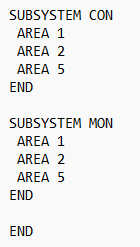
\includegraphics[scale=0.65]{sub.png}
   \caption{The subsystem file corresponding to Year 4 Topology 5} 
   \label{fig:sub}
\end{figure}

\begin{figure}[H]
   \centering 
   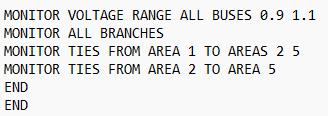
\includegraphics[scale=0.65]{mon.png}
   \caption{The monitored file corresponding to Year 4 Topology 5} 
   \label{fig:mon}
\end{figure}

\begin{figure}[H]
   \centering 
   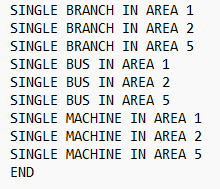
\includegraphics[scale=0.65]{con.png}
   \caption{The contingency file corresponding to Year 4 Topology 5} 
   \label{fig:con}
\end{figure}


For each of the 81 studied scenarios, the API DFAX\_2 is used to construct 81 different distribution factor data files corresponding to each .sav file, and the above defined .sub, .mon, .con configuration files.
For each of the 81 scenarios, by running the AC contingency calculation function ACCC\_WITH\_DSP\_3, the contingency solution output .acc files are obtained.

For each of the 81 scenarios, using the contingency solution output files, the results are exported as excel files for further analysis. The results exported are ACCC Analysis Summary, Monitored Branch Flows (MVA), Monitored Bus Voltages. 
 \newpage
Python code to conduct AC contingency calculation is:

\begin{python}
import psspy
list_gens = [0,50,100]
list_lsc = ['LLS','RLS','HLS']
list_gen_hydro = [400,500,600] #dry, average, wet hydological scenarios
list_gen_wind = [0,40,75] # for 3 wind gust scenarios
for gen in list_gens:
    for gen_hy in list_gen_hydro:
        for lsc in list_lsc:
            for gen_wi in list_gen_wind:
                file_in = 'sav\savnw_sol_' + str(gen) +'_hy_' +str(gen_hy) +'_wi_' + str(gen_wi) +'_' + str(lsc)+'.sav'
                file_dist = 'savnw_sol_' + str(gen) +'_hy_' +str(gen_hy) +'_wi_' + str(gen_wi) +'_' + str(lsc)+'.dfx'
                file_out = 'savnw_sol_' + str(gen) +'_hy_' +str(gen_hy) +'_wi_' + str(gen_wi) +'_' + str(lsc)+'.acc'
                file_sav = r"{}".format(file_in)
                file_dfx = r"{}".format(file_dist)
                file_acc = r"{}".format(file_out)
                psspy.case(file_in)
                psspy.fdns([0,1,0,0,0,0,0,0])
                psspy.dfax_2([1,1,0],r"""savnw.sub""",r"""savnw.mon""",r"""savnw.con""",file_dfx)
                psspy.accc_with_dsp_3(0.1,[0,1,0,0,0,0,0,0,0,0,0],"",file_dfx,file_acc,"","","")
\end{python}



Python code to export AC contingency solution output file as excel is: 

\begin{python}
import pssexcel
list_gens = [0,50,100]
list_lsc = ['LLS','RLS','HLS']
list_gen_hydro = [400,500,600] #dry, average, wet hydological scenarios
list_gen_wind = [0,40,75] # for 3 wind gust scenarios
for gen in list_gens:
    for gen_hy in list_gen_hydro:
        for lsc in list_lsc:
            for gen_wi in list_gen_wind:
                file_in = 'acc\savnw_sol_' + str(gen) +'_hy_' +str(gen_hy) +'_wi_' + str(gen_wi) +'_' + str(lsc)+'.acc'
                file_out = 'savnw_sol_' + str(gen) +'_hy_' +str(gen_hy) +'_wi_' + str(gen_wi) +'_' + str(lsc)+'.xlsx'
                file_acc = r"{}".format(file_in)
                file_xlsx = r"{}".format(file_out)
                pssexcel.accc(file_acc, ['s','v','b'], colabel='',stype='contingency', busmsm=0.5, sysmsm=5.0,
                        rating='a', namesplit=False,xlsfile=file_out, sheet='', overwritesheet=True, show=False, ratecon='b',
                        baseflowvio=True,basevoltvio=True, flowlimit=100.0, flowchange=0.0, voltchange=0.0,swdrating='a',
                        swdratecon='b',baseswdflowvio=False,basenodevoltvio=False,overloadreport=False)
\end{python}

Contingency analysis was carried out in PSSE for each of the studied scenario for Year 4, Topology 5. It was seen that the power flow solution did not converge for some of the tested contingencies for the studied scenario. 
For each of the scenario, the contingencies for which power flow solution did not converge are given in Tables \ref{nonconv}, \ref{nonconv1}, and \ref{nonconv2} Appendix \ref{chapter:app} of the document. 

For the converged contingencies for each of the studied scenario, the results of the contingency analysis were analysed to check for branch overload ($ > 100\%$) and out of range bus voltage violations (lower emergency limit $ < 0.9 PU $ and upper emergency limit $ > 1.1 PU$). It was seen that for some of the contingencies there were no branch overload or bus voltage violations reported. Rest of the contingencies violating branch overload and bus voltage emergency ranges are reported in the subsequent chapters. Chapter ~\ref{overload} of this document gives the observed branch flow violations for each of the studied scenario. Chapter ~\ref{upper} gives the upper voltage violations reported for each of the studied scenarios. Chapter ~\ref{lower} gives the lower voltage violations reported for each of the studied scenarios. To conclude, Chapter ~\ref{conclusion} summarises the result of the contingency analysis carried out on Year 4, Topology 5 of the hypothetical SAVNW system. 



\chapter{Branch Overload Violation}
\label{overload}
\section{Introduction}
In this chapter, for each of the studied scenario, the branches that are loaded more than 100\% of their rating is tabulated. Branches that are loaded more than 130\% of the rating are said to be severely/ critically loaded and are noted down for reporting as operating these branches for prolonged duration is not recommended for a safe and reliable power system.
\section{Solar = 0 MW, Hydro = 400 MW, Wind = 0 MW, LLS}
For the studied scenario Solar = 0 MW, Hydro = 400 MW, Wind = 0 MW, LLS, the branches that are loaded more than 100\% of their rating is given in Table ~\ref{OLSolar0MWHydro400MWWind0MWLLS}. A loading of greater than 130\% of the branch rating was reported for the branch 154-203(1) for bus fault contingency BUS 205.
\begin{table}[H]
\caption{Contingencies causing branch flow greater than 100\% for scenario Solar = 0 MW, Hydro = 400 MW, Wind = 0 MW, LLS}
\label{OLSolar0MWHydro400MWWind0MWLLS}
\centering
\scalebox{0.75}{\begin{tabular}{llrrrr}
\toprule
Branch & Contingency & MVA Flow & AMP Flow & Rate & Loading \\
\midrule
3001-3003(1) & SING OPN LIN   1 101-151(1) & 356.86 & 348.61 & 300.00 & 116.20 \\
3001-3003(2) & SING OPN LIN   1 101-151(1) & 356.86 & 348.61 & 300.00 & 116.20 \\
101-151(1) & SING OPN LIN   2 102-151(1) & 1456.61 & 1456.61 & 1350.00 & 107.90 \\
154-203(1) & SING OPN LIN   6 152-153(1) & 288.43 & 306.12 & 250.00 & 122.45 \\
154-205(1) & SING OPN LIN   6 152-153(1) & 718.74 & 762.82 & 660.00 & 115.58 \\
154-203(1) & SING OPN LIN   11 201-204(1) & 245.80 & 293.05 & 250.00 & 117.22 \\
203-205(1) & SING OPN LIN   11 201-204(1) & -225.99 & 268.11 & 250.00 & 107.24 \\
203-205(2) & SING OPN LIN   11 201-204(1) & -225.99 & 268.11 & 250.00 & 107.24 \\
154-203(1) & BUS 153 & 270.85 & 281.66 & 250.00 & 112.66 \\
154-205(1) & BUS 153 & 644.70 & 670.42 & 660.00 & 101.58 \\
154-203(1) & BUS 204 & 245.81 & 293.07 & 250.00 & 117.23 \\
203-205(1) & BUS 204 & -226.01 & 268.14 & 250.00 & 107.26 \\
203-205(2) & BUS 204 & -226.01 & 268.14 & 250.00 & 107.26 \\
154-203(1) & BUS 205 & 369.02 & 452.10 & 250.00 & 180.84 \\
3001-3003(1) & UNIT 101(1) & 356.91 & 348.66 & 300.00 & 116.22 \\
3001-3003(2) & UNIT 101(1) & 356.91 & 348.66 & 300.00 & 116.22 \\
101-151(1) & UNIT 102(1) & 1456.61 & 1456.61 & 1350.00 & 107.90 \\
\bottomrule
\end{tabular}}
\end{table}

\section{Solar = 0 MW, Hydro = 400 MW, Wind = 40 MW, LLS}
For the studied scenario Solar = 0 MW, Hydro = 400 MW, Wind = 40 MW, LLS, the branches that are loaded more than 100\% of their rating is given in Table ~\ref{OLSolar0MWHydro400MWWind40MWLLS}. A loading of greater than 130\% of the branch rating was reported for the branch 154-203(1) for bus fault contingency BUS 205.
\begin{table}[H]
\caption{Contingencies causing branch flow greater than 100\% for scenario Solar = 0 MW, Hydro = 400 MW, Wind = 40 MW, LLS}
\label{OLSolar0MWHydro400MWWind40MWLLS}
\centering
\scalebox{0.75}{\begin{tabular}{llrrrr}
\toprule
Branch & Contingency & MVA Flow & AMP Flow & Rate & Loading \\
\midrule
3001-3003(1) & SING OPN LIN   1 101-151(1) & 342.27 & 333.95 & 300.00 & 111.32 \\
3001-3003(2) & SING OPN LIN   1 101-151(1) & 342.27 & 333.95 & 300.00 & 111.32 \\
101-151(1) & SING OPN LIN   2 102-151(1) & 1456.68 & 1456.68 & 1350.00 & 107.90 \\
154-203(1) & SING OPN LIN   6 152-153(1) & 286.39 & 303.45 & 250.00 & 121.38 \\
154-205(1) & SING OPN LIN   6 152-153(1) & 713.00 & 755.48 & 660.00 & 114.47 \\
154-203(1) & SING OPN LIN   11 201-204(1) & 246.16 & 293.45 & 250.00 & 117.38 \\
203-205(1) & SING OPN LIN   11 201-204(1) & -226.27 & 268.42 & 250.00 & 107.37 \\
203-205(2) & SING OPN LIN   11 201-204(1) & -226.27 & 268.42 & 250.00 & 107.37 \\
154-203(1) & BUS 153 & 270.43 & 281.09 & 250.00 & 112.43 \\
154-205(1) & BUS 153 & 643.42 & 668.78 & 660.00 & 101.33 \\
154-203(1) & BUS 204 & 246.17 & 293.47 & 250.00 & 117.39 \\
203-205(1) & BUS 204 & -226.29 & 268.45 & 250.00 & 107.38 \\
203-205(2) & BUS 204 & -226.29 & 268.45 & 250.00 & 107.38 \\
154-203(1) & BUS 205 & 370.01 & 455.49 & 250.00 & 182.20 \\
3001-3003(1) & UNIT 101(1) & 342.31 & 334.00 & 300.00 & 111.33 \\
3001-3003(2) & UNIT 101(1) & 342.31 & 334.00 & 300.00 & 111.33 \\
101-151(1) & UNIT 102(1) & 1456.68 & 1456.68 & 1350.00 & 107.90 \\
\bottomrule
\end{tabular}}
\end{table}

\section{Solar = 0 MW, Hydro = 400 MW, Wind = 75 MW, LLS}
For the studied scenario Solar = 0 MW, Hydro = 400 MW, Wind = 75 MW, LLS, the branches that are loaded more than 100\% of their rating is given in Table ~\ref{OLSolar0MWHydro400MWWind75MWLLS}. A loading of greater than 130\% of the branch rating was reported for the branch 154-203(1) for bus fault contingency BUS 205.
\begin{table}[H]
\caption{Contingencies causing branch flow greater than 100\% for scenario Solar = 0 MW, Hydro = 400 MW, Wind = 75 MW, LLS}
\label{OLSolar0MWHydro400MWWind75MWLLS}
\centering
\scalebox{0.75}{\begin{tabular}{llrrrr}
\toprule
Branch & Contingency & MVA Flow & AMP Flow & Rate & Loading \\
\midrule
3001-3003(1) & SING OPN LIN   1 101-151(1) & 329.83 & 321.53 & 300.00 & 107.18 \\
3001-3003(2) & SING OPN LIN   1 101-151(1) & 329.83 & 321.53 & 300.00 & 107.18 \\
101-151(1) & SING OPN LIN   2 102-151(1) & 1456.79 & 1456.79 & 1350.00 & 107.91 \\
154-203(1) & SING OPN LIN   6 152-153(1) & 284.78 & 301.69 & 250.00 & 120.68 \\
154-205(1) & SING OPN LIN   6 152-153(1) & 709.21 & 751.31 & 660.00 & 113.84 \\
154-203(1) & SING OPN LIN   11 201-204(1) & 246.62 & 294.99 & 250.00 & 117.99 \\
203-205(1) & SING OPN LIN   11 201-204(1) & -226.63 & 269.75 & 250.00 & 107.90 \\
203-205(2) & SING OPN LIN   11 201-204(1) & -226.63 & 269.75 & 250.00 & 107.90 \\
154-203(1) & BUS 153 & 270.15 & 280.87 & 250.00 & 112.35 \\
154-205(1) & BUS 153 & 642.98 & 668.49 & 660.00 & 101.29 \\
154-203(1) & BUS 204 & 246.62 & 295.01 & 250.00 & 118.00 \\
203-205(1) & BUS 204 & -226.63 & 269.77 & 250.00 & 107.91 \\
203-205(2) & BUS 204 & -226.63 & 269.77 & 250.00 & 107.91 \\
154-203(1) & BUS 205 & 371.08 & 460.07 & 250.00 & 184.03 \\
3001-3003(1) & UNIT 101(1) & 329.88 & 321.58 & 300.00 & 107.19 \\
3001-3003(2) & UNIT 101(1) & 329.88 & 321.58 & 300.00 & 107.19 \\
101-151(1) & UNIT 102(1) & 1456.79 & 1456.79 & 1350.00 & 107.91 \\
\bottomrule
\end{tabular}}
\end{table}

\section{Solar = 0 MW, Hydro = 400 MW, Wind = 0 MW, RLS}
For the studied scenario Solar = 0 MW, Hydro = 400 MW, Wind = 0 MW, RLS, the branches that are loaded more than 100\% of their rating is given in Table ~\ref{OLSolar0MWHydro400MWWind0MWRLS}. A loading of greater than 130\% of the branch rating was reported for the branch 154-203(1) for single line open contingency SING OPN LIN   6 152-153(1).
\begin{table}[H]
\caption{Contingencies causing branch flow greater than 100\% for scenario Solar = 0 MW, Hydro = 400 MW, Wind = 0 MW, RLS}
\label{OLSolar0MWHydro400MWWind0MWRLS}
\centering
\scalebox{0.75}{\begin{tabular}{llrrrr}
\toprule
Branch & Contingency & MVA Flow & AMP Flow & Rate & Loading \\
\midrule
3001-3003(1) & SING OPN LIN   1 101-151(1) & 391.59 & 384.29 & 300.00 & 128.10 \\
3001-3003(2) & SING OPN LIN   1 101-151(1) & 391.59 & 384.29 & 300.00 & 128.10 \\
3003-3005(1) & SING OPN LIN   1 101-151(1) & -379.03 & 384.56 & 350.00 & 109.87 \\
3003-3005(2) & SING OPN LIN   1 101-151(1) & -379.03 & 384.56 & 350.00 & 109.87 \\
101-151(1) & SING OPN LIN   2 102-151(1) & 1525.81 & 1525.81 & 1350.00 & 113.02 \\
154-203(1) & SING OPN LIN   6 152-153(1) & 299.59 & 332.48 & 250.00 & 132.99 \\
154-205(1) & SING OPN LIN   6 152-153(1) & 768.37 & 852.73 & 660.00 & 129.20 \\
154-203(1) & BUS 153 & 282.16 & 305.08 & 250.00 & 122.03 \\
154-205(1) & BUS 153 & 690.37 & 746.46 & 660.00 & 113.10 \\
153-154(1) & BUS 203 & -324.50 & 351.86 & 350.00 & 100.53 \\
3001-3003(1) & UNIT 101(1) & 391.66 & 384.37 & 300.00 & 128.12 \\
3001-3003(2) & UNIT 101(1) & 391.66 & 384.37 & 300.00 & 128.12 \\
3003-3005(1) & UNIT 101(1) & -379.10 & 384.64 & 350.00 & 109.90 \\
3003-3005(2) & UNIT 101(1) & -379.10 & 384.64 & 350.00 & 109.90 \\
101-151(1) & UNIT 102(1) & 1525.81 & 1525.81 & 1350.00 & 113.02 \\
\bottomrule
\end{tabular}}
\end{table}

\section{Solar = 0 MW, Hydro = 400 MW, Wind = 40 MW, RLS}
For the studied scenario Solar = 0 MW, Hydro = 400 MW, Wind = 40 MW, RLS, the branches that are loaded more than 100\% of their rating is given in Table ~\ref{OLSolar0MWHydro400MWWind40MWRLS}. A loading of greater than 130\% of the branch rating was reported for the branch 154-203(1) for single line open contingency SING OPN LIN   6 152-153(1).
\begin{table}[H]
\caption{Contingencies causing branch flow greater than 100\% for scenario Solar = 0 MW, Hydro = 400 MW, Wind = 40 MW, RLS}
\label{OLSolar0MWHydro400MWWind40MWRLS}
\centering
\scalebox{0.75}{\begin{tabular}{llrrrr}
\toprule
Branch & Contingency & MVA Flow & AMP Flow & Rate & Loading \\
\midrule
3001-3003(1) & SING OPN LIN   1 101-151(1) & 376.83 & 369.16 & 300.00 & 123.05 \\
3001-3003(2) & SING OPN LIN   1 101-151(1) & 376.83 & 369.16 & 300.00 & 123.05 \\
3003-3005(1) & SING OPN LIN   1 101-151(1) & -365.33 & 369.43 & 350.00 & 105.55 \\
3003-3005(2) & SING OPN LIN   1 101-151(1) & -365.33 & 369.43 & 350.00 & 105.55 \\
101-151(1) & SING OPN LIN   2 102-151(1) & 1525.80 & 1525.80 & 1350.00 & 113.02 \\
154-203(1) & SING OPN LIN   6 152-153(1) & 297.57 & 329.51 & 250.00 & 131.81 \\
154-205(1) & SING OPN LIN   6 152-153(1) & 762.50 & 844.36 & 660.00 & 127.93 \\
154-203(1) & BUS 153 & 281.74 & 304.45 & 250.00 & 121.78 \\
154-205(1) & BUS 153 & 689.08 & 744.62 & 660.00 & 112.82 \\
153-154(1) & BUS 203 & -326.44 & 353.89 & 350.00 & 101.11 \\
3001-3003(1) & UNIT 101(1) & 376.90 & 369.24 & 300.00 & 123.08 \\
3001-3003(2) & UNIT 101(1) & 376.90 & 369.24 & 300.00 & 123.08 \\
3003-3005(1) & UNIT 101(1) & -365.40 & 369.50 & 350.00 & 105.57 \\
3003-3005(2) & UNIT 101(1) & -365.40 & 369.50 & 350.00 & 105.57 \\
101-151(1) & UNIT 102(1) & 1525.80 & 1525.80 & 1350.00 & 113.02 \\
\bottomrule
\end{tabular}}
\end{table}

\section{Solar = 0 MW, Hydro = 400 MW, Wind = 75 MW, RLS}
For the studied scenario Solar = 0 MW, Hydro = 400 MW, Wind = 75 MW, RLS, the branches that are loaded more than 100\% of their rating is given in Table ~\ref{OLSolar0MWHydro400MWWind75MWRLS}. A loading of greater than 130\% of the branch rating was reported for the branch 154-203(1) for single line open contingency SING OPN LIN   6 152-153(1).
\begin{table}[H]
\caption{Contingencies causing branch flow greater than 100\% for scenario Solar = 0 MW, Hydro = 400 MW, Wind = 75 MW, RLS}
\label{OLSolar0MWHydro400MWWind75MWRLS}
\centering
\scalebox{0.75}{\begin{tabular}{llrrrr}
\toprule
Branch & Contingency & MVA Flow & AMP Flow & Rate & Loading \\
\midrule
3001-3003(1) & SING OPN LIN   1 101-151(1) & 364.11 & 356.25 & 300.00 & 118.75 \\
3001-3003(2) & SING OPN LIN   1 101-151(1) & 364.11 & 356.25 & 300.00 & 118.75 \\
3003-3005(1) & SING OPN LIN   1 101-151(1) & -353.34 & 356.54 & 350.00 & 101.87 \\
3003-3005(2) & SING OPN LIN   1 101-151(1) & -353.34 & 356.54 & 350.00 & 101.87 \\
101-151(1) & SING OPN LIN   2 102-151(1) & 1525.93 & 1525.93 & 1350.00 & 113.03 \\
154-203(1) & SING OPN LIN   6 152-153(1) & 296.02 & 327.72 & 250.00 & 131.09 \\
154-205(1) & SING OPN LIN   6 152-153(1) & 758.68 & 839.92 & 660.00 & 127.26 \\
154-203(1) & BUS 153 & 281.50 & 304.27 & 250.00 & 121.71 \\
154-205(1) & BUS 153 & 688.64 & 744.35 & 660.00 & 112.78 \\
153-154(1) & BUS 203 & -327.99 & 355.82 & 350.00 & 101.66 \\
3001-3003(1) & UNIT 101(1) & 364.18 & 356.32 & 300.00 & 118.77 \\
3001-3003(2) & UNIT 101(1) & 364.18 & 356.32 & 300.00 & 118.77 \\
3003-3005(1) & UNIT 101(1) & -353.41 & 356.61 & 350.00 & 101.89 \\
3003-3005(2) & UNIT 101(1) & -353.41 & 356.61 & 350.00 & 101.89 \\
101-151(1) & UNIT 102(1) & 1525.93 & 1525.93 & 1350.00 & 113.03 \\
\bottomrule
\end{tabular}}
\end{table}

\section{Solar = 0 MW, Hydro = 400 MW, Wind = 0 MW, HLS}
For the studied scenario Solar = 0 MW, Hydro = 400 MW, Wind = 0 MW, HLS, the branches that are loaded more than 100\% of their rating is given in Table ~\ref{OLSolar0MWHydro400MWWind0MWHLS}. A loading of greater than 130\% of the branch rating were reported for the branches: 154-203(1) for bus fault contingency BUS 153; 154-203(1), 154-205(1) for single line open contingency SING OPN LIN   6 152-153(1); 3001-3003(1), 3001-3003(2) for single line open contingency SING OPN LIN   1 101-151(1); 3001-3003(1), 3001-3003(2) for unit fault contingency UNIT 101(1).
\begin{table}[H]
\caption{Contingencies causing branch flow greater than 100\% for scenario Solar = 0 MW, Hydro = 400 MW, Wind = 0 MW, HLS}
\label{OLSolar0MWHydro400MWWind0MWHLS}
\centering
\scalebox{0.75}{\begin{tabular}{llrrrr}
\toprule
Branch & Contingency & MVA Flow & AMP Flow & Rate & Loading \\
\midrule
3001-3003(1) & SING OPN LIN   1 101-151(1) & 423.37 & 418.96 & 300.00 & 139.65 \\
3001-3003(2) & SING OPN LIN   1 101-151(1) & 423.37 & 418.96 & 300.00 & 139.65 \\
3003-3005(1) & SING OPN LIN   1 101-151(1) & -404.55 & 419.55 & 350.00 & 119.87 \\
3003-3005(2) & SING OPN LIN   1 101-151(1) & -404.55 & 419.55 & 350.00 & 119.87 \\
101-151(1) & SING OPN LIN   2 102-151(1) & 1586.00 & 1586.00 & 1350.00 & 117.48 \\
154-203(1) & SING OPN LIN   6 152-153(1) & 309.33 & 359.66 & 250.00 & 143.86 \\
154-205(1) & SING OPN LIN   6 152-153(1) & 807.05 & 938.37 & 660.00 & 142.18 \\
203-205(1) & SING OPN LIN   6 152-153(1) & -219.15 & 250.25 & 250.00 & 100.10 \\
203-205(2) & SING OPN LIN   6 152-153(1) & -219.15 & 250.25 & 250.00 & 100.10 \\
154-205(1) & SING OPN LIN   10 201-202(1) & 555.27 & 684.03 & 660.00 & 103.64 \\
205-206(1) & SING OPN LIN   12 201-211(1) & -1281.54 & 1281.54 & 1250.00 & 102.52 \\
205-206(1) & SING OPN LIN   13 201-212(1) & -1281.54 & 1281.54 & 1250.00 & 102.52 \\
154-203(1) & BUS 153 & 292.09 & 328.20 & 250.00 & 131.28 \\
154-205(1) & BUS 153 & 726.38 & 816.18 & 660.00 & 123.66 \\
153-154(1) & BUS 203 & -334.86 & 376.78 & 350.00 & 107.65 \\
154-203(1) & BUS 3005 & 227.22 & 267.87 & 250.00 & 107.15 \\
154-205(1) & BUS 3005 & 633.84 & 747.23 & 660.00 & 113.22 \\
154-3008(1) & BUS 3005 & -359.80 & 448.00 & 440.00 & 101.82 \\
3001-3003(1) & UNIT 101(1) & 423.52 & 419.11 & 300.00 & 139.70 \\
3001-3003(2) & UNIT 101(1) & 423.52 & 419.11 & 300.00 & 139.70 \\
3003-3005(1) & UNIT 101(1) & -404.68 & 419.70 & 350.00 & 119.92 \\
3003-3005(2) & UNIT 101(1) & -404.68 & 419.70 & 350.00 & 119.92 \\
101-151(1) & UNIT 102(1) & 1585.99 & 1585.99 & 1350.00 & 117.48 \\
205-206(1) & UNIT 211(1) & -1281.65 & 1281.65 & 1250.00 & 102.53 \\
205-206(1) & UNIT 212(1) & -1281.65 & 1281.65 & 1250.00 & 102.53 \\
\bottomrule
\end{tabular}}
\end{table}

\section{Solar = 0 MW, Hydro = 400 MW, Wind = 40 MW, HLS}
For the studied scenario Solar = 0 MW, Hydro = 400 MW, Wind = 40 MW, HLS, the branches that are loaded more than 100\% of their rating is given in Table ~\ref{OLSolar0MWHydro400MWWind40MWHLS}. A loading of greater than 130\% of the branch rating were reported for the branches: 154-203(1) for bus fault contingency BUS 153; 154-203(1), 154-205(1) for single line open contingency SING OPN LIN   6 152-153(1); 3001-3003(1), 3001-3003(2) for single line open contingency SING OPN LIN   1 101-151(1); 3001-3003(1), 3001-3003(2) for unit fault contingency UNIT 101(1).
\begin{table}[H]
\caption{Contingencies causing branch flow greater than 100\% for scenario Solar = 0 MW, Hydro = 400 MW, Wind = 40 MW, HLS}
\label{OLSolar0MWHydro400MWWind40MWHLS}
\centering
\scalebox{0.75}{\begin{tabular}{llrrrr}
\toprule
Branch & Contingency & MVA Flow & AMP Flow & Rate & Loading \\
\midrule
3001-3003(1) & SING OPN LIN   1 101-151(1) & 408.03 & 402.92 & 300.00 & 134.31 \\
3001-3003(2) & SING OPN LIN   1 101-151(1) & 408.03 & 402.92 & 300.00 & 134.31 \\
3003-3005(1) & SING OPN LIN   1 101-151(1) & -390.71 & 403.52 & 350.00 & 115.29 \\
3003-3005(2) & SING OPN LIN   1 101-151(1) & -390.71 & 403.52 & 350.00 & 115.29 \\
101-151(1) & SING OPN LIN   2 102-151(1) & 1585.95 & 1585.95 & 1350.00 & 117.48 \\
154-203(1) & SING OPN LIN   6 152-153(1) & 307.33 & 356.27 & 250.00 & 142.51 \\
154-205(1) & SING OPN LIN   6 152-153(1) & 801.11 & 928.69 & 660.00 & 140.71 \\
154-205(1) & SING OPN LIN   10 201-202(1) & 555.85 & 684.26 & 660.00 & 103.68 \\
205-206(1) & SING OPN LIN   12 201-211(1) & -1282.59 & 1282.59 & 1250.00 & 102.61 \\
205-206(1) & SING OPN LIN   13 201-212(1) & -1282.59 & 1282.59 & 1250.00 & 102.61 \\
154-203(1) & BUS 153 & 291.68 & 327.49 & 250.00 & 130.99 \\
154-205(1) & BUS 153 & 725.07 & 814.08 & 660.00 & 123.35 \\
153-154(1) & BUS 203 & -336.70 & 378.76 & 350.00 & 108.22 \\
154-203(1) & BUS 3005 & 226.14 & 265.64 & 250.00 & 106.26 \\
154-205(1) & BUS 3005 & 630.42 & 740.53 & 660.00 & 112.20 \\
154-3008(1) & BUS 3005 & -359.66 & 445.93 & 440.00 & 101.35 \\
3001-3003(1) & UNIT 101(1) & 408.17 & 403.07 & 300.00 & 134.36 \\
3001-3003(2) & UNIT 101(1) & 408.17 & 403.07 & 300.00 & 134.36 \\
3003-3005(1) & UNIT 101(1) & -390.84 & 403.67 & 350.00 & 115.33 \\
3003-3005(2) & UNIT 101(1) & -390.84 & 403.67 & 350.00 & 115.33 \\
101-151(1) & UNIT 102(1) & 1585.95 & 1585.95 & 1350.00 & 117.48 \\
205-206(1) & UNIT 211(1) & -1281.51 & 1281.51 & 1250.00 & 102.52 \\
205-206(1) & UNIT 212(1) & -1281.51 & 1281.51 & 1250.00 & 102.52 \\
\bottomrule
\end{tabular}}
\end{table}

\section{Solar = 0 MW, Hydro = 400 MW, Wind = 75 MW, HLS}
For the studied scenario Solar = 0 MW, Hydro = 400 MW, Wind = 75 MW, HLS, the branches that are loaded more than 100\% of their rating is given in Table ~\ref{OLSolar0MWHydro400MWWind75MWHLS}. A loading of greater than 130\% of the branch rating were reported for the branches: 154-203(1) for bus fault contingency BUS 153; 154-203(1), 154-205(1) for single line open contingency SING OPN LIN   6 152-153(1).
\begin{table}[H]
\caption{Contingencies causing branch flow greater than 100\% for scenario Solar = 0 MW, Hydro = 400 MW, Wind = 75 MW, HLS}
\label{OLSolar0MWHydro400MWWind75MWHLS}
\centering
\scalebox{0.75}{\begin{tabular}{llrrrr}
\toprule
Branch & Contingency & MVA Flow & AMP Flow & Rate & Loading \\
\midrule
3001-3003(1) & SING OPN LIN   1 101-151(1) & 395.17 & 389.64 & 300.00 & 129.88 \\
3001-3003(2) & SING OPN LIN   1 101-151(1) & 395.17 & 389.64 & 300.00 & 129.88 \\
3003-3005(1) & SING OPN LIN   1 101-151(1) & -378.87 & 390.25 & 350.00 & 111.50 \\
3003-3005(2) & SING OPN LIN   1 101-151(1) & -378.87 & 390.25 & 350.00 & 111.50 \\
101-151(1) & SING OPN LIN   2 102-151(1) & 1586.12 & 1586.12 & 1350.00 & 117.49 \\
154-203(1) & SING OPN LIN   6 152-153(1) & 305.85 & 354.44 & 250.00 & 141.78 \\
154-205(1) & SING OPN LIN   6 152-153(1) & 797.28 & 923.95 & 660.00 & 139.99 \\
205-206(1) & SING OPN LIN   12 201-211(1) & -1282.54 & 1282.54 & 1250.00 & 102.60 \\
205-206(1) & SING OPN LIN   13 201-212(1) & -1282.54 & 1282.54 & 1250.00 & 102.60 \\
154-203(1) & BUS 153 & 291.46 & 327.35 & 250.00 & 130.94 \\
154-205(1) & BUS 153 & 724.63 & 813.86 & 660.00 & 123.31 \\
153-154(1) & BUS 203 & -338.17 & 380.74 & 350.00 & 108.78 \\
154-203(1) & BUS 3005 & 225.54 & 264.81 & 250.00 & 105.92 \\
154-205(1) & BUS 3005 & 628.76 & 738.21 & 660.00 & 111.85 \\
154-3008(1) & BUS 3005 & -359.65 & 445.66 & 440.00 & 101.29 \\
3001-3003(1) & UNIT 101(1) & 395.31 & 389.78 & 300.00 & 129.93 \\
3001-3003(2) & UNIT 101(1) & 395.31 & 389.78 & 300.00 & 129.93 \\
3003-3005(1) & UNIT 101(1) & -378.99 & 390.40 & 350.00 & 111.54 \\
3003-3005(2) & UNIT 101(1) & -378.99 & 390.40 & 350.00 & 111.54 \\
101-151(1) & UNIT 102(1) & 1586.12 & 1586.12 & 1350.00 & 117.49 \\
205-206(1) & UNIT 211(1) & -1281.41 & 1281.41 & 1250.00 & 102.51 \\
205-206(1) & UNIT 212(1) & -1281.41 & 1281.41 & 1250.00 & 102.51 \\
\bottomrule
\end{tabular}}
\end{table}

\section{Solar = 0 MW, Hydro = 500 MW, Wind = 0 MW, LLS}
For the studied scenario Solar = 0 MW, Hydro = 500 MW, Wind = 0 MW, LLS, the branches that are loaded more than 100\% of their rating is given in Table ~\ref{OLSolar0MWHydro500MWWind0MWLLS}. A loading of greater than 130\% of the branch rating was reported for the branch 154-203(1) for single line open contingency SING OPN LIN   6 152-153(1).
\begin{table}[H]
\caption{Contingencies causing branch flow greater than 100\% for scenario Solar = 0 MW, Hydro = 500 MW, Wind = 0 MW, LLS}
\label{OLSolar0MWHydro500MWWind0MWLLS}
\centering
\scalebox{0.75}{\begin{tabular}{llrrrr}
\toprule
Branch & Contingency & MVA Flow & AMP Flow & Rate & Loading \\
\midrule
3001-3003(1) & SING OPN LIN   1 101-151(1) & 358.42 & 350.27 & 300.00 & 116.76 \\
3001-3003(2) & SING OPN LIN   1 101-151(1) & 358.42 & 350.27 & 300.00 & 116.76 \\
3003-3005(1) & SING OPN LIN   1 101-151(1) & -348.43 & 350.50 & 350.00 & 100.14 \\
3003-3005(2) & SING OPN LIN   1 101-151(1) & -348.43 & 350.50 & 350.00 & 100.14 \\
101-151(1) & SING OPN LIN   2 102-151(1) & 1459.79 & 1459.79 & 1350.00 & 108.13 \\
154-203(1) & SING OPN LIN   6 152-153(1) & 310.72 & 334.90 & 250.00 & 133.96 \\
154-205(1) & SING OPN LIN   6 152-153(1) & 674.23 & 726.70 & 660.00 & 110.11 \\
154-203(1) & BUS 153 & 295.04 & 311.21 & 250.00 & 124.48 \\
153-154(1) & BUS 203 & -339.81 & 363.09 & 350.00 & 103.74 \\
3001-3003(1) & UNIT 101(1) & 358.47 & 350.33 & 300.00 & 116.78 \\
3001-3003(2) & UNIT 101(1) & 358.47 & 350.33 & 300.00 & 116.78 \\
3003-3005(1) & UNIT 101(1) & -348.48 & 350.56 & 350.00 & 100.16 \\
3003-3005(2) & UNIT 101(1) & -348.48 & 350.56 & 350.00 & 100.16 \\
101-151(1) & UNIT 102(1) & 1459.79 & 1459.79 & 1350.00 & 108.13 \\
\bottomrule
\end{tabular}}
\end{table}

\section{Solar = 0 MW, Hydro = 500 MW, Wind = 40 MW, LLS}
For the studied scenario Solar = 0 MW, Hydro = 500 MW, Wind = 40 MW, LLS, the branches that are loaded more than 100\% of their rating is given in Table ~\ref{OLSolar0MWHydro500MWWind40MWLLS}. A loading of greater than 130\% of the branch rating was reported for the branch 154-203(1) for single line open contingency SING OPN LIN   6 152-153(1).
\begin{table}[H]
\caption{Contingencies causing branch flow greater than 100\% for scenario Solar = 0 MW, Hydro = 500 MW, Wind = 40 MW, LLS}
\label{OLSolar0MWHydro500MWWind40MWLLS}
\centering
\scalebox{0.75}{\begin{tabular}{llrrrr}
\toprule
Branch & Contingency & MVA Flow & AMP Flow & Rate & Loading \\
\midrule
3001-3003(1) & SING OPN LIN   1 101-151(1) & 343.82 & 335.60 & 300.00 & 111.87 \\
3001-3003(2) & SING OPN LIN   1 101-151(1) & 343.82 & 335.60 & 300.00 & 111.87 \\
101-151(1) & SING OPN LIN   2 102-151(1) & 1459.86 & 1459.86 & 1350.00 & 108.14 \\
154-203(1) & SING OPN LIN   6 152-153(1) & 308.71 & 332.12 & 250.00 & 132.85 \\
154-205(1) & SING OPN LIN   6 152-153(1) & 668.48 & 719.17 & 660.00 & 108.97 \\
154-203(1) & BUS 153 & 294.62 & 310.61 & 250.00 & 124.25 \\
153-154(1) & BUS 203 & -341.82 & 365.18 & 350.00 & 104.34 \\
3001-3003(1) & UNIT 101(1) & 343.87 & 335.65 & 300.00 & 111.88 \\
3001-3003(2) & UNIT 101(1) & 343.87 & 335.65 & 300.00 & 111.88 \\
101-151(1) & UNIT 102(1) & 1459.86 & 1459.86 & 1350.00 & 108.14 \\
\bottomrule
\end{tabular}}
\end{table}

\section{Solar = 0 MW, Hydro = 500 MW, Wind = 75 MW, LLS}
For the studied scenario Solar = 0 MW, Hydro = 500 MW, Wind = 75 MW, LLS, the branches that are loaded more than 100\% of their rating is given in Table ~\ref{OLSolar0MWHydro500MWWind75MWLLS}. A loading of greater than 130\% of the branch rating was reported for the branch 154-203(1) for single line open contingency SING OPN LIN   6 152-153(1).
\begin{table}[H]
\caption{Contingencies causing branch flow greater than 100\% for scenario Solar = 0 MW, Hydro = 500 MW, Wind = 75 MW, LLS}
\label{OLSolar0MWHydro500MWWind75MWLLS}
\centering
\scalebox{0.75}{\begin{tabular}{llrrrr}
\toprule
Branch & Contingency & MVA Flow & AMP Flow & Rate & Loading \\
\midrule
3001-3003(1) & SING OPN LIN   1 101-151(1) & 331.39 & 323.18 & 300.00 & 107.73 \\
3001-3003(2) & SING OPN LIN   1 101-151(1) & 331.39 & 323.18 & 300.00 & 107.73 \\
101-151(1) & SING OPN LIN   2 102-151(1) & 1459.99 & 1459.99 & 1350.00 & 108.15 \\
154-203(1) & SING OPN LIN   6 152-153(1) & 307.10 & 330.30 & 250.00 & 132.12 \\
154-205(1) & SING OPN LIN   6 152-153(1) & 664.77 & 715.00 & 660.00 & 108.33 \\
154-203(1) & BUS 153 & 294.35 & 310.41 & 250.00 & 124.16 \\
153-154(1) & BUS 203 & -343.45 & 367.19 & 350.00 & 104.91 \\
3001-3003(1) & UNIT 101(1) & 331.44 & 323.23 & 300.00 & 107.74 \\
3001-3003(2) & UNIT 101(1) & 331.44 & 323.23 & 300.00 & 107.74 \\
101-151(1) & UNIT 102(1) & 1459.99 & 1459.99 & 1350.00 & 108.15 \\
\bottomrule
\end{tabular}}
\end{table}

\section{Solar = 0 MW, Hydro = 500 MW, Wind = 0 MW, RLS}
For the studied scenario Solar = 0 MW, Hydro = 500 MW, Wind = 0 MW, RLS, the branches that are loaded more than 100\% of their rating is given in Table ~\ref{OLSolar0MWHydro500MWWind0MWRLS}. A loading of greater than 130\% of the branch rating was reported for the branch 154-203(1) for bus fault contingency BUS 153 and for single line open contingency SING OPN LIN   6 152-153(1).
\begin{table}[H]
\caption{Contingencies causing branch flow greater than 100\% for scenario Solar = 0 MW, Hydro = 500 MW, Wind = 0 MW, RLS}
\label{OLSolar0MWHydro500MWWind0MWRLS}
\centering
\scalebox{0.75}{\begin{tabular}{llrrrr}
\toprule
Branch & Contingency & MVA Flow & AMP Flow & Rate & Loading \\
\midrule
3001-3003(1) & SING OPN LIN   1 101-151(1) & 394.18 & 387.49 & 300.00 & 129.16 \\
3001-3003(2) & SING OPN LIN   1 101-151(1) & 394.18 & 387.49 & 300.00 & 129.16 \\
3003-3005(1) & SING OPN LIN   1 101-151(1) & -380.33 & 387.87 & 350.00 & 110.82 \\
3003-3005(2) & SING OPN LIN   1 101-151(1) & -380.33 & 387.87 & 350.00 & 110.82 \\
101-151(1) & SING OPN LIN   2 102-151(1) & 1530.95 & 1530.95 & 1350.00 & 113.40 \\
154-203(1) & SING OPN LIN   6 152-153(1) & 320.84 & 362.66 & 250.00 & 145.06 \\
154-205(1) & SING OPN LIN   6 152-153(1) & 724.55 & 818.97 & 660.00 & 124.09 \\
203-205(1) & SING OPN LIN   6 152-153(1) & -236.34 & 262.83 & 250.00 & 105.13 \\
203-205(2) & SING OPN LIN   6 152-153(1) & -236.34 & 262.83 & 250.00 & 105.13 \\
154-203(1) & BUS 153 & 305.36 & 335.56 & 250.00 & 134.22 \\
154-205(1) & BUS 153 & 650.36 & 714.68 & 660.00 & 108.28 \\
153-154(1) & BUS 203 & -351.26 & 391.70 & 350.00 & 111.91 \\
154-203(1) & BUS 3005 & 231.05 & 261.73 & 250.00 & 104.69 \\
3001-3003(1) & UNIT 101(1) & 394.27 & 387.58 & 300.00 & 129.19 \\
3001-3003(2) & UNIT 101(1) & 394.27 & 387.58 & 300.00 & 129.19 \\
3003-3005(1) & UNIT 101(1) & -380.41 & 387.96 & 350.00 & 110.85 \\
3003-3005(2) & UNIT 101(1) & -380.41 & 387.96 & 350.00 & 110.85 \\
101-151(1) & UNIT 102(1) & 1530.94 & 1530.94 & 1350.00 & 113.40 \\
\bottomrule
\end{tabular}}
\end{table}

\section{Solar = 0 MW, Hydro = 500 MW, Wind = 40 MW, RLS}
For the studied scenario Solar = 0 MW, Hydro = 500 MW, Wind = 40 MW, RLS, the branches that are loaded more than 100\% of their rating is given in Table ~\ref{OLSolar0MWHydro500MWWind40MWRLS}. A loading of greater than 130\% of the branch rating was reported for the branch 154-203(1) for bus fault contingency BUS 153 and for single line open contingency SING OPN LIN   6 152-153(1).
\begin{table}[H]
\caption{Contingencies causing branch flow greater than 100\% for scenario Solar = 0 MW, Hydro = 500 MW, Wind = 40 MW, RLS}
\label{OLSolar0MWHydro500MWWind40MWRLS}
\centering
\scalebox{0.75}{\begin{tabular}{llrrrr}
\toprule
Branch & Contingency & MVA Flow & AMP Flow & Rate & Loading \\
\midrule
3001-3003(1) & SING OPN LIN   1 101-151(1) & 379.16 & 372.05 & 300.00 & 124.02 \\
3001-3003(2) & SING OPN LIN   1 101-151(1) & 379.16 & 372.05 & 300.00 & 124.02 \\
3003-3005(1) & SING OPN LIN   1 101-151(1) & -366.47 & 372.43 & 350.00 & 106.41 \\
3003-3005(2) & SING OPN LIN   1 101-151(1) & -366.47 & 372.43 & 350.00 & 106.41 \\
101-151(1) & SING OPN LIN   2 102-151(1) & 1530.95 & 1530.95 & 1350.00 & 113.40 \\
154-203(1) & SING OPN LIN   6 152-153(1) & 318.86 & 359.53 & 250.00 & 143.81 \\
154-205(1) & SING OPN LIN   6 152-153(1) & 718.66 & 810.30 & 660.00 & 122.77 \\
203-205(1) & SING OPN LIN   6 152-153(1) & -234.97 & 260.70 & 250.00 & 104.28 \\
203-205(2) & SING OPN LIN   6 152-153(1) & -234.97 & 260.70 & 250.00 & 104.28 \\
154-203(1) & BUS 153 & 304.95 & 334.88 & 250.00 & 133.95 \\
154-205(1) & BUS 153 & 649.07 & 712.79 & 660.00 & 108.00 \\
153-154(1) & BUS 203 & -353.44 & 394.14 & 350.00 & 112.61 \\
154-203(1) & BUS 3005 & 230.10 & 260.02 & 250.00 & 104.01 \\
3001-3003(1) & UNIT 101(1) & 379.25 & 372.14 & 300.00 & 124.05 \\
3001-3003(2) & UNIT 101(1) & 379.25 & 372.14 & 300.00 & 124.05 \\
3003-3005(1) & UNIT 101(1) & -366.54 & 372.52 & 350.00 & 106.43 \\
3003-3005(2) & UNIT 101(1) & -366.54 & 372.52 & 350.00 & 106.43 \\
101-151(1) & UNIT 102(1) & 1530.95 & 1530.95 & 1350.00 & 113.40 \\
\bottomrule
\end{tabular}}
\end{table}

\section{Solar = 0 MW, Hydro = 500 MW, Wind = 75 MW, RLS}
For the studied scenario Solar = 0 MW, Hydro = 500 MW, Wind = 75 MW, RLS, the branches that are loaded more than 100\% of their rating is given in Table ~\ref{OLSolar0MWHydro500MWWind75MWRLS}. A loading of greater than 130\% of the branch rating was reported for the branch 154-203(1) for bus fault contingency BUS 153 and for single line open contingency SING OPN LIN   6 152-153(1).
\begin{table}[H]
\caption{Contingencies causing branch flow greater than 100\% for scenario Solar = 0 MW, Hydro = 500 MW, Wind = 75 MW, RLS}
\label{OLSolar0MWHydro500MWWind75MWRLS}
\centering
\scalebox{0.75}{\begin{tabular}{llrrrr}
\toprule
Branch & Contingency & MVA Flow & AMP Flow & Rate & Loading \\
\midrule
3001-3003(1) & SING OPN LIN   1 101-151(1) & 366.49 & 359.15 & 300.00 & 119.72 \\
3001-3003(2) & SING OPN LIN   1 101-151(1) & 366.49 & 359.15 & 300.00 & 119.72 \\
3003-3005(1) & SING OPN LIN   1 101-151(1) & -354.57 & 359.56 & 350.00 & 102.73 \\
3003-3005(2) & SING OPN LIN   1 101-151(1) & -354.57 & 359.56 & 350.00 & 102.73 \\
101-151(1) & SING OPN LIN   2 102-151(1) & 1531.14 & 1531.14 & 1350.00 & 113.42 \\
154-203(1) & SING OPN LIN   6 152-153(1) & 317.32 & 357.66 & 250.00 & 143.06 \\
154-205(1) & SING OPN LIN   6 152-153(1) & 714.93 & 805.83 & 660.00 & 122.09 \\
203-205(1) & SING OPN LIN   6 152-153(1) & -233.88 & 259.39 & 250.00 & 103.76 \\
203-205(2) & SING OPN LIN   6 152-153(1) & -233.88 & 259.39 & 250.00 & 103.76 \\
154-203(1) & BUS 153 & 304.70 & 334.71 & 250.00 & 133.89 \\
154-205(1) & BUS 153 & 648.71 & 712.60 & 660.00 & 107.97 \\
153-154(1) & BUS 203 & -354.97 & 396.19 & 350.00 & 113.20 \\
154-203(1) & BUS 3005 & 229.43 & 259.18 & 250.00 & 103.67 \\
3001-3003(1) & UNIT 101(1) & 366.57 & 359.24 & 300.00 & 119.75 \\
3001-3003(2) & UNIT 101(1) & 366.57 & 359.24 & 300.00 & 119.75 \\
3003-3005(1) & UNIT 101(1) & -354.65 & 359.65 & 350.00 & 102.76 \\
3003-3005(2) & UNIT 101(1) & -354.65 & 359.65 & 350.00 & 102.76 \\
101-151(1) & UNIT 102(1) & 1531.14 & 1531.14 & 1350.00 & 113.42 \\
\bottomrule
\end{tabular}}
\end{table}

\section{Solar = 0 MW, Hydro = 500 MW, Wind = 0 MW, HLS}
For the studied scenario Solar = 0 MW, Hydro = 500 MW, Wind = 0 MW, HLS, the branches that are loaded more than 100\% of their rating is given in Table ~\ref{OLSolar0MWHydro500MWWind0MWHLS}. A loading of greater than 130\% of the branch rating were reported for the branches: 154-203(1) for bus fault contingency BUS 153; 154-203(1), 154-205(1) for single line open contingency SING OPN LIN   6 152-153(1); 3001-3003(1), 3001-3003(2) for single line open contingency SING OPN LIN   1 101-151(1); 3001-3003(1), 3001-3003(2) for unit fault contingency UNIT 101(1).
\begin{table}[H]
\caption{Contingencies causing branch flow greater than 100\% for scenario Solar = 0 MW, Hydro = 500 MW, Wind = 0 MW, HLS}
\label{OLSolar0MWHydro500MWWind0MWHLS}
\centering
\scalebox{0.75}{\begin{tabular}{llrrrr}
\toprule
Branch & Contingency & MVA Flow & AMP Flow & Rate & Loading \\
\midrule
3001-3003(1) & SING OPN LIN   1 101-151(1) & 426.67 & 423.00 & 300.00 & 141.00 \\
3001-3003(2) & SING OPN LIN   1 101-151(1) & 426.67 & 423.00 & 300.00 & 141.00 \\
3003-3005(1) & SING OPN LIN   1 101-151(1) & -406.26 & 423.69 & 350.00 & 121.05 \\
3003-3005(2) & SING OPN LIN   1 101-151(1) & -406.26 & 423.69 & 350.00 & 121.05 \\
101-151(1) & SING OPN LIN   2 102-151(1) & 1591.70 & 1591.70 & 1350.00 & 117.90 \\
154-203(1) & SING OPN LIN   6 152-153(1) & 329.39 & 391.76 & 250.00 & 156.71 \\
154-205(1) & SING OPN LIN   6 152-153(1) & 764.33 & 909.08 & 660.00 & 137.74 \\
203-205(1) & SING OPN LIN   6 152-153(1) & -241.16 & 281.46 & 250.00 & 112.59 \\
203-205(2) & SING OPN LIN   6 152-153(1) & -241.16 & 281.46 & 250.00 & 112.59 \\
154-203(1) & BUS 153 & 314.39 & 359.96 & 250.00 & 143.98 \\
154-205(1) & BUS 153 & 687.02 & 786.61 & 660.00 & 119.18 \\
203-205(1) & BUS 153 & -233.41 & 262.68 & 250.00 & 105.07 \\
203-205(2) & BUS 153 & -233.41 & 262.68 & 250.00 & 105.07 \\
153-154(1) & BUS 203 & -361.19 & 420.87 & 350.00 & 120.25 \\
153-154(2) & BUS 203 & -301.62 & 351.46 & 350.00 & 100.42 \\
153-154(3) & BUS 203 & -301.62 & 351.46 & 350.00 & 100.42 \\
3001-3003(1) & UNIT 101(1) & 426.86 & 423.20 & 300.00 & 141.07 \\
3001-3003(2) & UNIT 101(1) & 426.86 & 423.20 & 300.00 & 141.07 \\
3003-3005(1) & UNIT 101(1) & -406.43 & 423.89 & 350.00 & 121.11 \\
3003-3005(2) & UNIT 101(1) & -406.43 & 423.89 & 350.00 & 121.11 \\
101-151(1) & UNIT 102(1) & 1591.69 & 1591.69 & 1350.00 & 117.90 \\
\bottomrule
\end{tabular}}
\end{table}

\section{Solar = 0 MW, Hydro = 500 MW, Wind = 40 MW, HLS}
For the studied scenario Solar = 0 MW, Hydro = 500 MW, Wind = 40 MW, HLS, the branches that are loaded more than 100\% of their rating is given in Table ~\ref{OLSolar0MWHydro500MWWind40MWHLS}. A loading of greater than 130\% of the branch rating were reported for the branches: 154-203(1) for bus fault contingency BUS 153; 154-203(1), 154-205(1) for single line open contingency SING OPN LIN   6 152-153(1); 3001-3003(1), 3001-3003(2) for single line open contingency SING OPN LIN   1 101-151(1); 3001-3003(1), 3001-3003(2) for unit fault contingency UNIT 101(1).
\begin{table}[H]
\caption{Contingencies causing branch flow greater than 100\% for scenario Solar = 0 MW, Hydro = 500 MW, Wind = 40 MW, HLS}
\label{OLSolar0MWHydro500MWWind40MWHLS}
\centering
\scalebox{0.75}{\begin{tabular}{llrrrr}
\toprule
Branch & Contingency & MVA Flow & AMP Flow & Rate & Loading \\
\midrule
3001-3003(1) & SING OPN LIN   1 101-151(1) & 411.22 & 406.79 & 300.00 & 135.60 \\
3001-3003(2) & SING OPN LIN   1 101-151(1) & 411.22 & 406.79 & 300.00 & 135.60 \\
3003-3005(1) & SING OPN LIN   1 101-151(1) & -392.41 & 407.48 & 350.00 & 116.42 \\
3003-3005(2) & SING OPN LIN   1 101-151(1) & -392.41 & 407.48 & 350.00 & 116.42 \\
101-151(1) & SING OPN LIN   2 102-151(1) & 1591.66 & 1591.66 & 1350.00 & 117.90 \\
154-203(1) & SING OPN LIN   6 152-153(1) & 327.45 & 388.10 & 250.00 & 155.24 \\
154-205(1) & SING OPN LIN   6 152-153(1) & 758.31 & 898.77 & 660.00 & 136.18 \\
203-205(1) & SING OPN LIN   6 152-153(1) & -239.82 & 278.99 & 250.00 & 111.59 \\
203-205(2) & SING OPN LIN   6 152-153(1) & -239.82 & 278.99 & 250.00 & 111.59 \\
154-203(1) & BUS 153 & 313.99 & 359.20 & 250.00 & 143.68 \\
154-205(1) & BUS 153 & 685.71 & 784.45 & 660.00 & 118.86 \\
203-205(1) & BUS 153 & -233.13 & 262.17 & 250.00 & 104.87 \\
203-205(2) & BUS 153 & -233.13 & 262.17 & 250.00 & 104.87 \\
153-154(1) & BUS 203 & -362.99 & 422.85 & 350.00 & 120.81 \\
153-154(2) & BUS 203 & -303.12 & 353.10 & 350.00 & 100.89 \\
153-154(3) & BUS 203 & -303.12 & 353.10 & 350.00 & 100.89 \\
3001-3003(1) & UNIT 101(1) & 411.40 & 406.98 & 300.00 & 135.66 \\
3001-3003(2) & UNIT 101(1) & 411.40 & 406.98 & 300.00 & 135.66 \\
3003-3005(1) & UNIT 101(1) & -392.57 & 407.68 & 350.00 & 116.48 \\
3003-3005(2) & UNIT 101(1) & -392.57 & 407.68 & 350.00 & 116.48 \\
101-151(1) & UNIT 102(1) & 1591.66 & 1591.66 & 1350.00 & 117.90 \\
\bottomrule
\end{tabular}}
\end{table}

\section{Solar = 0 MW, Hydro = 500 MW, Wind = 75 MW, HLS}
For the studied scenario Solar = 0 MW, Hydro = 500 MW, Wind = 75 MW, HLS, the branches that are loaded more than 100\% of their rating is given in Table ~\ref{OLSolar0MWHydro500MWWind75MWHLS}. A loading of greater than 130\% of the branch rating were reported for the branches: 154-203(1) for bus fault contingency BUS 153; 154-203(1), 154-205(1) for single line open contingency SING OPN LIN   6 152-153(1); 3001-3003(1), 3001-3003(2) for single line open contingency SING OPN LIN   1 101-151(1); 3001-3003(1), 3001-3003(2) for unit fault contingency UNIT 101(1).
\begin{table}[H]
\caption{Contingencies causing branch flow greater than 100\% for scenario Solar = 0 MW, Hydro = 500 MW, Wind = 75 MW, HLS}
\label{OLSolar0MWHydro500MWWind75MWHLS}
\centering
\scalebox{0.75}{\begin{tabular}{llrrrr}
\toprule
Branch & Contingency & MVA Flow & AMP Flow & Rate & Loading \\
\midrule
3001-3003(1) & SING OPN LIN   1 101-151(1) & 398.28 & 393.39 & 300.00 & 131.13 \\
3001-3003(2) & SING OPN LIN   1 101-151(1) & 398.28 & 393.39 & 300.00 & 131.13 \\
3003-3005(1) & SING OPN LIN   1 101-151(1) & -380.57 & 394.11 & 350.00 & 112.60 \\
3003-3005(2) & SING OPN LIN   1 101-151(1) & -380.57 & 394.11 & 350.00 & 112.60 \\
101-151(1) & SING OPN LIN   2 102-151(1) & 1591.87 & 1591.87 & 1350.00 & 117.92 \\
154-203(1) & SING OPN LIN   6 152-153(1) & 325.97 & 386.18 & 250.00 & 154.47 \\
154-205(1) & SING OPN LIN   6 152-153(1) & 754.61 & 894.00 & 660.00 & 135.45 \\
203-205(1) & SING OPN LIN   6 152-153(1) & -238.78 & 277.65 & 250.00 & 111.06 \\
203-205(2) & SING OPN LIN   6 152-153(1) & -238.78 & 277.65 & 250.00 & 111.06 \\
154-203(1) & BUS 153 & 313.76 & 359.07 & 250.00 & 143.63 \\
154-205(1) & BUS 153 & 685.33 & 784.29 & 660.00 & 118.83 \\
203-205(1) & BUS 153 & -232.98 & 262.07 & 250.00 & 104.83 \\
203-205(2) & BUS 153 & -232.98 & 262.07 & 250.00 & 104.83 \\
153-154(1) & BUS 203 & -364.40 & 424.99 & 350.00 & 121.42 \\
153-154(2) & BUS 203 & -304.29 & 354.88 & 350.00 & 101.39 \\
153-154(3) & BUS 203 & -304.29 & 354.88 & 350.00 & 101.39 \\
3001-3003(1) & UNIT 101(1) & 398.46 & 393.57 & 300.00 & 131.19 \\
3001-3003(2) & UNIT 101(1) & 398.46 & 393.57 & 300.00 & 131.19 \\
3003-3005(1) & UNIT 101(1) & -380.72 & 394.30 & 350.00 & 112.66 \\
3003-3005(2) & UNIT 101(1) & -380.72 & 394.30 & 350.00 & 112.66 \\
101-151(1) & UNIT 102(1) & 1591.87 & 1591.87 & 1350.00 & 117.92 \\
\bottomrule
\end{tabular}}
\end{table}

\section{Solar = 0 MW, Hydro = 600 MW, Wind = 0 MW, LLS}
For the studied scenario Solar = 0 MW, Hydro = 600 MW, Wind = 0 MW, LLS, the branches that are loaded more than 100\% of their rating is given in Table ~\ref{OLSolar0MWHydro600MWWind0MWLLS}. A loading of greater than 130\% of the branch rating was reported for the branch 154-203(1) for bus fault contingency BUS 153 and for single line open contingency SING OPN LIN   6 152-153(1).
\begin{table}[H]
\caption{Contingencies causing branch flow greater than 100\% for scenario Solar = 0 MW, Hydro = 600 MW, Wind = 0 MW, LLS}
\label{OLSolar0MWHydro600MWWind0MWLLS}
\centering
\scalebox{0.75}{\begin{tabular}{llrrrr}
\toprule
Branch & Contingency & MVA Flow & AMP Flow & Rate & Loading \\
\midrule
3001-3003(1) & SING OPN LIN   1 101-151(1) & 360.00 & 351.97 & 300.00 & 117.32 \\
3001-3003(2) & SING OPN LIN   1 101-151(1) & 360.00 & 351.97 & 300.00 & 117.32 \\
3003-3005(1) & SING OPN LIN   1 101-151(1) & -349.70 & 352.23 & 350.00 & 100.64 \\
3003-3005(2) & SING OPN LIN   1 101-151(1) & -349.70 & 352.23 & 350.00 & 100.64 \\
101-151(1) & SING OPN LIN   2 102-151(1) & 1463.29 & 1463.29 & 1350.00 & 108.39 \\
154-203(1) & SING OPN LIN   6 152-153(1) & 333.35 & 367.48 & 250.00 & 146.99 \\
154-205(1) & SING OPN LIN   6 152-153(1) & 627.81 & 692.08 & 660.00 & 104.86 \\
203-205(1) & SING OPN LIN   6 152-153(1) & -255.71 & 277.89 & 250.00 & 111.16 \\
203-205(2) & SING OPN LIN   6 152-153(1) & -255.71 & 277.89 & 250.00 & 111.16 \\
201-204(1) & SING OPN LIN   10 201-202(1) & -1176.20 & 1311.48 & 1300.00 & 100.88 \\
154-203(1) & BUS 153 & 319.30 & 343.73 & 250.00 & 137.49 \\
203-205(1) & BUS 153 & -248.23 & 263.69 & 250.00 & 105.48 \\
203-205(2) & BUS 153 & -248.23 & 263.69 & 250.00 & 105.48 \\
153-154(1) & BUS 203 & -367.13 & 405.56 & 350.00 & 115.88 \\
154-203(1) & BUS 3005 & 236.19 & 258.89 & 250.00 & 103.56 \\
3001-3003(1) & UNIT 101(1) & 360.06 & 352.03 & 300.00 & 117.34 \\
3001-3003(2) & UNIT 101(1) & 360.06 & 352.03 & 300.00 & 117.34 \\
3003-3005(1) & UNIT 101(1) & -349.76 & 352.29 & 350.00 & 100.66 \\
3003-3005(2) & UNIT 101(1) & -349.76 & 352.29 & 350.00 & 100.66 \\
101-151(1) & UNIT 102(1) & 1463.29 & 1463.29 & 1350.00 & 108.39 \\
\bottomrule
\end{tabular}}
\end{table}

\section{Solar = 0 MW, Hydro = 600 MW, Wind = 40 MW, LLS}
For the studied scenario Solar = 0 MW, Hydro = 600 MW, Wind = 40 MW, LLS, the branches that are loaded more than 100\% of their rating is given in Table ~\ref{OLSolar0MWHydro600MWWind40MWLLS}. A loading of greater than 130\% of the branch rating was reported for the branch 154-203(1) for bus fault contingency BUS 153 and for single line open contingency SING OPN LIN   6 152-153(1).
\begin{table}[H]
\caption{Contingencies causing branch flow greater than 100\% for scenario Solar = 0 MW, Hydro = 600 MW, Wind = 40 MW, LLS}
\label{OLSolar0MWHydro600MWWind40MWLLS}
\centering
\scalebox{0.75}{\begin{tabular}{llrrrr}
\toprule
Branch & Contingency & MVA Flow & AMP Flow & Rate & Loading \\
\midrule
3001-3003(1) & SING OPN LIN   1 101-151(1) & 345.40 & 337.29 & 300.00 & 112.43 \\
3001-3003(2) & SING OPN LIN   1 101-151(1) & 345.40 & 337.29 & 300.00 & 112.43 \\
101-151(1) & SING OPN LIN   2 102-151(1) & 1463.37 & 1463.37 & 1350.00 & 108.40 \\
154-203(1) & SING OPN LIN   6 152-153(1) & 331.37 & 364.50 & 250.00 & 145.80 \\
154-205(1) & SING OPN LIN   6 152-153(1) & 622.09 & 684.29 & 660.00 & 103.68 \\
203-205(1) & SING OPN LIN   6 152-153(1) & -254.33 & 275.84 & 250.00 & 110.33 \\
203-205(2) & SING OPN LIN   6 152-153(1) & -254.33 & 275.84 & 250.00 & 110.33 \\
201-204(1) & SING OPN LIN   10 201-202(1) & -1176.42 & 1311.45 & 1300.00 & 100.88 \\
154-203(1) & BUS 153 & 318.90 & 343.10 & 250.00 & 137.24 \\
203-205(1) & BUS 153 & -247.95 & 263.26 & 250.00 & 105.30 \\
203-205(2) & BUS 153 & -247.95 & 263.26 & 250.00 & 105.30 \\
153-154(1) & BUS 203 & -369.08 & 407.67 & 350.00 & 116.48 \\
154-203(1) & BUS 3005 & 235.22 & 257.35 & 250.00 & 102.94 \\
3001-3003(1) & UNIT 101(1) & 345.46 & 337.35 & 300.00 & 112.45 \\
3001-3003(2) & UNIT 101(1) & 345.46 & 337.35 & 300.00 & 112.45 \\
101-151(1) & UNIT 102(1) & 1463.37 & 1463.37 & 1350.00 & 108.40 \\
\bottomrule
\end{tabular}}
\end{table}

\section{Solar = 0 MW, Hydro = 600 MW, Wind = 75 MW, LLS}
For the studied scenario Solar = 0 MW, Hydro = 600 MW, Wind = 75 MW, LLS, the branches that are loaded more than 100\% of their rating is given in Table ~\ref{OLSolar0MWHydro600MWWind75MWLLS}. A loading of greater than 130\% of the branch rating was reported for the branch 154-203(1) for bus fault contingency BUS 153 and for single line open contingency SING OPN LIN   6 152-153(1).
\begin{table}[H]
\caption{Contingencies causing branch flow greater than 100\% for scenario Solar = 0 MW, Hydro = 600 MW, Wind = 75 MW, LLS}
\label{OLSolar0MWHydro600MWWind75MWLLS}
\centering
\scalebox{0.75}{\begin{tabular}{llrrrr}
\toprule
Branch & Contingency & MVA Flow & AMP Flow & Rate & Loading \\
\midrule
3001-3003(1) & SING OPN LIN   1 101-151(1) & 332.97 & 324.86 & 300.00 & 108.29 \\
3001-3003(2) & SING OPN LIN   1 101-151(1) & 332.97 & 324.86 & 300.00 & 108.29 \\
101-151(1) & SING OPN LIN   2 102-151(1) & 1463.51 & 1463.51 & 1350.00 & 108.41 \\
154-203(1) & SING OPN LIN   6 152-153(1) & 329.76 & 362.61 & 250.00 & 145.04 \\
154-205(1) & SING OPN LIN   6 152-153(1) & 618.55 & 680.17 & 660.00 & 103.06 \\
203-205(1) & SING OPN LIN   6 152-153(1) & -253.19 & 274.50 & 250.00 & 109.80 \\
203-205(2) & SING OPN LIN   6 152-153(1) & -253.19 & 274.50 & 250.00 & 109.80 \\
201-204(1) & SING OPN LIN   10 201-202(1) & -1177.31 & 1314.56 & 1300.00 & 101.12 \\
154-203(1) & BUS 153 & 318.63 & 342.91 & 250.00 & 137.16 \\
203-205(1) & BUS 153 & -247.75 & 263.11 & 250.00 & 105.25 \\
203-205(2) & BUS 153 & -247.75 & 263.11 & 250.00 & 105.25 \\
153-154(1) & BUS 203 & -370.65 & 409.79 & 350.00 & 117.08 \\
154-203(1) & BUS 3005 & 234.48 & 256.50 & 250.00 & 102.60 \\
3001-3003(1) & UNIT 101(1) & 333.02 & 324.92 & 300.00 & 108.31 \\
3001-3003(2) & UNIT 101(1) & 333.02 & 324.92 & 300.00 & 108.31 \\
101-151(1) & UNIT 102(1) & 1463.51 & 1463.51 & 1350.00 & 108.41 \\
\bottomrule
\end{tabular}}
\end{table}

\section{Solar = 0 MW, Hydro = 600 MW, Wind = 0 MW, RLS}
For the studied scenario Solar = 0 MW, Hydro = 600 MW, Wind = 0 MW, RLS, the branches that are loaded more than 100\% of their rating is given in Table ~\ref{OLSolar0MWHydro600MWWind0MWRLS}. A loading of greater than 130\% of the branch rating were reported for the branches: 154-203(1) for single line open contingency SING OPN LIN   6 152-153(1); 154-203(1) for bus fault contingency BUS 153; 3001-3003(1), 3001-3003(2) for single line open contingency SING OPN LIN   1 101-151(1); 3001-3003(1), 3001-3003(2) for unit fault contingency UNIT 101(1).
\begin{table}[H]
\caption{Contingencies causing branch flow greater than 100\% for scenario Solar = 0 MW, Hydro = 600 MW, Wind = 0 MW, RLS}
\label{OLSolar0MWHydro600MWWind0MWRLS}
\centering
\scalebox{0.75}{\begin{tabular}{llrrrr}
\toprule
Branch & Contingency & MVA Flow & AMP Flow & Rate & Loading \\
\midrule
3001-3003(1) & SING OPN LIN   1 101-151(1) & 397.57 & 391.75 & 300.00 & 130.58 \\
3001-3003(2) & SING OPN LIN   1 101-151(1) & 397.57 & 391.75 & 300.00 & 130.58 \\
3003-3005(1) & SING OPN LIN   1 101-151(1) & -381.82 & 392.29 & 350.00 & 112.08 \\
3003-3005(2) & SING OPN LIN   1 101-151(1) & -381.82 & 392.29 & 350.00 & 112.08 \\
101-151(1) & SING OPN LIN   2 102-151(1) & 1537.36 & 1537.36 & 1350.00 & 113.88 \\
154-203(1) & SING OPN LIN   6 152-153(1) & 342.40 & 398.18 & 250.00 & 159.27 \\
154-205(1) & SING OPN LIN   6 152-153(1) & 679.16 & 789.81 & 660.00 & 119.67 \\
203-205(1) & SING OPN LIN   6 152-153(1) & -260.00 & 297.25 & 250.00 & 118.90 \\
203-205(2) & SING OPN LIN   6 152-153(1) & -260.00 & 297.25 & 250.00 & 118.90 \\
154-203(1) & BUS 153 & 328.80 & 370.22 & 250.00 & 148.09 \\
154-205(1) & BUS 153 & 609.98 & 686.81 & 660.00 & 104.06 \\
203-205(1) & BUS 153 & -253.15 & 280.60 & 250.00 & 112.24 \\
203-205(2) & BUS 153 & -253.15 & 280.60 & 250.00 & 112.24 \\
153-154(1) & BUS 203 & -378.58 & 441.17 & 350.00 & 126.05 \\
153-154(2) & BUS 203 & -316.03 & 368.27 & 350.00 & 105.22 \\
153-154(3) & BUS 203 & -316.03 & 368.27 & 350.00 & 105.22 \\
153-154(1) & BUS 3005 & -303.51 & 355.21 & 350.00 & 101.49 \\
154-203(1) & BUS 3005 & 247.92 & 290.14 & 250.00 & 116.06 \\
3001-3003(1) & UNIT 101(1) & 397.70 & 391.89 & 300.00 & 130.63 \\
3001-3003(2) & UNIT 101(1) & 397.70 & 391.89 & 300.00 & 130.63 \\
3003-3005(1) & UNIT 101(1) & -381.93 & 392.43 & 350.00 & 112.12 \\
3003-3005(2) & UNIT 101(1) & -381.93 & 392.43 & 350.00 & 112.12 \\
101-151(1) & UNIT 102(1) & 1537.36 & 1537.36 & 1350.00 & 113.88 \\
\bottomrule
\end{tabular}}
\end{table}

\section{Solar = 0 MW, Hydro = 600 MW, Wind = 40 MW, RLS}
For the studied scenario Solar = 0 MW, Hydro = 600 MW, Wind = 40 MW, RLS, the branches that are loaded more than 100\% of their rating is given in Table ~\ref{OLSolar0MWHydro600MWWind40MWRLS}. A loading of greater than 130\% of the branch rating was reported for the branch 154-203(1) for bus fault contingency BUS 153 and for single line open contingency SING OPN LIN   6 152-153(1).
\begin{table}[H]
\caption{Contingencies causing branch flow greater than 100\% for scenario Solar = 0 MW, Hydro = 600 MW, Wind = 40 MW, RLS}
\label{OLSolar0MWHydro600MWWind40MWRLS}
\centering
\scalebox{0.75}{\begin{tabular}{llrrrr}
\toprule
Branch & Contingency & MVA Flow & AMP Flow & Rate & Loading \\
\midrule
3001-3003(1) & SING OPN LIN   1 101-151(1) & 382.11 & 375.80 & 300.00 & 125.27 \\
3001-3003(2) & SING OPN LIN   1 101-151(1) & 382.11 & 375.80 & 300.00 & 125.27 \\
3003-3005(1) & SING OPN LIN   1 101-151(1) & -367.67 & 376.34 & 350.00 & 107.53 \\
3003-3005(2) & SING OPN LIN   1 101-151(1) & -367.67 & 376.34 & 350.00 & 107.53 \\
101-151(1) & SING OPN LIN   2 102-151(1) & 1537.37 & 1537.37 & 1350.00 & 113.88 \\
154-203(1) & SING OPN LIN   6 152-153(1) & 340.47 & 394.74 & 250.00 & 157.90 \\
154-205(1) & SING OPN LIN   6 152-153(1) & 673.27 & 780.59 & 660.00 & 118.27 \\
203-205(1) & SING OPN LIN   6 152-153(1) & -258.67 & 294.90 & 250.00 & 117.96 \\
203-205(2) & SING OPN LIN   6 152-153(1) & -258.67 & 294.90 & 250.00 & 117.96 \\
154-203(1) & BUS 153 & 328.41 & 369.50 & 250.00 & 147.80 \\
154-205(1) & BUS 153 & 608.70 & 684.86 & 660.00 & 103.77 \\
203-205(1) & BUS 153 & -252.88 & 280.11 & 250.00 & 112.04 \\
203-205(2) & BUS 153 & -252.88 & 280.11 & 250.00 & 112.04 \\
153-154(1) & BUS 203 & -380.42 & 443.21 & 350.00 & 126.63 \\
153-154(2) & BUS 203 & -317.55 & 369.97 & 350.00 & 105.71 \\
153-154(3) & BUS 203 & -317.55 & 369.97 & 350.00 & 105.71 \\
153-154(1) & BUS 3005 & -305.11 & 355.98 & 350.00 & 101.71 \\
154-203(1) & BUS 3005 & 246.98 & 288.15 & 250.00 & 115.26 \\
3001-3003(1) & UNIT 101(1) & 382.12 & 375.80 & 300.00 & 125.27 \\
3001-3003(2) & UNIT 101(1) & 382.12 & 375.80 & 300.00 & 125.27 \\
3003-3005(1) & UNIT 101(1) & -367.68 & 376.35 & 350.00 & 107.53 \\
3003-3005(2) & UNIT 101(1) & -367.68 & 376.35 & 350.00 & 107.53 \\
101-151(1) & UNIT 102(1) & 1537.37 & 1537.37 & 1350.00 & 113.88 \\
\bottomrule
\end{tabular}}
\end{table}

\section{Solar = 0 MW, Hydro = 600 MW, Wind = 75 MW, RLS}
For the studied scenario Solar = 0 MW, Hydro = 600 MW, Wind = 75 MW, RLS, the branches that are loaded more than 100\% of their rating is given in Table ~\ref{OLSolar0MWHydro600MWWind75MWRLS}. A loading of greater than 130\% of the branch rating was reported for the branch 154-203(1) for bus fault contingency BUS 153 and for single line open contingency SING OPN LIN   6 152-153(1).
\begin{table}[H]
\caption{Contingencies causing branch flow greater than 100\% for scenario Solar = 0 MW, Hydro = 600 MW, Wind = 75 MW, RLS}
\label{OLSolar0MWHydro600MWWind75MWRLS}
\centering
\scalebox{0.75}{\begin{tabular}{llrrrr}
\toprule
Branch & Contingency & MVA Flow & AMP Flow & Rate & Loading \\
\midrule
3001-3003(1) & SING OPN LIN   1 101-151(1) & 369.40 & 362.82 & 300.00 & 120.94 \\
3001-3003(2) & SING OPN LIN   1 101-151(1) & 369.40 & 362.82 & 300.00 & 120.94 \\
3003-3005(1) & SING OPN LIN   1 101-151(1) & -355.82 & 363.40 & 350.00 & 103.83 \\
3003-3005(2) & SING OPN LIN   1 101-151(1) & -355.82 & 363.40 & 350.00 & 103.83 \\
101-151(1) & SING OPN LIN   2 102-151(1) & 1537.60 & 1537.60 & 1350.00 & 113.90 \\
154-203(1) & SING OPN LIN   6 152-153(1) & 338.93 & 392.79 & 250.00 & 157.12 \\
154-205(1) & SING OPN LIN   6 152-153(1) & 669.72 & 776.14 & 660.00 & 117.60 \\
203-205(1) & SING OPN LIN   6 152-153(1) & -257.58 & 293.52 & 250.00 & 117.41 \\
203-205(2) & SING OPN LIN   6 152-153(1) & -257.58 & 293.52 & 250.00 & 117.41 \\
154-203(1) & BUS 153 & 328.16 & 369.34 & 250.00 & 147.74 \\
154-205(1) & BUS 153 & 608.40 & 684.75 & 660.00 & 103.75 \\
203-205(1) & BUS 153 & -252.70 & 279.99 & 250.00 & 112.00 \\
203-205(2) & BUS 153 & -252.70 & 279.99 & 250.00 & 112.00 \\
153-154(1) & BUS 203 & -381.86 & 445.47 & 350.00 & 127.28 \\
153-154(2) & BUS 203 & -318.75 & 371.85 & 350.00 & 106.24 \\
153-154(3) & BUS 203 & -318.75 & 371.85 & 350.00 & 106.24 \\
153-154(1) & BUS 3005 & -306.20 & 357.12 & 350.00 & 102.03 \\
154-203(1) & BUS 3005 & 246.33 & 287.29 & 250.00 & 114.92 \\
3001-3003(1) & UNIT 101(1) & 369.41 & 362.83 & 300.00 & 120.94 \\
3001-3003(2) & UNIT 101(1) & 369.41 & 362.83 & 300.00 & 120.94 \\
3003-3005(1) & UNIT 101(1) & -355.83 & 363.41 & 350.00 & 103.83 \\
3003-3005(2) & UNIT 101(1) & -355.83 & 363.41 & 350.00 & 103.83 \\
101-151(1) & UNIT 102(1) & 1537.59 & 1537.59 & 1350.00 & 113.90 \\
\bottomrule
\end{tabular}}
\end{table}

\section{Solar = 0 MW, Hydro = 600 MW, Wind = 0 MW, HLS}
For the studied scenario Solar = 0 MW, Hydro = 600 MW, Wind = 0 MW, HLS, the branches that are loaded more than 100\% of their rating is given in Table ~\ref{OLSolar0MWHydro600MWWind0MWHLS}. A loading of greater than 130\% of the branch rating were reported for the branches: 3001-3003(1), 3001-3003(2) for single line open contingency SING OPN LIN   1 101-151(1); 3001-3003(1), 3001-3003(2) for unit fault contingency UNIT 101(1).
\begin{table}[H]
\caption{Contingencies causing branch flow greater than 100\% for scenario Solar = 0 MW, Hydro = 600 MW, Wind = 0 MW, HLS}
\label{OLSolar0MWHydro600MWWind0MWHLS}
\centering
\scalebox{0.75}{\begin{tabular}{llrrrr}
\toprule
Branch & Contingency & MVA Flow & AMP Flow & Rate & Loading \\
\midrule
154-203(1) & BASE CASE & 193.55 & 208.33 & 200.00 & 104.16 \\
3001-3003(1) & SING OPN LIN   1 101-151(1) & 431.05 & 428.50 & 300.00 & 142.83 \\
3001-3003(2) & SING OPN LIN   1 101-151(1) & 431.05 & 428.50 & 300.00 & 142.83 \\
3003-3005(1) & SING OPN LIN   1 101-151(1) & -408.23 & 429.33 & 350.00 & 122.67 \\
3003-3005(2) & SING OPN LIN   1 101-151(1) & -408.23 & 429.33 & 350.00 & 122.67 \\
101-151(1) & SING OPN LIN   2 102-151(1) & 1599.11 & 1599.11 & 1350.00 & 118.45 \\
154-205(1) & BUS 153 & 647.20 & 763.65 & 660.00 & 115.70 \\
203-205(1) & BUS 153 & -257.82 & 298.72 & 250.00 & 119.49 \\
203-205(2) & BUS 153 & -257.82 & 298.72 & 250.00 & 119.49 \\
3001-3003(1) & UNIT 101(1) & 431.30 & 428.76 & 300.00 & 142.92 \\
3001-3003(2) & UNIT 101(1) & 431.30 & 428.76 & 300.00 & 142.92 \\
3003-3005(1) & UNIT 101(1) & -408.45 & 429.60 & 350.00 & 122.74 \\
3003-3005(2) & UNIT 101(1) & -408.45 & 429.60 & 350.00 & 122.74 \\
101-151(1) & UNIT 102(1) & 1599.10 & 1599.10 & 1350.00 & 118.45 \\
\bottomrule
\end{tabular}}
\end{table}

\section{Solar = 0 MW, Hydro = 600 MW, Wind = 40 MW, HLS}
For the studied scenario Solar = 0 MW, Hydro = 600 MW, Wind = 40 MW, HLS, the branches that are loaded more than 100\% of their rating is given in Table ~\ref{OLSolar0MWHydro600MWWind40MWHLS}. A loading of greater than 130\% of the branch rating were reported for the branches: 3001-3003(1), 3001-3003(2) for single line open contingency SING OPN LIN   1 101-151(1); 3001-3003(1), 3001-3003(2) for unit fault contingency UNIT 101(1).
\begin{table}[H]
\caption{Contingencies causing branch flow greater than 100\% for scenario Solar = 0 MW, Hydro = 600 MW, Wind = 40 MW, HLS}
\label{OLSolar0MWHydro600MWWind40MWHLS}
\centering
\scalebox{0.75}{\begin{tabular}{llrrrr}
\toprule
Branch & Contingency & MVA Flow & AMP Flow & Rate & Loading \\
\midrule
154-203(1) & BASE CASE & 193.86 & 208.61 & 200.00 & 104.30 \\
3001-3003(1) & SING OPN LIN   1 101-151(1) & 415.41 & 412.01 & 300.00 & 137.34 \\
3001-3003(2) & SING OPN LIN   1 101-151(1) & 415.41 & 412.01 & 300.00 & 137.34 \\
3003-3005(1) & SING OPN LIN   1 101-151(1) & -394.36 & 412.86 & 350.00 & 117.96 \\
3003-3005(2) & SING OPN LIN   1 101-151(1) & -394.36 & 412.86 & 350.00 & 117.96 \\
101-151(1) & SING OPN LIN   2 102-151(1) & 1599.08 & 1599.08 & 1350.00 & 118.45 \\
154-205(1) & BUS 153 & 645.90 & 761.36 & 660.00 & 115.36 \\
203-205(1) & BUS 153 & -257.56 & 298.14 & 250.00 & 119.26 \\
203-205(2) & BUS 153 & -257.56 & 298.14 & 250.00 & 119.26 \\
3001-3003(1) & UNIT 101(1) & 415.65 & 412.27 & 300.00 & 137.42 \\
3001-3003(2) & UNIT 101(1) & 415.65 & 412.27 & 300.00 & 137.42 \\
3003-3005(1) & UNIT 101(1) & -394.57 & 413.12 & 350.00 & 118.03 \\
3003-3005(2) & UNIT 101(1) & -394.57 & 413.12 & 350.00 & 118.03 \\
101-151(1) & UNIT 102(1) & 1599.07 & 1599.07 & 1350.00 & 118.45 \\
\bottomrule
\end{tabular}}
\end{table}

\section{Solar = 0 MW, Hydro = 600 MW, Wind = 75 MW, HLS}
For the studied scenario Solar = 0 MW, Hydro = 600 MW, Wind = 75 MW, HLS, the branches that are loaded more than 100\% of their rating is given in Table ~\ref{OLSolar0MWHydro600MWWind75MWHLS}. A loading of greater than 130\% of the branch rating were reported for the branches: 3001-3003(1), 3001-3003(2) for single line open contingency SING OPN LIN   1 101-151(1); 3001-3003(1), 3001-3003(2) for unit fault contingency UNIT 101(1).
\begin{table}[H]
\caption{Contingencies causing branch flow greater than 100\% for scenario Solar = 0 MW, Hydro = 600 MW, Wind = 75 MW, HLS}
\label{OLSolar0MWHydro600MWWind75MWHLS}
\centering
\scalebox{0.75}{\begin{tabular}{llrrrr}
\toprule
Branch & Contingency & MVA Flow & AMP Flow & Rate & Loading \\
\midrule
154-203(1) & BASE CASE & 194.19 & 209.08 & 200.00 & 104.54 \\
3001-3003(1) & SING OPN LIN   1 101-151(1) & 401.31 & 397.33 & 300.00 & 132.44 \\
3001-3003(2) & SING OPN LIN   1 101-151(1) & 401.31 & 397.33 & 300.00 & 132.44 \\
3003-3005(1) & SING OPN LIN   1 101-151(1) & -381.60 & 398.21 & 350.00 & 113.77 \\
3003-3005(2) & SING OPN LIN   1 101-151(1) & -381.60 & 398.21 & 350.00 & 113.77 \\
101-151(1) & SING OPN LIN   2 102-151(1) & 1599.32 & 1599.32 & 1350.00 & 118.47 \\
154-205(1) & BUS 153 & 645.63 & 761.39 & 660.00 & 115.36 \\
203-205(1) & BUS 153 & -257.41 & 298.09 & 250.00 & 119.24 \\
203-205(2) & BUS 153 & -257.41 & 298.09 & 250.00 & 119.24 \\
3001-3003(1) & UNIT 101(1) & 401.33 & 397.35 & 300.00 & 132.45 \\
3001-3003(2) & UNIT 101(1) & 401.33 & 397.35 & 300.00 & 132.45 \\
3003-3005(1) & UNIT 101(1) & -381.62 & 398.23 & 350.00 & 113.78 \\
3003-3005(2) & UNIT 101(1) & -381.62 & 398.23 & 350.00 & 113.78 \\
101-151(1) & UNIT 102(1) & 1599.32 & 1599.32 & 1350.00 & 118.47 \\
\bottomrule
\end{tabular}}
\end{table}

\section{Solar = 50 MW, Hydro = 400 MW, Wind = 0 MW, LLS}
For the studied scenario Solar = 50 MW, Hydro = 400 MW, Wind = 0 MW, LLS, the branches that are loaded more than 100\% of their rating is given in Table ~\ref{OLSolar50MWHydro400MWWind0MWLLS}. A loading of greater than 130\% of the branch rating was reported for the branch 154-203(1) for bus fault contingency BUS 205.
\begin{table}[H]
\caption{Contingencies causing branch flow greater than 100\% for scenario Solar = 50 MW, Hydro = 400 MW, Wind = 0 MW, LLS}
\label{OLSolar50MWHydro400MWWind0MWLLS}
\centering
\scalebox{0.75}{\begin{tabular}{llrrrr}
\toprule
Branch & Contingency & MVA Flow & AMP Flow & Rate & Loading \\
\midrule
3001-3003(1) & SING OPN LIN   1 101-151(1) & 338.35 & 330.00 & 300.00 & 110.00 \\
3001-3003(2) & SING OPN LIN   1 101-151(1) & 338.35 & 330.00 & 300.00 & 110.00 \\
101-151(1) & SING OPN LIN   2 102-151(1) & 1403.44 & 1403.44 & 1350.00 & 103.96 \\
154-203(1) & SING OPN LIN   6 152-153(1) & 280.02 & 295.58 & 250.00 & 118.23 \\
154-205(1) & SING OPN LIN   6 152-153(1) & 691.26 & 729.69 & 660.00 & 110.56 \\
154-203(1) & SING OPN LIN   11 201-204(1) & 238.21 & 277.65 & 250.00 & 111.06 \\
203-205(1) & SING OPN LIN   11 201-204(1) & -220.17 & 255.32 & 250.00 & 102.13 \\
203-205(2) & SING OPN LIN   11 201-204(1) & -220.17 & 255.32 & 250.00 & 102.13 \\
3001-3003(1) & SING OPN LIN   20 205-206(1) & 345.66 & 345.24 & 300.00 & 115.08 \\
3001-3003(2) & SING OPN LIN   20 205-206(1) & 345.66 & 345.24 & 300.00 & 115.08 \\
154-203(1) & BUS 153 & 260.96 & 269.96 & 250.00 & 107.98 \\
154-203(1) & BUS 204 & 238.21 & 277.65 & 250.00 & 111.06 \\
203-205(1) & BUS 204 & -220.17 & 255.31 & 250.00 & 102.12 \\
203-205(2) & BUS 204 & -220.17 & 255.31 & 250.00 & 102.12 \\
154-203(1) & BUS 205 & 356.88 & 429.77 & 250.00 & 171.91 \\
3001-3003(1) & UNIT 101(1) & 338.39 & 330.04 & 300.00 & 110.01 \\
3001-3003(2) & UNIT 101(1) & 338.39 & 330.04 & 300.00 & 110.01 \\
101-151(1) & UNIT 102(1) & 1403.44 & 1403.44 & 1350.00 & 103.96 \\
3001-3003(1) & UNIT 206(1) & 345.66 & 345.24 & 300.00 & 115.08 \\
3001-3003(2) & UNIT 206(1) & 345.66 & 345.24 & 300.00 & 115.08 \\
\bottomrule
\end{tabular}}
\end{table}

\section{Solar = 50 MW, Hydro = 400 MW, Wind = 40 MW, LLS}
For the studied scenario Solar = 50 MW, Hydro = 400 MW, Wind = 40 MW, LLS, the branches that are loaded more than 100\% of their rating is given in Table ~\ref{OLSolar50MWHydro400MWWind40MWLLS}. A loading of greater than 130\% of the branch rating was reported for the branch 154-203(1) for bus fault contingency BUS 205.
\begin{table}[H]
\caption{Contingencies causing branch flow greater than 100\% for scenario Solar = 50 MW, Hydro = 400 MW, Wind = 40 MW, LLS}
\label{OLSolar50MWHydro400MWWind40MWLLS}
\centering
\scalebox{0.75}{\begin{tabular}{llrrrr}
\toprule
Branch & Contingency & MVA Flow & AMP Flow & Rate & Loading \\
\midrule
3001-3003(1) & SING OPN LIN   1 101-151(1) & 323.86 & 315.52 & 300.00 & 105.17 \\
3001-3003(2) & SING OPN LIN   1 101-151(1) & 323.86 & 315.52 & 300.00 & 105.17 \\
101-151(1) & SING OPN LIN   2 102-151(1) & 1403.50 & 1403.50 & 1350.00 & 103.96 \\
154-203(1) & SING OPN LIN   6 152-153(1) & 277.97 & 292.96 & 250.00 & 117.18 \\
154-205(1) & SING OPN LIN   6 152-153(1) & 685.57 & 722.54 & 660.00 & 109.48 \\
154-203(1) & SING OPN LIN   11 201-204(1) & 238.57 & 278.02 & 250.00 & 111.21 \\
203-205(1) & SING OPN LIN   11 201-204(1) & -220.45 & 255.60 & 250.00 & 102.24 \\
203-205(2) & SING OPN LIN   11 201-204(1) & -220.45 & 255.60 & 250.00 & 102.24 \\
3001-3003(1) & SING OPN LIN   20 205-206(1) & 330.67 & 329.72 & 300.00 & 109.91 \\
3001-3003(2) & SING OPN LIN   20 205-206(1) & 330.67 & 329.72 & 300.00 & 109.91 \\
154-203(1) & BUS 153 & 260.52 & 269.14 & 250.00 & 107.65 \\
154-203(1) & BUS 204 & 238.57 & 278.01 & 250.00 & 111.21 \\
203-205(1) & BUS 204 & -220.45 & 255.60 & 250.00 & 102.24 \\
203-205(2) & BUS 204 & -220.45 & 255.60 & 250.00 & 102.24 \\
154-203(1) & BUS 205 & 357.80 & 432.59 & 250.00 & 173.03 \\
3001-3003(1) & UNIT 101(1) & 323.90 & 315.56 & 300.00 & 105.19 \\
3001-3003(2) & UNIT 101(1) & 323.90 & 315.56 & 300.00 & 105.19 \\
101-151(1) & UNIT 102(1) & 1403.50 & 1403.50 & 1350.00 & 103.96 \\
3001-3003(1) & UNIT 206(1) & 330.67 & 329.72 & 300.00 & 109.91 \\
3001-3003(2) & UNIT 206(1) & 330.67 & 329.72 & 300.00 & 109.91 \\
\bottomrule
\end{tabular}}
\end{table}

\section{Solar = 50 MW, Hydro = 400 MW, Wind = 75 MW, LLS}
For the studied scenario Solar = 50 MW, Hydro = 400 MW, Wind = 75 MW, LLS, the branches that are loaded more than 100\% of their rating is given in Table ~\ref{OLSolar50MWHydro400MWWind75MWLLS}. A loading of greater than 130\% of the branch rating was reported for the branch 154-203(1) for bus fault contingency BUS 205.
\begin{table}[H]
\caption{Contingencies causing branch flow greater than 100\% for scenario Solar = 50 MW, Hydro = 400 MW, Wind = 75 MW, LLS}
\label{OLSolar50MWHydro400MWWind75MWLLS}
\centering
\scalebox{0.75}{\begin{tabular}{llrrrr}
\toprule
Branch & Contingency & MVA Flow & AMP Flow & Rate & Loading \\
\midrule
3001-3003(1) & SING OPN LIN   1 101-151(1) & 311.51 & 303.24 & 300.00 & 101.08 \\
3001-3003(2) & SING OPN LIN   1 101-151(1) & 311.51 & 303.24 & 300.00 & 101.08 \\
101-151(1) & SING OPN LIN   2 102-151(1) & 1403.61 & 1403.61 & 1350.00 & 103.97 \\
154-203(1) & SING OPN LIN   6 152-153(1) & 276.36 & 291.20 & 250.00 & 116.48 \\
154-205(1) & SING OPN LIN   6 152-153(1) & 681.82 & 718.45 & 660.00 & 108.86 \\
154-203(1) & SING OPN LIN   11 201-204(1) & 239.03 & 279.29 & 250.00 & 111.71 \\
203-205(1) & SING OPN LIN   11 201-204(1) & -220.80 & 256.68 & 250.00 & 102.67 \\
203-205(2) & SING OPN LIN   11 201-204(1) & -220.80 & 256.68 & 250.00 & 102.67 \\
3001-3003(1) & SING OPN LIN   20 205-206(1) & 318.51 & 317.28 & 300.00 & 105.76 \\
3001-3003(2) & SING OPN LIN   20 205-206(1) & 318.51 & 317.28 & 300.00 & 105.76 \\
154-203(1) & BUS 153 & 261.03 & 270.06 & 250.00 & 108.02 \\
154-203(1) & BUS 204 & 239.03 & 279.29 & 250.00 & 111.71 \\
203-205(1) & BUS 204 & -220.80 & 256.68 & 250.00 & 102.67 \\
203-205(2) & BUS 204 & -220.80 & 256.68 & 250.00 & 102.67 \\
154-203(1) & BUS 205 & 358.90 & 436.59 & 250.00 & 174.64 \\
3001-3003(1) & UNIT 101(1) & 311.55 & 303.28 & 300.00 & 101.09 \\
3001-3003(2) & UNIT 101(1) & 311.55 & 303.28 & 300.00 & 101.09 \\
101-151(1) & UNIT 102(1) & 1403.61 & 1403.61 & 1350.00 & 103.97 \\
3001-3003(1) & UNIT 206(1) & 318.51 & 317.28 & 300.00 & 105.76 \\
3001-3003(2) & UNIT 206(1) & 318.51 & 317.28 & 300.00 & 105.76 \\
\bottomrule
\end{tabular}}
\end{table}

\section{Solar = 50 MW, Hydro = 400 MW, Wind = 0 MW, RLS}
For the studied scenario Solar = 50 MW, Hydro = 400 MW, Wind = 0 MW, RLS, the branches that are loaded more than 100\% of their rating is given in Table ~\ref{OLSolar50MWHydro400MWWind0MWRLS}. A loading of greater than 130\% of the branch rating was reported for the branch 154-203(1) for bus fault contingency BUS 205.
\begin{table}[H]
\caption{Contingencies causing branch flow greater than 100\% for scenario Solar = 50 MW, Hydro = 400 MW, Wind = 0 MW, RLS}
\label{OLSolar50MWHydro400MWWind0MWRLS}
\centering
\scalebox{0.75}{\begin{tabular}{llrrrr}
\toprule
Branch & Contingency & MVA Flow & AMP Flow & Rate & Loading \\
\midrule
3001-3003(1) & SING OPN LIN   1 101-151(1) & 372.65 & 364.81 & 300.00 & 121.60 \\
3001-3003(2) & SING OPN LIN   1 101-151(1) & 372.65 & 364.81 & 300.00 & 121.60 \\
3003-3005(1) & SING OPN LIN   1 101-151(1) & -361.61 & 365.06 & 350.00 & 104.30 \\
3003-3005(2) & SING OPN LIN   1 101-151(1) & -361.61 & 365.06 & 350.00 & 104.30 \\
101-151(1) & SING OPN LIN   2 102-151(1) & 1472.16 & 1472.16 & 1350.00 & 109.05 \\
154-203(1) & SING OPN LIN   6 152-153(1) & 291.49 & 321.23 & 250.00 & 128.49 \\
154-205(1) & SING OPN LIN   6 152-153(1) & 740.66 & 816.21 & 660.00 & 123.67 \\
154-203(1) & BUS 153 & 273.26 & 293.65 & 250.00 & 117.46 \\
154-205(1) & BUS 153 & 662.74 & 712.20 & 660.00 & 107.91 \\
154-203(1) & BUS 205 & 370.59 & 480.05 & 250.00 & 192.02 \\
3001-3003(1) & UNIT 101(1) & 372.71 & 364.87 & 300.00 & 121.62 \\
3001-3003(2) & UNIT 101(1) & 372.71 & 364.87 & 300.00 & 121.62 \\
3003-3005(1) & UNIT 101(1) & -361.67 & 365.12 & 350.00 & 104.32 \\
3003-3005(2) & UNIT 101(1) & -361.67 & 365.12 & 350.00 & 104.32 \\
101-151(1) & UNIT 102(1) & 1472.16 & 1472.16 & 1350.00 & 109.05 \\
\bottomrule
\end{tabular}}
\end{table}

\section{Solar = 50 MW, Hydro = 400 MW, Wind = 40 MW, RLS}
For the studied scenario Solar = 50 MW, Hydro = 400 MW, Wind = 40 MW, RLS, the branches that are loaded more than 100\% of their rating is given in Table ~\ref{OLSolar50MWHydro400MWWind40MWRLS}. A loading of greater than 130\% of the branch rating was reported for the branch 154-203(1) for bus fault contingency BUS 205.
\begin{table}[H]
\caption{Contingencies causing branch flow greater than 100\% for scenario Solar = 50 MW, Hydro = 400 MW, Wind = 40 MW, RLS}
\label{OLSolar50MWHydro400MWWind40MWRLS}
\centering
\scalebox{0.75}{\begin{tabular}{llrrrr}
\toprule
Branch & Contingency & MVA Flow & AMP Flow & Rate & Loading \\
\midrule
3001-3003(1) & SING OPN LIN   1 101-151(1) & 357.98 & 349.99 & 300.00 & 116.66 \\
3001-3003(2) & SING OPN LIN   1 101-151(1) & 357.98 & 349.99 & 300.00 & 116.66 \\
3003-3005(1) & SING OPN LIN   1 101-151(1) & -347.67 & 350.27 & 350.00 & 100.08 \\
3003-3005(2) & SING OPN LIN   1 101-151(1) & -347.67 & 350.27 & 350.00 & 100.08 \\
101-151(1) & SING OPN LIN   2 102-151(1) & 1472.22 & 1472.22 & 1350.00 & 109.05 \\
154-203(1) & SING OPN LIN   6 152-153(1) & 289.46 & 318.32 & 250.00 & 127.33 \\
154-205(1) & SING OPN LIN   6 152-153(1) & 734.86 & 808.14 & 660.00 & 122.45 \\
154-203(1) & BUS 153 & 272.81 & 292.99 & 250.00 & 117.20 \\
154-205(1) & BUS 153 & 661.41 & 710.33 & 660.00 & 107.63 \\
153-154(1) & BUS 205 & -271.37 & 353.88 & 350.00 & 101.11 \\
154-203(1) & BUS 205 & 371.56 & 484.54 & 250.00 & 193.82 \\
3001-3003(1) & UNIT 101(1) & 358.04 & 350.05 & 300.00 & 116.68 \\
3001-3003(2) & UNIT 101(1) & 358.04 & 350.05 & 300.00 & 116.68 \\
3003-3005(1) & UNIT 101(1) & -347.72 & 350.33 & 350.00 & 100.09 \\
3003-3005(2) & UNIT 101(1) & -347.72 & 350.33 & 350.00 & 100.09 \\
101-151(1) & UNIT 102(1) & 1472.22 & 1472.22 & 1350.00 & 109.05 \\
\bottomrule
\end{tabular}}
\end{table}

\section{Solar = 50 MW, Hydro = 400 MW, Wind = 75 MW, RLS}
For the studied scenario Solar = 50 MW, Hydro = 400 MW, Wind = 75 MW, RLS, the branches that are loaded more than 100\% of their rating is given in Table ~\ref{OLSolar50MWHydro400MWWind75MWRLS}. A loading of greater than 130\% of the branch rating was reported for the branch 154-203(1) for bus fault contingency BUS 205.
\begin{table}[H]
\caption{Contingencies causing branch flow greater than 100\% for scenario Solar = 50 MW, Hydro = 400 MW, Wind = 75 MW, RLS}
\label{OLSolar50MWHydro400MWWind75MWRLS}
\centering
\scalebox{0.75}{\begin{tabular}{llrrrr}
\toprule
Branch & Contingency & MVA Flow & AMP Flow & Rate & Loading \\
\midrule
3001-3003(1) & SING OPN LIN   1 101-151(1) & 345.49 & 337.46 & 300.00 & 112.49 \\
3001-3003(2) & SING OPN LIN   1 101-151(1) & 345.49 & 337.46 & 300.00 & 112.49 \\
101-151(1) & SING OPN LIN   2 102-151(1) & 1472.33 & 1472.33 & 1350.00 & 109.06 \\
154-203(1) & SING OPN LIN   6 152-153(1) & 287.91 & 316.55 & 250.00 & 126.62 \\
154-205(1) & SING OPN LIN   6 152-153(1) & 731.10 & 803.81 & 660.00 & 121.79 \\
154-203(1) & BUS 153 & 272.60 & 292.85 & 250.00 & 117.14 \\
154-205(1) & BUS 153 & 661.03 & 710.14 & 660.00 & 107.60 \\
153-154(1) & BUS 205 & -272.82 & 359.55 & 350.00 & 102.73 \\
154-203(1) & BUS 205 & 372.61 & 491.07 & 250.00 & 196.43 \\
3001-3003(1) & UNIT 101(1) & 345.55 & 337.52 & 300.00 & 112.51 \\
3001-3003(2) & UNIT 101(1) & 345.55 & 337.52 & 300.00 & 112.51 \\
101-151(1) & UNIT 102(1) & 1472.33 & 1472.33 & 1350.00 & 109.06 \\
\bottomrule
\end{tabular}}
\end{table}

\section{Solar = 50 MW, Hydro = 400 MW, Wind = 0 MW, HLS}
For the studied scenario Solar = 50 MW, Hydro = 400 MW, Wind = 0 MW, HLS, the branches that are loaded more than 100\% of their rating is given in Table ~\ref{OLSolar50MWHydro400MWWind0MWHLS}. A loading of greater than 130\% of the branch rating were reported for the branches: 154-203(1), 154-205(1) for single line open contingency SING OPN LIN   6 152-153(1); 3001-3003(1), 3001-3003(2) for single line open contingency SING OPN LIN   1 101-151(1); 3001-3003(1), 3001-3003(2) for unit fault contingency UNIT 101(1).
\begin{table}[H]
\caption{Contingencies causing branch flow greater than 100\% for scenario Solar = 50 MW, Hydro = 400 MW, Wind = 0 MW, HLS}
\label{OLSolar50MWHydro400MWWind0MWHLS}
\centering
\scalebox{0.75}{\begin{tabular}{llrrrr}
\toprule
Branch & Contingency & MVA Flow & AMP Flow & Rate & Loading \\
\midrule
3001-3003(1) & SING OPN LIN   1 101-151(1) & 403.36 & 397.86 & 300.00 & 132.62 \\
3001-3003(2) & SING OPN LIN   1 101-151(1) & 403.36 & 397.86 & 300.00 & 132.62 \\
3003-3005(1) & SING OPN LIN   1 101-151(1) & -386.88 & 398.42 & 350.00 & 113.83 \\
3003-3005(2) & SING OPN LIN   1 101-151(1) & -386.88 & 398.42 & 350.00 & 113.83 \\
101-151(1) & SING OPN LIN   2 102-151(1) & 1531.32 & 1531.32 & 1350.00 & 113.43 \\
154-203(1) & SING OPN LIN   6 152-153(1) & 301.43 & 347.16 & 250.00 & 138.86 \\
154-205(1) & SING OPN LIN   6 152-153(1) & 779.47 & 897.73 & 660.00 & 136.02 \\
205-206(1) & SING OPN LIN   12 201-211(1) & -1281.24 & 1281.24 & 1250.00 & 102.50 \\
205-206(1) & SING OPN LIN   13 201-212(1) & -1281.24 & 1281.24 & 1250.00 & 102.50 \\
154-203(1) & BUS 153 & 283.39 & 315.97 & 250.00 & 126.39 \\
154-205(1) & BUS 153 & 698.82 & 779.16 & 660.00 & 118.05 \\
153-154(1) & BUS 203 & -326.42 & 364.14 & 350.00 & 104.04 \\
154-203(1) & BUS 3005 & 220.76 & 257.11 & 250.00 & 102.85 \\
154-205(1) & BUS 3005 & 611.50 & 712.18 & 660.00 & 107.91 \\
154-3008(1) & BUS 3005 & -359.34 & 441.09 & 440.00 & 100.25 \\
3001-3003(1) & UNIT 101(1) & 403.48 & 397.98 & 300.00 & 132.66 \\
3001-3003(2) & UNIT 101(1) & 403.48 & 397.98 & 300.00 & 132.66 \\
3003-3005(1) & UNIT 101(1) & -386.99 & 398.54 & 350.00 & 113.87 \\
3003-3005(2) & UNIT 101(1) & -386.99 & 398.54 & 350.00 & 113.87 \\
101-151(1) & UNIT 102(1) & 1531.31 & 1531.31 & 1350.00 & 113.43 \\
205-206(1) & UNIT 211(1) & -1280.57 & 1280.57 & 1250.00 & 102.45 \\
205-206(1) & UNIT 212(1) & -1280.57 & 1280.57 & 1250.00 & 102.45 \\
\bottomrule
\end{tabular}}
\end{table}

\section{Solar = 50 MW, Hydro = 400 MW, Wind = 40 MW, HLS}
For the studied scenario Solar = 50 MW, Hydro = 400 MW, Wind = 40 MW, HLS, the branches that are loaded more than 100\% of their rating is given in Table ~\ref{OLSolar50MWHydro400MWWind40MWHLS}. A loading of greater than 130\% of the branch rating were reported for the branches: 154-203(1), 154-205(1) for single line open contingency SING OPN LIN   6 152-153(1).
\begin{table}[H]
\caption{Contingencies causing branch flow greater than 100\% for scenario Solar = 50 MW, Hydro = 400 MW, Wind = 40 MW, HLS}
\label{OLSolar50MWHydro400MWWind40MWHLS}
\centering
\scalebox{0.75}{\begin{tabular}{llrrrr}
\toprule
Branch & Contingency & MVA Flow & AMP Flow & Rate & Loading \\
\midrule
3001-3003(1) & SING OPN LIN   1 101-151(1) & 388.23 & 382.20 & 300.00 & 127.40 \\
3001-3003(2) & SING OPN LIN   1 101-151(1) & 388.23 & 382.20 & 300.00 & 127.40 \\
3003-3005(1) & SING OPN LIN   1 101-151(1) & -373.08 & 382.77 & 350.00 & 109.36 \\
3003-3005(2) & SING OPN LIN   1 101-151(1) & -373.08 & 382.77 & 350.00 & 109.36 \\
101-151(1) & SING OPN LIN   2 102-151(1) & 1531.28 & 1531.28 & 1350.00 & 113.43 \\
154-203(1) & SING OPN LIN   6 152-153(1) & 299.41 & 343.88 & 250.00 & 137.55 \\
154-205(1) & SING OPN LIN   6 152-153(1) & 773.58 & 888.48 & 660.00 & 134.62 \\
205-206(1) & SING OPN LIN   12 201-211(1) & -1281.37 & 1281.37 & 1250.00 & 102.51 \\
205-206(1) & SING OPN LIN   13 201-212(1) & -1281.37 & 1281.37 & 1250.00 & 102.51 \\
154-203(1) & BUS 153 & 282.97 & 315.27 & 250.00 & 126.11 \\
154-205(1) & BUS 153 & 697.48 & 777.10 & 660.00 & 117.74 \\
153-154(1) & BUS 203 & -328.27 & 366.10 & 350.00 & 104.60 \\
154-203(1) & BUS 3005 & 219.81 & 255.20 & 250.00 & 102.08 \\
154-205(1) & BUS 3005 & 607.80 & 705.67 & 660.00 & 106.92 \\
3001-3003(1) & UNIT 101(1) & 388.34 & 382.32 & 300.00 & 127.44 \\
3001-3003(2) & UNIT 101(1) & 388.34 & 382.32 & 300.00 & 127.44 \\
3003-3005(1) & UNIT 101(1) & -373.18 & 382.88 & 350.00 & 109.40 \\
3003-3005(2) & UNIT 101(1) & -373.18 & 382.88 & 350.00 & 109.40 \\
101-151(1) & UNIT 102(1) & 1531.28 & 1531.28 & 1350.00 & 113.43 \\
205-206(1) & UNIT 211(1) & -1281.32 & 1281.32 & 1250.00 & 102.51 \\
205-206(1) & UNIT 212(1) & -1281.32 & 1281.32 & 1250.00 & 102.51 \\
\bottomrule
\end{tabular}}
\end{table}

\section{Solar = 50 MW, Hydro = 400 MW, Wind = 75 MW, HLS}
For the studied scenario Solar = 50 MW, Hydro = 400 MW, Wind = 75 MW, HLS, the branches that are loaded more than 100\% of their rating is given in Table ~\ref{OLSolar50MWHydro400MWWind75MWHLS}. A loading of greater than 130\% of the branch rating were reported for the branches: 154-203(1), 154-205(1) for single line open contingency SING OPN LIN   6 152-153(1).
\begin{table}[H]
\caption{Contingencies causing branch flow greater than 100\% for scenario Solar = 50 MW, Hydro = 400 MW, Wind = 75 MW, HLS}
\label{OLSolar50MWHydro400MWWind75MWHLS}
\centering
\scalebox{0.75}{\begin{tabular}{llrrrr}
\toprule
Branch & Contingency & MVA Flow & AMP Flow & Rate & Loading \\
\midrule
3001-3003(1) & SING OPN LIN   1 101-151(1) & 375.51 & 369.18 & 300.00 & 123.06 \\
3001-3003(2) & SING OPN LIN   1 101-151(1) & 375.51 & 369.18 & 300.00 & 123.06 \\
3003-3005(1) & SING OPN LIN   1 101-151(1) & -361.26 & 369.77 & 350.00 & 105.65 \\
3003-3005(2) & SING OPN LIN   1 101-151(1) & -361.26 & 369.77 & 350.00 & 105.65 \\
101-151(1) & SING OPN LIN   2 102-151(1) & 1531.44 & 1531.44 & 1350.00 & 113.44 \\
154-203(1) & SING OPN LIN   6 152-153(1) & 298.43 & 342.77 & 250.00 & 137.11 \\
154-205(1) & SING OPN LIN   6 152-153(1) & 767.95 & 882.06 & 660.00 & 133.65 \\
205-206(1) & SING OPN LIN   12 201-211(1) & -1281.26 & 1281.26 & 1250.00 & 102.50 \\
205-206(1) & SING OPN LIN   13 201-212(1) & -1281.26 & 1281.26 & 1250.00 & 102.50 \\
154-203(1) & BUS 153 & 282.76 & 315.13 & 250.00 & 126.05 \\
154-205(1) & BUS 153 & 697.07 & 776.87 & 660.00 & 117.71 \\
153-154(1) & BUS 203 & -330.16 & 368.60 & 350.00 & 105.31 \\
154-203(1) & BUS 3005 & 219.20 & 254.38 & 250.00 & 101.75 \\
154-205(1) & BUS 3005 & 606.16 & 703.44 & 660.00 & 106.58 \\
3001-3003(1) & UNIT 101(1) & 375.62 & 369.29 & 300.00 & 123.10 \\
3001-3003(2) & UNIT 101(1) & 375.62 & 369.29 & 300.00 & 123.10 \\
3003-3005(1) & UNIT 101(1) & -361.36 & 369.88 & 350.00 & 105.68 \\
3003-3005(2) & UNIT 101(1) & -361.36 & 369.88 & 350.00 & 105.68 \\
101-151(1) & UNIT 102(1) & 1531.44 & 1531.44 & 1350.00 & 113.44 \\
205-206(1) & UNIT 211(1) & -1281.28 & 1281.28 & 1250.00 & 102.50 \\
205-206(1) & UNIT 212(1) & -1281.28 & 1281.28 & 1250.00 & 102.50 \\
\bottomrule
\end{tabular}}
\end{table}

\section{Solar = 50 MW, Hydro = 500 MW, Wind = 0 MW, LLS}
For the studied scenario Solar = 50 MW, Hydro = 500 MW, Wind = 0 MW, LLS, the branches that are loaded more than 100\% of their rating is given in Table ~\ref{OLSolar50MWHydro500MWWind0MWLLS}. A loading of greater than 130\% of the branch rating was reported for the branch 154-203(1) for bus fault contingency BUS 205.
\begin{table}[H]
\caption{Contingencies causing branch flow greater than 100\% for scenario Solar = 50 MW, Hydro = 500 MW, Wind = 0 MW, LLS}
\label{OLSolar50MWHydro500MWWind0MWLLS}
\centering
\scalebox{0.75}{\begin{tabular}{llrrrr}
\toprule
Branch & Contingency & MVA Flow & AMP Flow & Rate & Loading \\
\midrule
3001-3003(1) & SING OPN LIN   1 101-151(1) & 339.84 & 331.58 & 300.00 & 110.53 \\
3001-3003(2) & SING OPN LIN   1 101-151(1) & 339.84 & 331.58 & 300.00 & 110.53 \\
101-151(1) & SING OPN LIN   2 102-151(1) & 1406.46 & 1406.46 & 1350.00 & 104.18 \\
154-203(1) & SING OPN LIN   6 152-153(1) & 302.42 & 323.93 & 250.00 & 129.57 \\
154-205(1) & SING OPN LIN   6 152-153(1) & 647.15 & 693.19 & 660.00 & 105.03 \\
154-203(1) & BUS 153 & 285.96 & 299.92 & 250.00 & 119.97 \\
153-154(1) & BUS 203 & -331.40 & 351.77 & 350.00 & 100.51 \\
153-3006(1) & BUS 205 & 315.85 & 372.21 & 350.00 & 106.35 \\
154-203(1) & BUS 205 & 381.11 & 498.67 & 250.00 & 199.47 \\
3005-3006(1) & BUS 205 & -316.87 & 371.16 & 350.00 & 106.05 \\
3001-3003(1) & UNIT 101(1) & 339.89 & 331.62 & 300.00 & 110.54 \\
3001-3003(2) & UNIT 101(1) & 339.89 & 331.62 & 300.00 & 110.54 \\
101-151(1) & UNIT 102(1) & 1406.46 & 1406.46 & 1350.00 & 104.18 \\
\bottomrule
\end{tabular}}
\end{table}

\section{Solar = 50 MW, Hydro = 500 MW, Wind = 40 MW, LLS}
For the studied scenario Solar = 50 MW, Hydro = 500 MW, Wind = 40 MW, LLS, the branches that are loaded more than 100\% of their rating is given in Table ~\ref{OLSolar50MWHydro500MWWind40MWLLS}. None of the branches reported a loading of greater than 130\% of the branch rating.
\begin{table}[H]
\caption{Contingencies causing branch flow greater than 100\% for scenario Solar = 50 MW, Hydro = 500 MW, Wind = 40 MW, LLS}
\label{OLSolar50MWHydro500MWWind40MWLLS}
\centering
\scalebox{0.75}{\begin{tabular}{llrrrr}
\toprule
Branch & Contingency & MVA Flow & AMP Flow & Rate & Loading \\
\midrule
3001-3003(1) & SING OPN LIN   1 101-151(1) & 325.34 & 317.08 & 300.00 & 105.69 \\
3001-3003(2) & SING OPN LIN   1 101-151(1) & 325.34 & 317.08 & 300.00 & 105.69 \\
101-151(1) & SING OPN LIN   2 102-151(1) & 1406.53 & 1406.53 & 1350.00 & 104.19 \\
154-203(1) & SING OPN LIN   6 152-153(1) & 300.40 & 321.20 & 250.00 & 128.48 \\
154-205(1) & SING OPN LIN   6 152-153(1) & 641.46 & 685.88 & 660.00 & 103.92 \\
154-203(1) & BUS 153 & 285.53 & 299.33 & 250.00 & 119.73 \\
153-154(1) & BUS 203 & -333.41 & 353.85 & 350.00 & 101.10 \\
3001-3003(1) & UNIT 101(1) & 325.39 & 317.12 & 300.00 & 105.71 \\
3001-3003(2) & UNIT 101(1) & 325.39 & 317.12 & 300.00 & 105.71 \\
101-151(1) & UNIT 102(1) & 1406.53 & 1406.53 & 1350.00 & 104.19 \\
\bottomrule
\end{tabular}}
\end{table}

\section{Solar = 50 MW, Hydro = 500 MW, Wind = 75 MW, LLS}
For the studied scenario Solar = 50 MW, Hydro = 500 MW, Wind = 75 MW, LLS, the branches that are loaded more than 100\% of their rating is given in Table ~\ref{OLSolar50MWHydro500MWWind75MWLLS}. None of the branches reported a loading of greater than 130\% of the branch rating.
\begin{table}[H]
\caption{Contingencies causing branch flow greater than 100\% for scenario Solar = 50 MW, Hydro = 500 MW, Wind = 75 MW, LLS}
\label{OLSolar50MWHydro500MWWind75MWLLS}
\centering
\scalebox{0.75}{\begin{tabular}{llrrrr}
\toprule
Branch & Contingency & MVA Flow & AMP Flow & Rate & Loading \\
\midrule
3001-3003(1) & SING OPN LIN   1 101-151(1) & 312.99 & 304.80 & 300.00 & 101.60 \\
3001-3003(2) & SING OPN LIN   1 101-151(1) & 312.99 & 304.80 & 300.00 & 101.60 \\
101-151(1) & SING OPN LIN   2 102-151(1) & 1406.65 & 1406.65 & 1350.00 & 104.20 \\
154-203(1) & SING OPN LIN   6 152-153(1) & 298.78 & 319.39 & 250.00 & 127.76 \\
154-205(1) & SING OPN LIN   6 152-153(1) & 637.83 & 681.84 & 660.00 & 103.31 \\
154-203(1) & BUS 153 & 285.26 & 299.12 & 250.00 & 119.65 \\
153-154(1) & BUS 203 & -335.04 & 355.82 & 350.00 & 101.66 \\
3001-3003(1) & UNIT 101(1) & 313.03 & 304.84 & 300.00 & 101.61 \\
3001-3003(2) & UNIT 101(1) & 313.03 & 304.84 & 300.00 & 101.61 \\
101-151(1) & UNIT 102(1) & 1406.65 & 1406.65 & 1350.00 & 104.20 \\
\bottomrule
\end{tabular}}
\end{table}

\section{Solar = 50 MW, Hydro = 500 MW, Wind = 0 MW, RLS}
For the studied scenario Solar = 50 MW, Hydro = 500 MW, Wind = 0 MW, RLS, the branches that are loaded more than 100\% of their rating is given in Table ~\ref{OLSolar50MWHydro500MWWind0MWRLS}. A loading of greater than 130\% of the branch rating was reported for the branch 154-203(1) for single line open contingency SING OPN LIN   6 152-153(1).
\begin{table}[H]
\caption{Contingencies causing branch flow greater than 100\% for scenario Solar = 50 MW, Hydro = 500 MW, Wind = 0 MW, RLS}
\label{OLSolar50MWHydro500MWWind0MWRLS}
\centering
\scalebox{0.75}{\begin{tabular}{llrrrr}
\toprule
Branch & Contingency & MVA Flow & AMP Flow & Rate & Loading \\
\midrule
3001-3003(1) & SING OPN LIN   1 101-151(1) & 374.74 & 367.34 & 300.00 & 122.45 \\
3001-3003(2) & SING OPN LIN   1 101-151(1) & 374.74 & 367.34 & 300.00 & 122.45 \\
3003-3005(1) & SING OPN LIN   1 101-151(1) & -362.71 & 367.69 & 350.00 & 105.05 \\
3003-3005(2) & SING OPN LIN   1 101-151(1) & -362.71 & 367.69 & 350.00 & 105.05 \\
101-151(1) & SING OPN LIN   2 102-151(1) & 1476.53 & 1476.53 & 1350.00 & 109.37 \\
154-203(1) & SING OPN LIN   6 152-153(1) & 312.82 & 350.67 & 250.00 & 140.27 \\
154-205(1) & SING OPN LIN   6 152-153(1) & 697.38 & 781.78 & 660.00 & 118.45 \\
203-205(1) & SING OPN LIN   6 152-153(1) & -231.20 & 255.08 & 250.00 & 102.03 \\
203-205(2) & SING OPN LIN   6 152-153(1) & -231.20 & 255.08 & 250.00 & 102.03 \\
154-203(1) & BUS 153 & 296.49 & 323.47 & 250.00 & 129.39 \\
154-205(1) & BUS 153 & 623.40 & 680.15 & 660.00 & 103.05 \\
153-154(1) & BUS 203 & -343.16 & 379.45 & 350.00 & 108.41 \\
154-203(1) & BUS 3005 & 224.76 & 252.25 & 250.00 & 100.90 \\
3001-3003(1) & UNIT 101(1) & 374.81 & 367.41 & 300.00 & 122.47 \\
3001-3003(2) & UNIT 101(1) & 374.81 & 367.41 & 300.00 & 122.47 \\
3003-3005(1) & UNIT 101(1) & -362.77 & 367.76 & 350.00 & 105.07 \\
3003-3005(2) & UNIT 101(1) & -362.77 & 367.76 & 350.00 & 105.07 \\
101-151(1) & UNIT 102(1) & 1476.53 & 1476.53 & 1350.00 & 109.37 \\
\bottomrule
\end{tabular}}
\end{table}

\section{Solar = 50 MW, Hydro = 500 MW, Wind = 40 MW, RLS}
For the studied scenario Solar = 50 MW, Hydro = 500 MW, Wind = 40 MW, RLS, the branches that are loaded more than 100\% of their rating is given in Table ~\ref{OLSolar50MWHydro500MWWind40MWRLS}. A loading of greater than 130\% of the branch rating was reported for the branch 154-203(1) for single line open contingency SING OPN LIN   6 152-153(1).
\begin{table}[H]
\caption{Contingencies causing branch flow greater than 100\% for scenario Solar = 50 MW, Hydro = 500 MW, Wind = 40 MW, RLS}
\label{OLSolar50MWHydro500MWWind40MWRLS}
\centering
\scalebox{0.75}{\begin{tabular}{llrrrr}
\toprule
Branch & Contingency & MVA Flow & AMP Flow & Rate & Loading \\
\midrule
3001-3003(1) & SING OPN LIN   1 101-151(1) & 359.88 & 352.20 & 300.00 & 117.40 \\
3001-3003(2) & SING OPN LIN   1 101-151(1) & 359.88 & 352.20 & 300.00 & 117.40 \\
3003-3005(1) & SING OPN LIN   1 101-151(1) & -348.87 & 352.55 & 350.00 & 100.73 \\
3003-3005(2) & SING OPN LIN   1 101-151(1) & -348.87 & 352.55 & 350.00 & 100.73 \\
101-151(1) & SING OPN LIN   2 102-151(1) & 1476.55 & 1476.55 & 1350.00 & 109.37 \\
154-203(1) & SING OPN LIN   6 152-153(1) & 310.82 & 347.62 & 250.00 & 139.05 \\
154-205(1) & SING OPN LIN   6 152-153(1) & 691.56 & 773.44 & 660.00 & 117.19 \\
203-205(1) & SING OPN LIN   6 152-153(1) & -229.82 & 253.00 & 250.00 & 101.20 \\
203-205(2) & SING OPN LIN   6 152-153(1) & -229.82 & 253.00 & 250.00 & 101.20 \\
154-203(1) & BUS 153 & 296.08 & 322.82 & 250.00 & 129.13 \\
154-205(1) & BUS 153 & 622.12 & 678.32 & 660.00 & 102.78 \\
153-154(1) & BUS 203 & -345.07 & 381.48 & 350.00 & 108.99 \\
154-203(1) & BUS 3005 & 223.80 & 250.60 & 250.00 & 100.24 \\
3001-3003(1) & UNIT 101(1) & 359.95 & 352.26 & 300.00 & 117.42 \\
3001-3003(2) & UNIT 101(1) & 359.95 & 352.26 & 300.00 & 117.42 \\
3003-3005(1) & UNIT 101(1) & -348.93 & 352.61 & 350.00 & 100.75 \\
3003-3005(2) & UNIT 101(1) & -348.93 & 352.61 & 350.00 & 100.75 \\
101-151(1) & UNIT 102(1) & 1476.55 & 1476.55 & 1350.00 & 109.37 \\
\bottomrule
\end{tabular}}
\end{table}

\section{Solar = 50 MW, Hydro = 500 MW, Wind = 75 MW, RLS}
For the studied scenario Solar = 50 MW, Hydro = 500 MW, Wind = 75 MW, RLS, the branches that are loaded more than 100\% of their rating is given in Table ~\ref{OLSolar50MWHydro500MWWind75MWRLS}. A loading of greater than 130\% of the branch rating was reported for the branch 154-203(1) for single line open contingency SING OPN LIN   6 152-153(1).
\begin{table}[H]
\caption{Contingencies causing branch flow greater than 100\% for scenario Solar = 50 MW, Hydro = 500 MW, Wind = 75 MW, RLS}
\label{OLSolar50MWHydro500MWWind75MWRLS}
\centering
\scalebox{0.75}{\begin{tabular}{llrrrr}
\toprule
Branch & Contingency & MVA Flow & AMP Flow & Rate & Loading \\
\midrule
3001-3003(1) & SING OPN LIN   1 101-151(1) & 347.32 & 339.52 & 300.00 & 113.17 \\
3001-3003(2) & SING OPN LIN   1 101-151(1) & 347.32 & 339.52 & 300.00 & 113.17 \\
101-151(1) & SING OPN LIN   2 102-151(1) & 1476.53 & 1476.53 & 1350.00 & 109.37 \\
154-203(1) & SING OPN LIN   6 152-153(1) & 309.27 & 345.78 & 250.00 & 138.31 \\
154-205(1) & SING OPN LIN   6 152-153(1) & 687.91 & 769.12 & 660.00 & 116.53 \\
203-205(1) & SING OPN LIN   6 152-153(1) & -228.71 & 251.70 & 250.00 & 100.68 \\
203-205(2) & SING OPN LIN   6 152-153(1) & -228.71 & 251.70 & 250.00 & 100.68 \\
154-203(1) & BUS 153 & 295.83 & 322.65 & 250.00 & 129.06 \\
154-205(1) & BUS 153 & 621.77 & 678.14 & 660.00 & 102.75 \\
153-154(1) & BUS 203 & -346.60 & 383.49 & 350.00 & 109.57 \\
3001-3003(1) & UNIT 101(1) & 347.38 & 339.58 & 300.00 & 113.19 \\
3001-3003(2) & UNIT 101(1) & 347.38 & 339.58 & 300.00 & 113.19 \\
101-151(1) & UNIT 102(1) & 1476.52 & 1476.52 & 1350.00 & 109.37 \\
\bottomrule
\end{tabular}}
\end{table}

\section{Solar = 50 MW, Hydro = 500 MW, Wind = 0 MW, HLS}
For the studied scenario Solar = 50 MW, Hydro = 500 MW, Wind = 0 MW, HLS, the branches that are loaded more than 100\% of their rating is given in Table ~\ref{OLSolar50MWHydro500MWWind0MWHLS}. A loading of greater than 130\% of the branch rating were reported for the branches: 154-203(1) for bus fault contingency BUS 153; 154-203(1), 154-205(1) for single line open contingency SING OPN LIN   6 152-153(1); 3001-3003(1), 3001-3003(2) for single line open contingency SING OPN LIN   1 101-151(1); 3001-3003(1), 3001-3003(2) for unit fault contingency UNIT 101(1).
\begin{table}[H]
\caption{Contingencies causing branch flow greater than 100\% for scenario Solar = 50 MW, Hydro = 500 MW, Wind = 0 MW, HLS}
\label{OLSolar50MWHydro500MWWind0MWHLS}
\centering
\scalebox{0.75}{\begin{tabular}{llrrrr}
\toprule
Branch & Contingency & MVA Flow & AMP Flow & Rate & Loading \\
\midrule
3001-3003(1) & SING OPN LIN   1 101-151(1) & 406.38 & 401.52 & 300.00 & 133.84 \\
3001-3003(2) & SING OPN LIN   1 101-151(1) & 406.38 & 401.52 & 300.00 & 133.84 \\
3003-3005(1) & SING OPN LIN   1 101-151(1) & -388.50 & 402.18 & 350.00 & 114.91 \\
3003-3005(2) & SING OPN LIN   1 101-151(1) & -388.50 & 402.18 & 350.00 & 114.91 \\
101-151(1) & SING OPN LIN   2 102-151(1) & 1536.64 & 1536.64 & 1350.00 & 113.83 \\
154-203(1) & SING OPN LIN   6 152-153(1) & 321.68 & 378.23 & 250.00 & 151.29 \\
154-205(1) & SING OPN LIN   6 152-153(1) & 737.03 & 866.60 & 660.00 & 131.30 \\
203-205(1) & SING OPN LIN   6 152-153(1) & -236.24 & 272.71 & 250.00 & 109.08 \\
203-205(2) & SING OPN LIN   6 152-153(1) & -236.24 & 272.71 & 250.00 & 109.08 \\
154-203(1) & BUS 153 & 305.64 & 346.70 & 250.00 & 138.68 \\
154-205(1) & BUS 153 & 660.14 & 748.83 & 660.00 & 113.46 \\
203-205(1) & BUS 153 & -227.58 & 253.85 & 250.00 & 101.54 \\
203-205(2) & BUS 153 & -227.58 & 253.85 & 250.00 & 101.54 \\
153-154(1) & BUS 203 & -353.25 & 407.03 & 350.00 & 116.30 \\
3001-3003(1) & UNIT 101(1) & 406.53 & 401.68 & 300.00 & 133.89 \\
3001-3003(2) & UNIT 101(1) & 406.53 & 401.68 & 300.00 & 133.89 \\
3003-3005(1) & UNIT 101(1) & -388.64 & 402.34 & 350.00 & 114.95 \\
3003-3005(2) & UNIT 101(1) & -388.64 & 402.34 & 350.00 & 114.95 \\
101-151(1) & UNIT 102(1) & 1536.63 & 1536.63 & 1350.00 & 113.82 \\
\bottomrule
\end{tabular}}
\end{table}

\section{Solar = 50 MW, Hydro = 500 MW, Wind = 40 MW, HLS}
For the studied scenario Solar = 50 MW, Hydro = 500 MW, Wind = 40 MW, HLS, the branches that are loaded more than 100\% of their rating is given in Table ~\ref{OLSolar50MWHydro500MWWind40MWHLS}. A loading of greater than 130\% of the branch rating was reported for the branch 154-203(1) for bus fault contingency BUS 153 and for single line open contingency SING OPN LIN   6 152-153(1).
\begin{table}[H]
\caption{Contingencies causing branch flow greater than 100\% for scenario Solar = 50 MW, Hydro = 500 MW, Wind = 40 MW, HLS}
\label{OLSolar50MWHydro500MWWind40MWHLS}
\centering
\scalebox{0.75}{\begin{tabular}{llrrrr}
\toprule
Branch & Contingency & MVA Flow & AMP Flow & Rate & Loading \\
\midrule
3001-3003(1) & SING OPN LIN   1 101-151(1) & 391.15 & 385.71 & 300.00 & 128.57 \\
3001-3003(2) & SING OPN LIN   1 101-151(1) & 391.15 & 385.71 & 300.00 & 128.57 \\
3003-3005(1) & SING OPN LIN   1 101-151(1) & -374.69 & 386.38 & 350.00 & 110.39 \\
3003-3005(2) & SING OPN LIN   1 101-151(1) & -374.69 & 386.38 & 350.00 & 110.39 \\
101-151(1) & SING OPN LIN   2 102-151(1) & 1536.61 & 1536.61 & 1350.00 & 113.82 \\
154-203(1) & SING OPN LIN   6 152-153(1) & 319.71 & 374.72 & 250.00 & 149.89 \\
154-205(1) & SING OPN LIN   6 152-153(1) & 731.08 & 856.86 & 660.00 & 129.83 \\
203-205(1) & SING OPN LIN   6 152-153(1) & -234.88 & 270.32 & 250.00 & 108.13 \\
203-205(2) & SING OPN LIN   6 152-153(1) & -234.88 & 270.32 & 250.00 & 108.13 \\
154-203(1) & BUS 153 & 305.24 & 345.97 & 250.00 & 138.39 \\
154-205(1) & BUS 153 & 658.83 & 746.75 & 660.00 & 113.14 \\
203-205(1) & BUS 153 & -227.30 & 253.36 & 250.00 & 101.34 \\
203-205(2) & BUS 153 & -227.30 & 253.36 & 250.00 & 101.34 \\
153-154(1) & BUS 203 & -355.07 & 409.01 & 350.00 & 116.86 \\
154-203(1) & BUS 3005 & 235.40 & 280.42 & 250.00 & 112.17 \\
154-205(1) & BUS 3005 & 570.12 & 679.16 & 660.00 & 102.90 \\
154-3008(1) & BUS 3005 & -360.21 & 454.07 & 440.00 & 103.20 \\
3001-3003(1) & UNIT 101(1) & 391.29 & 385.86 & 300.00 & 128.62 \\
3001-3003(2) & UNIT 101(1) & 391.29 & 385.86 & 300.00 & 128.62 \\
3003-3005(1) & UNIT 101(1) & -374.81 & 386.53 & 350.00 & 110.44 \\
3003-3005(2) & UNIT 101(1) & -374.81 & 386.53 & 350.00 & 110.44 \\
101-151(1) & UNIT 102(1) & 1536.61 & 1536.61 & 1350.00 & 113.82 \\
\bottomrule
\end{tabular}}
\end{table}

\section{Solar = 50 MW, Hydro = 500 MW, Wind = 75 MW, HLS}
For the studied scenario Solar = 50 MW, Hydro = 500 MW, Wind = 75 MW, HLS, the branches that are loaded more than 100\% of their rating is given in Table ~\ref{OLSolar50MWHydro500MWWind75MWHLS}. A loading of greater than 130\% of the branch rating was reported for the branch 154-203(1) for bus fault contingency BUS 153 and for single line open contingency SING OPN LIN   6 152-153(1).
\begin{table}[H]
\caption{Contingencies causing branch flow greater than 100\% for scenario Solar = 50 MW, Hydro = 500 MW, Wind = 75 MW, HLS}
\label{OLSolar50MWHydro500MWWind75MWHLS}
\centering
\scalebox{0.75}{\begin{tabular}{llrrrr}
\toprule
Branch & Contingency & MVA Flow & AMP Flow & Rate & Loading \\
\midrule
3001-3003(1) & SING OPN LIN   1 101-151(1) & 378.37 & 372.59 & 300.00 & 124.20 \\
3001-3003(2) & SING OPN LIN   1 101-151(1) & 378.37 & 372.59 & 300.00 & 124.20 \\
3003-3005(1) & SING OPN LIN   1 101-151(1) & -362.87 & 373.29 & 350.00 & 106.65 \\
3003-3005(2) & SING OPN LIN   1 101-151(1) & -362.87 & 373.29 & 350.00 & 106.65 \\
101-151(1) & SING OPN LIN   2 102-151(1) & 1536.82 & 1536.82 & 1350.00 & 113.84 \\
154-203(1) & SING OPN LIN   6 152-153(1) & 318.23 & 372.84 & 250.00 & 149.14 \\
154-205(1) & SING OPN LIN   6 152-153(1) & 727.46 & 852.30 & 660.00 & 129.14 \\
203-205(1) & SING OPN LIN   6 152-153(1) & -233.83 & 269.01 & 250.00 & 107.60 \\
203-205(2) & SING OPN LIN   6 152-153(1) & -233.83 & 269.01 & 250.00 & 107.60 \\
154-203(1) & BUS 153 & 305.02 & 345.84 & 250.00 & 138.34 \\
154-205(1) & BUS 153 & 658.49 & 746.63 & 660.00 & 113.13 \\
203-205(1) & BUS 153 & -227.14 & 253.26 & 250.00 & 101.30 \\
203-205(2) & BUS 153 & -227.14 & 253.26 & 250.00 & 101.30 \\
153-154(1) & BUS 203 & -356.50 & 411.10 & 350.00 & 117.46 \\
154-203(1) & BUS 3005 & 234.80 & 279.56 & 250.00 & 111.82 \\
154-205(1) & BUS 3005 & 568.71 & 677.13 & 660.00 & 102.59 \\
154-3008(1) & BUS 3005 & -360.19 & 453.76 & 440.00 & 103.13 \\
3001-3003(1) & UNIT 101(1) & 378.51 & 372.74 & 300.00 & 124.25 \\
3001-3003(2) & UNIT 101(1) & 378.51 & 372.74 & 300.00 & 124.25 \\
3003-3005(1) & UNIT 101(1) & -363.00 & 373.44 & 350.00 & 106.70 \\
3003-3005(2) & UNIT 101(1) & -363.00 & 373.44 & 350.00 & 106.70 \\
101-151(1) & UNIT 102(1) & 1536.82 & 1536.82 & 1350.00 & 113.84 \\
\bottomrule
\end{tabular}}
\end{table}

\section{Solar = 50 MW, Hydro = 600 MW, Wind = 0 MW, LLS}
For the studied scenario Solar = 50 MW, Hydro = 600 MW, Wind = 0 MW, LLS, the branches that are loaded more than 100\% of their rating is given in Table ~\ref{OLSolar50MWHydro600MWWind0MWLLS}. A loading of greater than 130\% of the branch rating was reported for the branch 154-203(1) for bus fault contingency BUS 153 and for single line open contingency SING OPN LIN   6 152-153(1).
\begin{table}[H]
\caption{Contingencies causing branch flow greater than 100\% for scenario Solar = 50 MW, Hydro = 600 MW, Wind = 0 MW, LLS}
\label{OLSolar50MWHydro600MWWind0MWLLS}
\centering
\scalebox{0.75}{\begin{tabular}{llrrrr}
\toprule
Branch & Contingency & MVA Flow & AMP Flow & Rate & Loading \\
\midrule
3001-3003(1) & SING OPN LIN   1 101-151(1) & 341.42 & 333.27 & 300.00 & 111.09 \\
3001-3003(2) & SING OPN LIN   1 101-151(1) & 341.42 & 333.27 & 300.00 & 111.09 \\
101-151(1) & SING OPN LIN   2 102-151(1) & 1409.80 & 1409.80 & 1350.00 & 104.43 \\
154-203(1) & SING OPN LIN   6 152-153(1) & 325.14 & 355.75 & 250.00 & 142.30 \\
203-205(1) & SING OPN LIN   6 152-153(1) & -250.46 & 270.23 & 250.00 & 108.09 \\
203-205(2) & SING OPN LIN   6 152-153(1) & -250.46 & 270.23 & 250.00 & 108.09 \\
154-203(1) & BUS 153 & 310.30 & 331.77 & 250.00 & 132.71 \\
203-205(1) & BUS 153 & -242.32 & 255.74 & 250.00 & 102.30 \\
203-205(2) & BUS 153 & -242.32 & 255.74 & 250.00 & 102.30 \\
153-154(1) & BUS 203 & -358.91 & 393.09 & 350.00 & 112.31 \\
3001-3003(1) & UNIT 101(1) & 341.47 & 333.32 & 300.00 & 111.11 \\
3001-3003(2) & UNIT 101(1) & 341.47 & 333.32 & 300.00 & 111.11 \\
101-151(1) & UNIT 102(1) & 1409.80 & 1409.80 & 1350.00 & 104.43 \\
\bottomrule
\end{tabular}}
\end{table}

\section{Solar = 50 MW, Hydro = 600 MW, Wind = 40 MW, LLS}
For the studied scenario Solar = 50 MW, Hydro = 600 MW, Wind = 40 MW, LLS, the branches that are loaded more than 100\% of their rating is given in Table ~\ref{OLSolar50MWHydro600MWWind40MWLLS}. A loading of greater than 130\% of the branch rating was reported for the branch 154-203(1) for bus fault contingency BUS 153 and for single line open contingency SING OPN LIN   6 152-153(1).
\begin{table}[H]
\caption{Contingencies causing branch flow greater than 100\% for scenario Solar = 50 MW, Hydro = 600 MW, Wind = 40 MW, LLS}
\label{OLSolar50MWHydro600MWWind40MWLLS}
\centering
\scalebox{0.75}{\begin{tabular}{llrrrr}
\toprule
Branch & Contingency & MVA Flow & AMP Flow & Rate & Loading \\
\midrule
3001-3003(1) & SING OPN LIN   1 101-151(1) & 326.92 & 318.76 & 300.00 & 106.25 \\
3001-3003(2) & SING OPN LIN   1 101-151(1) & 326.92 & 318.76 & 300.00 & 106.25 \\
101-151(1) & SING OPN LIN   2 102-151(1) & 1409.88 & 1409.88 & 1350.00 & 104.44 \\
154-203(1) & SING OPN LIN   6 152-153(1) & 323.14 & 352.83 & 250.00 & 141.13 \\
203-205(1) & SING OPN LIN   6 152-153(1) & -249.07 & 268.22 & 250.00 & 107.29 \\
203-205(2) & SING OPN LIN   6 152-153(1) & -249.07 & 268.22 & 250.00 & 107.29 \\
154-203(1) & BUS 153 & 309.89 & 331.15 & 250.00 & 132.46 \\
203-205(1) & BUS 153 & -242.04 & 255.32 & 250.00 & 102.13 \\
203-205(2) & BUS 153 & -242.04 & 255.32 & 250.00 & 102.13 \\
153-154(1) & BUS 203 & -360.88 & 395.19 & 350.00 & 112.91 \\
3001-3003(1) & UNIT 101(1) & 326.97 & 318.81 & 300.00 & 106.27 \\
3001-3003(2) & UNIT 101(1) & 326.97 & 318.81 & 300.00 & 106.27 \\
101-151(1) & UNIT 102(1) & 1409.88 & 1409.88 & 1350.00 & 104.44 \\
\bottomrule
\end{tabular}}
\end{table}

\section{Solar = 50 MW, Hydro = 600 MW, Wind = 75 MW, LLS}
For the studied scenario Solar = 50 MW, Hydro = 600 MW, Wind = 75 MW, LLS, the branches that are loaded more than 100\% of their rating is given in Table ~\ref{OLSolar50MWHydro600MWWind75MWLLS}. A loading of greater than 130\% of the branch rating was reported for the branch 154-203(1) for bus fault contingency BUS 153 and for single line open contingency SING OPN LIN   6 152-153(1).
\begin{table}[H]
\caption{Contingencies causing branch flow greater than 100\% for scenario Solar = 50 MW, Hydro = 600 MW, Wind = 75 MW, LLS}
\label{OLSolar50MWHydro600MWWind75MWLLS}
\centering
\scalebox{0.75}{\begin{tabular}{llrrrr}
\toprule
Branch & Contingency & MVA Flow & AMP Flow & Rate & Loading \\
\midrule
3001-3003(1) & SING OPN LIN   1 101-151(1) & 314.57 & 306.46 & 300.00 & 102.15 \\
3001-3003(2) & SING OPN LIN   1 101-151(1) & 314.57 & 306.46 & 300.00 & 102.15 \\
101-151(1) & SING OPN LIN   2 102-151(1) & 1410.01 & 1410.01 & 1350.00 & 104.45 \\
154-203(1) & SING OPN LIN   6 152-153(1) & 321.53 & 350.97 & 250.00 & 140.39 \\
203-205(1) & SING OPN LIN   6 152-153(1) & -247.93 & 266.90 & 250.00 & 106.76 \\
203-205(2) & SING OPN LIN   6 152-153(1) & -247.93 & 266.90 & 250.00 & 106.76 \\
154-203(1) & BUS 153 & 309.61 & 330.95 & 250.00 & 132.38 \\
203-205(1) & BUS 153 & -241.84 & 255.17 & 250.00 & 102.07 \\
203-205(2) & BUS 153 & -241.84 & 255.17 & 250.00 & 102.07 \\
153-154(1) & BUS 203 & -362.46 & 397.27 & 350.00 & 113.51 \\
3001-3003(1) & UNIT 101(1) & 314.62 & 306.51 & 300.00 & 102.17 \\
3001-3003(2) & UNIT 101(1) & 314.62 & 306.51 & 300.00 & 102.17 \\
101-151(1) & UNIT 102(1) & 1410.01 & 1410.01 & 1350.00 & 104.45 \\
\bottomrule
\end{tabular}}
\end{table}

\section{Solar = 50 MW, Hydro = 600 MW, Wind = 0 MW, RLS}
For the studied scenario Solar = 50 MW, Hydro = 600 MW, Wind = 0 MW, RLS, the branches that are loaded more than 100\% of their rating is given in Table ~\ref{OLSolar50MWHydro600MWWind0MWRLS}. A loading of greater than 130\% of the branch rating was reported for the branch 154-203(1) for bus fault contingency BUS 153 and for single line open contingency SING OPN LIN   6 152-153(1).
\begin{table}[H]
\caption{Contingencies causing branch flow greater than 100\% for scenario Solar = 50 MW, Hydro = 600 MW, Wind = 0 MW, RLS}
\label{OLSolar50MWHydro600MWWind0MWRLS}
\centering
\scalebox{0.75}{\begin{tabular}{llrrrr}
\toprule
Branch & Contingency & MVA Flow & AMP Flow & Rate & Loading \\
\midrule
3001-3003(1) & SING OPN LIN   1 101-151(1) & 377.84 & 371.21 & 300.00 & 123.74 \\
3001-3003(2) & SING OPN LIN   1 101-151(1) & 377.84 & 371.21 & 300.00 & 123.74 \\
3003-3005(1) & SING OPN LIN   1 101-151(1) & -364.12 & 371.72 & 350.00 & 106.21 \\
3003-3005(2) & SING OPN LIN   1 101-151(1) & -364.12 & 371.72 & 350.00 & 106.21 \\
101-151(1) & SING OPN LIN   2 102-151(1) & 1482.52 & 1482.52 & 1350.00 & 109.82 \\
154-203(1) & SING OPN LIN   6 152-153(1) & 334.56 & 385.05 & 250.00 & 154.02 \\
154-205(1) & SING OPN LIN   6 152-153(1) & 652.50 & 750.97 & 660.00 & 113.78 \\
203-205(1) & SING OPN LIN   6 152-153(1) & -255.02 & 288.67 & 250.00 & 115.47 \\
203-205(2) & SING OPN LIN   6 152-153(1) & -255.02 & 288.67 & 250.00 & 115.47 \\
154-203(1) & BUS 153 & 320.02 & 357.16 & 250.00 & 142.86 \\
203-205(1) & BUS 153 & -247.36 & 271.87 & 250.00 & 108.75 \\
203-205(2) & BUS 153 & -247.36 & 271.87 & 250.00 & 108.75 \\
153-154(1) & BUS 203 & -370.57 & 426.60 & 350.00 & 121.89 \\
153-154(2) & BUS 203 & -309.37 & 356.16 & 350.00 & 101.76 \\
153-154(3) & BUS 203 & -309.37 & 356.16 & 350.00 & 101.76 \\
154-203(1) & BUS 3005 & 241.60 & 279.30 & 250.00 & 111.72 \\
3001-3003(1) & UNIT 101(1) & 377.94 & 371.32 & 300.00 & 123.77 \\
3001-3003(2) & UNIT 101(1) & 377.94 & 371.32 & 300.00 & 123.77 \\
3003-3005(1) & UNIT 101(1) & -364.21 & 371.83 & 350.00 & 106.24 \\
3003-3005(2) & UNIT 101(1) & -364.21 & 371.83 & 350.00 & 106.24 \\
101-151(1) & UNIT 102(1) & 1482.51 & 1482.51 & 1350.00 & 109.82 \\
\bottomrule
\end{tabular}}
\end{table}

\section{Solar = 50 MW, Hydro = 600 MW, Wind = 40 MW, RLS}
For the studied scenario Solar = 50 MW, Hydro = 600 MW, Wind = 40 MW, RLS, the branches that are loaded more than 100\% of their rating is given in Table ~\ref{OLSolar50MWHydro600MWWind40MWRLS}. A loading of greater than 130\% of the branch rating was reported for the branch 154-203(1) for bus fault contingency BUS 153 and for single line open contingency SING OPN LIN   6 152-153(1).
\begin{table}[H]
\caption{Contingencies causing branch flow greater than 100\% for scenario Solar = 50 MW, Hydro = 600 MW, Wind = 40 MW, RLS}
\label{OLSolar50MWHydro600MWWind40MWRLS}
\centering
\scalebox{0.75}{\begin{tabular}{llrrrr}
\toprule
Branch & Contingency & MVA Flow & AMP Flow & Rate & Loading \\
\midrule
3001-3003(1) & SING OPN LIN   1 101-151(1) & 362.69 & 355.72 & 300.00 & 118.57 \\
3001-3003(2) & SING OPN LIN   1 101-151(1) & 362.69 & 355.72 & 300.00 & 118.57 \\
3003-3005(1) & SING OPN LIN   1 101-151(1) & -350.12 & 356.24 & 350.00 & 101.78 \\
3003-3005(2) & SING OPN LIN   1 101-151(1) & -350.12 & 356.24 & 350.00 & 101.78 \\
101-151(1) & SING OPN LIN   2 102-151(1) & 1482.55 & 1482.55 & 1350.00 & 109.82 \\
154-203(1) & SING OPN LIN   6 152-153(1) & 332.60 & 381.72 & 250.00 & 152.69 \\
154-205(1) & SING OPN LIN   6 152-153(1) & 646.68 & 742.17 & 660.00 & 112.45 \\
203-205(1) & SING OPN LIN   6 152-153(1) & -253.66 & 286.38 & 250.00 & 114.55 \\
203-205(2) & SING OPN LIN   6 152-153(1) & -253.66 & 286.38 & 250.00 & 114.55 \\
154-203(1) & BUS 153 & 319.62 & 356.46 & 250.00 & 142.58 \\
203-205(1) & BUS 153 & -247.08 & 271.39 & 250.00 & 108.56 \\
203-205(2) & BUS 153 & -247.08 & 271.39 & 250.00 & 108.56 \\
153-154(1) & BUS 203 & -372.42 & 428.65 & 350.00 & 122.47 \\
153-154(2) & BUS 203 & -310.91 & 357.85 & 350.00 & 102.24 \\
153-154(3) & BUS 203 & -310.91 & 357.85 & 350.00 & 102.24 \\
154-203(1) & BUS 3005 & 240.66 & 277.44 & 250.00 & 110.98 \\
3001-3003(1) & UNIT 101(1) & 362.70 & 355.73 & 300.00 & 118.58 \\
3001-3003(2) & UNIT 101(1) & 362.70 & 355.73 & 300.00 & 118.58 \\
3003-3005(1) & UNIT 101(1) & -350.13 & 356.24 & 350.00 & 101.78 \\
3003-3005(2) & UNIT 101(1) & -350.13 & 356.24 & 350.00 & 101.78 \\
101-151(1) & UNIT 102(1) & 1482.55 & 1482.55 & 1350.00 & 109.82 \\
\bottomrule
\end{tabular}}
\end{table}

\section{Solar = 50 MW, Hydro = 600 MW, Wind = 75 MW, RLS}
For the studied scenario Solar = 50 MW, Hydro = 600 MW, Wind = 75 MW, RLS, the branches that are loaded more than 100\% of their rating is given in Table ~\ref{OLSolar50MWHydro600MWWind75MWRLS}. A loading of greater than 130\% of the branch rating was reported for the branch 154-203(1) for bus fault contingency BUS 153 and for single line open contingency SING OPN LIN   6 152-153(1).
\begin{table}[H]
\caption{Contingencies causing branch flow greater than 100\% for scenario Solar = 50 MW, Hydro = 600 MW, Wind = 75 MW, RLS}
\label{OLSolar50MWHydro600MWWind75MWRLS}
\centering
\scalebox{0.75}{\begin{tabular}{llrrrr}
\toprule
Branch & Contingency & MVA Flow & AMP Flow & Rate & Loading \\
\midrule
3001-3003(1) & SING OPN LIN   1 101-151(1) & 350.10 & 342.97 & 300.00 & 114.32 \\
3001-3003(2) & SING OPN LIN   1 101-151(1) & 350.10 & 342.97 & 300.00 & 114.32 \\
101-151(1) & SING OPN LIN   2 102-151(1) & 1482.76 & 1482.76 & 1350.00 & 109.83 \\
154-203(1) & SING OPN LIN   6 152-153(1) & 331.06 & 379.79 & 250.00 & 151.92 \\
154-205(1) & SING OPN LIN   6 152-153(1) & 643.21 & 737.90 & 660.00 & 111.80 \\
203-205(1) & SING OPN LIN   6 152-153(1) & -252.57 & 285.03 & 250.00 & 114.01 \\
203-205(2) & SING OPN LIN   6 152-153(1) & -252.57 & 285.03 & 250.00 & 114.01 \\
154-203(1) & BUS 153 & 319.38 & 356.30 & 250.00 & 142.52 \\
203-205(1) & BUS 153 & -246.91 & 271.27 & 250.00 & 108.51 \\
203-205(2) & BUS 153 & -246.91 & 271.27 & 250.00 & 108.51 \\
153-154(1) & BUS 203 & -373.89 & 430.84 & 350.00 & 123.10 \\
153-154(2) & BUS 203 & -312.13 & 359.67 & 350.00 & 102.76 \\
153-154(3) & BUS 203 & -312.13 & 359.67 & 350.00 & 102.76 \\
154-203(1) & BUS 3005 & 239.99 & 276.57 & 250.00 & 110.63 \\
3001-3003(1) & UNIT 101(1) & 350.11 & 342.98 & 300.00 & 114.33 \\
3001-3003(2) & UNIT 101(1) & 350.11 & 342.98 & 300.00 & 114.33 \\
101-151(1) & UNIT 102(1) & 1482.76 & 1482.76 & 1350.00 & 109.83 \\
\bottomrule
\end{tabular}}
\end{table}

\section{Solar = 50 MW, Hydro = 600 MW, Wind = 0 MW, HLS}
For the studied scenario Solar = 50 MW, Hydro = 600 MW, Wind = 0 MW, HLS, the branches that are loaded more than 100\% of their rating is given in Table ~\ref{OLSolar50MWHydro600MWWind0MWHLS}. A loading of greater than 130\% of the branch rating were reported for the branches: 153-154(1) for bus fault contingency BUS 203; 3001-3003(1), 3001-3003(2) for single line open contingency SING OPN LIN   1 101-151(1); 3001-3003(1), 3001-3003(2) for unit fault contingency UNIT 101(1).
\begin{table}[H]
\caption{Contingencies causing branch flow greater than 100\% for scenario Solar = 50 MW, Hydro = 600 MW, Wind = 0 MW, HLS}
\label{OLSolar50MWHydro600MWWind0MWHLS}
\centering
\scalebox{0.75}{\begin{tabular}{llrrrr}
\toprule
Branch & Contingency & MVA Flow & AMP Flow & Rate & Loading \\
\midrule
154-203(1) & BASE CASE & 188.01 & 201.36 & 200.00 & 100.68 \\
3001-3003(1) & SING OPN LIN   1 101-151(1) & 410.34 & 406.45 & 300.00 & 135.48 \\
3001-3003(2) & SING OPN LIN   1 101-151(1) & 410.34 & 406.45 & 300.00 & 135.48 \\
3003-3005(1) & SING OPN LIN   1 101-151(1) & -390.35 & 407.26 & 350.00 & 116.36 \\
3003-3005(2) & SING OPN LIN   1 101-151(1) & -390.35 & 407.26 & 350.00 & 116.36 \\
101-151(1) & SING OPN LIN   2 102-151(1) & 1543.55 & 1543.55 & 1350.00 & 114.34 \\
154-205(1) & BUS 153 & 621.08 & 724.15 & 660.00 & 109.72 \\
203-205(1) & BUS 153 & -252.12 & 288.81 & 250.00 & 115.52 \\
203-205(2) & BUS 153 & -252.12 & 288.81 & 250.00 & 115.52 \\
153-154(1) & BUS 203 & -380.17 & 462.56 & 350.00 & 132.16 \\
153-154(2) & BUS 203 & -317.41 & 386.19 & 350.00 & 110.34 \\
153-154(3) & BUS 203 & -317.41 & 386.19 & 350.00 & 110.34 \\
201-204(1) & BUS 203 & -1125.09 & 1317.92 & 1300.00 & 101.38 \\
3001-3003(1) & UNIT 101(1) & 410.54 & 406.66 & 300.00 & 135.55 \\
3001-3003(2) & UNIT 101(1) & 410.54 & 406.66 & 300.00 & 135.55 \\
3003-3005(1) & UNIT 101(1) & -390.53 & 407.47 & 350.00 & 116.42 \\
3003-3005(2) & UNIT 101(1) & -390.53 & 407.47 & 350.00 & 116.42 \\
101-151(1) & UNIT 102(1) & 1543.54 & 1543.54 & 1350.00 & 114.34 \\
\bottomrule
\end{tabular}}
\end{table}

\section{Solar = 50 MW, Hydro = 600 MW, Wind = 40 MW, HLS}
For the studied scenario Solar = 50 MW, Hydro = 600 MW, Wind = 40 MW, HLS, the branches that are loaded more than 100\% of their rating is given in Table ~\ref{OLSolar50MWHydro600MWWind40MWHLS}. A loading of greater than 130\% of the branch rating were reported for the branches: 153-154(1) for bus fault contingency BUS 203; 3001-3003(1), 3001-3003(2) for single line open contingency SING OPN LIN   1 101-151(1); 3001-3003(1), 3001-3003(2) for unit fault contingency UNIT 101(1).
\begin{table}[H]
\caption{Contingencies causing branch flow greater than 100\% for scenario Solar = 50 MW, Hydro = 600 MW, Wind = 40 MW, HLS}
\label{OLSolar50MWHydro600MWWind40MWHLS}
\centering
\scalebox{0.75}{\begin{tabular}{llrrrr}
\toprule
Branch & Contingency & MVA Flow & AMP Flow & Rate & Loading \\
\midrule
154-203(1) & BASE CASE & 188.31 & 201.64 & 200.00 & 100.82 \\
3001-3003(1) & SING OPN LIN   1 101-151(1) & 394.96 & 390.42 & 300.00 & 130.14 \\
3001-3003(2) & SING OPN LIN   1 101-151(1) & 394.96 & 390.42 & 300.00 & 130.14 \\
3003-3005(1) & SING OPN LIN   1 101-151(1) & -376.53 & 391.24 & 350.00 & 111.78 \\
3003-3005(2) & SING OPN LIN   1 101-151(1) & -376.53 & 391.24 & 350.00 & 111.78 \\
101-151(1) & SING OPN LIN   2 102-151(1) & 1543.54 & 1543.54 & 1350.00 & 114.34 \\
154-205(1) & BUS 153 & 619.79 & 721.96 & 660.00 & 109.39 \\
203-205(1) & BUS 153 & -251.85 & 288.25 & 250.00 & 115.30 \\
203-205(2) & BUS 153 & -251.85 & 288.25 & 250.00 & 115.30 \\
153-154(1) & BUS 203 & -381.90 & 464.51 & 350.00 & 132.72 \\
153-154(2) & BUS 203 & -318.84 & 387.81 & 350.00 & 110.80 \\
153-154(3) & BUS 203 & -318.84 & 387.81 & 350.00 & 110.80 \\
201-204(1) & BUS 203 & -1125.45 & 1318.05 & 1300.00 & 101.39 \\
3001-3003(1) & UNIT 101(1) & 395.16 & 390.62 & 300.00 & 130.21 \\
3001-3003(2) & UNIT 101(1) & 395.16 & 390.62 & 300.00 & 130.21 \\
3003-3005(1) & UNIT 101(1) & -376.70 & 391.44 & 350.00 & 111.84 \\
3003-3005(2) & UNIT 101(1) & -376.70 & 391.44 & 350.00 & 111.84 \\
101-151(1) & UNIT 102(1) & 1543.53 & 1543.53 & 1350.00 & 114.34 \\
\bottomrule
\end{tabular}}
\end{table}

\section{Solar = 50 MW, Hydro = 600 MW, Wind = 75 MW, HLS}
For the studied scenario Solar = 50 MW, Hydro = 600 MW, Wind = 75 MW, HLS, the branches that are loaded more than 100\% of their rating is given in Table ~\ref{OLSolar50MWHydro600MWWind75MWHLS}. A loading of greater than 130\% of the branch rating was reported for the branch 153-154(1) for bus fault contingency BUS 203.
\begin{table}[H]
\caption{Contingencies causing branch flow greater than 100\% for scenario Solar = 50 MW, Hydro = 600 MW, Wind = 75 MW, HLS}
\label{OLSolar50MWHydro600MWWind75MWHLS}
\centering
\scalebox{0.75}{\begin{tabular}{llrrrr}
\toprule
Branch & Contingency & MVA Flow & AMP Flow & Rate & Loading \\
\midrule
154-203(1) & BASE CASE & 188.64 & 202.10 & 200.00 & 101.05 \\
3001-3003(1) & SING OPN LIN   1 101-151(1) & 381.31 & 376.34 & 300.00 & 125.45 \\
3001-3003(2) & SING OPN LIN   1 101-151(1) & 381.31 & 376.34 & 300.00 & 125.45 \\
3003-3005(1) & SING OPN LIN   1 101-151(1) & -364.02 & 377.20 & 350.00 & 107.77 \\
3003-3005(2) & SING OPN LIN   1 101-151(1) & -364.02 & 377.20 & 350.00 & 107.77 \\
101-151(1) & SING OPN LIN   2 102-151(1) & 1543.78 & 1543.78 & 1350.00 & 114.35 \\
154-205(1) & BUS 153 & 619.51 & 721.93 & 660.00 & 109.38 \\
203-205(1) & BUS 153 & -251.70 & 288.18 & 250.00 & 115.27 \\
203-205(2) & BUS 153 & -251.70 & 288.18 & 250.00 & 115.27 \\
153-154(1) & BUS 203 & -383.24 & 466.94 & 350.00 & 133.41 \\
153-154(2) & BUS 203 & -319.95 & 389.83 & 350.00 & 111.38 \\
153-154(3) & BUS 203 & -319.95 & 389.83 & 350.00 & 111.38 \\
201-204(1) & BUS 203 & -1126.61 & 1321.29 & 1300.00 & 101.64 \\
3001-3003(1) & UNIT 101(1) & 381.32 & 376.36 & 300.00 & 125.45 \\
3001-3003(2) & UNIT 101(1) & 381.32 & 376.36 & 300.00 & 125.45 \\
3003-3005(1) & UNIT 101(1) & -364.04 & 377.22 & 350.00 & 107.78 \\
3003-3005(2) & UNIT 101(1) & -364.04 & 377.22 & 350.00 & 107.78 \\
101-151(1) & UNIT 102(1) & 1543.78 & 1543.78 & 1350.00 & 114.35 \\
\bottomrule
\end{tabular}}
\end{table}

\section{Solar = 100 MW, Hydro = 400 MW, Wind = 0 MW, LLS}
For the studied scenario Solar = 100 MW, Hydro = 400 MW, Wind = 0 MW, LLS, the branches that are loaded more than 100\% of their rating is given in Table ~\ref{OLSolar100MWHydro400MWWind0MWLLS}. A loading of greater than 130\% of the branch rating was reported for the branch 154-203(1) for bus fault contingency BUS 205.
\begin{table}[H]
\caption{Contingencies causing branch flow greater than 100\% for scenario Solar = 100 MW, Hydro = 400 MW, Wind = 0 MW, LLS}
\label{OLSolar100MWHydro400MWWind0MWLLS}
\centering
\scalebox{0.75}{\begin{tabular}{llrrrr}
\toprule
Branch & Contingency & MVA Flow & AMP Flow & Rate & Loading \\
\midrule
3001-3003(1) & SING OPN LIN   1 101-151(1) & 316.43 & 308.09 & 300.00 & 102.70 \\
3001-3003(2) & SING OPN LIN   1 101-151(1) & 316.43 & 308.09 & 300.00 & 102.70 \\
101-151(1) & SING OPN LIN   2 102-151(1) & 1350.49 & 1350.49 & 1350.00 & 100.04 \\
154-203(1) & SING OPN LIN   6 152-153(1) & 271.72 & 285.72 & 250.00 & 114.29 \\
154-205(1) & SING OPN LIN   6 152-153(1) & 665.41 & 699.69 & 660.00 & 106.01 \\
154-203(1) & SING OPN LIN   11 201-204(1) & 230.85 & 265.15 & 250.00 & 106.06 \\
3001-3003(1) & SING OPN LIN   20 205-206(1) & 342.93 & 342.13 & 300.00 & 114.04 \\
3001-3003(2) & SING OPN LIN   20 205-206(1) & 342.93 & 342.13 & 300.00 & 114.04 \\
154-203(1) & BUS 153 & 252.91 & 261.24 & 250.00 & 104.50 \\
154-203(1) & BUS 204 & 230.84 & 265.14 & 250.00 & 106.05 \\
154-203(1) & BUS 205 & 345.00 & 410.68 & 250.00 & 164.27 \\
3001-3003(1) & UNIT 101(1) & 316.43 & 308.09 & 300.00 & 102.70 \\
3001-3003(2) & UNIT 101(1) & 316.43 & 308.09 & 300.00 & 102.70 \\
101-151(1) & UNIT 102(1) & 1350.49 & 1350.49 & 1350.00 & 100.04 \\
3001-3003(1) & UNIT 206(1) & 342.93 & 342.13 & 300.00 & 114.04 \\
3001-3003(2) & UNIT 206(1) & 342.93 & 342.13 & 300.00 & 114.04 \\
\bottomrule
\end{tabular}}
\end{table}

\section{Solar = 100 MW, Hydro = 400 MW, Wind = 40 MW, LLS}
For the studied scenario Solar = 100 MW, Hydro = 400 MW, Wind = 40 MW, LLS, the branches that are loaded more than 100\% of their rating is given in Table ~\ref{OLSolar100MWHydro400MWWind40MWLLS}. A loading of greater than 130\% of the branch rating was reported for the branch 154-203(1) for bus fault contingency BUS 205.
\begin{table}[H]
\caption{Contingencies causing branch flow greater than 100\% for scenario Solar = 100 MW, Hydro = 400 MW, Wind = 40 MW, LLS}
\label{OLSolar100MWHydro400MWWind40MWLLS}
\centering
\scalebox{0.75}{\begin{tabular}{llrrrr}
\toprule
Branch & Contingency & MVA Flow & AMP Flow & Rate & Loading \\
\midrule
101-151(1) & SING OPN LIN   2 102-151(1) & 1350.56 & 1350.56 & 1350.00 & 100.04 \\
154-203(1) & SING OPN LIN   6 152-153(1) & 269.67 & 283.13 & 250.00 & 113.25 \\
154-205(1) & SING OPN LIN   6 152-153(1) & 659.77 & 692.70 & 660.00 & 104.95 \\
154-203(1) & SING OPN LIN   11 201-204(1) & 231.20 & 265.50 & 250.00 & 106.20 \\
3001-3003(1) & SING OPN LIN   20 205-206(1) & 327.98 & 326.69 & 300.00 & 108.90 \\
3001-3003(2) & SING OPN LIN   20 205-206(1) & 327.98 & 326.69 & 300.00 & 108.90 \\
154-203(1) & BUS 153 & 252.57 & 260.88 & 250.00 & 104.35 \\
154-203(1) & BUS 204 & 231.20 & 265.49 & 250.00 & 106.19 \\
154-203(1) & BUS 205 & 346.03 & 413.49 & 250.00 & 165.40 \\
101-151(1) & UNIT 102(1) & 1350.56 & 1350.56 & 1350.00 & 100.04 \\
3001-3003(1) & UNIT 206(1) & 327.98 & 326.69 & 300.00 & 108.90 \\
3001-3003(2) & UNIT 206(1) & 327.98 & 326.69 & 300.00 & 108.90 \\
\bottomrule
\end{tabular}}
\end{table}

\section{Solar = 100 MW, Hydro = 400 MW, Wind = 75 MW, LLS}
For the studied scenario Solar = 100 MW, Hydro = 400 MW, Wind = 75 MW, LLS, the branches that are loaded more than 100\% of their rating is given in Table ~\ref{OLSolar100MWHydro400MWWind75MWLLS}. A loading of greater than 130\% of the branch rating was reported for the branch 154-203(1) for bus fault contingency BUS 205.
\begin{table}[H]
\caption{Contingencies causing branch flow greater than 100\% for scenario Solar = 100 MW, Hydro = 400 MW, Wind = 75 MW, LLS}
\label{OLSolar100MWHydro400MWWind75MWLLS}
\centering
\scalebox{0.75}{\begin{tabular}{llrrrr}
\toprule
Branch & Contingency & MVA Flow & AMP Flow & Rate & Loading \\
\midrule
101-151(1) & SING OPN LIN   2 102-151(1) & 1350.66 & 1350.66 & 1350.00 & 100.05 \\
154-203(1) & SING OPN LIN   6 152-153(1) & 268.06 & 281.39 & 250.00 & 112.56 \\
154-205(1) & SING OPN LIN   6 152-153(1) & 656.11 & 688.75 & 660.00 & 104.36 \\
154-203(1) & SING OPN LIN   11 201-204(1) & 231.67 & 266.63 & 250.00 & 106.65 \\
3001-3003(1) & SING OPN LIN   20 205-206(1) & 315.82 & 314.27 & 300.00 & 104.76 \\
3001-3003(2) & SING OPN LIN   20 205-206(1) & 315.82 & 314.27 & 300.00 & 104.76 \\
154-203(1) & BUS 153 & 252.25 & 260.56 & 250.00 & 104.23 \\
154-203(1) & BUS 204 & 231.65 & 266.61 & 250.00 & 106.64 \\
154-203(1) & BUS 205 & 347.17 & 417.22 & 250.00 & 166.89 \\
101-151(1) & UNIT 102(1) & 1350.66 & 1350.66 & 1350.00 & 100.05 \\
3001-3003(1) & UNIT 206(1) & 315.82 & 314.27 & 300.00 & 104.76 \\
3001-3003(2) & UNIT 206(1) & 315.82 & 314.27 & 300.00 & 104.76 \\
\bottomrule
\end{tabular}}
\end{table}

\section{Solar = 100 MW, Hydro = 400 MW, Wind = 0 MW, RLS}
For the studied scenario Solar = 100 MW, Hydro = 400 MW, Wind = 0 MW, RLS, the branches that are loaded more than 100\% of their rating is given in Table ~\ref{OLSolar100MWHydro400MWWind0MWRLS}. A loading of greater than 130\% of the branch rating was reported for the branch 154-203(1) for bus fault contingency BUS 205.
\begin{table}[H]
\caption{Contingencies causing branch flow greater than 100\% for scenario Solar = 100 MW, Hydro = 400 MW, Wind = 0 MW, RLS}
\label{OLSolar100MWHydro400MWWind0MWRLS}
\centering
\scalebox{0.75}{\begin{tabular}{llrrrr}
\toprule
Branch & Contingency & MVA Flow & AMP Flow & Rate & Loading \\
\midrule
3001-3003(1) & SING OPN LIN   1 101-151(1) & 354.04 & 346.00 & 300.00 & 115.33 \\
3001-3003(2) & SING OPN LIN   1 101-151(1) & 354.04 & 346.00 & 300.00 & 115.33 \\
101-151(1) & SING OPN LIN   2 102-151(1) & 1418.93 & 1418.93 & 1350.00 & 105.11 \\
154-203(1) & SING OPN LIN   6 152-153(1) & 283.53 & 310.91 & 250.00 & 124.36 \\
154-205(1) & SING OPN LIN   6 152-153(1) & 714.78 & 783.80 & 660.00 & 118.76 \\
154-203(1) & BUS 153 & 264.63 & 283.18 & 250.00 & 113.27 \\
154-205(1) & BUS 153 & 636.99 & 681.62 & 660.00 & 103.28 \\
154-203(1) & BUS 205 & 359.36 & 456.91 & 250.00 & 182.77 \\
3001-3003(1) & UNIT 101(1) & 354.09 & 346.05 & 300.00 & 115.35 \\
3001-3003(2) & UNIT 101(1) & 354.09 & 346.05 & 300.00 & 115.35 \\
101-151(1) & UNIT 102(1) & 1418.93 & 1418.93 & 1350.00 & 105.11 \\
\bottomrule
\end{tabular}}
\end{table}

\section{Solar = 100 MW, Hydro = 400 MW, Wind = 40 MW, RLS}
For the studied scenario Solar = 100 MW, Hydro = 400 MW, Wind = 40 MW, RLS, the branches that are loaded more than 100\% of their rating is given in Table ~\ref{OLSolar100MWHydro400MWWind40MWRLS}. A loading of greater than 130\% of the branch rating was reported for the branch 154-203(1) for bus fault contingency BUS 205.
\begin{table}[H]
\caption{Contingencies causing branch flow greater than 100\% for scenario Solar = 100 MW, Hydro = 400 MW, Wind = 40 MW, RLS}
\label{OLSolar100MWHydro400MWWind40MWRLS}
\centering
\scalebox{0.75}{\begin{tabular}{llrrrr}
\toprule
Branch & Contingency & MVA Flow & AMP Flow & Rate & Loading \\
\midrule
3001-3003(1) & SING OPN LIN   1 101-151(1) & 339.47 & 331.36 & 300.00 & 110.45 \\
3001-3003(2) & SING OPN LIN   1 101-151(1) & 339.47 & 331.36 & 300.00 & 110.45 \\
101-151(1) & SING OPN LIN   2 102-151(1) & 1418.99 & 1418.99 & 1350.00 & 105.11 \\
154-203(1) & SING OPN LIN   6 152-153(1) & 281.49 & 308.05 & 250.00 & 123.22 \\
154-205(1) & SING OPN LIN   6 152-153(1) & 709.03 & 775.95 & 660.00 & 117.57 \\
154-203(1) & BUS 153 & 264.21 & 282.57 & 250.00 & 113.03 \\
154-205(1) & BUS 153 & 635.70 & 679.85 & 660.00 & 103.01 \\
154-203(1) & BUS 205 & 360.39 & 460.88 & 250.00 & 184.35 \\
3001-3003(1) & UNIT 101(1) & 339.51 & 331.41 & 300.00 & 110.47 \\
3001-3003(2) & UNIT 101(1) & 339.51 & 331.41 & 300.00 & 110.47 \\
101-151(1) & UNIT 102(1) & 1418.99 & 1418.99 & 1350.00 & 105.11 \\
\bottomrule
\end{tabular}}
\end{table}

\section{Solar = 100 MW, Hydro = 400 MW, Wind = 75 MW, RLS}
For the studied scenario Solar = 100 MW, Hydro = 400 MW, Wind = 75 MW, RLS, the branches that are loaded more than 100\% of their rating is given in Table ~\ref{OLSolar100MWHydro400MWWind75MWRLS}. A loading of greater than 130\% of the branch rating was reported for the branch 154-203(1) for bus fault contingency BUS 205.
\begin{table}[H]
\caption{Contingencies causing branch flow greater than 100\% for scenario Solar = 100 MW, Hydro = 400 MW, Wind = 75 MW, RLS}
\label{OLSolar100MWHydro400MWWind75MWRLS}
\centering
\scalebox{0.75}{\begin{tabular}{llrrrr}
\toprule
Branch & Contingency & MVA Flow & AMP Flow & Rate & Loading \\
\midrule
3001-3003(1) & SING OPN LIN   1 101-151(1) & 327.05 & 318.97 & 300.00 & 106.32 \\
3001-3003(2) & SING OPN LIN   1 101-151(1) & 327.05 & 318.97 & 300.00 & 106.32 \\
101-151(1) & SING OPN LIN   2 102-151(1) & 1419.10 & 1419.10 & 1350.00 & 105.12 \\
154-203(1) & SING OPN LIN   6 152-153(1) & 279.94 & 306.30 & 250.00 & 122.52 \\
154-205(1) & SING OPN LIN   6 152-153(1) & 705.35 & 771.76 & 660.00 & 116.93 \\
154-203(1) & BUS 153 & 263.97 & 282.38 & 250.00 & 112.95 \\
154-205(1) & BUS 153 & 635.31 & 679.61 & 660.00 & 102.97 \\
154-203(1) & BUS 205 & 361.47 & 466.27 & 250.00 & 186.51 \\
3001-3003(1) & UNIT 101(1) & 327.10 & 319.02 & 300.00 & 106.34 \\
3001-3003(2) & UNIT 101(1) & 327.10 & 319.02 & 300.00 & 106.34 \\
101-151(1) & UNIT 102(1) & 1419.10 & 1419.10 & 1350.00 & 105.12 \\
\bottomrule
\end{tabular}}
\end{table}

\section{Solar = 100 MW, Hydro = 400 MW, Wind = 0 MW, HLS}
For the studied scenario Solar = 100 MW, Hydro = 400 MW, Wind = 0 MW, HLS, the branches that are loaded more than 100\% of their rating is given in Table ~\ref{OLSolar100MWHydro400MWWind0MWHLS}. A loading of greater than 130\% of the branch rating was reported for the branch 154-203(1), 154-205(1) for single line open contingency SING OPN LIN   6 152-153(1).
\begin{table}[H]
\caption{Contingencies causing branch flow greater than 100\% for scenario Solar = 100 MW, Hydro = 400 MW, Wind = 0 MW, HLS}
\label{OLSolar100MWHydro400MWWind0MWHLS}
\centering
\scalebox{0.75}{\begin{tabular}{llrrrr}
\toprule
Branch & Contingency & MVA Flow & AMP Flow & Rate & Loading \\
\midrule
3001-3003(1) & SING OPN LIN   1 101-151(1) & 383.87 & 377.59 & 300.00 & 125.86 \\
3001-3003(2) & SING OPN LIN   1 101-151(1) & 383.87 & 377.59 & 300.00 & 125.86 \\
3003-3005(1) & SING OPN LIN   1 101-151(1) & -369.30 & 378.14 & 350.00 & 108.04 \\
3003-3005(2) & SING OPN LIN   1 101-151(1) & -369.30 & 378.14 & 350.00 & 108.04 \\
101-151(1) & SING OPN LIN   2 102-151(1) & 1477.17 & 1477.17 & 1350.00 & 109.42 \\
154-203(1) & SING OPN LIN   6 152-153(1) & 293.32 & 335.52 & 250.00 & 134.21 \\
154-205(1) & SING OPN LIN   6 152-153(1) & 754.92 & 863.55 & 660.00 & 130.84 \\
205-206(1) & SING OPN LIN   12 201-211(1) & -1280.24 & 1280.24 & 1250.00 & 102.42 \\
205-206(1) & SING OPN LIN   13 201-212(1) & -1280.24 & 1280.24 & 1250.00 & 102.42 \\
154-203(1) & BUS 153 & 275.07 & 305.09 & 250.00 & 122.04 \\
154-205(1) & BUS 153 & 673.19 & 746.66 & 660.00 & 113.13 \\
153-154(1) & BUS 203 & -318.63 & 353.36 & 350.00 & 100.96 \\
154-205(1) & BUS 3005 & 591.85 & 683.93 & 660.00 & 103.63 \\
3001-3003(1) & UNIT 101(1) & 383.96 & 377.69 & 300.00 & 125.90 \\
3001-3003(2) & UNIT 101(1) & 383.96 & 377.69 & 300.00 & 125.90 \\
3003-3005(1) & UNIT 101(1) & -369.38 & 378.24 & 350.00 & 108.07 \\
3003-3005(2) & UNIT 101(1) & -369.38 & 378.24 & 350.00 & 108.07 \\
101-151(1) & UNIT 102(1) & 1477.16 & 1477.16 & 1350.00 & 109.42 \\
205-206(1) & UNIT 211(1) & -1280.24 & 1280.24 & 1250.00 & 102.42 \\
205-206(1) & UNIT 212(1) & -1280.24 & 1280.24 & 1250.00 & 102.42 \\
\bottomrule
\end{tabular}}
\end{table}

\section{Solar = 100 MW, Hydro = 400 MW, Wind = 40 MW, HLS}
For the studied scenario Solar = 100 MW, Hydro = 400 MW, Wind = 40 MW, HLS, the branches that are loaded more than 100\% of their rating is given in Table ~\ref{OLSolar100MWHydro400MWWind40MWHLS}. A loading of greater than 130\% of the branch rating was reported for the branch 154-203(1) for single line open contingency SING OPN LIN   6 152-153(1).
\begin{table}[H]
\caption{Contingencies causing branch flow greater than 100\% for scenario Solar = 100 MW, Hydro = 400 MW, Wind = 40 MW, HLS}
\label{OLSolar100MWHydro400MWWind40MWHLS}
\centering
\scalebox{0.75}{\begin{tabular}{llrrrr}
\toprule
Branch & Contingency & MVA Flow & AMP Flow & Rate & Loading \\
\midrule
3001-3003(1) & SING OPN LIN   1 101-151(1) & 368.91 & 362.25 & 300.00 & 120.75 \\
3001-3003(2) & SING OPN LIN   1 101-151(1) & 368.91 & 362.25 & 300.00 & 120.75 \\
3003-3005(1) & SING OPN LIN   1 101-151(1) & -355.53 & 362.80 & 350.00 & 103.66 \\
3003-3005(2) & SING OPN LIN   1 101-151(1) & -355.53 & 362.80 & 350.00 & 103.66 \\
101-151(1) & SING OPN LIN   2 102-151(1) & 1477.14 & 1477.14 & 1350.00 & 109.42 \\
154-203(1) & SING OPN LIN   6 152-153(1) & 291.30 & 332.35 & 250.00 & 132.94 \\
154-205(1) & SING OPN LIN   6 152-153(1) & 749.02 & 854.57 & 660.00 & 129.48 \\
205-206(1) & SING OPN LIN   12 201-211(1) & -1280.14 & 1280.14 & 1250.00 & 102.41 \\
205-206(1) & SING OPN LIN   13 201-212(1) & -1280.14 & 1280.14 & 1250.00 & 102.41 \\
154-203(1) & BUS 153 & 274.64 & 304.40 & 250.00 & 121.76 \\
154-205(1) & BUS 153 & 671.86 & 744.66 & 660.00 & 112.83 \\
153-154(1) & BUS 203 & -320.48 & 355.32 & 350.00 & 101.52 \\
154-205(1) & BUS 3005 & 588.23 & 677.74 & 660.00 & 102.69 \\
3001-3003(1) & UNIT 101(1) & 369.00 & 362.34 & 300.00 & 120.78 \\
3001-3003(2) & UNIT 101(1) & 369.00 & 362.34 & 300.00 & 120.78 \\
3003-3005(1) & UNIT 101(1) & -355.61 & 362.89 & 350.00 & 103.68 \\
3003-3005(2) & UNIT 101(1) & -355.61 & 362.89 & 350.00 & 103.68 \\
101-151(1) & UNIT 102(1) & 1477.14 & 1477.14 & 1350.00 & 109.42 \\
205-206(1) & UNIT 211(1) & -1280.13 & 1280.13 & 1250.00 & 102.41 \\
205-206(1) & UNIT 212(1) & -1280.13 & 1280.13 & 1250.00 & 102.41 \\
\bottomrule
\end{tabular}}
\end{table}

\section{Solar = 100 MW, Hydro = 400 MW, Wind = 75 MW, HLS}
For the studied scenario Solar = 100 MW, Hydro = 400 MW, Wind = 75 MW, HLS, the branches that are loaded more than 100\% of their rating is given in Table ~\ref{OLSolar100MWHydro400MWWind75MWHLS}. A loading of greater than 130\% of the branch rating was reported for the branch 154-203(1) for single line open contingency SING OPN LIN   6 152-153(1).
\begin{table}[H]
\caption{Contingencies causing branch flow greater than 100\% for scenario Solar = 100 MW, Hydro = 400 MW, Wind = 75 MW, HLS}
\label{OLSolar100MWHydro400MWWind75MWHLS}
\centering
\scalebox{0.75}{\begin{tabular}{llrrrr}
\toprule
Branch & Contingency & MVA Flow & AMP Flow & Rate & Loading \\
\midrule
3001-3003(1) & SING OPN LIN   1 101-151(1) & 356.31 & 349.44 & 300.00 & 116.48 \\
3001-3003(2) & SING OPN LIN   1 101-151(1) & 356.31 & 349.44 & 300.00 & 116.48 \\
3003-3005(1) & SING OPN LIN   1 101-151(1) & -343.73 & 350.03 & 350.00 & 100.01 \\
3003-3005(2) & SING OPN LIN   1 101-151(1) & -343.73 & 350.03 & 350.00 & 100.01 \\
101-151(1) & SING OPN LIN   2 102-151(1) & 1477.30 & 1477.30 & 1350.00 & 109.43 \\
154-203(1) & SING OPN LIN   6 152-153(1) & 289.84 & 330.60 & 250.00 & 132.24 \\
154-205(1) & SING OPN LIN   6 152-153(1) & 745.31 & 850.12 & 660.00 & 128.81 \\
205-206(1) & SING OPN LIN   12 201-211(1) & -1280.09 & 1280.09 & 1250.00 & 102.41 \\
205-206(1) & SING OPN LIN   13 201-212(1) & -1280.09 & 1280.09 & 1250.00 & 102.41 \\
154-203(1) & BUS 153 & 274.43 & 304.26 & 250.00 & 121.70 \\
154-205(1) & BUS 153 & 671.46 & 744.44 & 660.00 & 112.79 \\
153-154(1) & BUS 203 & -321.96 & 357.23 & 350.00 & 102.07 \\
154-205(1) & BUS 3005 & 586.64 & 675.61 & 660.00 & 102.37 \\
3001-3003(1) & UNIT 101(1) & 356.39 & 349.53 & 300.00 & 116.51 \\
3001-3003(2) & UNIT 101(1) & 356.39 & 349.53 & 300.00 & 116.51 \\
3003-3005(1) & UNIT 101(1) & -343.81 & 350.12 & 350.00 & 100.03 \\
3003-3005(2) & UNIT 101(1) & -343.81 & 350.12 & 350.00 & 100.03 \\
101-151(1) & UNIT 102(1) & 1477.30 & 1477.30 & 1350.00 & 109.43 \\
205-206(1) & UNIT 211(1) & -1280.09 & 1280.09 & 1250.00 & 102.41 \\
205-206(1) & UNIT 212(1) & -1280.09 & 1280.09 & 1250.00 & 102.41 \\
\bottomrule
\end{tabular}}
\end{table}

\section{Solar = 100 MW, Hydro = 500 MW, Wind = 0 MW, LLS}
For the studied scenario Solar = 100 MW, Hydro = 500 MW, Wind = 0 MW, LLS, the branches that are loaded more than 100\% of their rating is given in Table ~\ref{OLSolar100MWHydro500MWWind0MWLLS}. A loading of greater than 130\% of the branch rating was reported for the branch 154-203(1) for bus fault contingency BUS 205.
\begin{table}[H]
\caption{Contingencies causing branch flow greater than 100\% for scenario Solar = 100 MW, Hydro = 500 MW, Wind = 0 MW, LLS}
\label{OLSolar100MWHydro500MWWind0MWLLS}
\centering
\scalebox{0.75}{\begin{tabular}{llrrrr}
\toprule
Branch & Contingency & MVA Flow & AMP Flow & Rate & Loading \\
\midrule
3001-3003(1) & SING OPN LIN   1 101-151(1) & 321.45 & 313.18 & 300.00 & 104.39 \\
3001-3003(2) & SING OPN LIN   1 101-151(1) & 321.45 & 313.18 & 300.00 & 104.39 \\
101-151(1) & SING OPN LIN   2 102-151(1) & 1353.37 & 1353.37 & 1350.00 & 100.25 \\
154-203(1) & SING OPN LIN   6 152-153(1) & 294.18 & 313.70 & 250.00 & 125.48 \\
154-205(1) & SING OPN LIN   6 152-153(1) & 621.96 & 663.23 & 660.00 & 100.49 \\
154-203(1) & BUS 153 & 276.37 & 288.58 & 250.00 & 115.43 \\
153-3006(1) & BUS 205 & 313.69 & 363.66 & 350.00 & 103.90 \\
154-203(1) & BUS 205 & 369.94 & 473.47 & 250.00 & 189.39 \\
3005-3006(1) & BUS 205 & -314.48 & 362.65 & 350.00 & 103.61 \\
3001-3003(1) & UNIT 101(1) & 321.49 & 313.22 & 300.00 & 104.41 \\
3001-3003(2) & UNIT 101(1) & 321.49 & 313.22 & 300.00 & 104.41 \\
101-151(1) & UNIT 102(1) & 1353.37 & 1353.37 & 1350.00 & 100.25 \\
\bottomrule
\end{tabular}}
\end{table}

\section{Solar = 100 MW, Hydro = 500 MW, Wind = 40 MW, LLS}
For the studied scenario Solar = 100 MW, Hydro = 500 MW, Wind = 40 MW, LLS, the branches that are loaded more than 100\% of their rating is given in Table ~\ref{OLSolar100MWHydro500MWWind40MWLLS}. A loading of greater than 130\% of the branch rating was reported for the branch 154-203(1) for bus fault contingency BUS 205.
\begin{table}[H]
\caption{Contingencies causing branch flow greater than 100\% for scenario Solar = 100 MW, Hydro = 500 MW, Wind = 40 MW, LLS}
\label{OLSolar100MWHydro500MWWind40MWLLS}
\centering
\scalebox{0.75}{\begin{tabular}{llrrrr}
\toprule
Branch & Contingency & MVA Flow & AMP Flow & Rate & Loading \\
\midrule
101-151(1) & SING OPN LIN   2 102-151(1) & 1353.45 & 1353.45 & 1350.00 & 100.26 \\
154-203(1) & SING OPN LIN   6 152-153(1) & 292.15 & 311.00 & 250.00 & 124.40 \\
154-203(1) & BUS 153 & 275.95 & 288.01 & 250.00 & 115.20 \\
154-203(1) & BUS 205 & 371.00 & 479.37 & 250.00 & 191.75 \\
3005-3006(1) & BUS 205 & -334.77 & 388.78 & 350.00 & 111.08 \\
101-151(1) & UNIT 102(1) & 1353.45 & 1353.45 & 1350.00 & 100.26 \\
\bottomrule
\end{tabular}}
\end{table}

\section{Solar = 100 MW, Hydro = 500 MW, Wind = 75 MW, LLS}
For the studied scenario Solar = 100 MW, Hydro = 500 MW, Wind = 75 MW, LLS, the branches that are loaded more than 100\% of their rating is given in Table ~\ref{OLSolar100MWHydro500MWWind75MWLLS}. A loading of greater than 130\% of the branch rating was reported for the branch 154-203(1) for bus fault contingency BUS 205.
\begin{table}[H]
\caption{Contingencies causing branch flow greater than 100\% for scenario Solar = 100 MW, Hydro = 500 MW, Wind = 75 MW, LLS}
\label{OLSolar100MWHydro500MWWind75MWLLS}
\centering
\scalebox{0.75}{\begin{tabular}{llrrrr}
\toprule
Branch & Contingency & MVA Flow & AMP Flow & Rate & Loading \\
\midrule
101-151(1) & SING OPN LIN   2 102-151(1) & 1353.56 & 1353.56 & 1350.00 & 100.26 \\
154-203(1) & SING OPN LIN   6 152-153(1) & 290.53 & 309.21 & 250.00 & 123.69 \\
154-203(1) & BUS 153 & 275.67 & 287.79 & 250.00 & 115.11 \\
154-203(1) & BUS 205 & 372.09 & 487.35 & 250.00 & 194.94 \\
3005-3006(1) & BUS 205 & -352.12 & 413.32 & 350.00 & 118.09 \\
101-151(1) & UNIT 102(1) & 1353.56 & 1353.56 & 1350.00 & 100.26 \\
\bottomrule
\end{tabular}}
\end{table}

\section{Solar = 100 MW, Hydro = 500 MW, Wind = 0 MW, RLS}
For the studied scenario Solar = 100 MW, Hydro = 500 MW, Wind = 0 MW, RLS, the branches that are loaded more than 100\% of their rating is given in Table ~\ref{OLSolar100MWHydro500MWWind0MWRLS}. A loading of greater than 130\% of the branch rating was reported for the branch 154-203(1) for single line open contingency SING OPN LIN   6 152-153(1).
\begin{table}[H]
\caption{Contingencies causing branch flow greater than 100\% for scenario Solar = 100 MW, Hydro = 500 MW, Wind = 0 MW, RLS}
\label{OLSolar100MWHydro500MWWind0MWRLS}
\centering
\scalebox{0.75}{\begin{tabular}{llrrrr}
\toprule
Branch & Contingency & MVA Flow & AMP Flow & Rate & Loading \\
\midrule
3001-3003(1) & SING OPN LIN   1 101-151(1) & 355.68 & 347.84 & 300.00 & 115.95 \\
3001-3003(2) & SING OPN LIN   1 101-151(1) & 355.68 & 347.84 & 300.00 & 115.95 \\
101-151(1) & SING OPN LIN   2 102-151(1) & 1422.62 & 1422.62 & 1350.00 & 105.38 \\
154-203(1) & SING OPN LIN   6 152-153(1) & 304.91 & 339.81 & 250.00 & 135.92 \\
154-205(1) & SING OPN LIN   6 152-153(1) & 672.19 & 749.14 & 660.00 & 113.51 \\
154-203(1) & BUS 153 & 287.86 & 312.48 & 250.00 & 124.99 \\
153-154(1) & BUS 203 & -335.17 & 368.35 & 350.00 & 105.24 \\
3001-3003(1) & UNIT 101(1) & 355.74 & 347.89 & 300.00 & 115.96 \\
3001-3003(2) & UNIT 101(1) & 355.74 & 347.89 & 300.00 & 115.96 \\
101-151(1) & UNIT 102(1) & 1422.62 & 1422.62 & 1350.00 & 105.38 \\
\bottomrule
\end{tabular}}
\end{table}

\section{Solar = 100 MW, Hydro = 500 MW, Wind = 40 MW, RLS}
For the studied scenario Solar = 100 MW, Hydro = 500 MW, Wind = 40 MW, RLS, the branches that are loaded more than 100\% of their rating is given in Table ~\ref{OLSolar100MWHydro500MWWind40MWRLS}. A loading of greater than 130\% of the branch rating was reported for the branch 154-203(1) for single line open contingency SING OPN LIN   6 152-153(1).
\begin{table}[H]
\caption{Contingencies causing branch flow greater than 100\% for scenario Solar = 100 MW, Hydro = 500 MW, Wind = 40 MW, RLS}
\label{OLSolar100MWHydro500MWWind40MWRLS}
\centering
\scalebox{0.75}{\begin{tabular}{llrrrr}
\toprule
Branch & Contingency & MVA Flow & AMP Flow & Rate & Loading \\
\midrule
3001-3003(1) & SING OPN LIN   1 101-151(1) & 340.85 & 332.84 & 300.00 & 110.95 \\
3001-3003(2) & SING OPN LIN   1 101-151(1) & 340.85 & 332.84 & 300.00 & 110.95 \\
101-151(1) & SING OPN LIN   2 102-151(1) & 1422.52 & 1422.52 & 1350.00 & 105.37 \\
154-203(1) & SING OPN LIN   6 152-153(1) & 302.89 & 336.81 & 250.00 & 134.73 \\
154-205(1) & SING OPN LIN   6 152-153(1) & 666.43 & 741.06 & 660.00 & 112.28 \\
154-203(1) & BUS 153 & 287.44 & 311.84 & 250.00 & 124.74 \\
153-154(1) & BUS 203 & -337.08 & 370.38 & 350.00 & 105.82 \\
3001-3003(1) & UNIT 101(1) & 340.90 & 332.89 & 300.00 & 110.96 \\
3001-3003(2) & UNIT 101(1) & 340.90 & 332.89 & 300.00 & 110.96 \\
101-151(1) & UNIT 102(1) & 1422.51 & 1422.51 & 1350.00 & 105.37 \\
\bottomrule
\end{tabular}}
\end{table}

\section{Solar = 100 MW, Hydro = 500 MW, Wind = 75 MW, RLS}
For the studied scenario Solar = 100 MW, Hydro = 500 MW, Wind = 75 MW, RLS, the branches that are loaded more than 100\% of their rating is given in Table ~\ref{OLSolar100MWHydro500MWWind75MWRLS}. A loading of greater than 130\% of the branch rating was reported for the branch 154-203(1) for single line open contingency SING OPN LIN   6 152-153(1).
\begin{table}[H]
\caption{Contingencies causing branch flow greater than 100\% for scenario Solar = 100 MW, Hydro = 500 MW, Wind = 75 MW, RLS}
\label{OLSolar100MWHydro500MWWind75MWRLS}
\centering
\scalebox{0.75}{\begin{tabular}{llrrrr}
\toprule
Branch & Contingency & MVA Flow & AMP Flow & Rate & Loading \\
\midrule
3001-3003(1) & SING OPN LIN   1 101-151(1) & 328.40 & 320.40 & 300.00 & 106.80 \\
3001-3003(2) & SING OPN LIN   1 101-151(1) & 328.40 & 320.40 & 300.00 & 106.80 \\
101-151(1) & SING OPN LIN   2 102-151(1) & 1422.66 & 1422.66 & 1350.00 & 105.38 \\
154-203(1) & SING OPN LIN   6 152-153(1) & 301.34 & 335.00 & 250.00 & 134.00 \\
154-205(1) & SING OPN LIN   6 152-153(1) & 662.88 & 736.91 & 660.00 & 111.65 \\
154-203(1) & BUS 153 & 287.20 & 311.67 & 250.00 & 124.67 \\
153-154(1) & BUS 203 & -338.63 & 372.37 & 350.00 & 106.39 \\
3001-3003(1) & UNIT 101(1) & 328.44 & 320.44 & 300.00 & 106.81 \\
3001-3003(2) & UNIT 101(1) & 328.44 & 320.44 & 300.00 & 106.81 \\
101-151(1) & UNIT 102(1) & 1422.65 & 1422.65 & 1350.00 & 105.38 \\
\bottomrule
\end{tabular}}
\end{table}

\section{Solar = 100 MW, Hydro = 500 MW, Wind = 0 MW, HLS}
For the studied scenario Solar = 100 MW, Hydro = 500 MW, Wind = 0 MW, HLS, the branches that are loaded more than 100\% of their rating is given in Table ~\ref{OLSolar100MWHydro500MWWind0MWHLS}. A loading of greater than 130\% of the branch rating was reported for the branch 154-203(1) for bus fault contingency BUS 153; 154-203(1) for single line open contingency SING OPN LIN   6 152-153(1).
\begin{table}[H]
\caption{Contingencies causing branch flow greater than 100\% for scenario Solar = 100 MW, Hydro = 500 MW, Wind = 0 MW, HLS}
\label{OLSolar100MWHydro500MWWind0MWHLS}
\centering
\scalebox{0.75}{\begin{tabular}{llrrrr}
\toprule
Branch & Contingency & MVA Flow & AMP Flow & Rate & Loading \\
\midrule
3001-3003(1) & SING OPN LIN   1 101-151(1) & 386.67 & 380.95 & 300.00 & 126.98 \\
3001-3003(2) & SING OPN LIN   1 101-151(1) & 386.67 & 380.95 & 300.00 & 126.98 \\
3003-3005(1) & SING OPN LIN   1 101-151(1) & -370.86 & 381.60 & 350.00 & 109.03 \\
3003-3005(2) & SING OPN LIN   1 101-151(1) & -370.86 & 381.60 & 350.00 & 109.03 \\
101-151(1) & SING OPN LIN   2 102-151(1) & 1482.16 & 1482.16 & 1350.00 & 109.79 \\
154-203(1) & SING OPN LIN   6 152-153(1) & 314.11 & 366.44 & 250.00 & 146.58 \\
154-205(1) & SING OPN LIN   6 152-153(1) & 711.80 & 830.39 & 660.00 & 125.82 \\
203-205(1) & SING OPN LIN   6 152-153(1) & -231.38 & 265.06 & 250.00 & 106.02 \\
203-205(2) & SING OPN LIN   6 152-153(1) & -231.38 & 265.06 & 250.00 & 106.02 \\
154-203(1) & BUS 153 & 297.27 & 335.09 & 250.00 & 134.04 \\
154-205(1) & BUS 153 & 635.45 & 716.29 & 660.00 & 108.53 \\
153-154(1) & BUS 203 & -345.48 & 394.96 & 350.00 & 112.84 \\
154-203(1) & BUS 3005 & 230.48 & 272.82 & 250.00 & 109.13 \\
154-3008(1) & BUS 3005 & -359.98 & 450.38 & 440.00 & 102.36 \\
3001-3003(1) & UNIT 101(1) & 386.79 & 381.08 & 300.00 & 127.03 \\
3001-3003(2) & UNIT 101(1) & 386.79 & 381.08 & 300.00 & 127.03 \\
3003-3005(1) & UNIT 101(1) & -370.96 & 381.72 & 350.00 & 109.06 \\
3003-3005(2) & UNIT 101(1) & -370.96 & 381.72 & 350.00 & 109.06 \\
101-151(1) & UNIT 102(1) & 1482.15 & 1482.15 & 1350.00 & 109.79 \\
\bottomrule
\end{tabular}}
\end{table}

\section{Solar = 100 MW, Hydro = 500 MW, Wind = 40 MW, HLS}
For the studied scenario Solar = 100 MW, Hydro = 500 MW, Wind = 40 MW, HLS, the branches that are loaded more than 100\% of their rating is given in Table ~\ref{OLSolar100MWHydro500MWWind40MWHLS}. A loading of greater than 130\% of the branch rating was reported for the branch 154-203(1) for bus fault contingency BUS 153; 154-203(1) for single line open contingency SING OPN LIN   6 152-153(1).
\begin{table}[H]
\caption{Contingencies causing branch flow greater than 100\% for scenario Solar = 100 MW, Hydro = 500 MW, Wind = 40 MW, HLS}
\label{OLSolar100MWHydro500MWWind40MWHLS}
\centering
\scalebox{0.75}{\begin{tabular}{llrrrr}
\toprule
Branch & Contingency & MVA Flow & AMP Flow & Rate & Loading \\
\midrule
3001-3003(1) & SING OPN LIN   1 101-151(1) & 371.62 & 365.47 & 300.00 & 121.82 \\
3001-3003(2) & SING OPN LIN   1 101-151(1) & 371.62 & 365.47 & 300.00 & 121.82 \\
3003-3005(1) & SING OPN LIN   1 101-151(1) & -357.08 & 366.14 & 350.00 & 104.61 \\
3003-3005(2) & SING OPN LIN   1 101-151(1) & -357.08 & 366.14 & 350.00 & 104.61 \\
101-151(1) & SING OPN LIN   2 102-151(1) & 1482.15 & 1482.15 & 1350.00 & 109.79 \\
154-203(1) & SING OPN LIN   6 152-153(1) & 312.12 & 363.02 & 250.00 & 145.21 \\
154-205(1) & SING OPN LIN   6 152-153(1) & 705.92 & 821.04 & 660.00 & 124.40 \\
203-205(1) & SING OPN LIN   6 152-153(1) & -229.99 & 262.73 & 250.00 & 105.09 \\
203-205(2) & SING OPN LIN   6 152-153(1) & -229.99 & 262.73 & 250.00 & 105.09 \\
154-203(1) & BUS 153 & 296.87 & 334.38 & 250.00 & 133.75 \\
154-205(1) & BUS 153 & 634.14 & 714.27 & 660.00 & 108.22 \\
153-154(1) & BUS 203 & -347.30 & 396.93 & 350.00 & 113.41 \\
154-203(1) & BUS 3005 & 229.53 & 270.72 & 250.00 & 108.29 \\
154-3008(1) & BUS 3005 & -359.81 & 448.27 & 440.00 & 101.88 \\
3001-3003(1) & UNIT 101(1) & 371.74 & 365.59 & 300.00 & 121.86 \\
3001-3003(2) & UNIT 101(1) & 371.74 & 365.59 & 300.00 & 121.86 \\
3003-3005(1) & UNIT 101(1) & -357.18 & 366.26 & 350.00 & 104.64 \\
3003-3005(2) & UNIT 101(1) & -357.18 & 366.26 & 350.00 & 104.64 \\
101-151(1) & UNIT 102(1) & 1482.14 & 1482.14 & 1350.00 & 109.79 \\
\bottomrule
\end{tabular}}
\end{table}

\section{Solar = 100 MW, Hydro = 500 MW, Wind = 75 MW, HLS}
For the studied scenario Solar = 100 MW, Hydro = 500 MW, Wind = 75 MW, HLS, the branches that are loaded more than 100\% of their rating is given in Table ~\ref{OLSolar100MWHydro500MWWind75MWHLS}. A loading of greater than 130\% of the branch rating was reported for the branch 154-203(1) for bus fault contingency BUS 153; 154-203(1) for single line open contingency SING OPN LIN   6 152-153(1).
\begin{table}[H]
\caption{Contingencies causing branch flow greater than 100\% for scenario Solar = 100 MW, Hydro = 500 MW, Wind = 75 MW, HLS}
\label{OLSolar100MWHydro500MWWind75MWHLS}
\centering
\scalebox{0.75}{\begin{tabular}{llrrrr}
\toprule
Branch & Contingency & MVA Flow & AMP Flow & Rate & Loading \\
\midrule
3001-3003(1) & SING OPN LIN   1 101-151(1) & 358.97 & 352.59 & 300.00 & 117.53 \\
3001-3003(2) & SING OPN LIN   1 101-151(1) & 358.97 & 352.59 & 300.00 & 117.53 \\
3003-3005(1) & SING OPN LIN   1 101-151(1) & -345.29 & 353.29 & 350.00 & 100.94 \\
3003-3005(2) & SING OPN LIN   1 101-151(1) & -345.29 & 353.29 & 350.00 & 100.94 \\
101-151(1) & SING OPN LIN   2 102-151(1) & 1482.34 & 1482.34 & 1350.00 & 109.80 \\
154-203(1) & SING OPN LIN   6 152-153(1) & 310.64 & 361.17 & 250.00 & 144.47 \\
154-205(1) & SING OPN LIN   6 152-153(1) & 702.38 & 816.64 & 660.00 & 123.73 \\
203-205(1) & SING OPN LIN   6 152-153(1) & -228.94 & 261.43 & 250.00 & 104.57 \\
203-205(2) & SING OPN LIN   6 152-153(1) & -228.94 & 261.43 & 250.00 & 104.57 \\
154-203(1) & BUS 153 & 296.65 & 334.24 & 250.00 & 133.70 \\
154-205(1) & BUS 153 & 633.84 & 714.16 & 660.00 & 108.21 \\
153-154(1) & BUS 203 & -348.75 & 398.97 & 350.00 & 113.99 \\
154-203(1) & BUS 3005 & 228.91 & 269.87 & 250.00 & 107.95 \\
154-3008(1) & BUS 3005 & -359.80 & 448.00 & 440.00 & 101.82 \\
3001-3003(1) & UNIT 101(1) & 359.08 & 352.71 & 300.00 & 117.57 \\
3001-3003(2) & UNIT 101(1) & 359.08 & 352.71 & 300.00 & 117.57 \\
3003-3005(1) & UNIT 101(1) & -345.39 & 353.41 & 350.00 & 100.97 \\
3003-3005(2) & UNIT 101(1) & -345.39 & 353.41 & 350.00 & 100.97 \\
101-151(1) & UNIT 102(1) & 1482.34 & 1482.34 & 1350.00 & 109.80 \\
\bottomrule
\end{tabular}}
\end{table}

\section{Solar = 100 MW, Hydro = 600 MW, Wind = 0 MW, LLS}
For the studied scenario Solar = 100 MW, Hydro = 600 MW, Wind = 0 MW, LLS, the branches that are loaded more than 100\% of their rating is given in Table ~\ref{OLSolar100MWHydro600MWWind0MWLLS}. A loading of greater than 130\% of the branch rating was reported for the branch 154-203(1) for single line open contingency SING OPN LIN   6 152-153(1).
\begin{table}[H]
\caption{Contingencies causing branch flow greater than 100\% for scenario Solar = 100 MW, Hydro = 600 MW, Wind = 0 MW, LLS}
\label{OLSolar100MWHydro600MWWind0MWLLS}
\centering
\scalebox{0.75}{\begin{tabular}{llrrrr}
\toprule
Branch & Contingency & MVA Flow & AMP Flow & Rate & Loading \\
\midrule
3001-3003(1) & SING OPN LIN   1 101-151(1) & 323.01 & 314.82 & 300.00 & 104.94 \\
3001-3003(2) & SING OPN LIN   1 101-151(1) & 323.01 & 314.82 & 300.00 & 104.94 \\
101-151(1) & SING OPN LIN   2 102-151(1) & 1356.56 & 1356.56 & 1350.00 & 100.49 \\
154-203(1) & SING OPN LIN   6 152-153(1) & 316.97 & 344.91 & 250.00 & 137.96 \\
203-205(1) & SING OPN LIN   6 152-153(1) & -245.19 & 263.12 & 250.00 & 105.25 \\
203-205(2) & SING OPN LIN   6 152-153(1) & -245.19 & 263.12 & 250.00 & 105.25 \\
154-203(1) & BUS 153 & 301.42 & 320.71 & 250.00 & 128.28 \\
153-154(1) & BUS 203 & -350.73 & 381.70 & 350.00 & 109.06 \\
3001-3003(1) & UNIT 101(1) & 323.05 & 314.87 & 300.00 & 104.96 \\
3001-3003(2) & UNIT 101(1) & 323.05 & 314.87 & 300.00 & 104.96 \\
101-151(1) & UNIT 102(1) & 1356.56 & 1356.56 & 1350.00 & 100.49 \\
\bottomrule
\end{tabular}}
\end{table}

\section{Solar = 100 MW, Hydro = 600 MW, Wind = 40 MW, LLS}
For the studied scenario Solar = 100 MW, Hydro = 600 MW, Wind = 40 MW, LLS, the branches that are loaded more than 100\% of their rating is given in Table ~\ref{OLSolar100MWHydro600MWWind40MWLLS}. A loading of greater than 130\% of the branch rating was reported for the branch 154-203(1) for single line open contingency SING OPN LIN   6 152-153(1).
\begin{table}[H]
\caption{Contingencies causing branch flow greater than 100\% for scenario Solar = 100 MW, Hydro = 600 MW, Wind = 40 MW, LLS}
\label{OLSolar100MWHydro600MWWind40MWLLS}
\centering
\scalebox{0.75}{\begin{tabular}{llrrrr}
\toprule
Branch & Contingency & MVA Flow & AMP Flow & Rate & Loading \\
\midrule
3001-3003(1) & SING OPN LIN   1 101-151(1) & 308.60 & 300.47 & 300.00 & 100.16 \\
3001-3003(2) & SING OPN LIN   1 101-151(1) & 308.60 & 300.47 & 300.00 & 100.16 \\
101-151(1) & SING OPN LIN   2 102-151(1) & 1356.64 & 1356.64 & 1350.00 & 100.49 \\
154-203(1) & SING OPN LIN   6 152-153(1) & 314.95 & 342.04 & 250.00 & 136.82 \\
203-205(1) & SING OPN LIN   6 152-153(1) & -243.79 & 261.14 & 250.00 & 104.46 \\
203-205(2) & SING OPN LIN   6 152-153(1) & -243.79 & 261.14 & 250.00 & 104.46 \\
154-203(1) & BUS 153 & 301.01 & 320.10 & 250.00 & 128.04 \\
153-154(1) & BUS 203 & -352.71 & 383.79 & 350.00 & 109.65 \\
3001-3003(1) & UNIT 101(1) & 308.64 & 300.51 & 300.00 & 100.17 \\
3001-3003(2) & UNIT 101(1) & 308.64 & 300.51 & 300.00 & 100.17 \\
101-151(1) & UNIT 102(1) & 1356.64 & 1356.64 & 1350.00 & 100.49 \\
\bottomrule
\end{tabular}}
\end{table}

\section{Solar = 100 MW, Hydro = 600 MW, Wind = 75 MW, LLS}
For the studied scenario Solar = 100 MW, Hydro = 600 MW, Wind = 75 MW, LLS, the branches that are loaded more than 100\% of their rating is given in Table ~\ref{OLSolar100MWHydro600MWWind75MWLLS}. A loading of greater than 130\% of the branch rating was reported for the branch 154-203(1) for single line open contingency SING OPN LIN   6 152-153(1).
\begin{table}[H]
\caption{Contingencies causing branch flow greater than 100\% for scenario Solar = 100 MW, Hydro = 600 MW, Wind = 75 MW, LLS}
\label{OLSolar100MWHydro600MWWind75MWLLS}
\centering
\scalebox{0.75}{\begin{tabular}{llrrrr}
\toprule
Branch & Contingency & MVA Flow & AMP Flow & Rate & Loading \\
\midrule
101-151(1) & SING OPN LIN   2 102-151(1) & 1356.77 & 1356.77 & 1350.00 & 100.50 \\
154-203(1) & SING OPN LIN   6 152-153(1) & 313.34 & 340.19 & 250.00 & 136.08 \\
203-205(1) & SING OPN LIN   6 152-153(1) & -242.64 & 259.83 & 250.00 & 103.93 \\
203-205(2) & SING OPN LIN   6 152-153(1) & -242.64 & 259.83 & 250.00 & 103.93 \\
154-203(1) & BUS 153 & 300.74 & 319.90 & 250.00 & 127.96 \\
153-154(1) & BUS 203 & -354.30 & 385.85 & 350.00 & 110.24 \\
101-151(1) & UNIT 102(1) & 1356.77 & 1356.77 & 1350.00 & 100.50 \\
\bottomrule
\end{tabular}}
\end{table}

\section{Solar = 100 MW, Hydro = 600 MW, Wind = 0 MW, RLS}
For the studied scenario Solar = 100 MW, Hydro = 600 MW, Wind = 0 MW, RLS, the branches that are loaded more than 100\% of their rating is given in Table ~\ref{OLSolar100MWHydro600MWWind0MWRLS}. A loading of greater than 130\% of the branch rating was reported for the branch 154-203(1) for bus fault contingency BUS 153 and for single line open contingency SING OPN LIN   6 152-153(1).
\begin{table}[H]
\caption{Contingencies causing branch flow greater than 100\% for scenario Solar = 100 MW, Hydro = 600 MW, Wind = 0 MW, RLS}
\label{OLSolar100MWHydro600MWWind0MWRLS}
\centering
\scalebox{0.75}{\begin{tabular}{llrrrr}
\toprule
Branch & Contingency & MVA Flow & AMP Flow & Rate & Loading \\
\midrule
3001-3003(1) & SING OPN LIN   1 101-151(1) & 358.56 & 351.40 & 300.00 & 117.13 \\
3001-3003(2) & SING OPN LIN   1 101-151(1) & 358.56 & 351.40 & 300.00 & 117.13 \\
3003-3005(1) & SING OPN LIN   1 101-151(1) & -346.51 & 351.90 & 350.00 & 100.54 \\
3003-3005(2) & SING OPN LIN   1 101-151(1) & -346.51 & 351.90 & 350.00 & 100.54 \\
101-151(1) & SING OPN LIN   2 102-151(1) & 1428.22 & 1428.22 & 1350.00 & 105.79 \\
154-203(1) & SING OPN LIN   6 152-153(1) & 326.76 & 373.31 & 250.00 & 149.32 \\
154-205(1) & SING OPN LIN   6 152-153(1) & 628.05 & 717.52 & 660.00 & 108.72 \\
203-205(1) & SING OPN LIN   6 152-153(1) & -250.01 & 280.98 & 250.00 & 112.39 \\
203-205(2) & SING OPN LIN   6 152-153(1) & -250.01 & 280.98 & 250.00 & 112.39 \\
201-204(1) & SING OPN LIN   10 201-202(1) & -1178.23 & 1383.01 & 1300.00 & 106.39 \\
154-203(1) & BUS 153 & 311.43 & 345.41 & 250.00 & 138.16 \\
203-205(1) & BUS 153 & -241.67 & 264.01 & 250.00 & 105.61 \\
203-205(2) & BUS 153 & -241.67 & 264.01 & 250.00 & 105.61 \\
153-154(1) & BUS 203 & -362.67 & 413.93 & 350.00 & 118.26 \\
154-203(1) & BUS 3005 & 235.63 & 270.12 & 250.00 & 108.05 \\
3001-3003(1) & UNIT 101(1) & 358.64 & 351.48 & 300.00 & 117.16 \\
3001-3003(2) & UNIT 101(1) & 358.64 & 351.48 & 300.00 & 117.16 \\
3003-3005(1) & UNIT 101(1) & -346.58 & 351.98 & 350.00 & 100.57 \\
3003-3005(2) & UNIT 101(1) & -346.58 & 351.98 & 350.00 & 100.57 \\
101-151(1) & UNIT 102(1) & 1428.22 & 1428.22 & 1350.00 & 105.79 \\
\bottomrule
\end{tabular}}
\end{table}

\section{Solar = 100 MW, Hydro = 600 MW, Wind = 40 MW, RLS}
For the studied scenario Solar = 100 MW, Hydro = 600 MW, Wind = 40 MW, RLS, the branches that are loaded more than 100\% of their rating is given in Table ~\ref{OLSolar100MWHydro600MWWind40MWRLS}. A loading of greater than 130\% of the branch rating was reported for the branch 154-203(1) for bus fault contingency BUS 153 and for single line open contingency SING OPN LIN   6 152-153(1).
\begin{table}[H]
\caption{Contingencies causing branch flow greater than 100\% for scenario Solar = 100 MW, Hydro = 600 MW, Wind = 40 MW, RLS}
\label{OLSolar100MWHydro600MWWind40MWRLS}
\centering
\scalebox{0.75}{\begin{tabular}{llrrrr}
\toprule
Branch & Contingency & MVA Flow & AMP Flow & Rate & Loading \\
\midrule
3001-3003(1) & SING OPN LIN   1 101-151(1) & 343.75 & 336.37 & 300.00 & 112.12 \\
3001-3003(2) & SING OPN LIN   1 101-151(1) & 343.75 & 336.37 & 300.00 & 112.12 \\
101-151(1) & SING OPN LIN   2 102-151(1) & 1428.26 & 1428.26 & 1350.00 & 105.80 \\
154-203(1) & SING OPN LIN   6 152-153(1) & 324.36 & 369.37 & 250.00 & 147.75 \\
154-205(1) & SING OPN LIN   6 152-153(1) & 623.13 & 709.61 & 660.00 & 107.52 \\
203-205(1) & SING OPN LIN   6 152-153(1) & -248.18 & 278.07 & 250.00 & 111.23 \\
203-205(2) & SING OPN LIN   6 152-153(1) & -248.18 & 278.07 & 250.00 & 111.23 \\
201-204(1) & SING OPN LIN   10 201-202(1) & -1178.38 & 1382.72 & 1300.00 & 106.36 \\
154-203(1) & BUS 153 & 311.02 & 344.72 & 250.00 & 137.89 \\
203-205(1) & BUS 153 & -241.39 & 263.54 & 250.00 & 105.41 \\
203-205(2) & BUS 153 & -241.39 & 263.54 & 250.00 & 105.41 \\
153-154(1) & BUS 203 & -364.53 & 415.96 & 350.00 & 118.85 \\
154-203(1) & BUS 3005 & 234.69 & 268.34 & 250.00 & 107.34 \\
3001-3003(1) & UNIT 101(1) & 343.82 & 336.44 & 300.00 & 112.15 \\
3001-3003(2) & UNIT 101(1) & 343.82 & 336.44 & 300.00 & 112.15 \\
101-151(1) & UNIT 102(1) & 1428.26 & 1428.26 & 1350.00 & 105.80 \\
\bottomrule
\end{tabular}}
\end{table}

\section{Solar = 100 MW, Hydro = 600 MW, Wind = 75 MW, RLS}
For the studied scenario Solar = 100 MW, Hydro = 600 MW, Wind = 75 MW, RLS, the branches that are loaded more than 100\% of their rating is given in Table ~\ref{OLSolar100MWHydro600MWWind75MWRLS}. A loading of greater than 130\% of the branch rating was reported for the branch 154-203(1) for bus fault contingency BUS 153 and for single line open contingency SING OPN LIN   6 152-153(1).
\begin{table}[H]
\caption{Contingencies causing branch flow greater than 100\% for scenario Solar = 100 MW, Hydro = 600 MW, Wind = 75 MW, RLS}
\label{OLSolar100MWHydro600MWWind75MWRLS}
\centering
\scalebox{0.75}{\begin{tabular}{llrrrr}
\toprule
Branch & Contingency & MVA Flow & AMP Flow & Rate & Loading \\
\midrule
3001-3003(1) & SING OPN LIN   1 101-151(1) & 331.17 & 323.71 & 300.00 & 107.90 \\
3001-3003(2) & SING OPN LIN   1 101-151(1) & 331.17 & 323.71 & 300.00 & 107.90 \\
101-151(1) & SING OPN LIN   2 102-151(1) & 1428.48 & 1428.48 & 1350.00 & 105.81 \\
154-203(1) & SING OPN LIN   6 152-153(1) & 322.82 & 367.49 & 250.00 & 146.99 \\
154-205(1) & SING OPN LIN   6 152-153(1) & 619.75 & 705.50 & 660.00 & 106.89 \\
203-205(1) & SING OPN LIN   6 152-153(1) & -247.08 & 276.74 & 250.00 & 110.70 \\
203-205(2) & SING OPN LIN   6 152-153(1) & -247.08 & 276.74 & 250.00 & 110.70 \\
201-204(1) & SING OPN LIN   10 201-202(1) & -1179.71 & 1388.23 & 1300.00 & 106.79 \\
154-203(1) & BUS 153 & 310.78 & 344.56 & 250.00 & 137.82 \\
203-205(1) & BUS 153 & -241.21 & 263.41 & 250.00 & 105.37 \\
203-205(2) & BUS 153 & -241.21 & 263.41 & 250.00 & 105.37 \\
153-154(1) & BUS 203 & -366.01 & 418.11 & 350.00 & 119.46 \\
154-203(1) & BUS 3005 & 234.02 & 267.49 & 250.00 & 106.99 \\
3001-3003(1) & UNIT 101(1) & 331.17 & 323.72 & 300.00 & 107.91 \\
3001-3003(2) & UNIT 101(1) & 331.17 & 323.72 & 300.00 & 107.91 \\
101-151(1) & UNIT 102(1) & 1428.47 & 1428.47 & 1350.00 & 105.81 \\
\bottomrule
\end{tabular}}
\end{table}

\section{Solar = 100 MW, Hydro = 600 MW, Wind = 0 MW, HLS}
For the studied scenario Solar = 100 MW, Hydro = 600 MW, Wind = 0 MW, HLS, the branches that are loaded more than 100\% of their rating is given in Table ~\ref{OLSolar100MWHydro600MWWind0MWHLS}. A loading of greater than 130\% of the branch rating was reported for the branch 154-203(1) for bus fault contingency BUS 153.
\begin{table}[H]
\caption{Contingencies causing branch flow greater than 100\% for scenario Solar = 100 MW, Hydro = 600 MW, Wind = 0 MW, HLS}
\label{OLSolar100MWHydro600MWWind0MWHLS}
\centering
\scalebox{0.75}{\begin{tabular}{llrrrr}
\toprule
Branch & Contingency & MVA Flow & AMP Flow & Rate & Loading \\
\midrule
3001-3003(1) & SING OPN LIN   1 101-151(1) & 390.31 & 385.45 & 300.00 & 128.48 \\
3001-3003(2) & SING OPN LIN   1 101-151(1) & 390.31 & 385.45 & 300.00 & 128.48 \\
3003-3005(1) & SING OPN LIN   1 101-151(1) & -372.62 & 386.25 & 350.00 & 110.36 \\
3003-3005(2) & SING OPN LIN   1 101-151(1) & -372.62 & 386.25 & 350.00 & 110.36 \\
101-151(1) & SING OPN LIN   2 102-151(1) & 1488.64 & 1488.64 & 1350.00 & 110.27 \\
154-203(1) & BUS 153 & 320.08 & 370.17 & 250.00 & 148.07 \\
154-205(1) & BUS 153 & 597.50 & 690.98 & 660.00 & 104.69 \\
203-205(1) & BUS 153 & -246.57 & 280.23 & 250.00 & 112.09 \\
203-205(2) & BUS 153 & -246.57 & 280.23 & 250.00 & 112.09 \\
153-154(1) & BUS 203 & -372.56 & 447.62 & 350.00 & 127.89 \\
153-154(2) & BUS 203 & -311.09 & 373.77 & 350.00 & 106.79 \\
153-154(3) & BUS 203 & -311.09 & 373.77 & 350.00 & 106.79 \\
3001-3003(1) & UNIT 101(1) & 390.48 & 385.62 & 300.00 & 128.54 \\
3001-3003(2) & UNIT 101(1) & 390.48 & 385.62 & 300.00 & 128.54 \\
3003-3005(1) & UNIT 101(1) & -372.77 & 386.42 & 350.00 & 110.41 \\
3003-3005(2) & UNIT 101(1) & -372.77 & 386.42 & 350.00 & 110.41 \\
101-151(1) & UNIT 102(1) & 1488.64 & 1488.64 & 1350.00 & 110.27 \\
\bottomrule
\end{tabular}}
\end{table}

\section{Solar = 100 MW, Hydro = 600 MW, Wind = 40 MW, HLS}
For the studied scenario Solar = 100 MW, Hydro = 600 MW, Wind = 40 MW, HLS, the branches that are loaded more than 100\% of their rating is given in Table ~\ref{OLSolar100MWHydro600MWWind40MWHLS}. A loading of greater than 130\% of the branch rating was reported for the branch 154-203(1) for bus fault contingency BUS 153 and for single line open contingency SING OPN LIN   6 152-153(1).
\begin{table}[H]
\caption{Contingencies causing branch flow greater than 100\% for scenario Solar = 100 MW, Hydro = 600 MW, Wind = 40 MW, HLS}
\label{OLSolar100MWHydro600MWWind40MWHLS}
\centering
\scalebox{0.75}{\begin{tabular}{llrrrr}
\toprule
Branch & Contingency & MVA Flow & AMP Flow & Rate & Loading \\
\midrule
3001-3003(1) & SING OPN LIN   1 101-151(1) & 375.15 & 369.78 & 300.00 & 123.26 \\
3001-3003(2) & SING OPN LIN   1 101-151(1) & 375.15 & 369.78 & 300.00 & 123.26 \\
3003-3005(1) & SING OPN LIN   1 101-151(1) & -358.84 & 370.61 & 350.00 & 105.89 \\
3003-3005(2) & SING OPN LIN   1 101-151(1) & -358.84 & 370.61 & 350.00 & 105.89 \\
101-151(1) & SING OPN LIN   2 102-151(1) & 1488.64 & 1488.64 & 1350.00 & 110.27 \\
154-203(1) & SING OPN LIN   6 152-153(1) & 332.83 & 399.22 & 250.00 & 159.69 \\
154-205(1) & SING OPN LIN   6 152-153(1) & 663.11 & 795.39 & 660.00 & 120.51 \\
203-205(1) & SING OPN LIN   6 152-153(1) & -252.87 & 297.62 & 250.00 & 119.05 \\
203-205(2) & SING OPN LIN   6 152-153(1) & -252.87 & 297.62 & 250.00 & 119.05 \\
154-203(1) & BUS 153 & 319.69 & 369.38 & 250.00 & 147.75 \\
154-205(1) & BUS 153 & 596.20 & 688.87 & 660.00 & 104.37 \\
203-205(1) & BUS 153 & -246.30 & 279.69 & 250.00 & 111.87 \\
203-205(2) & BUS 153 & -246.30 & 279.69 & 250.00 & 111.87 \\
153-154(1) & BUS 203 & -374.30 & 449.57 & 350.00 & 128.45 \\
153-154(2) & BUS 203 & -312.54 & 375.39 & 350.00 & 107.25 \\
153-154(3) & BUS 203 & -312.54 & 375.39 & 350.00 & 107.25 \\
3001-3003(1) & UNIT 101(1) & 375.30 & 369.95 & 300.00 & 123.32 \\
3001-3003(2) & UNIT 101(1) & 375.30 & 369.95 & 300.00 & 123.32 \\
3003-3005(1) & UNIT 101(1) & -358.98 & 370.77 & 350.00 & 105.93 \\
3003-3005(2) & UNIT 101(1) & -358.98 & 370.77 & 350.00 & 105.93 \\
101-151(1) & UNIT 102(1) & 1488.64 & 1488.64 & 1350.00 & 110.27 \\
\bottomrule
\end{tabular}}
\end{table}

\section{Solar = 100 MW, Hydro = 600 MW, Wind = 75 MW, HLS}
For the studied scenario Solar = 100 MW, Hydro = 600 MW, Wind = 75 MW, HLS, the branches that are loaded more than 100\% of their rating is given in Table ~\ref{OLSolar100MWHydro600MWWind75MWHLS}. A loading of greater than 130\% of the branch rating was reported for the branch 154-203(1) for bus fault contingency BUS 153 and for single line open contingency SING OPN LIN   6 152-153(1).
\begin{table}[H]
\caption{Contingencies causing branch flow greater than 100\% for scenario Solar = 100 MW, Hydro = 600 MW, Wind = 75 MW, HLS}
\label{OLSolar100MWHydro600MWWind75MWHLS}
\centering
\scalebox{0.75}{\begin{tabular}{llrrrr}
\toprule
Branch & Contingency & MVA Flow & AMP Flow & Rate & Loading \\
\midrule
3001-3003(1) & SING OPN LIN   1 101-151(1) & 362.43 & 356.80 & 300.00 & 118.93 \\
3001-3003(2) & SING OPN LIN   1 101-151(1) & 362.43 & 356.80 & 300.00 & 118.93 \\
3003-3005(1) & SING OPN LIN   1 101-151(1) & -347.08 & 357.66 & 350.00 & 102.19 \\
3003-3005(2) & SING OPN LIN   1 101-151(1) & -347.08 & 357.66 & 350.00 & 102.19 \\
101-151(1) & SING OPN LIN   2 102-151(1) & 1488.89 & 1488.89 & 1350.00 & 110.29 \\
154-203(1) & SING OPN LIN   6 152-153(1) & 331.36 & 397.28 & 250.00 & 158.91 \\
154-205(1) & SING OPN LIN   6 152-153(1) & 659.77 & 791.03 & 660.00 & 119.85 \\
203-205(1) & SING OPN LIN   6 152-153(1) & -251.83 & 296.25 & 250.00 & 118.50 \\
203-205(2) & SING OPN LIN   6 152-153(1) & -251.83 & 296.25 & 250.00 & 118.50 \\
154-203(1) & BUS 153 & 319.47 & 369.28 & 250.00 & 147.71 \\
154-205(1) & BUS 153 & 595.98 & 688.88 & 660.00 & 104.38 \\
203-205(1) & BUS 153 & -246.15 & 279.61 & 250.00 & 111.84 \\
203-205(2) & BUS 153 & -246.15 & 279.61 & 250.00 & 111.84 \\
153-154(1) & BUS 203 & -375.66 & 451.90 & 350.00 & 129.11 \\
153-154(2) & BUS 203 & -313.67 & 377.32 & 350.00 & 107.81 \\
153-154(3) & BUS 203 & -313.67 & 377.32 & 350.00 & 107.81 \\
3001-3003(1) & UNIT 101(1) & 361.85 & 356.19 & 300.00 & 118.73 \\
3001-3003(2) & UNIT 101(1) & 361.85 & 356.19 & 300.00 & 118.73 \\
3003-3005(1) & UNIT 101(1) & -346.55 & 357.05 & 350.00 & 102.01 \\
3003-3005(2) & UNIT 101(1) & -346.55 & 357.05 & 350.00 & 102.01 \\
101-151(1) & UNIT 102(1) & 1488.89 & 1488.89 & 1350.00 & 110.29 \\
\bottomrule
\end{tabular}}
\end{table}



\section{Result Summary}
AC contingency calculation for branch overload violations for Topology 5 showed the contingencies causing most number of overload violations are contingencies SING OPN LIN 1 101-151(1) and UNIT 101(1) reporting 242 violations each followed by contingency SING OPN LIN 6 152-153(1) reporting 212 violations and contingency BUS 153 reporting 183 violations. The complete counts of contingencies causing overload violations is given in Table ~\ref {count_cont_overload}. 

The branch reporting the greatest number of violations is the branch 154-203(1) with 220 violations followed by the branches 3001-3003(1) and 3001-3003(2) with 164 violations each, and the branch 101-151(1) with 162 violations. The complete counts of each of the branch reporting overloads are given in Table ~\ref{count_bran_overload}.

Out of all the studied scenarios, the scenario reporting the greatest number of violations is the scenario Solar = 0 MW, Hydro = 400 MW, Wind = 0 MW, HLS which reported 25 overload violations followed by scenario Solar = 0 MW, Hydro = 400 MW, Wind = 40 MW, HLS, and Solar = 0 MW, Hydro = 600 MW, RLS for all wind gust cases of  Wind = 0 MW, Wind = 40 MW, Wind = 75 MW with 23 violations each. The complete counts of scenarios reporting overload violations is given in Tables ~\ref {count_scen_overload} and ~\ref {count_scen_overload1}.  


\chapter{Upper Emergency Bus Voltage Violation}
\label{upper}
\section{Introduction}
In this chapter the upper voltage limit violations are reported for bus faults, unit faults and single line faults for each of the studied scenario.
The violations are reported in tabular format, and in the reported table, Base Voltage is PU base case voltage, Contingency Voltage is PU contingency case voltage, Deviation is difference between contingency case and base case voltage, Range Violation is range violations calculated as Contingency Voltage - maximum range limit (1.1 PU for the upper emergency range).

\section{Solar = 0 MW, Hydro = 400 MW, Wind = 0 MW, HLS}

For the studied scenario Solar = 0 MW, Hydro = 400 MW, Wind = 0 MW, HLS, the buses violating the Upper voltage limits are buses 211, 212 .
The buses 211, 212 reported violation for bus fault BUS 3005 and for single line open fault SING OPN LIN   10 201-202(1).
\begin{table}[H]
\caption{Contingencies reporting bus voltages greater than emergency voltage of 1.1 PU for scenario Solar = 0 MW, Hydro = 400 MW, Wind = 0 MW, HLS}
\label{HVSolar0MWHydro400MWWind0MWHLS}
\centering
\scalebox{0.85}{\begin{tabular}{llrrrr}
\toprule
Bus Number & Contingency & Base Voltage & Contingency Voltage & Deviation & Range Violation \\
\midrule
211 & BUS 3005 & 1.05 & 1.11 & 0.06 & 0.06 \\
212 & BUS 3005 & 1.05 & 1.11 & 0.06 & 0.06 \\
211 & SING OPN LIN   10 201-202(1) & 1.05 & 1.10 & 0.06 & 0.05 \\
212 & SING OPN LIN   10 201-202(1) & 1.05 & 1.10 & 0.06 & 0.05 \\
\bottomrule
\end{tabular}}
\end{table}

\section{Solar = 0 MW, Hydro = 400 MW, Wind = 40 MW, HLS}

For the studied scenario Solar = 0 MW, Hydro = 400 MW, Wind = 40 MW, HLS, the buses violating the Upper voltage limits are buses 211, 212 .
The buses 211, 212 reported violation for bus fault BUS 3005 and for single line open fault SING OPN LIN   10 201-202(1).
\begin{table}[H]
\caption{Contingencies reporting bus voltages greater than emergency voltage of 1.1 PU for scenario Solar = 0 MW, Hydro = 400 MW, Wind = 40 MW, HLS}
\label{HVSolar0MWHydro400MWWind40MWHLS}
\centering
\scalebox{0.85}{\begin{tabular}{llrrrr}
\toprule
Bus Number & Contingency & Base Voltage & Contingency Voltage & Deviation & Range Violation \\
\midrule
211 & BUS 3005 & 1.05 & 1.10 & 0.06 & 0.05 \\
212 & BUS 3005 & 1.05 & 1.10 & 0.06 & 0.05 \\
211 & SING OPN LIN   10 201-202(1) & 1.05 & 1.10 & 0.06 & 0.05 \\
212 & SING OPN LIN   10 201-202(1) & 1.05 & 1.10 & 0.06 & 0.05 \\
\bottomrule
\end{tabular}}
\end{table}

\section{Solar = 0 MW, Hydro = 400 MW, Wind = 75 MW, HLS}

For the studied scenario Solar = 0 MW, Hydro = 400 MW, Wind = 75 MW, HLS, the buses violating the Upper voltage limits are buses 211, 212 .
The buses 211, 212 reported violation for bus fault BUS 3005.
\begin{table}[H]
\caption{Contingencies reporting bus voltages greater than emergency voltage of 1.1 PU for scenario Solar = 0 MW, Hydro = 400 MW, Wind = 75 MW, HLS}
\label{HVSolar0MWHydro400MWWind75MWHLS}
\centering
\scalebox{0.85}{\begin{tabular}{llrrrr}
\toprule
Bus Number & Contingency & Base Voltage & Contingency Voltage & Deviation & Range Violation \\
\midrule
211 & BUS 3005 & 1.05 & 1.10 & 0.06 & 0.05 \\
212 & BUS 3005 & 1.05 & 1.10 & 0.06 & 0.05 \\
\bottomrule
\end{tabular}}
\end{table}

\section{Solar = 0 MW, Hydro = 500 MW, Wind = 0 MW, HLS}

For the studied scenario Solar = 0 MW, Hydro = 500 MW, Wind = 0 MW, HLS, the buses violating the Upper voltage limits are buses 211, 212 .
The buses 211, 212 reported violation for single line open fault SING OPN LIN   4 151-152(1).
\begin{table}[H]
\caption{Contingencies reporting bus voltages greater than emergency voltage of 1.1 PU for scenario Solar = 0 MW, Hydro = 500 MW, Wind = 0 MW, HLS}
\label{HVSolar0MWHydro500MWWind0MWHLS}
\centering
\scalebox{0.85}{\begin{tabular}{llrrrr}
\toprule
Bus Number & Contingency & Base Voltage & Contingency Voltage & Deviation & Range Violation \\
\midrule
211 & SING OPN LIN   4 151-152(1) & 1.06 & 1.10 & 0.05 & 0.05 \\
212 & SING OPN LIN   4 151-152(1) & 1.06 & 1.10 & 0.05 & 0.05 \\
\bottomrule
\end{tabular}}
\end{table}

\section{Solar = 0 MW, Hydro = 500 MW, Wind = 40 MW, HLS}

For the studied scenario Solar = 0 MW, Hydro = 500 MW, Wind = 40 MW, HLS, the buses violating the Upper voltage limits are buses 211, 212 .
The buses 211, 212 reported violation for single line open fault SING OPN LIN   4 151-152(1).
\begin{table}[H]
\caption{Contingencies reporting bus voltages greater than emergency voltage of 1.1 PU for scenario Solar = 0 MW, Hydro = 500 MW, Wind = 40 MW, HLS}
\label{HVSolar0MWHydro500MWWind40MWHLS}
\centering
\scalebox{0.85}{\begin{tabular}{llrrrr}
\toprule
Bus Number & Contingency & Base Voltage & Contingency Voltage & Deviation & Range Violation \\
\midrule
211 & SING OPN LIN   4 151-152(1) & 1.06 & 1.10 & 0.05 & 0.05 \\
212 & SING OPN LIN   4 151-152(1) & 1.06 & 1.10 & 0.05 & 0.05 \\
\bottomrule
\end{tabular}}
\end{table}

\section{Solar = 0 MW, Hydro = 500 MW, Wind = 75 MW, HLS}

For the studied scenario Solar = 0 MW, Hydro = 500 MW, Wind = 75 MW, HLS, the buses violating the Upper voltage limits are buses 211, 212 .
The buses 211, 212 reported violation for single line open fault SING OPN LIN   4 151-152(1).
\begin{table}[H]
\caption{Contingencies reporting bus voltages greater than emergency voltage of 1.1 PU for scenario Solar = 0 MW, Hydro = 500 MW, Wind = 75 MW, HLS}
\label{HVSolar0MWHydro500MWWind75MWHLS}
\centering
\scalebox{0.85}{\begin{tabular}{llrrrr}
\toprule
Bus Number & Contingency & Base Voltage & Contingency Voltage & Deviation & Range Violation \\
\midrule
211 & SING OPN LIN   4 151-152(1) & 1.06 & 1.11 & 0.05 & 0.06 \\
212 & SING OPN LIN   4 151-152(1) & 1.06 & 1.11 & 0.05 & 0.06 \\
\bottomrule
\end{tabular}}
\end{table}

\section{Solar = 0 MW, Hydro = 600 MW, Wind = 0 MW, RLS}

For the studied scenario Solar = 0 MW, Hydro = 600 MW, Wind = 0 MW, RLS, the buses violating the Upper voltage limits are buses 211, 212 .
The buses 211, 212 reported violation for bus fault BUS 3005 and for single line open fault SING OPN LIN   4 151-152(1).
\begin{table}[H]
\caption{Contingencies reporting bus voltages greater than emergency voltage of 1.1 PU for scenario Solar = 0 MW, Hydro = 600 MW, Wind = 0 MW, RLS}
\label{HVSolar0MWHydro600MWWind0MWRLS}
\centering
\scalebox{0.85}{\begin{tabular}{llrrrr}
\toprule
Bus Number & Contingency & Base Voltage & Contingency Voltage & Deviation & Range Violation \\
\midrule
211 & BUS 3005 & 1.05 & 1.11 & 0.06 & 0.06 \\
212 & BUS 3005 & 1.05 & 1.11 & 0.06 & 0.06 \\
211 & SING OPN LIN   4 151-152(1) & 1.05 & 1.10 & 0.05 & 0.05 \\
212 & SING OPN LIN   4 151-152(1) & 1.05 & 1.10 & 0.05 & 0.05 \\
\bottomrule
\end{tabular}}
\end{table}

\section{Solar = 0 MW, Hydro = 600 MW, Wind = 40 MW, RLS}

For the studied scenario Solar = 0 MW, Hydro = 600 MW, Wind = 40 MW, RLS, the buses violating the Upper voltage limits are buses 211, 212 .
The buses 211, 212 reported violation for bus fault BUS 3005 and for single line open fault SING OPN LIN   4 151-152(1).
\begin{table}[H]
\caption{Contingencies reporting bus voltages greater than emergency voltage of 1.1 PU for scenario Solar = 0 MW, Hydro = 600 MW, Wind = 40 MW, RLS}
\label{HVSolar0MWHydro600MWWind40MWRLS}
\centering
\scalebox{0.85}{\begin{tabular}{llrrrr}
\toprule
Bus Number & Contingency & Base Voltage & Contingency Voltage & Deviation & Range Violation \\
\midrule
211 & BUS 3005 & 1.05 & 1.11 & 0.06 & 0.06 \\
212 & BUS 3005 & 1.05 & 1.11 & 0.06 & 0.06 \\
211 & SING OPN LIN   4 151-152(1) & 1.05 & 1.10 & 0.05 & 0.05 \\
212 & SING OPN LIN   4 151-152(1) & 1.05 & 1.10 & 0.05 & 0.05 \\
\bottomrule
\end{tabular}}
\end{table}

\section{Solar = 0 MW, Hydro = 600 MW, Wind = 75 MW, RLS}

For the studied scenario Solar = 0 MW, Hydro = 600 MW, Wind = 75 MW, RLS, the buses violating the Upper voltage limits are buses 211, 212 .
The buses 211, 212 reported violation for bus fault BUS 3005 and for single line open fault SING OPN LIN   4 151-152(1).
\begin{table}[H]
\caption{Contingencies reporting bus voltages greater than emergency voltage of 1.1 PU for scenario Solar = 0 MW, Hydro = 600 MW, Wind = 75 MW, RLS}
\label{HVSolar0MWHydro600MWWind75MWRLS}
\centering
\scalebox{0.85}{\begin{tabular}{llrrrr}
\toprule
Bus Number & Contingency & Base Voltage & Contingency Voltage & Deviation & Range Violation \\
\midrule
211 & BUS 3005 & 1.06 & 1.11 & 0.06 & 0.06 \\
212 & BUS 3005 & 1.06 & 1.11 & 0.06 & 0.06 \\
211 & SING OPN LIN   4 151-152(1) & 1.06 & 1.10 & 0.05 & 0.05 \\
212 & SING OPN LIN   4 151-152(1) & 1.06 & 1.10 & 0.05 & 0.05 \\
\bottomrule
\end{tabular}}
\end{table}

\section{Solar = 0 MW, Hydro = 600 MW, Wind = 0 MW, HLS}

For the studied scenario Solar = 0 MW, Hydro = 600 MW, Wind = 0 MW, HLS, the buses violating the Upper voltage limits are buses 211, 212 .
The buses 211, 212 reported violation for bus fault BUS 3004.
\begin{table}[H]
\caption{Contingencies reporting bus voltages greater than emergency voltage of 1.1 PU for scenario Solar = 0 MW, Hydro = 600 MW, Wind = 0 MW, HLS}
\label{HVSolar0MWHydro600MWWind0MWHLS}
\centering
\scalebox{0.85}{\begin{tabular}{llrrrr}
\toprule
Bus Number & Contingency & Base Voltage & Contingency Voltage & Deviation & Range Violation \\
\midrule
211 & BUS 3004 & 1.07 & 1.10 & 0.03 & 0.05 \\
212 & BUS 3004 & 1.07 & 1.10 & 0.03 & 0.05 \\
\bottomrule
\end{tabular}}
\end{table}

\section{Solar = 0 MW, Hydro = 600 MW, Wind = 40 MW, HLS}

For the studied scenario Solar = 0 MW, Hydro = 600 MW, Wind = 40 MW, HLS, the buses violating the Upper voltage limits are buses 211, 212 .
The buses 211, 212 reported violation for bus fault BUS 3004.
\begin{table}[H]
\caption{Contingencies reporting bus voltages greater than emergency voltage of 1.1 PU for scenario Solar = 0 MW, Hydro = 600 MW, Wind = 40 MW, HLS}
\label{HVSolar0MWHydro600MWWind40MWHLS}
\centering
\scalebox{0.85}{\begin{tabular}{llrrrr}
\toprule
Bus Number & Contingency & Base Voltage & Contingency Voltage & Deviation & Range Violation \\
\midrule
211 & BUS 3004 & 1.07 & 1.10 & 0.03 & 0.05 \\
212 & BUS 3004 & 1.07 & 1.10 & 0.03 & 0.05 \\
\bottomrule
\end{tabular}}
\end{table}

\section{Solar = 0 MW, Hydro = 600 MW, Wind = 75 MW, HLS}

For the studied scenario Solar = 0 MW, Hydro = 600 MW, Wind = 75 MW, HLS, the buses violating the Upper voltage limits are buses 211, 212 .
The buses 211, 212 reported violation for bus fault BUS 3004.
\begin{table}[H]
\caption{Contingencies reporting bus voltages greater than emergency voltage of 1.1 PU for scenario Solar = 0 MW, Hydro = 600 MW, Wind = 75 MW, HLS}
\label{HVSolar0MWHydro600MWWind75MWHLS}
\centering
\scalebox{0.85}{\begin{tabular}{llrrrr}
\toprule
Bus Number & Contingency & Base Voltage & Contingency Voltage & Deviation & Range Violation \\
\midrule
211 & BUS 3004 & 1.07 & 1.10 & 0.03 & 0.05 \\
212 & BUS 3004 & 1.07 & 1.10 & 0.03 & 0.05 \\
\bottomrule
\end{tabular}}
\end{table}

\section{Solar = 50 MW, Hydro = 400 MW, Wind = 0 MW, LLS}

For the studied scenario Solar = 50 MW, Hydro = 400 MW, Wind = 0 MW, LLS, the buses violating the Upper voltage limits are buses 211, 212 .
The buses 211, 212 reported violations for unit fault UNIT 206(1) and for single line open fault SING OPN LIN   20 205-206(1).
\begin{table}[H]
\caption{Contingencies reporting bus voltages greater than emergency voltage of 1.1 PU for scenario Solar = 50 MW, Hydro = 400 MW, Wind = 0 MW, LLS}
\label{HVSolar50MWHydro400MWWind0MWLLS}
\centering
\scalebox{0.85}{\begin{tabular}{llrrrr}
\toprule
Bus Number & Contingency & Base Voltage & Contingency Voltage & Deviation & Range Violation \\
\midrule
211 & UNIT 206(1) & 1.03 & 1.12 & 0.09 & 0.07 \\
212 & UNIT 206(1) & 1.03 & 1.12 & 0.09 & 0.07 \\
211 & SING OPN LIN   20 205-206(1) & 1.03 & 1.12 & 0.09 & 0.07 \\
212 & SING OPN LIN   20 205-206(1) & 1.03 & 1.12 & 0.09 & 0.07 \\
\bottomrule
\end{tabular}}
\end{table}

\section{Solar = 50 MW, Hydro = 400 MW, Wind = 40 MW, LLS}

For the studied scenario Solar = 50 MW, Hydro = 400 MW, Wind = 40 MW, LLS, the buses violating the Upper voltage limits are buses 211, 212 .
The buses 211, 212 reported violations for unit fault UNIT 206(1) and for single line open fault SING OPN LIN   20 205-206(1).
\begin{table}[H]
\caption{Contingencies reporting bus voltages greater than emergency voltage of 1.1 PU for scenario Solar = 50 MW, Hydro = 400 MW, Wind = 40 MW, LLS}
\label{HVSolar50MWHydro400MWWind40MWLLS}
\centering
\scalebox{0.85}{\begin{tabular}{llrrrr}
\toprule
Bus Number & Contingency & Base Voltage & Contingency Voltage & Deviation & Range Violation \\
\midrule
211 & UNIT 206(1) & 1.03 & 1.11 & 0.09 & 0.06 \\
212 & UNIT 206(1) & 1.03 & 1.11 & 0.09 & 0.06 \\
211 & SING OPN LIN   20 205-206(1) & 1.03 & 1.11 & 0.09 & 0.06 \\
212 & SING OPN LIN   20 205-206(1) & 1.03 & 1.11 & 0.09 & 0.06 \\
\bottomrule
\end{tabular}}
\end{table}

\section{Solar = 50 MW, Hydro = 400 MW, Wind = 75 MW, LLS}

For the studied scenario Solar = 50 MW, Hydro = 400 MW, Wind = 75 MW, LLS, the buses violating the Upper voltage limits are buses 211, 212 .
The buses 211, 212 reported violations for unit fault UNIT 206(1) and for single line open fault SING OPN LIN   20 205-206(1).
\begin{table}[H]
\caption{Contingencies reporting bus voltages greater than emergency voltage of 1.1 PU for scenario Solar = 50 MW, Hydro = 400 MW, Wind = 75 MW, LLS}
\label{HVSolar50MWHydro400MWWind75MWLLS}
\centering
\scalebox{0.85}{\begin{tabular}{llrrrr}
\toprule
Bus Number & Contingency & Base Voltage & Contingency Voltage & Deviation & Range Violation \\
\midrule
211 & UNIT 206(1) & 1.03 & 1.11 & 0.08 & 0.06 \\
212 & UNIT 206(1) & 1.03 & 1.11 & 0.08 & 0.06 \\
211 & SING OPN LIN   20 205-206(1) & 1.03 & 1.11 & 0.08 & 0.06 \\
212 & SING OPN LIN   20 205-206(1) & 1.03 & 1.11 & 0.08 & 0.06 \\
\bottomrule
\end{tabular}}
\end{table}

\section{Solar = 50 MW, Hydro = 500 MW, Wind = 75 MW, LLS}

For the studied scenario Solar = 50 MW, Hydro = 500 MW, Wind = 75 MW, LLS, the buses violating the Upper voltage limits are buses 211, 212 .
The buses 211, 212 reported violations for unit fault UNIT 206(1) and for single line open fault SING OPN LIN   20 205-206(1).
\begin{table}[H]
\caption{Contingencies reporting bus voltages greater than emergency voltage of 1.1 PU for scenario Solar = 50 MW, Hydro = 500 MW, Wind = 75 MW, LLS}
\label{HVSolar50MWHydro500MWWind75MWLLS}
\centering
\scalebox{0.85}{\begin{tabular}{llrrrr}
\toprule
Bus Number & Contingency & Base Voltage & Contingency Voltage & Deviation & Range Violation \\
\midrule
211 & UNIT 206(1) & 1.03 & 1.12 & 0.08 & 0.07 \\
212 & UNIT 206(1) & 1.03 & 1.12 & 0.08 & 0.07 \\
211 & SING OPN LIN   20 205-206(1) & 1.03 & 1.12 & 0.08 & 0.07 \\
212 & SING OPN LIN   20 205-206(1) & 1.03 & 1.12 & 0.08 & 0.07 \\
\bottomrule
\end{tabular}}
\end{table}

\section{Solar = 50 MW, Hydro = 500 MW, Wind = 40 MW, HLS}

For the studied scenario Solar = 50 MW, Hydro = 500 MW, Wind = 40 MW, HLS, the buses violating the Upper voltage limits are buses 211, 212 .
The buses 211, 212 reported violation for bus fault BUS 3005.
\begin{table}[H]
\caption{Contingencies reporting bus voltages greater than emergency voltage of 1.1 PU for scenario Solar = 50 MW, Hydro = 500 MW, Wind = 40 MW, HLS}
\label{HVSolar50MWHydro500MWWind40MWHLS}
\centering
\scalebox{0.85}{\begin{tabular}{llrrrr}
\toprule
Bus Number & Contingency & Base Voltage & Contingency Voltage & Deviation & Range Violation \\
\midrule
211 & BUS 3005 & 1.05 & 1.11 & 0.06 & 0.06 \\
212 & BUS 3005 & 1.05 & 1.11 & 0.06 & 0.06 \\
\bottomrule
\end{tabular}}
\end{table}

\section{Solar = 50 MW, Hydro = 500 MW, Wind = 75 MW, HLS}

For the studied scenario Solar = 50 MW, Hydro = 500 MW, Wind = 75 MW, HLS, the buses violating the Upper voltage limits are buses 211, 212 .
The buses 211, 212 reported violation for bus fault BUS 3005.
\begin{table}[H]
\caption{Contingencies reporting bus voltages greater than emergency voltage of 1.1 PU for scenario Solar = 50 MW, Hydro = 500 MW, Wind = 75 MW, HLS}
\label{HVSolar50MWHydro500MWWind75MWHLS}
\centering
\scalebox{0.85}{\begin{tabular}{llrrrr}
\toprule
Bus Number & Contingency & Base Voltage & Contingency Voltage & Deviation & Range Violation \\
\midrule
211 & BUS 3005 & 1.05 & 1.11 & 0.06 & 0.06 \\
212 & BUS 3005 & 1.05 & 1.11 & 0.06 & 0.06 \\
\bottomrule
\end{tabular}}
\end{table}

\section{Solar = 50 MW, Hydro = 600 MW, Wind = 0 MW, RLS}

For the studied scenario Solar = 50 MW, Hydro = 600 MW, Wind = 0 MW, RLS, the buses violating the Upper voltage limits are buses 211, 212 .
The buses 211, 212 reported violation for bus fault BUS 3005.
\begin{table}[H]
\caption{Contingencies reporting bus voltages greater than emergency voltage of 1.1 PU for scenario Solar = 50 MW, Hydro = 600 MW, Wind = 0 MW, RLS}
\label{HVSolar50MWHydro600MWWind0MWRLS}
\centering
\scalebox{0.85}{\begin{tabular}{llrrrr}
\toprule
Bus Number & Contingency & Base Voltage & Contingency Voltage & Deviation & Range Violation \\
\midrule
211 & BUS 3005 & 1.05 & 1.10 & 0.05 & 0.05 \\
212 & BUS 3005 & 1.05 & 1.10 & 0.05 & 0.05 \\
\bottomrule
\end{tabular}}
\end{table}

\section{Solar = 50 MW, Hydro = 600 MW, Wind = 40 MW, RLS}

For the studied scenario Solar = 50 MW, Hydro = 600 MW, Wind = 40 MW, RLS, the buses violating the Upper voltage limits are buses 211, 212 .
The buses 211, 212 reported violation for bus fault BUS 3005.
\begin{table}[H]
\caption{Contingencies reporting bus voltages greater than emergency voltage of 1.1 PU for scenario Solar = 50 MW, Hydro = 600 MW, Wind = 40 MW, RLS}
\label{HVSolar50MWHydro600MWWind40MWRLS}
\centering
\scalebox{0.85}{\begin{tabular}{llrrrr}
\toprule
Bus Number & Contingency & Base Voltage & Contingency Voltage & Deviation & Range Violation \\
\midrule
211 & BUS 3005 & 1.05 & 1.10 & 0.05 & 0.05 \\
212 & BUS 3005 & 1.05 & 1.10 & 0.05 & 0.05 \\
\bottomrule
\end{tabular}}
\end{table}

\section{Solar = 50 MW, Hydro = 600 MW, Wind = 75 MW, RLS}

For the studied scenario Solar = 50 MW, Hydro = 600 MW, Wind = 75 MW, RLS, the buses violating the Upper voltage limits are buses 211, 212 .
The buses 211, 212 reported violation for bus fault BUS 3005.
\begin{table}[H]
\caption{Contingencies reporting bus voltages greater than emergency voltage of 1.1 PU for scenario Solar = 50 MW, Hydro = 600 MW, Wind = 75 MW, RLS}
\label{HVSolar50MWHydro600MWWind75MWRLS}
\centering
\scalebox{0.85}{\begin{tabular}{llrrrr}
\toprule
Bus Number & Contingency & Base Voltage & Contingency Voltage & Deviation & Range Violation \\
\midrule
211 & BUS 3005 & 1.05 & 1.10 & 0.05 & 0.05 \\
212 & BUS 3005 & 1.05 & 1.10 & 0.05 & 0.05 \\
\bottomrule
\end{tabular}}
\end{table}

\section{Solar = 50 MW, Hydro = 600 MW, Wind = 0 MW, HLS}

For the studied scenario Solar = 50 MW, Hydro = 600 MW, Wind = 0 MW, HLS, the buses violating the Upper voltage limits are buses 211, 212 .
The buses 211, 212 reported violation for bus fault BUS 203.
\begin{table}[H]
\caption{Contingencies reporting bus voltages greater than emergency voltage of 1.1 PU for scenario Solar = 50 MW, Hydro = 600 MW, Wind = 0 MW, HLS}
\label{HVSolar50MWHydro600MWWind0MWHLS}
\centering
\scalebox{0.85}{\begin{tabular}{llrrrr}
\toprule
Bus Number & Contingency & Base Voltage & Contingency Voltage & Deviation & Range Violation \\
\midrule
211 & BUS 203 & 1.07 & 1.11 & 0.05 & 0.06 \\
212 & BUS 203 & 1.07 & 1.11 & 0.05 & 0.06 \\
\bottomrule
\end{tabular}}
\end{table}

\section{Solar = 50 MW, Hydro = 600 MW, Wind = 40 MW, HLS}
For the studied scenario Solar = 50 MW, Hydro = 600 MW, Wind = 40 MW, HLS, the buses violating the Upper voltage limits are buses 211, 212 .
The buses 211, 212 reported violation for bus fault BUS 203.
\begin{table}[H]
\caption{Contingencies reporting bus voltages greater than emergency voltage of 1.1 PU for scenario Solar = 50 MW, Hydro = 600 MW, Wind = 40 MW, HLS}
\label{HVSolar50MWHydro600MWWind40MWHLS}
\centering
\scalebox{0.85}{\begin{tabular}{llrrrr}
\toprule
Bus Number & Contingency & Base Voltage & Contingency Voltage & Deviation & Range Violation \\
\midrule
211 & BUS 203 & 1.07 & 1.11 & 0.05 & 0.06 \\
212 & BUS 203 & 1.07 & 1.11 & 0.05 & 0.06 \\
\bottomrule
\end{tabular}}
\end{table}

\section{Solar = 50 MW, Hydro = 600 MW, Wind = 75 MW, HLS}

For the studied scenario Solar = 50 MW, Hydro = 600 MW, Wind = 75 MW, HLS, the buses violating the Upper voltage limits are buses 211, 212 .
The buses 211, 212 reported violation for bus fault BUS 203.
\begin{table}[H]
\caption{Contingencies reporting bus voltages greater than emergency voltage of 1.1 PU for scenario Solar = 50 MW, Hydro = 600 MW, Wind = 75 MW, HLS}
\label{HVSolar50MWHydro600MWWind75MWHLS}
\centering
\scalebox{0.85}{\begin{tabular}{llrrrr}
\toprule
Bus Number & Contingency & Base Voltage & Contingency Voltage & Deviation & Range Violation \\
\midrule
211 & BUS 203 & 1.07 & 1.11 & 0.05 & 0.06 \\
212 & BUS 203 & 1.07 & 1.11 & 0.05 & 0.06 \\
\bottomrule
\end{tabular}}
\end{table}

\section{Solar = 100 MW, Hydro = 400 MW, Wind = 0 MW, LLS}

For the studied scenario Solar = 100 MW, Hydro = 400 MW, Wind = 0 MW, LLS, the buses violating the Upper voltage limits are buses 211, 212 .
The buses 211, 212 reported violations for unit fault UNIT 206(1) and for single line open fault SING OPN LIN   20 205-206(1).
\begin{table}[H]
\caption{Contingencies reporting bus voltages greater than emergency voltage of 1.1 PU for scenario Solar = 100 MW, Hydro = 400 MW, Wind = 0 MW, LLS}
\label{HVSolar100MWHydro400MWWind0MWLLS}
\centering
\scalebox{0.85}{\begin{tabular}{llrrrr}
\toprule
Bus Number & Contingency & Base Voltage & Contingency Voltage & Deviation & Range Violation \\
\midrule
211 & UNIT 206(1) & 1.03 & 1.11 & 0.08 & 0.06 \\
212 & UNIT 206(1) & 1.03 & 1.11 & 0.08 & 0.06 \\
211 & SING OPN LIN   20 205-206(1) & 1.03 & 1.11 & 0.08 & 0.06 \\
212 & SING OPN LIN   20 205-206(1) & 1.03 & 1.11 & 0.08 & 0.06 \\
\bottomrule
\end{tabular}}
\end{table}

\section{Solar = 100 MW, Hydro = 400 MW, Wind = 40 MW, LLS}

For the studied scenario Solar = 100 MW, Hydro = 400 MW, Wind = 40 MW, LLS, the buses violating the Upper voltage limits are buses 211, 212 .
The buses 211, 212 reported violations for unit fault UNIT 206(1) and for single line open fault SING OPN LIN   20 205-206(1).
\begin{table}[H]
\caption{Contingencies reporting bus voltages greater than emergency voltage of 1.1 PU for scenario Solar = 100 MW, Hydro = 400 MW, Wind = 40 MW, LLS}
\label{HVSolar100MWHydro400MWWind40MWLLS}
\centering
\scalebox{0.85}{\begin{tabular}{llrrrr}
\toprule
Bus Number & Contingency & Base Voltage & Contingency Voltage & Deviation & Range Violation \\
\midrule
211 & UNIT 206(1) & 1.03 & 1.11 & 0.08 & 0.06 \\
212 & UNIT 206(1) & 1.03 & 1.11 & 0.08 & 0.06 \\
211 & SING OPN LIN   20 205-206(1) & 1.03 & 1.11 & 0.08 & 0.06 \\
212 & SING OPN LIN   20 205-206(1) & 1.03 & 1.11 & 0.08 & 0.06 \\
\bottomrule
\end{tabular}}
\end{table}

\section{Solar = 100 MW, Hydro = 400 MW, Wind = 75 MW, LLS}

For the studied scenario Solar = 100 MW, Hydro = 400 MW, Wind = 75 MW, LLS, the buses violating the Upper voltage limits are buses 211, 212 .
The buses 211, 212 reported violations for unit fault UNIT 206(1) and for single line open fault SING OPN LIN   20 205-206(1).
\begin{table}[H]
\caption{Contingencies reporting bus voltages greater than emergency voltage of 1.1 PU for scenario Solar = 100 MW, Hydro = 400 MW, Wind = 75 MW, LLS}
\label{HVSolar100MWHydro400MWWind75MWLLS}
\centering
\scalebox{0.85}{\begin{tabular}{llrrrr}
\toprule
Bus Number & Contingency & Base Voltage & Contingency Voltage & Deviation & Range Violation \\
\midrule
211 & UNIT 206(1) & 1.03 & 1.11 & 0.08 & 0.06 \\
212 & UNIT 206(1) & 1.03 & 1.11 & 0.08 & 0.06 \\
211 & SING OPN LIN   20 205-206(1) & 1.03 & 1.11 & 0.08 & 0.06 \\
212 & SING OPN LIN   20 205-206(1) & 1.03 & 1.11 & 0.08 & 0.06 \\
\bottomrule
\end{tabular}}
\end{table}

\section{Solar = 100 MW, Hydro = 500 MW, Wind = 0 MW, LLS}

For the studied scenario Solar = 100 MW, Hydro = 500 MW, Wind = 0 MW, LLS, the buses violating the Upper voltage limits are buses 211, 212 .
The buses 211, 212 reported violations for unit fault UNIT 206(1) and for single line open fault SING OPN LIN   20 205-206(1).
\begin{table}[H]
\caption{Contingencies reporting bus voltages greater than emergency voltage of 1.1 PU for scenario Solar = 100 MW, Hydro = 500 MW, Wind = 0 MW, LLS}
\label{HVSolar100MWHydro500MWWind0MWLLS}
\centering
\scalebox{0.85}{\begin{tabular}{llrrrr}
\toprule
Bus Number & Contingency & Base Voltage & Contingency Voltage & Deviation & Range Violation \\
\midrule
211 & UNIT 206(1) & 1.03 & 1.11 & 0.08 & 0.06 \\
212 & UNIT 206(1) & 1.03 & 1.11 & 0.08 & 0.06 \\
211 & SING OPN LIN   20 205-206(1) & 1.03 & 1.11 & 0.08 & 0.06 \\
212 & SING OPN LIN   20 205-206(1) & 1.03 & 1.11 & 0.08 & 0.06 \\
\bottomrule
\end{tabular}}
\end{table}

\section{Solar = 100 MW, Hydro = 500 MW, Wind = 40 MW, LLS}

For the studied scenario Solar = 100 MW, Hydro = 500 MW, Wind = 40 MW, LLS, the buses violating the Upper voltage limits are buses 211, 212 .
The buses 211, 212 reported violations for unit fault UNIT 206(1) and for single line open fault SING OPN LIN   20 205-206(1).
\begin{table}[H]
\caption{Contingencies reporting bus voltages greater than emergency voltage of 1.1 PU for scenario Solar = 100 MW, Hydro = 500 MW, Wind = 40 MW, LLS}
\label{HVSolar100MWHydro500MWWind40MWLLS}
\centering
\scalebox{0.85}{\begin{tabular}{llrrrr}
\toprule
Bus Number & Contingency & Base Voltage & Contingency Voltage & Deviation & Range Violation \\
\midrule
211 & UNIT 206(1) & 1.03 & 1.11 & 0.08 & 0.06 \\
212 & UNIT 206(1) & 1.03 & 1.11 & 0.08 & 0.06 \\
211 & SING OPN LIN   20 205-206(1) & 1.03 & 1.11 & 0.08 & 0.06 \\
212 & SING OPN LIN   20 205-206(1) & 1.03 & 1.11 & 0.08 & 0.06 \\
\bottomrule
\end{tabular}}
\end{table}

\section{Solar = 100 MW, Hydro = 500 MW, Wind = 75 MW, LLS}

For the studied scenario Solar = 100 MW, Hydro = 500 MW, Wind = 75 MW, LLS, the buses violating the Upper voltage limits are buses 211, 212 .
The buses 211, 212 reported violations for unit fault UNIT 206(1) and for single line open fault SING OPN LIN   20 205-206(1).
\begin{table}[H]
\caption{Contingencies reporting bus voltages greater than emergency voltage of 1.1 PU for scenario Solar = 100 MW, Hydro = 500 MW, Wind = 75 MW, LLS}
\label{HVSolar100MWHydro500MWWind75MWLLS}
\centering
\scalebox{0.85}{\begin{tabular}{llrrrr}
\toprule
Bus Number & Contingency & Base Voltage & Contingency Voltage & Deviation & Range Violation \\
\midrule
211 & UNIT 206(1) & 1.03 & 1.11 & 0.08 & 0.06 \\
212 & UNIT 206(1) & 1.03 & 1.11 & 0.08 & 0.06 \\
211 & SING OPN LIN   20 205-206(1) & 1.03 & 1.11 & 0.08 & 0.06 \\
212 & SING OPN LIN   20 205-206(1) & 1.03 & 1.11 & 0.08 & 0.06 \\
\bottomrule
\end{tabular}}
\end{table}

\section{Solar = 100 MW, Hydro = 500 MW, Wind = 0 MW, HLS}

For the studied scenario Solar = 100 MW, Hydro = 500 MW, Wind = 0 MW, HLS, the buses violating the Upper voltage limits are buses 211, 212 .
The buses 211, 212 reported violation for bus fault BUS 3005.
\begin{table}[H]
\caption{Contingencies reporting bus voltages greater than emergency voltage of 1.1 PU for scenario Solar = 100 MW, Hydro = 500 MW, Wind = 0 MW, HLS}
\label{HVSolar100MWHydro500MWWind0MWHLS}
\centering
\scalebox{0.85}{\begin{tabular}{llrrrr}
\toprule
Bus Number & Contingency & Base Voltage & Contingency Voltage & Deviation & Range Violation \\
\midrule
211 & BUS 3005 & 1.05 & 1.11 & 0.06 & 0.06 \\
212 & BUS 3005 & 1.05 & 1.11 & 0.06 & 0.06 \\
\bottomrule
\end{tabular}}
\end{table}

\section{Solar = 100 MW, Hydro = 500 MW, Wind = 40 MW, HLS}

For the studied scenario Solar = 100 MW, Hydro = 500 MW, Wind = 40 MW, HLS, the buses violating the Upper voltage limits are buses 211, 212 .
The buses 211, 212 reported violation for bus fault BUS 3005.
\begin{table}[H]
\caption{Contingencies reporting bus voltages greater than emergency voltage of 1.1 PU for scenario Solar = 100 MW, Hydro = 500 MW, Wind = 40 MW, HLS}
\label{HVSolar100MWHydro500MWWind40MWHLS}
\centering
\scalebox{0.85}{\begin{tabular}{llrrrr}
\toprule
Bus Number & Contingency & Base Voltage & Contingency Voltage & Deviation & Range Violation \\
\midrule
211 & BUS 3005 & 1.05 & 1.11 & 0.06 & 0.06 \\
212 & BUS 3005 & 1.05 & 1.11 & 0.06 & 0.06 \\
\bottomrule
\end{tabular}}
\end{table}

\section{Solar = 100 MW, Hydro = 500 MW, Wind = 75 MW, HLS}

For the studied scenario Solar = 100 MW, Hydro = 500 MW, Wind = 75 MW, HLS, the buses violating the Upper voltage limits are buses 211, 212 .
The buses 211, 212 reported violation for bus fault BUS 3005.
\begin{table}[H]
\caption{Contingencies reporting bus voltages greater than emergency voltage of 1.1 PU for scenario Solar = 100 MW, Hydro = 500 MW, Wind = 75 MW, HLS}
\label{HVSolar100MWHydro500MWWind75MWHLS}
\centering
\scalebox{0.85}{\begin{tabular}{llrrrr}
\toprule
Bus Number & Contingency & Base Voltage & Contingency Voltage & Deviation & Range Violation \\
\midrule
211 & BUS 3005 & 1.05 & 1.11 & 0.06 & 0.06 \\
212 & BUS 3005 & 1.05 & 1.11 & 0.06 & 0.06 \\
\bottomrule
\end{tabular}}
\end{table}

\section{Solar = 100 MW, Hydro = 600 MW, Wind = 0 MW, RLS}

For the studied scenario Solar = 100 MW, Hydro = 600 MW, Wind = 0 MW, RLS, the buses violating the Upper voltage limits are buses 211, 212 .
The buses 211, 212 reported violation for single line open fault SING OPN LIN   10 201-202(1).
\begin{table}[H]
\caption{Contingencies reporting bus voltages greater than emergency voltage of 1.1 PU for scenario Solar = 100 MW, Hydro = 600 MW, Wind = 0 MW, RLS}
\label{HVSolar100MWHydro600MWWind0MWRLS}
\centering
\scalebox{0.85}{\begin{tabular}{llrrrr}
\toprule
Bus Number & Contingency & Base Voltage & Contingency Voltage & Deviation & Range Violation \\
\midrule
211 & SING OPN LIN   10 201-202(1) & 1.05 & 1.11 & 0.06 & 0.06 \\
212 & SING OPN LIN   10 201-202(1) & 1.05 & 1.11 & 0.06 & 0.06 \\
\bottomrule
\end{tabular}}
\end{table}

\section{Solar = 100 MW, Hydro = 600 MW, Wind = 40 MW, RLS}

For the studied scenario Solar = 100 MW, Hydro = 600 MW, Wind = 40 MW, RLS, the buses violating the Upper voltage limits are buses 211, 212 .
The buses 211, 212 reported violation for single line open fault SING OPN LIN   10 201-202(1).
\begin{table}[H]
\caption{Contingencies reporting bus voltages greater than emergency voltage of 1.1 PU for scenario Solar = 100 MW, Hydro = 600 MW, Wind = 40 MW, RLS}
\label{HVSolar100MWHydro600MWWind40MWRLS}
\centering
\scalebox{0.85}{\begin{tabular}{llrrrr}
\toprule
Bus Number & Contingency & Base Voltage & Contingency Voltage & Deviation & Range Violation \\
\midrule
211 & SING OPN LIN   10 201-202(1) & 1.05 & 1.11 & 0.06 & 0.06 \\
212 & SING OPN LIN   10 201-202(1) & 1.05 & 1.11 & 0.06 & 0.06 \\
\bottomrule
\end{tabular}}
\end{table}

\section{Solar = 100 MW, Hydro = 600 MW, Wind = 75 MW, RLS}

For the studied scenario Solar = 100 MW, Hydro = 600 MW, Wind = 75 MW, RLS, the buses violating the Upper voltage limits are buses 211, 212 .
The buses 211, 212 reported violation for single line open fault SING OPN LIN   10 201-202(1).
\begin{table}[H]
\caption{Contingencies reporting bus voltages greater than emergency voltage of 1.1 PU for scenario Solar = 100 MW, Hydro = 600 MW, Wind = 75 MW, RLS}
\label{HVSolar100MWHydro600MWWind75MWRLS}
\centering
\scalebox{0.85}{\begin{tabular}{llrrrr}
\toprule
Bus Number & Contingency & Base Voltage & Contingency Voltage & Deviation & Range Violation \\
\midrule
211 & SING OPN LIN   10 201-202(1) & 1.05 & 1.11 & 0.06 & 0.06 \\
212 & SING OPN LIN   10 201-202(1) & 1.05 & 1.11 & 0.06 & 0.06 \\
\bottomrule
\end{tabular}}
\end{table}

\section{Solar = 100 MW, Hydro = 600 MW, Wind = 0 MW, HLS}

For the studied scenario Solar = 100 MW, Hydro = 600 MW, Wind = 0 MW, HLS, the buses violating the Upper voltage limits are buses 211, 212 .
The buses 211, 212 reported violation for bus fault BUS 203 and for single line open fault SING OPN LIN   4 151-152(1).
\begin{table}[H]
\caption{Contingencies reporting bus voltages greater than emergency voltage of 1.1 PU for scenario Solar = 100 MW, Hydro = 600 MW, Wind = 0 MW, HLS}
\label{HVSolar100MWHydro600MWWind0MWHLS}
\centering
\scalebox{0.85}{\begin{tabular}{llrrrr}
\toprule
Bus Number & Contingency & Base Voltage & Contingency Voltage & Deviation & Range Violation \\
\midrule
211 & BUS 203 & 1.06 & 1.10 & 0.04 & 0.05 \\
212 & BUS 203 & 1.06 & 1.10 & 0.04 & 0.05 \\
211 & SING OPN LIN   4 151-152(1) & 1.06 & 1.11 & 0.05 & 0.06 \\
212 & SING OPN LIN   4 151-152(1) & 1.06 & 1.11 & 0.05 & 0.06 \\
\bottomrule
\end{tabular}}
\end{table}

\section{Solar = 100 MW, Hydro = 600 MW, Wind = 40 MW, HLS}

For the studied scenario Solar = 100 MW, Hydro = 600 MW, Wind = 40 MW, HLS, the buses violating the Upper voltage limits are buses 211, 212 .
The buses 211, 212 reported violation for bus fault BUS 203 and for single line open fault SING OPN LIN   4 151-152(1).
\begin{table}[H]
\caption{Contingencies reporting bus voltages greater than emergency voltage of 1.1 PU for scenario Solar = 100 MW, Hydro = 600 MW, Wind = 40 MW, HLS}
\label{HVSolar100MWHydro600MWWind40MWHLS}
\centering
\scalebox{0.85}{\begin{tabular}{llrrrr}
\toprule
Bus Number & Contingency & Base Voltage & Contingency Voltage & Deviation & Range Violation \\
\midrule
211 & BUS 203 & 1.06 & 1.10 & 0.04 & 0.05 \\
212 & BUS 203 & 1.06 & 1.10 & 0.04 & 0.05 \\
211 & SING OPN LIN   4 151-152(1) & 1.06 & 1.11 & 0.05 & 0.06 \\
212 & SING OPN LIN   4 151-152(1) & 1.06 & 1.11 & 0.05 & 0.06 \\
\bottomrule
\end{tabular}}
\end{table}

\section{Solar = 100 MW, Hydro = 600 MW, Wind = 75 MW, HLS}

For the studied scenario Solar = 100 MW, Hydro = 600 MW, Wind = 75 MW, HLS, the buses violating the Upper voltage limits are buses 211, 212 .
The buses 211, 212 reported violation for bus fault BUS 203 and for single line open fault SING OPN LIN   4 151-152(1).
\begin{table}[H]
\caption{Contingencies reporting bus voltages greater than emergency voltage of 1.1 PU for scenario Solar = 100 MW, Hydro = 600 MW, Wind = 75 MW, HLS}
\label{HVSolar100MWHydro600MWWind75MWHLS}
\centering
\scalebox{0.85}{\begin{tabular}{llrrrr}
\toprule
Bus Number & Contingency & Base Voltage & Contingency Voltage & Deviation & Range Violation \\
\midrule
211 & BUS 203 & 1.06 & 1.11 & 0.04 & 0.06 \\
212 & BUS 203 & 1.06 & 1.11 & 0.04 & 0.06 \\
211 & SING OPN LIN   4 151-152(1) & 1.06 & 1.11 & 0.05 & 0.06 \\
212 & SING OPN LIN   4 151-152(1) & 1.06 & 1.11 & 0.05 & 0.06 \\
\bottomrule
\end{tabular}}
\end{table}

\section{Result Summary}
The Tables ~\ref{sum_high} and  ~\ref{sum_high1} summarises the results of the AC contingency calculation carried out on the hypothetical SAVNW system for Topology 5 for upper emergency bus voltage violations by tabulating the summary of upper voltage violations grouped by scenario and contingency to give the buses reporting upper voltage range violations and the count of upper voltage range violations.

It was seen that only the buses 211 and 212 are reporting the upper voltage range violation across all the studied scenarios and contingencies. It was noted that for all the grouped scenarios and contingencies, both Bus 211 and 212 reported violations together. 

The scenarios for which the greatest number of overvoltage violations were reported for are the scenarios: Solar = 100 MW, Hydro = 600 MW, Wind = 75 MW, HLS; Solar = 100 MW, Hydro = 600 MW, Wind = 40 MW, HLS; and Solar = 0 MW, Hydro = 600 MW, Wind = 0 MW, RLS with 16 violations each. The complete counts of each of the scenario reporting upper limit voltage violations are given in Table ~\ref{count_high_scen}. 

The contingencies causing the greatest number of overvoltage violations is the bus fault BUS 3005 causing 56 violations, followed by single open line SING OPN LIN 20 205-206(1) and unit fault contingency UNIT 206(1) reporting 40 violations each. The complete counts of each of the contingency causing upper limit violations is given in Table ~\ref{count_high_cont}.



\chapter{Lower Emergency Bus Voltage Violation}
\label{lower}
\section{Introduction}
In this chapter the lower voltage limit violations are reported by bus faults, unit faults and single line faults for each of the studied scenario.
The violations are reported in tabular format and in the reported table, Base Voltage is PU base case voltage, Contingency Voltage is PU contingency case voltage, Deviation is difference between contingency case and base case voltage, Range Violation is range violations calculated as Contingency Voltage - minimum range limit (0.9 PU for lower emergency range).
\section{Solar = 0 MW, Hydro = 400 MW, Wind = 0 MW, LLS}
For the studied scenario Solar = 0 MW, Hydro = 400 MW, Wind = 0 MW, LLS, the buses reporting lower emergency range violations are the buses 103, 154, 203, 204, 205, 3008, 153, 3006, 3007, 3009, 3010, 3012 as given in the Table ~\ref{lvSolar0MWHydro400MWWind0MWLLS}.
\begin{table}[H]
\caption{Contingencies reporting bus voltages lower than emergency voltage of 1.1 PU for scenario Solar = 0 MW, Hydro = 400 MW, Wind = 0 MW, LLS}
\label{lvSolar0MWHydro400MWWind0MWLLS}
\centering
\scalebox{0.8}{\begin{tabular}{llrrrr}
\toprule
Bus Number & Contingency & Base Voltage & Contingency Voltage & Deviation & Range Violation \\
\midrule
103 & BUS 202 & 1.00 & 0.87 & -0.13 & -0.08 \\
154 & BUS 202 & 0.97 & 0.83 & -0.14 & -0.12 \\
203 & BUS 202 & 1.00 & 0.81 & -0.19 & -0.14 \\
204 & BUS 202 & 0.99 & 0.87 & -0.12 & -0.08 \\
205 & BUS 202 & 0.98 & 0.84 & -0.14 & -0.11 \\
3008 & BUS 202 & 0.99 & 0.88 & -0.11 & -0.07 \\
153 & BUS 205 & 1.01 & 0.89 & -0.12 & -0.06 \\
3006 & BUS 205 & 1.01 & 0.90 & -0.11 & -0.05 \\
3007 & BUS 205 & 1.00 & 0.89 & -0.11 & -0.06 \\
3009 & BUS 205 & 1.01 & 0.90 & -0.11 & -0.05 \\
3010 & BUS 205 & 1.01 & 0.90 & -0.11 & -0.05 \\
3012 & BUS 205 & 1.01 & 0.90 & -0.11 & -0.05 \\
103 & SING OPN LIN   11 201-204(1) & 1.00 & 0.87 & -0.13 & -0.08 \\
154 & SING OPN LIN   11 201-204(1) & 0.97 & 0.84 & -0.13 & -0.11 \\
203 & SING OPN LIN   11 201-204(1) & 1.00 & 0.89 & -0.11 & -0.06 \\
204 & SING OPN LIN   11 201-204(1) & 0.99 & 0.84 & -0.15 & -0.11 \\
205 & SING OPN LIN   11 201-204(1) & 0.98 & 0.84 & -0.14 & -0.11 \\
3008 & SING OPN LIN   11 201-204(1) & 0.99 & 0.88 & -0.11 & -0.07 \\
\bottomrule
\end{tabular}}
\end{table}

\section{Solar = 0 MW, Hydro = 400 MW, Wind = 40 MW, LLS}
For the studied scenario Solar = 0 MW, Hydro = 400 MW, Wind = 40 MW, LLS, the buses reporting lower emergency range violations are the buses 103, 154, 203, 204, 205, 3008, 153, 3006, 3007, 3012 as given in the Table ~\ref{lvSolar0MWHydro400MWWind40MWLLS}.
\begin{table}[H]
\caption{Contingencies reporting bus voltages lower than emergency voltage of 1.1 PU for scenario Solar = 0 MW, Hydro = 400 MW, Wind = 40 MW, LLS}
\label{lvSolar0MWHydro400MWWind40MWLLS}
\centering
\scalebox{0.8}{\begin{tabular}{llrrrr}
\toprule
Bus Number & Contingency & Base Voltage & Contingency Voltage & Deviation & Range Violation \\
\midrule
103 & BUS 202 & 1.00 & 0.87 & -0.13 & -0.08 \\
154 & BUS 202 & 0.97 & 0.84 & -0.14 & -0.11 \\
203 & BUS 202 & 1.00 & 0.81 & -0.19 & -0.14 \\
204 & BUS 202 & 0.99 & 0.87 & -0.12 & -0.08 \\
205 & BUS 202 & 0.98 & 0.84 & -0.14 & -0.11 \\
3008 & BUS 202 & 0.99 & 0.88 & -0.11 & -0.07 \\
153 & BUS 205 & 1.01 & 0.89 & -0.12 & -0.06 \\
3006 & BUS 205 & 1.01 & 0.89 & -0.12 & -0.06 \\
3007 & BUS 205 & 1.00 & 0.88 & -0.11 & -0.07 \\
3012 & BUS 205 & 1.01 & 0.89 & -0.12 & -0.06 \\
103 & SING OPN LIN   11 201-204(1) & 1.00 & 0.87 & -0.13 & -0.08 \\
154 & SING OPN LIN   11 201-204(1) & 0.97 & 0.84 & -0.13 & -0.11 \\
203 & SING OPN LIN   11 201-204(1) & 1.00 & 0.89 & -0.11 & -0.06 \\
204 & SING OPN LIN   11 201-204(1) & 0.99 & 0.84 & -0.15 & -0.11 \\
205 & SING OPN LIN   11 201-204(1) & 0.98 & 0.84 & -0.14 & -0.11 \\
3008 & SING OPN LIN   11 201-204(1) & 0.99 & 0.88 & -0.11 & -0.07 \\
\bottomrule
\end{tabular}}
\end{table}

\section{Solar = 0 MW, Hydro = 400 MW, Wind = 75 MW, LLS}
For the studied scenario Solar = 0 MW, Hydro = 400 MW, Wind = 75 MW, LLS, the buses reporting lower emergency range violations are the buses 103, 154, 203, 204, 205, 3008, 153, 3006, 3007, 3009, 3012 as given in the Table ~\ref{lvSolar0MWHydro400MWWind75MWLLS}.
\begin{table}[H]
\caption{Contingencies reporting bus voltages lower than emergency voltage of 1.1 PU for scenario Solar = 0 MW, Hydro = 400 MW, Wind = 75 MW, LLS}
\label{lvSolar0MWHydro400MWWind75MWLLS}
\centering
\scalebox{0.8}{\begin{tabular}{llrrrr}
\toprule
Bus Number & Contingency & Base Voltage & Contingency Voltage & Deviation & Range Violation \\
\midrule
103 & BUS 202 & 1.00 & 0.87 & -0.13 & -0.08 \\
154 & BUS 202 & 0.97 & 0.83 & -0.14 & -0.12 \\
203 & BUS 202 & 1.00 & 0.81 & -0.19 & -0.14 \\
204 & BUS 202 & 0.99 & 0.87 & -0.13 & -0.08 \\
205 & BUS 202 & 0.98 & 0.84 & -0.14 & -0.11 \\
3008 & BUS 202 & 0.99 & 0.88 & -0.11 & -0.07 \\
153 & BUS 205 & 1.01 & 0.88 & -0.12 & -0.07 \\
3006 & BUS 205 & 1.01 & 0.89 & -0.12 & -0.06 \\
3007 & BUS 205 & 1.00 & 0.88 & -0.12 & -0.07 \\
3009 & BUS 205 & 1.02 & 0.90 & -0.12 & -0.05 \\
3012 & BUS 205 & 1.01 & 0.88 & -0.12 & -0.07 \\
103 & SING OPN LIN   11 201-204(1) & 1.00 & 0.87 & -0.13 & -0.08 \\
154 & SING OPN LIN   11 201-204(1) & 0.97 & 0.84 & -0.14 & -0.11 \\
203 & SING OPN LIN   11 201-204(1) & 1.00 & 0.88 & -0.12 & -0.07 \\
204 & SING OPN LIN   11 201-204(1) & 0.99 & 0.84 & -0.15 & -0.11 \\
205 & SING OPN LIN   11 201-204(1) & 0.98 & 0.84 & -0.14 & -0.11 \\
3008 & SING OPN LIN   11 201-204(1) & 0.99 & 0.88 & -0.11 & -0.07 \\
\bottomrule
\end{tabular}}
\end{table}

\section{Solar = 0 MW, Hydro = 400 MW, Wind = 0 MW, RLS}
For the studied scenario Solar = 0 MW, Hydro = 400 MW, Wind = 0 MW, RLS, the buses reporting lower emergency range violations are the buses 154, 205, 3007, 3008 as given in the Table ~\ref{lvSolar0MWHydro400MWWind0MWRLS}.
\begin{table}[H]
\caption{Contingencies reporting bus voltages lower than emergency voltage of 1.1 PU for scenario Solar = 0 MW, Hydro = 400 MW, Wind = 0 MW, RLS}
\label{lvSolar0MWHydro400MWWind0MWRLS}
\centering
\scalebox{0.8}{\begin{tabular}{llrrrr}
\toprule
Bus Number & Contingency & Base Voltage & Contingency Voltage & Deviation & Range Violation \\
\midrule
3007 & BUS 3005 & 0.99 & 0.83 & -0.16 & -0.12 \\
3008 & BUS 3005 & 0.99 & 0.86 & -0.12 & -0.09 \\
154 & SING OPN LIN   10 201-202(1) & 0.97 & 0.88 & -0.09 & -0.07 \\
205 & SING OPN LIN   10 201-202(1) & 0.98 & 0.89 & -0.09 & -0.06 \\
\bottomrule
\end{tabular}}
\end{table}

\section{Solar = 0 MW, Hydro = 400 MW, Wind = 40 MW, RLS}
For the studied scenario Solar = 0 MW, Hydro = 400 MW, Wind = 40 MW, RLS, the buses reporting lower emergency range violations are the buses 154, 205, 3007, 3008 as given in the Table ~\ref{lvSolar0MWHydro400MWWind40MWRLS}.
\begin{table}[H]
\caption{Contingencies reporting bus voltages lower than emergency voltage of 1.1 PU for scenario Solar = 0 MW, Hydro = 400 MW, Wind = 40 MW, RLS}
\label{lvSolar0MWHydro400MWWind40MWRLS}
\centering
\scalebox{0.8}{\begin{tabular}{llrrrr}
\toprule
Bus Number & Contingency & Base Voltage & Contingency Voltage & Deviation & Range Violation \\
\midrule
3007 & BUS 3005 & 0.99 & 0.83 & -0.16 & -0.12 \\
3008 & BUS 3005 & 0.99 & 0.87 & -0.12 & -0.08 \\
154 & SING OPN LIN   10 201-202(1) & 0.97 & 0.88 & -0.09 & -0.07 \\
205 & SING OPN LIN   10 201-202(1) & 0.98 & 0.89 & -0.09 & -0.06 \\
\bottomrule
\end{tabular}}
\end{table}

\section{Solar = 0 MW, Hydro = 400 MW, Wind = 75 MW, RLS}
For the studied scenario Solar = 0 MW, Hydro = 400 MW, Wind = 75 MW, RLS, the buses reporting lower emergency range violations are the buses 154, 205, 3007, 3008 as given in the Table ~\ref{lvSolar0MWHydro400MWWind75MWRLS}.
\begin{table}[H]
\caption{Contingencies reporting bus voltages lower than emergency voltage of 1.1 PU for scenario Solar = 0 MW, Hydro = 400 MW, Wind = 75 MW, RLS}
\label{lvSolar0MWHydro400MWWind75MWRLS}
\centering
\scalebox{0.8}{\begin{tabular}{llrrrr}
\toprule
Bus Number & Contingency & Base Voltage & Contingency Voltage & Deviation & Range Violation \\
\midrule
3007 & BUS 3005 & 0.99 & 0.83 & -0.16 & -0.12 \\
3008 & BUS 3005 & 0.99 & 0.87 & -0.12 & -0.08 \\
154 & SING OPN LIN   10 201-202(1) & 0.97 & 0.88 & -0.09 & -0.07 \\
205 & SING OPN LIN   10 201-202(1) & 0.98 & 0.89 & -0.09 & -0.06 \\
\bottomrule
\end{tabular}}
\end{table}

\section{Solar = 0 MW, Hydro = 400 MW, Wind = 0 MW, HLS}
For the studied scenario Solar = 0 MW, Hydro = 400 MW, Wind = 0 MW, HLS, the buses reporting lower emergency range violations are the buses 103, 153, 154, 205, 3006, 3008, 3009, 3010, 3012, 152, 202, 203, 204, 3007, 3018 as given in the Table ~\ref{lvSolar0MWHydro400MWWind0MWHLS}.
\begin{table}[H]
\caption{Contingencies reporting bus voltages lower than emergency voltage of 1.1 PU for scenario Solar = 0 MW, Hydro = 400 MW, Wind = 0 MW, HLS}
\label{lvSolar0MWHydro400MWWind0MWHLS}
\centering
\scalebox{0.8}{\begin{tabular}{llrrrr}
\toprule
Bus Number & Contingency & Base Voltage & Contingency Voltage & Deviation & Range Violation \\
\midrule
154 & BUS 153 & 0.95 & 0.89 & -0.06 & -0.06 \\
205 & BUS 203 & 0.96 & 0.90 & -0.06 & -0.05 \\
103 & BUS 3005 & 0.98 & 0.88 & -0.10 & -0.07 \\
204 & BUS 3005 & 0.97 & 0.89 & -0.08 & -0.06 \\
3007 & BUS 3005 & 0.98 & 0.77 & -0.21 & -0.18 \\
3008 & BUS 3005 & 0.97 & 0.80 & -0.16 & -0.15 \\
3018 & BUS 3005 & 1.03 & 0.88 & -0.15 & -0.07 \\
103 & SING OPN LIN   6 152-153(1) & 0.98 & 0.89 & -0.09 & -0.06 \\
153 & SING OPN LIN   6 152-153(1) & 0.99 & 0.86 & -0.12 & -0.09 \\
154 & SING OPN LIN   6 152-153(1) & 0.95 & 0.86 & -0.09 & -0.09 \\
205 & SING OPN LIN   6 152-153(1) & 0.96 & 0.88 & -0.08 & -0.07 \\
3006 & SING OPN LIN   6 152-153(1) & 0.99 & 0.88 & -0.11 & -0.07 \\
3008 & SING OPN LIN   6 152-153(1) & 0.97 & 0.89 & -0.08 & -0.06 \\
3009 & SING OPN LIN   6 152-153(1) & 0.99 & 0.89 & -0.11 & -0.06 \\
3010 & SING OPN LIN   6 152-153(1) & 0.99 & 0.89 & -0.11 & -0.06 \\
3012 & SING OPN LIN   6 152-153(1) & 0.99 & 0.89 & -0.11 & -0.06 \\
152 & SING OPN LIN   10 201-202(1) & 1.01 & 0.89 & -0.12 & -0.06 \\
202 & SING OPN LIN   10 201-202(1) & 1.00 & 0.86 & -0.14 & -0.09 \\
203 & SING OPN LIN   10 201-202(1) & 0.98 & 0.84 & -0.14 & -0.11 \\
204 & SING OPN LIN   10 201-202(1) & 0.97 & 0.85 & -0.12 & -0.10 \\
3007 & SING OPN LIN   10 201-202(1) & 0.98 & 0.87 & -0.10 & -0.08 \\
\bottomrule
\end{tabular}}
\end{table}

\section{Solar = 0 MW, Hydro = 400 MW, Wind = 40 MW, HLS}
For the studied scenario Solar = 0 MW, Hydro = 400 MW, Wind = 40 MW, HLS, the buses reporting lower emergency range violations are the buses 103, 153, 154, 205, 3006, 3008, 3009, 3010, 3012, 152, 202, 203, 204, 3007, 3018 as given in the Table ~\ref{lvSolar0MWHydro400MWWind40MWHLS}.
\begin{table}[H]
\caption{Contingencies reporting bus voltages lower than emergency voltage of 1.1 PU for scenario Solar = 0 MW, Hydro = 400 MW, Wind = 40 MW, HLS}
\label{lvSolar0MWHydro400MWWind40MWHLS}
\centering
\scalebox{0.8}{\begin{tabular}{llrrrr}
\toprule
Bus Number & Contingency & Base Voltage & Contingency Voltage & Deviation & Range Violation \\
\midrule
154 & BUS 153 & 0.95 & 0.89 & -0.06 & -0.06 \\
205 & BUS 203 & 0.96 & 0.90 & -0.06 & -0.05 \\
103 & BUS 3005 & 0.98 & 0.88 & -0.10 & -0.07 \\
204 & BUS 3005 & 0.97 & 0.90 & -0.08 & -0.05 \\
3007 & BUS 3005 & 0.98 & 0.77 & -0.21 & -0.18 \\
3008 & BUS 3005 & 0.97 & 0.81 & -0.16 & -0.14 \\
3018 & BUS 3005 & 1.03 & 0.88 & -0.15 & -0.07 \\
103 & SING OPN LIN   6 152-153(1) & 0.98 & 0.89 & -0.09 & -0.06 \\
153 & SING OPN LIN   6 152-153(1) & 0.99 & 0.87 & -0.12 & -0.08 \\
154 & SING OPN LIN   6 152-153(1) & 0.95 & 0.86 & -0.09 & -0.09 \\
205 & SING OPN LIN   6 152-153(1) & 0.96 & 0.88 & -0.08 & -0.07 \\
3006 & SING OPN LIN   6 152-153(1) & 0.99 & 0.89 & -0.11 & -0.06 \\
3008 & SING OPN LIN   6 152-153(1) & 0.97 & 0.89 & -0.07 & -0.06 \\
3009 & SING OPN LIN   6 152-153(1) & 1.00 & 0.89 & -0.11 & -0.06 \\
3010 & SING OPN LIN   6 152-153(1) & 1.00 & 0.90 & -0.11 & -0.05 \\
3012 & SING OPN LIN   6 152-153(1) & 0.99 & 0.89 & -0.11 & -0.06 \\
152 & SING OPN LIN   10 201-202(1) & 1.01 & 0.89 & -0.12 & -0.06 \\
202 & SING OPN LIN   10 201-202(1) & 1.00 & 0.86 & -0.14 & -0.09 \\
203 & SING OPN LIN   10 201-202(1) & 0.98 & 0.84 & -0.14 & -0.11 \\
204 & SING OPN LIN   10 201-202(1) & 0.97 & 0.85 & -0.12 & -0.10 \\
3007 & SING OPN LIN   10 201-202(1) & 0.98 & 0.87 & -0.10 & -0.08 \\
\bottomrule
\end{tabular}}
\end{table}

\section{Solar = 0 MW, Hydro = 400 MW, Wind = 75 MW, HLS}
For the studied scenario Solar = 0 MW, Hydro = 400 MW, Wind = 75 MW, HLS, the buses reporting lower emergency range violations are the buses 103, 153, 154, 205, 3006, 3008, 3009, 3010, 3012, 204, 3007, 3018 as given in the Table ~\ref{lvSolar0MWHydro400MWWind75MWHLS}.
\begin{table}[H]
\caption{Contingencies reporting bus voltages lower than emergency voltage of 1.1 PU for scenario Solar = 0 MW, Hydro = 400 MW, Wind = 75 MW, HLS}
\label{lvSolar0MWHydro400MWWind75MWHLS}
\centering
\scalebox{0.8}{\begin{tabular}{llrrrr}
\toprule
Bus Number & Contingency & Base Voltage & Contingency Voltage & Deviation & Range Violation \\
\midrule
154 & BUS 153 & 0.95 & 0.89 & -0.06 & -0.06 \\
205 & BUS 203 & 0.96 & 0.90 & -0.06 & -0.05 \\
103 & BUS 3005 & 0.98 & 0.88 & -0.10 & -0.07 \\
204 & BUS 3005 & 0.97 & 0.90 & -0.08 & -0.05 \\
3007 & BUS 3005 & 0.98 & 0.77 & -0.21 & -0.18 \\
3008 & BUS 3005 & 0.97 & 0.81 & -0.16 & -0.14 \\
3018 & BUS 3005 & 1.03 & 0.88 & -0.15 & -0.07 \\
103 & SING OPN LIN   6 152-153(1) & 0.98 & 0.89 & -0.08 & -0.06 \\
153 & SING OPN LIN   6 152-153(1) & 0.99 & 0.87 & -0.12 & -0.08 \\
154 & SING OPN LIN   6 152-153(1) & 0.95 & 0.86 & -0.09 & -0.09 \\
205 & SING OPN LIN   6 152-153(1) & 0.96 & 0.88 & -0.08 & -0.07 \\
3006 & SING OPN LIN   6 152-153(1) & 0.99 & 0.89 & -0.10 & -0.06 \\
3008 & SING OPN LIN   6 152-153(1) & 0.97 & 0.89 & -0.07 & -0.06 \\
3009 & SING OPN LIN   6 152-153(1) & 1.00 & 0.89 & -0.11 & -0.06 \\
3010 & SING OPN LIN   6 152-153(1) & 1.00 & 0.90 & -0.11 & -0.05 \\
3012 & SING OPN LIN   6 152-153(1) & 0.99 & 0.88 & -0.11 & -0.07 \\
\bottomrule
\end{tabular}}
\end{table}

\section{Solar = 0 MW, Hydro = 500 MW, Wind = 0 MW, LLS}
For the studied scenario Solar = 0 MW, Hydro = 500 MW, Wind = 0 MW, LLS, the buses reporting lower emergency range violations are the buses 3007 as given in the Table ~\ref{lvSolar0MWHydro500MWWind0MWLLS}.
\begin{table}[H]
\caption{Contingencies reporting bus voltages lower than emergency voltage of 1.1 PU for scenario Solar = 0 MW, Hydro = 500 MW, Wind = 0 MW, LLS}
\label{lvSolar0MWHydro500MWWind0MWLLS}
\centering
\scalebox{0.8}{\begin{tabular}{llrrrr}
\toprule
Bus Number & Contingency & Base Voltage & Contingency Voltage & Deviation & Range Violation \\
\midrule
3007 & BUS 3005 & 0.99 & 0.87 & -0.12 & -0.08 \\
\bottomrule
\end{tabular}}
\end{table}

\section{Solar = 0 MW, Hydro = 500 MW, Wind = 40 MW, LLS}
For the studied scenario Solar = 0 MW, Hydro = 500 MW, Wind = 40 MW, LLS, the buses reporting lower emergency range violations are the buses 3007 as given in the Table ~\ref{lvSolar0MWHydro500MWWind40MWLLS}.
\begin{table}[H]
\caption{Contingencies reporting bus voltages lower than emergency voltage of 1.1 PU for scenario Solar = 0 MW, Hydro = 500 MW, Wind = 40 MW, LLS}
\label{lvSolar0MWHydro500MWWind40MWLLS}
\centering
\scalebox{0.8}{\begin{tabular}{llrrrr}
\toprule
Bus Number & Contingency & Base Voltage & Contingency Voltage & Deviation & Range Violation \\
\midrule
3007 & BUS 3005 & 0.99 & 0.88 & -0.12 & -0.07 \\
\bottomrule
\end{tabular}}
\end{table}

\section{Solar = 0 MW, Hydro = 500 MW, Wind = 75 MW, LLS}
For the studied scenario Solar = 0 MW, Hydro = 500 MW, Wind = 75 MW, LLS, the buses reporting lower emergency range violations are the buses 3007 as given in the Table ~\ref{lvSolar0MWHydro500MWWind75MWLLS}.
\begin{table}[H]
\caption{Contingencies reporting bus voltages lower than emergency voltage of 1.1 PU for scenario Solar = 0 MW, Hydro = 500 MW, Wind = 75 MW, LLS}
\label{lvSolar0MWHydro500MWWind75MWLLS}
\centering
\scalebox{0.8}{\begin{tabular}{llrrrr}
\toprule
Bus Number & Contingency & Base Voltage & Contingency Voltage & Deviation & Range Violation \\
\midrule
3007 & BUS 3005 & 0.99 & 0.88 & -0.12 & -0.07 \\
\bottomrule
\end{tabular}}
\end{table}

\section{Solar = 0 MW, Hydro = 500 MW, Wind = 0 MW, RLS}
For the studied scenario Solar = 0 MW, Hydro = 500 MW, Wind = 0 MW, RLS, the buses reporting lower emergency range violations are the buses 153, 154, 205, 103, 202, 203, 204, 3007, 3008 as given in the Table ~\ref{lvSolar0MWHydro500MWWind0MWRLS}.
\begin{table}[H]
\caption{Contingencies reporting bus voltages lower than emergency voltage of 1.1 PU for scenario Solar = 0 MW, Hydro = 500 MW, Wind = 0 MW, RLS}
\label{lvSolar0MWHydro500MWWind0MWRLS}
\centering
\scalebox{0.8}{\begin{tabular}{llrrrr}
\toprule
Bus Number & Contingency & Base Voltage & Contingency Voltage & Deviation & Range Violation \\
\midrule
154 & BUS 203 & 0.96 & 0.90 & -0.07 & -0.05 \\
205 & BUS 3005 & 0.97 & 0.90 & -0.08 & -0.05 \\
3007 & BUS 3005 & 0.99 & 0.81 & -0.17 & -0.14 \\
3008 & BUS 3005 & 0.98 & 0.84 & -0.14 & -0.11 \\
153 & SING OPN LIN   6 152-153(1) & 1.00 & 0.89 & -0.11 & -0.06 \\
154 & SING OPN LIN   6 152-153(1) & 0.96 & 0.88 & -0.08 & -0.07 \\
205 & SING OPN LIN   6 152-153(1) & 0.97 & 0.90 & -0.07 & -0.05 \\
103 & SING OPN LIN   10 201-202(1) & 0.99 & 0.88 & -0.11 & -0.07 \\
202 & SING OPN LIN   10 201-202(1) & 1.01 & 0.89 & -0.12 & -0.06 \\
203 & SING OPN LIN   10 201-202(1) & 0.99 & 0.87 & -0.12 & -0.08 \\
204 & SING OPN LIN   10 201-202(1) & 0.98 & 0.88 & -0.11 & -0.07 \\
3007 & SING OPN LIN   10 201-202(1) & 0.99 & 0.90 & -0.09 & -0.05 \\
3008 & SING OPN LIN   10 201-202(1) & 0.98 & 0.88 & -0.10 & -0.07 \\
\bottomrule
\end{tabular}}
\end{table}

\section{Solar = 0 MW, Hydro = 500 MW, Wind = 40 MW, RLS}
For the studied scenario Solar = 0 MW, Hydro = 500 MW, Wind = 40 MW, RLS, the buses reporting lower emergency range violations are the buses 153, 154, 103, 202, 203, 204, 205, 3008, 3007 as given in the Table ~\ref{lvSolar0MWHydro500MWWind40MWRLS}.
\begin{table}[H]
\caption{Contingencies reporting bus voltages lower than emergency voltage of 1.1 PU for scenario Solar = 0 MW, Hydro = 500 MW, Wind = 40 MW, RLS}
\label{lvSolar0MWHydro500MWWind40MWRLS}
\centering
\scalebox{0.8}{\begin{tabular}{llrrrr}
\toprule
Bus Number & Contingency & Base Voltage & Contingency Voltage & Deviation & Range Violation \\
\midrule
154 & BUS 203 & 0.96 & 0.90 & -0.07 & -0.05 \\
3007 & BUS 3005 & 0.99 & 0.81 & -0.17 & -0.14 \\
3008 & BUS 3005 & 0.98 & 0.85 & -0.13 & -0.10 \\
153 & SING OPN LIN   6 152-153(1) & 1.00 & 0.89 & -0.11 & -0.06 \\
154 & SING OPN LIN   6 152-153(1) & 0.96 & 0.89 & -0.08 & -0.06 \\
103 & SING OPN LIN   10 201-202(1) & 0.99 & 0.88 & -0.11 & -0.07 \\
202 & SING OPN LIN   10 201-202(1) & 1.01 & 0.89 & -0.12 & -0.06 \\
203 & SING OPN LIN   10 201-202(1) & 0.99 & 0.87 & -0.12 & -0.08 \\
204 & SING OPN LIN   10 201-202(1) & 0.98 & 0.88 & -0.11 & -0.07 \\
205 & SING OPN LIN   10 201-202(1) & 0.97 & 0.86 & -0.12 & -0.09 \\
3008 & SING OPN LIN   10 201-202(1) & 0.98 & 0.88 & -0.10 & -0.07 \\
\bottomrule
\end{tabular}}
\end{table}

\section{Solar = 0 MW, Hydro = 500 MW, Wind = 75 MW, RLS}
For the studied scenario Solar = 0 MW, Hydro = 500 MW, Wind = 75 MW, RLS, the buses reporting lower emergency range violations are the buses 153, 154, 103, 202, 203, 204, 205, 3007, 3008, 3012 as given in the Table ~\ref{lvSolar0MWHydro500MWWind75MWRLS}.
\begin{table}[H]
\caption{Contingencies reporting bus voltages lower than emergency voltage of 1.1 PU for scenario Solar = 0 MW, Hydro = 500 MW, Wind = 75 MW, RLS}
\label{lvSolar0MWHydro500MWWind75MWRLS}
\centering
\scalebox{0.8}{\begin{tabular}{llrrrr}
\toprule
Bus Number & Contingency & Base Voltage & Contingency Voltage & Deviation & Range Violation \\
\midrule
154 & BUS 203 & 0.96 & 0.90 & -0.07 & -0.05 \\
3007 & BUS 3005 & 0.99 & 0.81 & -0.17 & -0.14 \\
3008 & BUS 3005 & 0.98 & 0.85 & -0.13 & -0.10 \\
153 & SING OPN LIN   6 152-153(1) & 1.00 & 0.89 & -0.11 & -0.06 \\
154 & SING OPN LIN   6 152-153(1) & 0.96 & 0.89 & -0.08 & -0.06 \\
103 & SING OPN LIN   10 201-202(1) & 0.99 & 0.88 & -0.11 & -0.07 \\
202 & SING OPN LIN   10 201-202(1) & 1.01 & 0.89 & -0.12 & -0.06 \\
203 & SING OPN LIN   10 201-202(1) & 0.99 & 0.87 & -0.12 & -0.08 \\
204 & SING OPN LIN   10 201-202(1) & 0.98 & 0.88 & -0.11 & -0.07 \\
205 & SING OPN LIN   10 201-202(1) & 0.97 & 0.86 & -0.12 & -0.09 \\
3007 & SING OPN LIN   10 201-202(1) & 0.99 & 0.90 & -0.09 & -0.05 \\
3008 & SING OPN LIN   10 201-202(1) & 0.98 & 0.88 & -0.10 & -0.07 \\
3012 & SING OPN LIN   10 201-202(1) & 1.00 & 0.90 & -0.10 & -0.05 \\
\bottomrule
\end{tabular}}
\end{table}

\section{Solar = 0 MW, Hydro = 500 MW, Wind = 0 MW, HLS}
For the studied scenario Solar = 0 MW, Hydro = 500 MW, Wind = 0 MW, HLS, the buses reporting lower emergency range violations are the buses 154, 103, 153, 204, 205, 3006, 3007, 3008, 3009, 3010, 3012 as given in the Table ~\ref{lvSolar0MWHydro500MWWind0MWHLS}.
\begin{table}[H]
\caption{Contingencies reporting bus voltages lower than emergency voltage of 1.1 PU for scenario Solar = 0 MW, Hydro = 500 MW, Wind = 0 MW, HLS}
\label{lvSolar0MWHydro500MWWind0MWHLS}
\centering
\scalebox{0.8}{\begin{tabular}{llrrrr}
\toprule
Bus Number & Contingency & Base Voltage & Contingency Voltage & Deviation & Range Violation \\
\midrule
154 & BUS 153 & 0.94 & 0.87 & -0.07 & -0.08 \\
205 & BUS 153 & 0.95 & 0.89 & -0.06 & -0.06 \\
103 & BUS 203 & 0.97 & 0.89 & -0.08 & -0.06 \\
204 & BUS 203 & 0.97 & 0.89 & -0.08 & -0.06 \\
3008 & BUS 203 & 0.96 & 0.90 & -0.06 & -0.05 \\
154 & SING OPN LIN   4 151-152(1) & 0.94 & 0.90 & -0.04 & -0.05 \\
103 & SING OPN LIN   6 152-153(1) & 0.97 & 0.87 & -0.10 & -0.08 \\
153 & SING OPN LIN   6 152-153(1) & 0.98 & 0.85 & -0.13 & -0.10 \\
204 & SING OPN LIN   6 152-153(1) & 0.97 & 0.88 & -0.08 & -0.07 \\
205 & SING OPN LIN   6 152-153(1) & 0.95 & 0.86 & -0.09 & -0.09 \\
3006 & SING OPN LIN   6 152-153(1) & 0.98 & 0.87 & -0.12 & -0.08 \\
3007 & SING OPN LIN   6 152-153(1) & 0.97 & 0.90 & -0.07 & -0.05 \\
3008 & SING OPN LIN   6 152-153(1) & 0.96 & 0.87 & -0.09 & -0.08 \\
3009 & SING OPN LIN   6 152-153(1) & 0.99 & 0.87 & -0.12 & -0.08 \\
3010 & SING OPN LIN   6 152-153(1) & 0.99 & 0.87 & -0.12 & -0.08 \\
3012 & SING OPN LIN   6 152-153(1) & 0.99 & 0.87 & -0.12 & -0.08 \\
\bottomrule
\end{tabular}}
\end{table}

\section{Solar = 0 MW, Hydro = 500 MW, Wind = 40 MW, HLS}
For the studied scenario Solar = 0 MW, Hydro = 500 MW, Wind = 40 MW, HLS, the buses reporting lower emergency range violations are the buses 154, 103, 153, 204, 205, 3006, 3007, 3008, 3009, 3010, 3012 as given in the Table ~\ref{lvSolar0MWHydro500MWWind40MWHLS}.
\begin{table}[H]
\caption{Contingencies reporting bus voltages lower than emergency voltage of 1.1 PU for scenario Solar = 0 MW, Hydro = 500 MW, Wind = 40 MW, HLS}
\label{lvSolar0MWHydro500MWWind40MWHLS}
\centering
\scalebox{0.8}{\begin{tabular}{llrrrr}
\toprule
Bus Number & Contingency & Base Voltage & Contingency Voltage & Deviation & Range Violation \\
\midrule
154 & BUS 153 & 0.94 & 0.87 & -0.07 & -0.08 \\
205 & BUS 153 & 0.95 & 0.89 & -0.06 & -0.06 \\
103 & BUS 203 & 0.97 & 0.89 & -0.08 & -0.06 \\
204 & BUS 203 & 0.97 & 0.89 & -0.08 & -0.06 \\
3008 & BUS 203 & 0.96 & 0.90 & -0.06 & -0.05 \\
154 & SING OPN LIN   4 151-152(1) & 0.94 & 0.90 & -0.04 & -0.05 \\
103 & SING OPN LIN   6 152-153(1) & 0.97 & 0.88 & -0.09 & -0.07 \\
153 & SING OPN LIN   6 152-153(1) & 0.98 & 0.85 & -0.13 & -0.10 \\
204 & SING OPN LIN   6 152-153(1) & 0.97 & 0.89 & -0.08 & -0.06 \\
205 & SING OPN LIN   6 152-153(1) & 0.95 & 0.86 & -0.09 & -0.09 \\
3006 & SING OPN LIN   6 152-153(1) & 0.98 & 0.87 & -0.11 & -0.08 \\
3007 & SING OPN LIN   6 152-153(1) & 0.97 & 0.90 & -0.07 & -0.05 \\
3008 & SING OPN LIN   6 152-153(1) & 0.96 & 0.88 & -0.08 & -0.07 \\
3009 & SING OPN LIN   6 152-153(1) & 0.99 & 0.88 & -0.11 & -0.07 \\
3010 & SING OPN LIN   6 152-153(1) & 1.00 & 0.88 & -0.11 & -0.07 \\
3012 & SING OPN LIN   6 152-153(1) & 0.99 & 0.87 & -0.12 & -0.08 \\
\bottomrule
\end{tabular}}
\end{table}

\section{Solar = 0 MW, Hydro = 500 MW, Wind = 75 MW, HLS}
For the studied scenario Solar = 0 MW, Hydro = 500 MW, Wind = 75 MW, HLS, the buses reporting lower emergency range violations are the buses 154, 103, 153, 204, 205, 3006, 3007, 3008, 3009, 3010, 3012 as given in the Table ~\ref{lvSolar0MWHydro500MWWind75MWHLS}.
\begin{table}[H]
\caption{Contingencies reporting bus voltages lower than emergency voltage of 1.1 PU for scenario Solar = 0 MW, Hydro = 500 MW, Wind = 75 MW, HLS}
\label{lvSolar0MWHydro500MWWind75MWHLS}
\centering
\scalebox{0.8}{\begin{tabular}{llrrrr}
\toprule
Bus Number & Contingency & Base Voltage & Contingency Voltage & Deviation & Range Violation \\
\midrule
154 & BUS 153 & 0.94 & 0.87 & -0.07 & -0.08 \\
205 & BUS 153 & 0.95 & 0.89 & -0.06 & -0.06 \\
103 & BUS 203 & 0.97 & 0.89 & -0.08 & -0.06 \\
204 & BUS 203 & 0.97 & 0.89 & -0.08 & -0.06 \\
3008 & BUS 203 & 0.96 & 0.90 & -0.06 & -0.05 \\
154 & SING OPN LIN   4 151-152(1) & 0.94 & 0.90 & -0.04 & -0.05 \\
103 & SING OPN LIN   6 152-153(1) & 0.97 & 0.88 & -0.09 & -0.07 \\
153 & SING OPN LIN   6 152-153(1) & 0.98 & 0.85 & -0.13 & -0.10 \\
204 & SING OPN LIN   6 152-153(1) & 0.97 & 0.89 & -0.08 & -0.06 \\
205 & SING OPN LIN   6 152-153(1) & 0.95 & 0.86 & -0.09 & -0.09 \\
3006 & SING OPN LIN   6 152-153(1) & 0.98 & 0.87 & -0.11 & -0.08 \\
3007 & SING OPN LIN   6 152-153(1) & 0.97 & 0.90 & -0.07 & -0.05 \\
3008 & SING OPN LIN   6 152-153(1) & 0.96 & 0.88 & -0.08 & -0.07 \\
3009 & SING OPN LIN   6 152-153(1) & 0.99 & 0.88 & -0.12 & -0.07 \\
3010 & SING OPN LIN   6 152-153(1) & 1.00 & 0.88 & -0.12 & -0.07 \\
3012 & SING OPN LIN   6 152-153(1) & 0.98 & 0.86 & -0.12 & -0.09 \\
\bottomrule
\end{tabular}}
\end{table}

\section{Solar = 0 MW, Hydro = 600 MW, Wind = 0 MW, LLS}
For the studied scenario Solar = 0 MW, Hydro = 600 MW, Wind = 0 MW, LLS, the buses reporting lower emergency range violations are the buses 154, 203, 204, 205, 3007, 3008 as given in the Table ~\ref{lvSolar0MWHydro600MWWind0MWLLS}.
\begin{table}[H]
\caption{Contingencies reporting bus voltages lower than emergency voltage of 1.1 PU for scenario Solar = 0 MW, Hydro = 600 MW, Wind = 0 MW, LLS}
\label{lvSolar0MWHydro600MWWind0MWLLS}
\centering
\scalebox{0.8}{\begin{tabular}{llrrrr}
\toprule
Bus Number & Contingency & Base Voltage & Contingency Voltage & Deviation & Range Violation \\
\midrule
3007 & BUS 3005 & 0.99 & 0.85 & -0.14 & -0.10 \\
3008 & BUS 3005 & 0.99 & 0.88 & -0.11 & -0.07 \\
154 & SING OPN LIN   10 201-202(1) & 0.97 & 0.88 & -0.10 & -0.07 \\
203 & SING OPN LIN   10 201-202(1) & 1.00 & 0.90 & -0.10 & -0.05 \\
204 & SING OPN LIN   10 201-202(1) & 0.99 & 0.90 & -0.09 & -0.05 \\
205 & SING OPN LIN   10 201-202(1) & 0.98 & 0.88 & -0.10 & -0.07 \\
\bottomrule
\end{tabular}}
\end{table}

\section{Solar = 0 MW, Hydro = 600 MW, Wind = 40 MW, LLS}
For the studied scenario Solar = 0 MW, Hydro = 600 MW, Wind = 40 MW, LLS, the buses reporting lower emergency range violations are the buses 154, 203, 204, 205, 3007, 3008 as given in the Table ~\ref{lvSolar0MWHydro600MWWind40MWLLS}.
\begin{table}[H]
\caption{Contingencies reporting bus voltages lower than emergency voltage of 1.1 PU for scenario Solar = 0 MW, Hydro = 600 MW, Wind = 40 MW, LLS}
\label{lvSolar0MWHydro600MWWind40MWLLS}
\centering
\scalebox{0.8}{\begin{tabular}{llrrrr}
\toprule
Bus Number & Contingency & Base Voltage & Contingency Voltage & Deviation & Range Violation \\
\midrule
3007 & BUS 3005 & 0.99 & 0.85 & -0.14 & -0.10 \\
3008 & BUS 3005 & 0.99 & 0.88 & -0.10 & -0.07 \\
154 & SING OPN LIN   10 201-202(1) & 0.97 & 0.88 & -0.10 & -0.07 \\
203 & SING OPN LIN   10 201-202(1) & 1.00 & 0.90 & -0.10 & -0.05 \\
204 & SING OPN LIN   10 201-202(1) & 0.99 & 0.90 & -0.09 & -0.05 \\
205 & SING OPN LIN   10 201-202(1) & 0.98 & 0.88 & -0.10 & -0.07 \\
\bottomrule
\end{tabular}}
\end{table}

\section{Solar = 0 MW, Hydro = 600 MW, Wind = 75 MW, LLS}
For the studied scenario Solar = 0 MW, Hydro = 600 MW, Wind = 75 MW, LLS, the buses reporting lower emergency range violations are the buses 154, 203, 204, 205, 3007, 3008 as given in the Table ~\ref{lvSolar0MWHydro600MWWind75MWLLS}.
\begin{table}[H]
\caption{Contingencies reporting bus voltages lower than emergency voltage of 1.1 PU for scenario Solar = 0 MW, Hydro = 600 MW, Wind = 75 MW, LLS}
\label{lvSolar0MWHydro600MWWind75MWLLS}
\centering
\scalebox{0.8}{\begin{tabular}{llrrrr}
\toprule
Bus Number & Contingency & Base Voltage & Contingency Voltage & Deviation & Range Violation \\
\midrule
3007 & BUS 3005 & 0.99 & 0.85 & -0.14 & -0.10 \\
3008 & BUS 3005 & 0.99 & 0.88 & -0.10 & -0.07 \\
154 & SING OPN LIN   10 201-202(1) & 0.97 & 0.87 & -0.10 & -0.08 \\
203 & SING OPN LIN   10 201-202(1) & 1.00 & 0.89 & -0.10 & -0.06 \\
204 & SING OPN LIN   10 201-202(1) & 0.99 & 0.90 & -0.09 & -0.05 \\
205 & SING OPN LIN   10 201-202(1) & 0.98 & 0.88 & -0.10 & -0.07 \\
\bottomrule
\end{tabular}}
\end{table}

\section{Solar = 0 MW, Hydro = 600 MW, Wind = 0 MW, RLS}
For the studied scenario Solar = 0 MW, Hydro = 600 MW, Wind = 0 MW, RLS, the buses reporting lower emergency range violations are the buses 103, 153, 154, 204, 205, 3006, 3008, 3009, 3010, 3012, 3007, 3018 as given in the Table ~\ref{lvSolar0MWHydro600MWWind0MWRLS}.
\begin{table}[H]
\caption{Contingencies reporting bus voltages lower than emergency voltage of 1.1 PU for scenario Solar = 0 MW, Hydro = 600 MW, Wind = 0 MW, RLS}
\label{lvSolar0MWHydro600MWWind0MWRLS}
\centering
\scalebox{0.8}{\begin{tabular}{llrrrr}
\toprule
Bus Number & Contingency & Base Voltage & Contingency Voltage & Deviation & Range Violation \\
\midrule
154 & BUS 153 & 0.95 & 0.89 & -0.06 & -0.06 \\
103 & BUS 203 & 0.98 & 0.89 & -0.09 & -0.06 \\
204 & BUS 203 & 0.97 & 0.88 & -0.09 & -0.07 \\
205 & BUS 203 & 0.96 & 0.87 & -0.10 & -0.08 \\
3008 & BUS 203 & 0.97 & 0.90 & -0.07 & -0.05 \\
3007 & BUS 3005 & 0.98 & 0.78 & -0.20 & -0.17 \\
3018 & BUS 3005 & 1.03 & 0.89 & -0.15 & -0.06 \\
103 & SING OPN LIN   6 152-153(1) & 0.98 & 0.89 & -0.09 & -0.06 \\
153 & SING OPN LIN   6 152-153(1) & 0.99 & 0.86 & -0.12 & -0.09 \\
154 & SING OPN LIN   6 152-153(1) & 0.95 & 0.86 & -0.09 & -0.09 \\
204 & SING OPN LIN   6 152-153(1) & 0.97 & 0.90 & -0.08 & -0.05 \\
205 & SING OPN LIN   6 152-153(1) & 0.96 & 0.87 & -0.09 & -0.08 \\
3006 & SING OPN LIN   6 152-153(1) & 0.99 & 0.88 & -0.11 & -0.07 \\
3008 & SING OPN LIN   6 152-153(1) & 0.97 & 0.89 & -0.08 & -0.06 \\
3009 & SING OPN LIN   6 152-153(1) & 0.99 & 0.89 & -0.11 & -0.06 \\
3010 & SING OPN LIN   6 152-153(1) & 0.99 & 0.89 & -0.11 & -0.06 \\
3012 & SING OPN LIN   6 152-153(1) & 0.99 & 0.89 & -0.11 & -0.06 \\
\bottomrule
\end{tabular}}
\end{table}

\section{Solar = 0 MW, Hydro = 600 MW, Wind = 40 MW, RLS}
For the studied scenario Solar = 0 MW, Hydro = 600 MW, Wind = 40 MW, RLS, the buses reporting lower emergency range violations are the buses 103, 153, 154, 204, 205, 3006, 3008, 3009, 3010, 3012, 3007, 3018 as given in the Table ~\ref{lvSolar0MWHydro600MWWind40MWRLS}.
\begin{table}[H]
\caption{Contingencies reporting bus voltages lower than emergency voltage of 1.1 PU for scenario Solar = 0 MW, Hydro = 600 MW, Wind = 40 MW, RLS}
\label{lvSolar0MWHydro600MWWind40MWRLS}
\centering
\scalebox{0.8}{\begin{tabular}{llrrrr}
\toprule
Bus Number & Contingency & Base Voltage & Contingency Voltage & Deviation & Range Violation \\
\midrule
154 & BUS 153 & 0.95 & 0.89 & -0.06 & -0.06 \\
103 & BUS 203 & 0.98 & 0.89 & -0.09 & -0.06 \\
204 & BUS 203 & 0.97 & 0.88 & -0.09 & -0.07 \\
205 & BUS 203 & 0.96 & 0.87 & -0.10 & -0.08 \\
3008 & BUS 203 & 0.97 & 0.90 & -0.07 & -0.05 \\
3007 & BUS 3005 & 0.98 & 0.78 & -0.20 & -0.17 \\
3018 & BUS 3005 & 1.03 & 0.89 & -0.14 & -0.06 \\
103 & SING OPN LIN   6 152-153(1) & 0.98 & 0.89 & -0.09 & -0.06 \\
153 & SING OPN LIN   6 152-153(1) & 0.99 & 0.87 & -0.12 & -0.08 \\
154 & SING OPN LIN   6 152-153(1) & 0.95 & 0.86 & -0.09 & -0.09 \\
204 & SING OPN LIN   6 152-153(1) & 0.97 & 0.90 & -0.07 & -0.05 \\
205 & SING OPN LIN   6 152-153(1) & 0.96 & 0.88 & -0.08 & -0.07 \\
3006 & SING OPN LIN   6 152-153(1) & 0.99 & 0.89 & -0.11 & -0.06 \\
3008 & SING OPN LIN   6 152-153(1) & 0.97 & 0.89 & -0.08 & -0.06 \\
3009 & SING OPN LIN   6 152-153(1) & 1.00 & 0.89 & -0.11 & -0.06 \\
3010 & SING OPN LIN   6 152-153(1) & 1.00 & 0.90 & -0.11 & -0.05 \\
3012 & SING OPN LIN   6 152-153(1) & 0.99 & 0.89 & -0.11 & -0.06 \\
\bottomrule
\end{tabular}}
\end{table}

\section{Solar = 0 MW, Hydro = 600 MW, Wind = 75 MW, RLS}
For the studied scenario Solar = 0 MW, Hydro = 600 MW, Wind = 75 MW, RLS, the buses reporting lower emergency range violations are the buses 103, 153, 154, 204, 205, 3006, 3008, 3009, 3010, 3012, 3007, 3018 as given in the Table ~\ref{lvSolar0MWHydro600MWWind75MWRLS}.
\begin{table}[H]
\caption{Contingencies reporting bus voltages lower than emergency voltage of 1.1 PU for scenario Solar = 0 MW, Hydro = 600 MW, Wind = 75 MW, RLS}
\label{lvSolar0MWHydro600MWWind75MWRLS}
\centering
\scalebox{0.8}{\begin{tabular}{llrrrr}
\toprule
Bus Number & Contingency & Base Voltage & Contingency Voltage & Deviation & Range Violation \\
\midrule
154 & BUS 153 & 0.95 & 0.89 & -0.06 & -0.06 \\
103 & BUS 203 & 0.98 & 0.89 & -0.09 & -0.06 \\
204 & BUS 203 & 0.97 & 0.88 & -0.09 & -0.07 \\
205 & BUS 203 & 0.96 & 0.86 & -0.10 & -0.09 \\
3008 & BUS 203 & 0.97 & 0.90 & -0.07 & -0.05 \\
3007 & BUS 3005 & 0.98 & 0.78 & -0.20 & -0.17 \\
3018 & BUS 3005 & 1.03 & 0.89 & -0.14 & -0.06 \\
103 & SING OPN LIN   6 152-153(1) & 0.98 & 0.89 & -0.09 & -0.06 \\
153 & SING OPN LIN   6 152-153(1) & 0.99 & 0.87 & -0.12 & -0.08 \\
154 & SING OPN LIN   6 152-153(1) & 0.95 & 0.86 & -0.09 & -0.09 \\
204 & SING OPN LIN   6 152-153(1) & 0.97 & 0.90 & -0.07 & -0.05 \\
205 & SING OPN LIN   6 152-153(1) & 0.96 & 0.88 & -0.08 & -0.07 \\
3006 & SING OPN LIN   6 152-153(1) & 0.99 & 0.89 & -0.10 & -0.06 \\
3008 & SING OPN LIN   6 152-153(1) & 0.97 & 0.89 & -0.08 & -0.06 \\
3009 & SING OPN LIN   6 152-153(1) & 1.00 & 0.89 & -0.11 & -0.06 \\
3010 & SING OPN LIN   6 152-153(1) & 1.00 & 0.90 & -0.11 & -0.05 \\
3012 & SING OPN LIN   6 152-153(1) & 0.99 & 0.88 & -0.11 & -0.07 \\
\bottomrule
\end{tabular}}
\end{table}

\section{Solar = 0 MW, Hydro = 600 MW, Wind = 0 MW, HLS}
For the studied scenario Solar = 0 MW, Hydro = 600 MW, Wind = 0 MW, HLS, the buses reporting lower emergency range violations are the buses 103, 154, 204, 205, 3008 as given in the Table ~\ref{lvSolar0MWHydro600MWWind0MWHLS}.
\begin{table}[H]
\caption{Contingencies reporting bus voltages lower than emergency voltage of 1.1 PU for scenario Solar = 0 MW, Hydro = 600 MW, Wind = 0 MW, HLS}
\label{lvSolar0MWHydro600MWWind0MWHLS}
\centering
\scalebox{0.8}{\begin{tabular}{llrrrr}
\toprule
Bus Number & Contingency & Base Voltage & Contingency Voltage & Deviation & Range Violation \\
\midrule
103 & BUS 153 & 0.96 & 0.88 & -0.08 & -0.07 \\
154 & BUS 153 & 0.93 & 0.85 & -0.08 & -0.10 \\
204 & BUS 153 & 0.95 & 0.89 & -0.07 & -0.06 \\
205 & BUS 153 & 0.94 & 0.86 & -0.08 & -0.09 \\
3008 & BUS 153 & 0.95 & 0.89 & -0.06 & -0.06 \\
\bottomrule
\end{tabular}}
\end{table}

\section{Solar = 0 MW, Hydro = 600 MW, Wind = 40 MW, HLS}
For the studied scenario Solar = 0 MW, Hydro = 600 MW, Wind = 40 MW, HLS, the buses reporting lower emergency range violations are the buses 103, 154, 204, 205, 3008 as given in the Table ~\ref{lvSolar0MWHydro600MWWind40MWHLS}.
\begin{table}[H]
\caption{Contingencies reporting bus voltages lower than emergency voltage of 1.1 PU for scenario Solar = 0 MW, Hydro = 600 MW, Wind = 40 MW, HLS}
\label{lvSolar0MWHydro600MWWind40MWHLS}
\centering
\scalebox{0.8}{\begin{tabular}{llrrrr}
\toprule
Bus Number & Contingency & Base Voltage & Contingency Voltage & Deviation & Range Violation \\
\midrule
103 & BUS 153 & 0.96 & 0.88 & -0.08 & -0.07 \\
154 & BUS 153 & 0.93 & 0.85 & -0.08 & -0.10 \\
204 & BUS 153 & 0.95 & 0.89 & -0.07 & -0.06 \\
205 & BUS 153 & 0.94 & 0.86 & -0.08 & -0.09 \\
3008 & BUS 153 & 0.95 & 0.90 & -0.05 & -0.05 \\
\bottomrule
\end{tabular}}
\end{table}

\section{Solar = 0 MW, Hydro = 600 MW, Wind = 75 MW, HLS}
For the studied scenario Solar = 0 MW, Hydro = 600 MW, Wind = 75 MW, HLS, the buses reporting lower emergency range violations are the buses 103, 154, 204, 205, 3008 as given in the Table ~\ref{lvSolar0MWHydro600MWWind75MWHLS}.
\begin{table}[H]
\caption{Contingencies reporting bus voltages lower than emergency voltage of 1.1 PU for scenario Solar = 0 MW, Hydro = 600 MW, Wind = 75 MW, HLS}
\label{lvSolar0MWHydro600MWWind75MWHLS}
\centering
\scalebox{0.8}{\begin{tabular}{llrrrr}
\toprule
Bus Number & Contingency & Base Voltage & Contingency Voltage & Deviation & Range Violation \\
\midrule
103 & BUS 153 & 0.96 & 0.88 & -0.08 & -0.07 \\
154 & BUS 153 & 0.93 & 0.85 & -0.08 & -0.10 \\
204 & BUS 153 & 0.95 & 0.89 & -0.07 & -0.06 \\
205 & BUS 153 & 0.94 & 0.86 & -0.08 & -0.09 \\
3008 & BUS 153 & 0.95 & 0.89 & -0.06 & -0.06 \\
\bottomrule
\end{tabular}}
\end{table}

\section{Solar = 50 MW, Hydro = 400 MW, Wind = 0 MW, LLS}
For the studied scenario Solar = 50 MW, Hydro = 400 MW, Wind = 0 MW, LLS, the buses reporting lower emergency range violations are the buses 103, 154, 204, 205, 3008, 203, 3007, 206 as given in the Table ~\ref{lvSolar50MWHydro400MWWind0MWLLS}.
\begin{table}[H]
\caption{Contingencies reporting bus voltages lower than emergency voltage of 1.1 PU for scenario Solar = 50 MW, Hydro = 400 MW, Wind = 0 MW, LLS}
\label{lvSolar50MWHydro400MWWind0MWLLS}
\centering
\scalebox{0.8}{\begin{tabular}{llrrrr}
\toprule
Bus Number & Contingency & Base Voltage & Contingency Voltage & Deviation & Range Violation \\
\midrule
103 & UNIT 206(1) & 1.00 & 0.87 & -0.13 & -0.08 \\
154 & UNIT 206(1) & 0.97 & 0.84 & -0.13 & -0.11 \\
203 & UNIT 206(1) & 1.00 & 0.90 & -0.10 & -0.05 \\
204 & UNIT 206(1) & 0.99 & 0.88 & -0.12 & -0.07 \\
205 & UNIT 206(1) & 0.98 & 0.84 & -0.14 & -0.11 \\
206 & UNIT 206(1) & 1.03 & 0.84 & -0.19 & -0.11 \\
3007 & UNIT 206(1) & 1.00 & 0.89 & -0.10 & -0.06 \\
3008 & UNIT 206(1) & 0.99 & 0.87 & -0.12 & -0.08 \\
103 & BUS 202 & 1.00 & 0.88 & -0.12 & -0.07 \\
154 & BUS 202 & 0.97 & 0.85 & -0.12 & -0.10 \\
203 & BUS 202 & 1.00 & 0.83 & -0.17 & -0.12 \\
204 & BUS 202 & 0.99 & 0.88 & -0.11 & -0.07 \\
205 & BUS 202 & 0.98 & 0.86 & -0.12 & -0.09 \\
3008 & BUS 202 & 0.99 & 0.89 & -0.10 & -0.06 \\
3007 & BUS 205 & 1.00 & 0.90 & -0.10 & -0.05 \\
103 & SING OPN LIN   11 201-204(1) & 1.00 & 0.89 & -0.11 & -0.06 \\
154 & SING OPN LIN   11 201-204(1) & 0.97 & 0.86 & -0.12 & -0.09 \\
204 & SING OPN LIN   11 201-204(1) & 0.99 & 0.86 & -0.13 & -0.09 \\
205 & SING OPN LIN   11 201-204(1) & 0.98 & 0.86 & -0.12 & -0.09 \\
3008 & SING OPN LIN   11 201-204(1) & 0.99 & 0.89 & -0.10 & -0.06 \\
203 & SING OPN LIN   20 205-206(1) & 1.00 & 0.90 & -0.10 & -0.05 \\
3007 & SING OPN LIN   20 205-206(1) & 1.00 & 0.89 & -0.10 & -0.06 \\
\bottomrule
\end{tabular}}
\end{table}

\section{Solar = 50 MW, Hydro = 400 MW, Wind = 40 MW, LLS}
For the studied scenario Solar = 50 MW, Hydro = 400 MW, Wind = 40 MW, LLS, the buses reporting lower emergency range violations are the buses 103, 154, 204, 205, 3008, 203, 3007, 206 as given in the Table ~\ref{lvSolar50MWHydro400MWWind40MWLLS}.
\begin{table}[H]
\caption{Contingencies reporting bus voltages lower than emergency voltage of 1.1 PU for scenario Solar = 50 MW, Hydro = 400 MW, Wind = 40 MW, LLS}
\label{lvSolar50MWHydro400MWWind40MWLLS}
\centering
\scalebox{0.8}{\begin{tabular}{llrrrr}
\toprule
Bus Number & Contingency & Base Voltage & Contingency Voltage & Deviation & Range Violation \\
\midrule
103 & UNIT 206(1) & 1.00 & 0.87 & -0.13 & -0.08 \\
154 & UNIT 206(1) & 0.97 & 0.84 & -0.13 & -0.11 \\
203 & UNIT 206(1) & 1.00 & 0.90 & -0.10 & -0.05 \\
204 & UNIT 206(1) & 0.99 & 0.88 & -0.11 & -0.07 \\
205 & UNIT 206(1) & 0.98 & 0.84 & -0.14 & -0.11 \\
206 & UNIT 206(1) & 1.03 & 0.84 & -0.19 & -0.11 \\
3007 & UNIT 206(1) & 1.00 & 0.90 & -0.10 & -0.05 \\
3008 & UNIT 206(1) & 0.99 & 0.88 & -0.11 & -0.07 \\
103 & BUS 202 & 1.00 & 0.88 & -0.12 & -0.07 \\
154 & BUS 202 & 0.97 & 0.85 & -0.12 & -0.10 \\
203 & BUS 202 & 1.00 & 0.83 & -0.17 & -0.12 \\
204 & BUS 202 & 0.99 & 0.88 & -0.11 & -0.07 \\
205 & BUS 202 & 0.98 & 0.86 & -0.12 & -0.09 \\
3008 & BUS 202 & 0.99 & 0.89 & -0.10 & -0.06 \\
3007 & BUS 205 & 1.00 & 0.89 & -0.10 & -0.06 \\
103 & SING OPN LIN   11 201-204(1) & 1.00 & 0.89 & -0.11 & -0.06 \\
154 & SING OPN LIN   11 201-204(1) & 0.97 & 0.86 & -0.12 & -0.09 \\
204 & SING OPN LIN   11 201-204(1) & 0.99 & 0.86 & -0.13 & -0.09 \\
205 & SING OPN LIN   11 201-204(1) & 0.98 & 0.86 & -0.12 & -0.09 \\
3008 & SING OPN LIN   11 201-204(1) & 0.99 & 0.89 & -0.09 & -0.06 \\
203 & SING OPN LIN   20 205-206(1) & 1.00 & 0.90 & -0.10 & -0.05 \\
3007 & SING OPN LIN   20 205-206(1) & 1.00 & 0.90 & -0.10 & -0.05 \\
\bottomrule
\end{tabular}}
\end{table}

\section{Solar = 50 MW, Hydro = 400 MW, Wind = 75 MW, LLS}
For the studied scenario Solar = 50 MW, Hydro = 400 MW, Wind = 75 MW, LLS, the buses reporting lower emergency range violations are the buses 103, 154, 203, 204, 205, 3008, 3007, 153, 3012, 206 as given in the Table ~\ref{lvSolar50MWHydro400MWWind75MWLLS}.
\begin{table}[H]
\caption{Contingencies reporting bus voltages lower than emergency voltage of 1.1 PU for scenario Solar = 50 MW, Hydro = 400 MW, Wind = 75 MW, LLS}
\label{lvSolar50MWHydro400MWWind75MWLLS}
\centering
\scalebox{0.8}{\begin{tabular}{llrrrr}
\toprule
Bus Number & Contingency & Base Voltage & Contingency Voltage & Deviation & Range Violation \\
\midrule
103 & UNIT 206(1) & 1.00 & 0.87 & -0.13 & -0.08 \\
154 & UNIT 206(1) & 0.97 & 0.84 & -0.13 & -0.11 \\
203 & UNIT 206(1) & 1.00 & 0.90 & -0.10 & -0.05 \\
204 & UNIT 206(1) & 0.99 & 0.88 & -0.11 & -0.07 \\
205 & UNIT 206(1) & 0.98 & 0.84 & -0.14 & -0.11 \\
206 & UNIT 206(1) & 1.03 & 0.84 & -0.19 & -0.11 \\
3007 & UNIT 206(1) & 1.00 & 0.90 & -0.10 & -0.05 \\
3008 & UNIT 206(1) & 0.99 & 0.88 & -0.11 & -0.07 \\
103 & BUS 202 & 1.00 & 0.88 & -0.12 & -0.07 \\
154 & BUS 202 & 0.97 & 0.85 & -0.12 & -0.10 \\
203 & BUS 202 & 1.00 & 0.83 & -0.17 & -0.12 \\
204 & BUS 202 & 0.99 & 0.88 & -0.11 & -0.07 \\
205 & BUS 202 & 0.98 & 0.86 & -0.12 & -0.09 \\
3008 & BUS 202 & 0.99 & 0.89 & -0.10 & -0.06 \\
153 & BUS 205 & 1.01 & 0.90 & -0.11 & -0.05 \\
3007 & BUS 205 & 1.00 & 0.89 & -0.11 & -0.06 \\
3012 & BUS 205 & 1.01 & 0.90 & -0.11 & -0.05 \\
103 & SING OPN LIN   11 201-204(1) & 1.00 & 0.89 & -0.11 & -0.06 \\
154 & SING OPN LIN   11 201-204(1) & 0.97 & 0.86 & -0.12 & -0.09 \\
203 & SING OPN LIN   11 201-204(1) & 1.00 & 0.90 & -0.10 & -0.05 \\
204 & SING OPN LIN   11 201-204(1) & 0.99 & 0.86 & -0.13 & -0.09 \\
205 & SING OPN LIN   11 201-204(1) & 0.98 & 0.86 & -0.12 & -0.09 \\
3008 & SING OPN LIN   11 201-204(1) & 0.99 & 0.89 & -0.10 & -0.06 \\
3007 & SING OPN LIN   20 205-206(1) & 1.00 & 0.90 & -0.10 & -0.05 \\
\bottomrule
\end{tabular}}
\end{table}

\section{Solar = 50 MW, Hydro = 400 MW, Wind = 0 MW, RLS}
For the studied scenario Solar = 50 MW, Hydro = 400 MW, Wind = 0 MW, RLS, the buses reporting lower emergency range violations are the buses 154, 103, 152, 153, 203, 3005, 3006, 3007, 3008, 3009, 3010, 3012, 3018 as given in the Table ~\ref{lvSolar50MWHydro400MWWind0MWRLS}.
\begin{table}[H]
\caption{Contingencies reporting bus voltages lower than emergency voltage of 1.1 PU for scenario Solar = 50 MW, Hydro = 400 MW, Wind = 0 MW, RLS}
\label{lvSolar50MWHydro400MWWind0MWRLS}
\centering
\scalebox{0.8}{\begin{tabular}{llrrrr}
\toprule
Bus Number & Contingency & Base Voltage & Contingency Voltage & Deviation & Range Violation \\
\midrule
103 & BUS 205 & 1.00 & 0.81 & -0.19 & -0.14 \\
152 & BUS 205 & 1.03 & 0.90 & -0.13 & -0.05 \\
153 & BUS 205 & 1.00 & 0.86 & -0.14 & -0.09 \\
154 & BUS 205 & 0.97 & 0.77 & -0.20 & -0.18 \\
203 & BUS 205 & 1.00 & 0.87 & -0.13 & -0.08 \\
3005 & BUS 205 & 1.01 & 0.88 & -0.12 & -0.07 \\
3006 & BUS 205 & 1.01 & 0.87 & -0.14 & -0.08 \\
3007 & BUS 205 & 0.99 & 0.85 & -0.14 & -0.10 \\
3008 & BUS 205 & 0.99 & 0.82 & -0.16 & -0.13 \\
3009 & BUS 205 & 1.01 & 0.87 & -0.14 & -0.08 \\
3010 & BUS 205 & 1.01 & 0.87 & -0.14 & -0.08 \\
3012 & BUS 205 & 1.01 & 0.87 & -0.14 & -0.08 \\
3018 & BUS 205 & 1.05 & 0.90 & -0.15 & -0.05 \\
154 & SING OPN LIN   10 201-202(1) & 0.97 & 0.89 & -0.08 & -0.06 \\
\bottomrule
\end{tabular}}
\end{table}

\section{Solar = 50 MW, Hydro = 400 MW, Wind = 40 MW, RLS}
For the studied scenario Solar = 50 MW, Hydro = 400 MW, Wind = 40 MW, RLS, the buses reporting lower emergency range violations are the buses 154, 103, 152, 153, 203, 3005, 3006, 3007, 3008, 3009, 3010, 3012, 3018 as given in the Table ~\ref{lvSolar50MWHydro400MWWind40MWRLS}.
\begin{table}[H]
\caption{Contingencies reporting bus voltages lower than emergency voltage of 1.1 PU for scenario Solar = 50 MW, Hydro = 400 MW, Wind = 40 MW, RLS}
\label{lvSolar50MWHydro400MWWind40MWRLS}
\centering
\scalebox{0.8}{\begin{tabular}{llrrrr}
\toprule
Bus Number & Contingency & Base Voltage & Contingency Voltage & Deviation & Range Violation \\
\midrule
103 & BUS 205 & 1.00 & 0.80 & -0.20 & -0.15 \\
152 & BUS 205 & 1.03 & 0.89 & -0.13 & -0.06 \\
153 & BUS 205 & 1.00 & 0.86 & -0.15 & -0.09 \\
154 & BUS 205 & 0.97 & 0.77 & -0.20 & -0.18 \\
203 & BUS 205 & 1.00 & 0.87 & -0.13 & -0.08 \\
3005 & BUS 205 & 1.01 & 0.88 & -0.13 & -0.07 \\
3006 & BUS 205 & 1.01 & 0.86 & -0.14 & -0.09 \\
3007 & BUS 205 & 0.99 & 0.85 & -0.14 & -0.10 \\
3008 & BUS 205 & 0.99 & 0.82 & -0.17 & -0.13 \\
3009 & BUS 205 & 1.01 & 0.87 & -0.14 & -0.08 \\
3010 & BUS 205 & 1.02 & 0.87 & -0.14 & -0.08 \\
3012 & BUS 205 & 1.01 & 0.86 & -0.14 & -0.09 \\
3018 & BUS 205 & 1.05 & 0.89 & -0.16 & -0.06 \\
154 & SING OPN LIN   10 201-202(1) & 0.97 & 0.89 & -0.08 & -0.06 \\
\bottomrule
\end{tabular}}
\end{table}

\section{Solar = 50 MW, Hydro = 400 MW, Wind = 75 MW, RLS}
For the studied scenario Solar = 50 MW, Hydro = 400 MW, Wind = 75 MW, RLS, the buses reporting lower emergency range violations are the buses 154, 103, 152, 153, 202, 203, 3004, 3005, 3006, 3007, 3008, 3009, 3010, 3012, 3018 as given in the Table ~\ref{lvSolar50MWHydro400MWWind75MWRLS}.
\begin{table}[H]
\caption{Contingencies reporting bus voltages lower than emergency voltage of 1.1 PU for scenario Solar = 50 MW, Hydro = 400 MW, Wind = 75 MW, RLS}
\label{lvSolar50MWHydro400MWWind75MWRLS}
\centering
\scalebox{0.8}{\begin{tabular}{llrrrr}
\toprule
Bus Number & Contingency & Base Voltage & Contingency Voltage & Deviation & Range Violation \\
\midrule
103 & BUS 205 & 1.00 & 0.79 & -0.21 & -0.16 \\
152 & BUS 205 & 1.03 & 0.89 & -0.14 & -0.06 \\
153 & BUS 205 & 1.00 & 0.85 & -0.15 & -0.10 \\
154 & BUS 205 & 0.97 & 0.76 & -0.21 & -0.19 \\
202 & BUS 205 & 1.02 & 0.90 & -0.12 & -0.05 \\
203 & BUS 205 & 1.00 & 0.86 & -0.14 & -0.09 \\
3004 & BUS 205 & 1.03 & 0.90 & -0.13 & -0.05 \\
3005 & BUS 205 & 1.01 & 0.87 & -0.13 & -0.08 \\
3006 & BUS 205 & 1.01 & 0.86 & -0.15 & -0.09 \\
3007 & BUS 205 & 0.99 & 0.84 & -0.15 & -0.11 \\
3008 & BUS 205 & 0.99 & 0.81 & -0.17 & -0.14 \\
3009 & BUS 205 & 1.02 & 0.86 & -0.15 & -0.09 \\
3010 & BUS 205 & 1.02 & 0.87 & -0.15 & -0.08 \\
3012 & BUS 205 & 1.00 & 0.85 & -0.15 & -0.10 \\
3018 & BUS 205 & 1.05 & 0.88 & -0.16 & -0.07 \\
154 & SING OPN LIN   10 201-202(1) & 0.97 & 0.89 & -0.08 & -0.06 \\
\bottomrule
\end{tabular}}
\end{table}

\section{Solar = 50 MW, Hydro = 400 MW, Wind = 0 MW, HLS}
For the studied scenario Solar = 50 MW, Hydro = 400 MW, Wind = 0 MW, HLS, the buses reporting lower emergency range violations are the buses 103, 153, 154, 205, 3006, 3008, 3009, 3010, 3012, 202, 203, 204, 3007, 3018 as given in the Table ~\ref{lvSolar50MWHydro400MWWind0MWHLS}.
\begin{table}[H]
\caption{Contingencies reporting bus voltages lower than emergency voltage of 1.1 PU for scenario Solar = 50 MW, Hydro = 400 MW, Wind = 0 MW, HLS}
\label{lvSolar50MWHydro400MWWind0MWHLS}
\centering
\scalebox{0.8}{\begin{tabular}{llrrrr}
\toprule
Bus Number & Contingency & Base Voltage & Contingency Voltage & Deviation & Range Violation \\
\midrule
154 & BUS 153 & 0.95 & 0.90 & -0.06 & -0.05 \\
103 & BUS 3005 & 0.98 & 0.89 & -0.09 & -0.06 \\
205 & BUS 3005 & 0.96 & 0.87 & -0.09 & -0.08 \\
3007 & BUS 3005 & 0.98 & 0.78 & -0.20 & -0.17 \\
3008 & BUS 3005 & 0.97 & 0.81 & -0.16 & -0.14 \\
3018 & BUS 3005 & 1.03 & 0.89 & -0.15 & -0.06 \\
103 & SING OPN LIN   6 152-153(1) & 0.98 & 0.90 & -0.08 & -0.05 \\
153 & SING OPN LIN   6 152-153(1) & 0.99 & 0.87 & -0.12 & -0.08 \\
154 & SING OPN LIN   6 152-153(1) & 0.95 & 0.87 & -0.09 & -0.08 \\
205 & SING OPN LIN   6 152-153(1) & 0.96 & 0.88 & -0.08 & -0.07 \\
3006 & SING OPN LIN   6 152-153(1) & 0.99 & 0.89 & -0.10 & -0.06 \\
3008 & SING OPN LIN   6 152-153(1) & 0.97 & 0.90 & -0.07 & -0.05 \\
3009 & SING OPN LIN   6 152-153(1) & 1.00 & 0.89 & -0.10 & -0.06 \\
3010 & SING OPN LIN   6 152-153(1) & 1.00 & 0.89 & -0.10 & -0.06 \\
3012 & SING OPN LIN   6 152-153(1) & 1.00 & 0.89 & -0.10 & -0.06 \\
202 & SING OPN LIN   10 201-202(1) & 1.01 & 0.88 & -0.13 & -0.07 \\
203 & SING OPN LIN   10 201-202(1) & 0.98 & 0.86 & -0.13 & -0.09 \\
204 & SING OPN LIN   10 201-202(1) & 0.98 & 0.87 & -0.11 & -0.08 \\
3007 & SING OPN LIN   10 201-202(1) & 0.98 & 0.89 & -0.09 & -0.06 \\
\bottomrule
\end{tabular}}
\end{table}

\section{Solar = 50 MW, Hydro = 400 MW, Wind = 40 MW, HLS}
For the studied scenario Solar = 50 MW, Hydro = 400 MW, Wind = 40 MW, HLS, the buses reporting lower emergency range violations are the buses 153, 154, 205, 3006, 3012, 103, 202, 203, 204, 3007, 3008, 3018 as given in the Table ~\ref{lvSolar50MWHydro400MWWind40MWHLS}.
\begin{table}[H]
\caption{Contingencies reporting bus voltages lower than emergency voltage of 1.1 PU for scenario Solar = 50 MW, Hydro = 400 MW, Wind = 40 MW, HLS}
\label{lvSolar50MWHydro400MWWind40MWHLS}
\centering
\scalebox{0.8}{\begin{tabular}{llrrrr}
\toprule
Bus Number & Contingency & Base Voltage & Contingency Voltage & Deviation & Range Violation \\
\midrule
154 & BUS 153 & 0.95 & 0.90 & -0.06 & -0.05 \\
103 & BUS 3005 & 0.98 & 0.89 & -0.09 & -0.06 \\
205 & BUS 3005 & 0.96 & 0.88 & -0.09 & -0.07 \\
3007 & BUS 3005 & 0.98 & 0.78 & -0.20 & -0.17 \\
3008 & BUS 3005 & 0.97 & 0.82 & -0.15 & -0.13 \\
3018 & BUS 3005 & 1.03 & 0.89 & -0.14 & -0.06 \\
153 & SING OPN LIN   6 152-153(1) & 0.99 & 0.88 & -0.12 & -0.07 \\
154 & SING OPN LIN   6 152-153(1) & 0.95 & 0.87 & -0.08 & -0.08 \\
205 & SING OPN LIN   6 152-153(1) & 0.96 & 0.89 & -0.08 & -0.06 \\
3006 & SING OPN LIN   6 152-153(1) & 0.99 & 0.89 & -0.10 & -0.06 \\
3012 & SING OPN LIN   6 152-153(1) & 1.00 & 0.89 & -0.10 & -0.06 \\
103 & SING OPN LIN   10 201-202(1) & 0.98 & 0.86 & -0.12 & -0.09 \\
202 & SING OPN LIN   10 201-202(1) & 1.01 & 0.88 & -0.13 & -0.07 \\
203 & SING OPN LIN   10 201-202(1) & 0.98 & 0.86 & -0.13 & -0.09 \\
204 & SING OPN LIN   10 201-202(1) & 0.98 & 0.87 & -0.11 & -0.08 \\
3007 & SING OPN LIN   10 201-202(1) & 0.98 & 0.89 & -0.09 & -0.06 \\
3008 & SING OPN LIN   10 201-202(1) & 0.97 & 0.87 & -0.10 & -0.08 \\
\bottomrule
\end{tabular}}
\end{table}

\section{Solar = 50 MW, Hydro = 400 MW, Wind = 75 MW, HLS}
For the studied scenario Solar = 50 MW, Hydro = 400 MW, Wind = 75 MW, HLS, the buses reporting lower emergency range violations are the buses 153, 154, 205, 3006, 3012, 103, 202, 203, 204, 3007, 3008, 3009, 3018 as given in the Table ~\ref{lvSolar50MWHydro400MWWind75MWHLS}.
\begin{table}[H]
\caption{Contingencies reporting bus voltages lower than emergency voltage of 1.1 PU for scenario Solar = 50 MW, Hydro = 400 MW, Wind = 75 MW, HLS}
\label{lvSolar50MWHydro400MWWind75MWHLS}
\centering
\scalebox{0.8}{\begin{tabular}{llrrrr}
\toprule
Bus Number & Contingency & Base Voltage & Contingency Voltage & Deviation & Range Violation \\
\midrule
154 & BUS 153 & 0.95 & 0.90 & -0.06 & -0.05 \\
103 & BUS 3005 & 0.98 & 0.89 & -0.09 & -0.06 \\
205 & BUS 3005 & 0.96 & 0.88 & -0.09 & -0.07 \\
3007 & BUS 3005 & 0.98 & 0.78 & -0.20 & -0.17 \\
3008 & BUS 3005 & 0.97 & 0.82 & -0.15 & -0.13 \\
3018 & BUS 3005 & 1.03 & 0.89 & -0.14 & -0.06 \\
153 & SING OPN LIN   6 152-153(1) & 0.99 & 0.87 & -0.12 & -0.08 \\
154 & SING OPN LIN   6 152-153(1) & 0.95 & 0.87 & -0.08 & -0.08 \\
205 & SING OPN LIN   6 152-153(1) & 0.96 & 0.89 & -0.08 & -0.06 \\
3006 & SING OPN LIN   6 152-153(1) & 0.99 & 0.89 & -0.10 & -0.06 \\
3012 & SING OPN LIN   6 152-153(1) & 0.99 & 0.89 & -0.10 & -0.06 \\
103 & SING OPN LIN   10 201-202(1) & 0.98 & 0.86 & -0.12 & -0.09 \\
202 & SING OPN LIN   10 201-202(1) & 1.01 & 0.88 & -0.13 & -0.07 \\
203 & SING OPN LIN   10 201-202(1) & 0.98 & 0.86 & -0.13 & -0.09 \\
204 & SING OPN LIN   10 201-202(1) & 0.98 & 0.87 & -0.11 & -0.08 \\
3007 & SING OPN LIN   10 201-202(1) & 0.98 & 0.89 & -0.09 & -0.06 \\
3008 & SING OPN LIN   10 201-202(1) & 0.97 & 0.87 & -0.11 & -0.08 \\
3009 & SING OPN LIN   10 201-202(1) & 1.00 & 0.90 & -0.10 & -0.05 \\
\bottomrule
\end{tabular}}
\end{table}

\section{Solar = 50 MW, Hydro = 500 MW, Wind = 0 MW, LLS}
For the studied scenario Solar = 50 MW, Hydro = 500 MW, Wind = 0 MW, LLS, the buses reporting lower emergency range violations are the buses 103, 152, 153, 154, 202, 203, 3004, 3005, 3006, 3007, 3008, 3009, 3010, 3012, 3018 as given in the Table ~\ref{lvSolar50MWHydro500MWWind0MWLLS}.
\begin{table}[H]
\caption{Contingencies reporting bus voltages lower than emergency voltage of 1.1 PU for scenario Solar = 50 MW, Hydro = 500 MW, Wind = 0 MW, LLS}
\label{lvSolar50MWHydro500MWWind0MWLLS}
\centering
\scalebox{0.8}{\begin{tabular}{llrrrr}
\toprule
Bus Number & Contingency & Base Voltage & Contingency Voltage & Deviation & Range Violation \\
\midrule
103 & BUS 205 & 1.00 & 0.80 & -0.20 & -0.15 \\
152 & BUS 205 & 1.03 & 0.88 & -0.14 & -0.07 \\
153 & BUS 205 & 1.01 & 0.85 & -0.16 & -0.10 \\
154 & BUS 205 & 0.97 & 0.76 & -0.21 & -0.19 \\
202 & BUS 205 & 1.02 & 0.89 & -0.12 & -0.06 \\
203 & BUS 205 & 1.00 & 0.86 & -0.14 & -0.09 \\
3004 & BUS 205 & 1.03 & 0.89 & -0.14 & -0.06 \\
3005 & BUS 205 & 1.01 & 0.87 & -0.14 & -0.08 \\
3006 & BUS 205 & 1.01 & 0.85 & -0.15 & -0.10 \\
3007 & BUS 205 & 1.00 & 0.84 & -0.15 & -0.11 \\
3008 & BUS 205 & 0.99 & 0.81 & -0.18 & -0.14 \\
3009 & BUS 205 & 1.01 & 0.86 & -0.15 & -0.09 \\
3010 & BUS 205 & 1.01 & 0.86 & -0.15 & -0.09 \\
3012 & BUS 205 & 1.01 & 0.86 & -0.15 & -0.09 \\
3018 & BUS 205 & 1.05 & 0.89 & -0.17 & -0.06 \\
\bottomrule
\end{tabular}}
\end{table}

\section{Solar = 50 MW, Hydro = 500 MW, Wind = 40 MW, LLS}
For the studied scenario Solar = 50 MW, Hydro = 500 MW, Wind = 40 MW, LLS, the buses reporting lower emergency range violations are the buses 3007 as given in the Table ~\ref{lvSolar50MWHydro500MWWind40MWLLS}.
\begin{table}[H]
\caption{Contingencies reporting bus voltages lower than emergency voltage of 1.1 PU for scenario Solar = 50 MW, Hydro = 500 MW, Wind = 40 MW, LLS}
\label{lvSolar50MWHydro500MWWind40MWLLS}
\centering
\scalebox{0.8}{\begin{tabular}{llrrrr}
\toprule
Bus Number & Contingency & Base Voltage & Contingency Voltage & Deviation & Range Violation \\
\midrule
3007 & BUS 3005 & 1.00 & 0.88 & -0.11 & -0.07 \\
\bottomrule
\end{tabular}}
\end{table}

\section{Solar = 50 MW, Hydro = 500 MW, Wind = 75 MW, LLS}
For the studied scenario Solar = 50 MW, Hydro = 500 MW, Wind = 75 MW, LLS, the buses reporting lower emergency range violations are the buses 103, 154, 204, 205, 3008, 3007, 206 as given in the Table ~\ref{lvSolar50MWHydro500MWWind75MWLLS}.
\begin{table}[H]
\caption{Contingencies reporting bus voltages lower than emergency voltage of 1.1 PU for scenario Solar = 50 MW, Hydro = 500 MW, Wind = 75 MW, LLS}
\label{lvSolar50MWHydro500MWWind75MWLLS}
\centering
\scalebox{0.8}{\begin{tabular}{llrrrr}
\toprule
Bus Number & Contingency & Base Voltage & Contingency Voltage & Deviation & Range Violation \\
\midrule
103 & UNIT 206(1) & 1.00 & 0.88 & -0.12 & -0.07 \\
154 & UNIT 206(1) & 0.97 & 0.85 & -0.13 & -0.10 \\
204 & UNIT 206(1) & 0.99 & 0.88 & -0.11 & -0.07 \\
205 & UNIT 206(1) & 0.98 & 0.85 & -0.13 & -0.10 \\
206 & UNIT 206(1) & 1.04 & 0.85 & -0.19 & -0.10 \\
3008 & UNIT 206(1) & 0.99 & 0.88 & -0.10 & -0.07 \\
3007 & BUS 3005 & 1.00 & 0.88 & -0.11 & -0.07 \\
103 & SING OPN LIN   20 205-206(1) & 1.00 & 0.88 & -0.12 & -0.07 \\
154 & SING OPN LIN   20 205-206(1) & 0.97 & 0.85 & -0.13 & -0.10 \\
204 & SING OPN LIN   20 205-206(1) & 0.99 & 0.88 & -0.11 & -0.07 \\
205 & SING OPN LIN   20 205-206(1) & 0.98 & 0.85 & -0.13 & -0.10 \\
3008 & SING OPN LIN   20 205-206(1) & 0.99 & 0.88 & -0.10 & -0.07 \\
\bottomrule
\end{tabular}}
\end{table}

\section{Solar = 50 MW, Hydro = 500 MW, Wind = 0 MW, RLS}
For the studied scenario Solar = 50 MW, Hydro = 500 MW, Wind = 0 MW, RLS, the buses reporting lower emergency range violations are the buses 153, 154, 103, 203, 204, 205, 3008, 3007 as given in the Table ~\ref{lvSolar50MWHydro500MWWind0MWRLS}.
\begin{table}[H]
\caption{Contingencies reporting bus voltages lower than emergency voltage of 1.1 PU for scenario Solar = 50 MW, Hydro = 500 MW, Wind = 0 MW, RLS}
\label{lvSolar50MWHydro500MWWind0MWRLS}
\centering
\scalebox{0.8}{\begin{tabular}{llrrrr}
\toprule
Bus Number & Contingency & Base Voltage & Contingency Voltage & Deviation & Range Violation \\
\midrule
154 & BUS 3005 & 0.97 & 0.89 & -0.08 & -0.06 \\
3007 & BUS 3005 & 0.99 & 0.82 & -0.17 & -0.13 \\
3008 & BUS 3005 & 0.98 & 0.85 & -0.13 & -0.10 \\
153 & SING OPN LIN   6 152-153(1) & 1.00 & 0.89 & -0.11 & -0.06 \\
154 & SING OPN LIN   6 152-153(1) & 0.97 & 0.89 & -0.08 & -0.06 \\
103 & SING OPN LIN   10 201-202(1) & 1.00 & 0.89 & -0.10 & -0.06 \\
203 & SING OPN LIN   10 201-202(1) & 0.99 & 0.88 & -0.11 & -0.07 \\
204 & SING OPN LIN   10 201-202(1) & 0.99 & 0.89 & -0.10 & -0.06 \\
205 & SING OPN LIN   10 201-202(1) & 0.98 & 0.87 & -0.11 & -0.08 \\
3008 & SING OPN LIN   10 201-202(1) & 0.98 & 0.89 & -0.09 & -0.06 \\
\bottomrule
\end{tabular}}
\end{table}

\section{Solar = 50 MW, Hydro = 500 MW, Wind = 40 MW, RLS}
For the studied scenario Solar = 50 MW, Hydro = 500 MW, Wind = 40 MW, RLS, the buses reporting lower emergency range violations are the buses 153, 154, 103, 203, 204, 205, 3008, 3007 as given in the Table ~\ref{lvSolar50MWHydro500MWWind40MWRLS}.
\begin{table}[H]
\caption{Contingencies reporting bus voltages lower than emergency voltage of 1.1 PU for scenario Solar = 50 MW, Hydro = 500 MW, Wind = 40 MW, RLS}
\label{lvSolar50MWHydro500MWWind40MWRLS}
\centering
\scalebox{0.8}{\begin{tabular}{llrrrr}
\toprule
Bus Number & Contingency & Base Voltage & Contingency Voltage & Deviation & Range Violation \\
\midrule
154 & BUS 3005 & 0.97 & 0.89 & -0.07 & -0.06 \\
3007 & BUS 3005 & 0.99 & 0.82 & -0.17 & -0.13 \\
3008 & BUS 3005 & 0.98 & 0.86 & -0.13 & -0.09 \\
153 & SING OPN LIN   6 152-153(1) & 1.00 & 0.90 & -0.10 & -0.05 \\
154 & SING OPN LIN   6 152-153(1) & 0.97 & 0.89 & -0.07 & -0.06 \\
103 & SING OPN LIN   10 201-202(1) & 1.00 & 0.89 & -0.10 & -0.06 \\
203 & SING OPN LIN   10 201-202(1) & 0.99 & 0.89 & -0.11 & -0.06 \\
204 & SING OPN LIN   10 201-202(1) & 0.99 & 0.89 & -0.10 & -0.06 \\
205 & SING OPN LIN   10 201-202(1) & 0.98 & 0.87 & -0.11 & -0.08 \\
3008 & SING OPN LIN   10 201-202(1) & 0.98 & 0.89 & -0.09 & -0.06 \\
\bottomrule
\end{tabular}}
\end{table}

\section{Solar = 50 MW, Hydro = 500 MW, Wind = 75 MW, RLS}
For the studied scenario Solar = 50 MW, Hydro = 500 MW, Wind = 75 MW, RLS, the buses reporting lower emergency range violations are the buses 153, 154, 103, 203, 204, 205, 3008, 3007 as given in the Table ~\ref{lvSolar50MWHydro500MWWind75MWRLS}.
\begin{table}[H]
\caption{Contingencies reporting bus voltages lower than emergency voltage of 1.1 PU for scenario Solar = 50 MW, Hydro = 500 MW, Wind = 75 MW, RLS}
\label{lvSolar50MWHydro500MWWind75MWRLS}
\centering
\scalebox{0.8}{\begin{tabular}{llrrrr}
\toprule
Bus Number & Contingency & Base Voltage & Contingency Voltage & Deviation & Range Violation \\
\midrule
154 & BUS 3005 & 0.97 & 0.89 & -0.07 & -0.06 \\
3007 & BUS 3005 & 0.99 & 0.82 & -0.17 & -0.13 \\
3008 & BUS 3005 & 0.98 & 0.86 & -0.13 & -0.09 \\
153 & SING OPN LIN   6 152-153(1) & 1.00 & 0.90 & -0.10 & -0.05 \\
154 & SING OPN LIN   6 152-153(1) & 0.97 & 0.89 & -0.07 & -0.06 \\
103 & SING OPN LIN   10 201-202(1) & 0.99 & 0.89 & -0.10 & -0.06 \\
203 & SING OPN LIN   10 201-202(1) & 0.99 & 0.88 & -0.11 & -0.07 \\
204 & SING OPN LIN   10 201-202(1) & 0.99 & 0.89 & -0.10 & -0.06 \\
205 & SING OPN LIN   10 201-202(1) & 0.98 & 0.87 & -0.11 & -0.08 \\
3008 & SING OPN LIN   10 201-202(1) & 0.98 & 0.89 & -0.09 & -0.06 \\
\bottomrule
\end{tabular}}
\end{table}

\section{Solar = 50 MW, Hydro = 500 MW, Wind = 0 MW, HLS}
For the studied scenario Solar = 50 MW, Hydro = 500 MW, Wind = 0 MW, HLS, the buses reporting lower emergency range violations are the buses 103, 153, 154, 204, 205, 3006, 3008, 3009, 3010, 3012 as given in the Table ~\ref{lvSolar50MWHydro500MWWind0MWHLS}.
\begin{table}[H]
\caption{Contingencies reporting bus voltages lower than emergency voltage of 1.1 PU for scenario Solar = 50 MW, Hydro = 500 MW, Wind = 0 MW, HLS}
\label{lvSolar50MWHydro500MWWind0MWHLS}
\centering
\scalebox{0.8}{\begin{tabular}{llrrrr}
\toprule
Bus Number & Contingency & Base Voltage & Contingency Voltage & Deviation & Range Violation \\
\midrule
154 & BUS 153 & 0.95 & 0.88 & -0.06 & -0.07 \\
205 & BUS 153 & 0.96 & 0.90 & -0.06 & -0.05 \\
103 & BUS 203 & 0.97 & 0.90 & -0.08 & -0.05 \\
204 & BUS 203 & 0.97 & 0.90 & -0.07 & -0.05 \\
103 & SING OPN LIN   6 152-153(1) & 0.97 & 0.88 & -0.09 & -0.07 \\
153 & SING OPN LIN   6 152-153(1) & 0.98 & 0.86 & -0.13 & -0.09 \\
154 & SING OPN LIN   6 152-153(1) & 0.95 & 0.85 & -0.10 & -0.10 \\
204 & SING OPN LIN   6 152-153(1) & 0.97 & 0.89 & -0.08 & -0.06 \\
205 & SING OPN LIN   6 152-153(1) & 0.96 & 0.87 & -0.09 & -0.08 \\
3006 & SING OPN LIN   6 152-153(1) & 0.99 & 0.88 & -0.11 & -0.07 \\
3008 & SING OPN LIN   6 152-153(1) & 0.96 & 0.88 & -0.08 & -0.07 \\
3009 & SING OPN LIN   6 152-153(1) & 0.99 & 0.88 & -0.11 & -0.07 \\
3010 & SING OPN LIN   6 152-153(1) & 0.99 & 0.88 & -0.11 & -0.07 \\
3012 & SING OPN LIN   6 152-153(1) & 0.99 & 0.88 & -0.11 & -0.07 \\
\bottomrule
\end{tabular}}
\end{table}

\section{Solar = 50 MW, Hydro = 500 MW, Wind = 40 MW, HLS}
For the studied scenario Solar = 50 MW, Hydro = 500 MW, Wind = 40 MW, HLS, the buses reporting lower emergency range violations are the buses 103, 153, 154, 204, 205, 3006, 3008, 3009, 3010, 3012, 3007, 3018 as given in the Table ~\ref{lvSolar50MWHydro500MWWind40MWHLS}.
\begin{table}[H]
\caption{Contingencies reporting bus voltages lower than emergency voltage of 1.1 PU for scenario Solar = 50 MW, Hydro = 500 MW, Wind = 40 MW, HLS}
\label{lvSolar50MWHydro500MWWind40MWHLS}
\centering
\scalebox{0.8}{\begin{tabular}{llrrrr}
\toprule
Bus Number & Contingency & Base Voltage & Contingency Voltage & Deviation & Range Violation \\
\midrule
154 & BUS 153 & 0.95 & 0.88 & -0.06 & -0.07 \\
205 & BUS 153 & 0.96 & 0.90 & -0.06 & -0.05 \\
103 & BUS 203 & 0.97 & 0.90 & -0.08 & -0.05 \\
204 & BUS 203 & 0.97 & 0.90 & -0.07 & -0.05 \\
3007 & BUS 3005 & 0.97 & 0.76 & -0.22 & -0.19 \\
3008 & BUS 3005 & 0.96 & 0.79 & -0.17 & -0.16 \\
3018 & BUS 3005 & 1.03 & 0.87 & -0.16 & -0.08 \\
103 & SING OPN LIN   6 152-153(1) & 0.97 & 0.88 & -0.09 & -0.07 \\
153 & SING OPN LIN   6 152-153(1) & 0.99 & 0.86 & -0.13 & -0.09 \\
154 & SING OPN LIN   6 152-153(1) & 0.95 & 0.85 & -0.09 & -0.10 \\
204 & SING OPN LIN   6 152-153(1) & 0.97 & 0.89 & -0.08 & -0.06 \\
205 & SING OPN LIN   6 152-153(1) & 0.96 & 0.87 & -0.09 & -0.08 \\
3006 & SING OPN LIN   6 152-153(1) & 0.99 & 0.88 & -0.11 & -0.07 \\
3008 & SING OPN LIN   6 152-153(1) & 0.96 & 0.89 & -0.08 & -0.06 \\
3009 & SING OPN LIN   6 152-153(1) & 1.00 & 0.89 & -0.11 & -0.06 \\
3010 & SING OPN LIN   6 152-153(1) & 1.00 & 0.89 & -0.11 & -0.06 \\
3012 & SING OPN LIN   6 152-153(1) & 0.99 & 0.88 & -0.11 & -0.07 \\
\bottomrule
\end{tabular}}
\end{table}

\section{Solar = 50 MW, Hydro = 500 MW, Wind = 75 MW, HLS}
For the studied scenario Solar = 50 MW, Hydro = 500 MW, Wind = 75 MW, HLS, the buses reporting lower emergency range violations are the buses 103, 153, 154, 204, 205, 3006, 3008, 3009, 3010, 3012, 3007, 3018 as given in the Table ~\ref{lvSolar50MWHydro500MWWind75MWHLS}.
\begin{table}[H]
\caption{Contingencies reporting bus voltages lower than emergency voltage of 1.1 PU for scenario Solar = 50 MW, Hydro = 500 MW, Wind = 75 MW, HLS}
\label{lvSolar50MWHydro500MWWind75MWHLS}
\centering
\scalebox{0.8}{\begin{tabular}{llrrrr}
\toprule
Bus Number & Contingency & Base Voltage & Contingency Voltage & Deviation & Range Violation \\
\midrule
154 & BUS 153 & 0.95 & 0.88 & -0.06 & -0.07 \\
205 & BUS 153 & 0.96 & 0.90 & -0.06 & -0.05 \\
103 & BUS 203 & 0.97 & 0.90 & -0.08 & -0.05 \\
204 & BUS 203 & 0.97 & 0.90 & -0.07 & -0.05 \\
3007 & BUS 3005 & 0.97 & 0.76 & -0.22 & -0.19 \\
3008 & BUS 3005 & 0.96 & 0.79 & -0.17 & -0.16 \\
3018 & BUS 3005 & 1.03 & 0.87 & -0.16 & -0.08 \\
103 & SING OPN LIN   6 152-153(1) & 0.97 & 0.88 & -0.09 & -0.07 \\
153 & SING OPN LIN   6 152-153(1) & 0.98 & 0.86 & -0.13 & -0.09 \\
154 & SING OPN LIN   6 152-153(1) & 0.95 & 0.85 & -0.09 & -0.10 \\
204 & SING OPN LIN   6 152-153(1) & 0.97 & 0.89 & -0.07 & -0.06 \\
205 & SING OPN LIN   6 152-153(1) & 0.96 & 0.87 & -0.09 & -0.08 \\
3006 & SING OPN LIN   6 152-153(1) & 0.99 & 0.88 & -0.11 & -0.07 \\
3008 & SING OPN LIN   6 152-153(1) & 0.96 & 0.89 & -0.08 & -0.06 \\
3009 & SING OPN LIN   6 152-153(1) & 1.00 & 0.89 & -0.11 & -0.06 \\
3010 & SING OPN LIN   6 152-153(1) & 1.00 & 0.89 & -0.11 & -0.06 \\
3012 & SING OPN LIN   6 152-153(1) & 0.98 & 0.87 & -0.11 & -0.08 \\
\bottomrule
\end{tabular}}
\end{table}

\section{Solar = 50 MW, Hydro = 600 MW, Wind = 0 MW, LLS}
For the studied scenario Solar = 50 MW, Hydro = 600 MW, Wind = 0 MW, LLS, the buses reporting lower emergency range violations are the buses 154, 205, 3007, 3008 as given in the Table ~\ref{lvSolar50MWHydro600MWWind0MWLLS}.
\begin{table}[H]
\caption{Contingencies reporting bus voltages lower than emergency voltage of 1.1 PU for scenario Solar = 50 MW, Hydro = 600 MW, Wind = 0 MW, LLS}
\label{lvSolar50MWHydro600MWWind0MWLLS}
\centering
\scalebox{0.8}{\begin{tabular}{llrrrr}
\toprule
Bus Number & Contingency & Base Voltage & Contingency Voltage & Deviation & Range Violation \\
\midrule
3007 & BUS 3005 & 0.99 & 0.86 & -0.13 & -0.09 \\
3008 & BUS 3005 & 0.99 & 0.89 & -0.10 & -0.06 \\
154 & SING OPN LIN   10 201-202(1) & 0.97 & 0.89 & -0.08 & -0.06 \\
205 & SING OPN LIN   10 201-202(1) & 0.98 & 0.90 & -0.08 & -0.05 \\
\bottomrule
\end{tabular}}
\end{table}

\section{Solar = 50 MW, Hydro = 600 MW, Wind = 40 MW, LLS}
For the studied scenario Solar = 50 MW, Hydro = 600 MW, Wind = 40 MW, LLS, the buses reporting lower emergency range violations are the buses 154, 205, 3007, 3008 as given in the Table ~\ref{lvSolar50MWHydro600MWWind40MWLLS}.
\begin{table}[H]
\caption{Contingencies reporting bus voltages lower than emergency voltage of 1.1 PU for scenario Solar = 50 MW, Hydro = 600 MW, Wind = 40 MW, LLS}
\label{lvSolar50MWHydro600MWWind40MWLLS}
\centering
\scalebox{0.8}{\begin{tabular}{llrrrr}
\toprule
Bus Number & Contingency & Base Voltage & Contingency Voltage & Deviation & Range Violation \\
\midrule
3007 & BUS 3005 & 0.99 & 0.86 & -0.13 & -0.09 \\
3008 & BUS 3005 & 0.99 & 0.89 & -0.10 & -0.06 \\
154 & SING OPN LIN   10 201-202(1) & 0.97 & 0.89 & -0.08 & -0.06 \\
205 & SING OPN LIN   10 201-202(1) & 0.98 & 0.90 & -0.08 & -0.05 \\
\bottomrule
\end{tabular}}
\end{table}

\section{Solar = 50 MW, Hydro = 600 MW, Wind = 75 MW, LLS}
For the studied scenario Solar = 50 MW, Hydro = 600 MW, Wind = 75 MW, LLS, the buses reporting lower emergency range violations are the buses 154, 205, 3007, 3008 as given in the Table ~\ref{lvSolar50MWHydro600MWWind75MWLLS}.
\begin{table}[H]
\caption{Contingencies reporting bus voltages lower than emergency voltage of 1.1 PU for scenario Solar = 50 MW, Hydro = 600 MW, Wind = 75 MW, LLS}
\label{lvSolar50MWHydro600MWWind75MWLLS}
\centering
\scalebox{0.8}{\begin{tabular}{llrrrr}
\toprule
Bus Number & Contingency & Base Voltage & Contingency Voltage & Deviation & Range Violation \\
\midrule
3007 & BUS 3005 & 0.99 & 0.86 & -0.13 & -0.09 \\
3008 & BUS 3005 & 0.99 & 0.89 & -0.10 & -0.06 \\
154 & SING OPN LIN   10 201-202(1) & 0.97 & 0.89 & -0.08 & -0.06 \\
205 & SING OPN LIN   10 201-202(1) & 0.98 & 0.90 & -0.08 & -0.05 \\
\bottomrule
\end{tabular}}
\end{table}

\section{Solar = 50 MW, Hydro = 600 MW, Wind = 0 MW, RLS}
For the studied scenario Solar = 50 MW, Hydro = 600 MW, Wind = 0 MW, RLS, the buses reporting lower emergency range violations are the buses 103, 153, 154, 205, 3006, 3008, 3009, 3010, 3012, 204, 3007, 3018 as given in the Table ~\ref{lvSolar50MWHydro600MWWind0MWRLS}.
\begin{table}[H]
\caption{Contingencies reporting bus voltages lower than emergency voltage of 1.1 PU for scenario Solar = 50 MW, Hydro = 600 MW, Wind = 0 MW, RLS}
\label{lvSolar50MWHydro600MWWind0MWRLS}
\centering
\scalebox{0.8}{\begin{tabular}{llrrrr}
\toprule
Bus Number & Contingency & Base Voltage & Contingency Voltage & Deviation & Range Violation \\
\midrule
154 & BUS 153 & 0.96 & 0.90 & -0.06 & -0.05 \\
103 & BUS 203 & 0.98 & 0.90 & -0.09 & -0.05 \\
204 & BUS 203 & 0.98 & 0.89 & -0.08 & -0.06 \\
205 & BUS 203 & 0.97 & 0.88 & -0.09 & -0.07 \\
3007 & BUS 3005 & 0.98 & 0.79 & -0.19 & -0.16 \\
3008 & BUS 3005 & 0.97 & 0.83 & -0.15 & -0.12 \\
3018 & BUS 3005 & 1.04 & 0.90 & -0.14 & -0.05 \\
103 & SING OPN LIN   6 152-153(1) & 0.98 & 0.90 & -0.09 & -0.05 \\
153 & SING OPN LIN   6 152-153(1) & 0.99 & 0.87 & -0.12 & -0.08 \\
154 & SING OPN LIN   6 152-153(1) & 0.96 & 0.87 & -0.09 & -0.08 \\
205 & SING OPN LIN   6 152-153(1) & 0.97 & 0.88 & -0.08 & -0.07 \\
3006 & SING OPN LIN   6 152-153(1) & 0.99 & 0.89 & -0.10 & -0.06 \\
3008 & SING OPN LIN   6 152-153(1) & 0.97 & 0.90 & -0.07 & -0.05 \\
3009 & SING OPN LIN   6 152-153(1) & 1.00 & 0.89 & -0.10 & -0.06 \\
3010 & SING OPN LIN   6 152-153(1) & 1.00 & 0.89 & -0.10 & -0.06 \\
3012 & SING OPN LIN   6 152-153(1) & 1.00 & 0.89 & -0.10 & -0.06 \\
\bottomrule
\end{tabular}}
\end{table}

\section{Solar = 50 MW, Hydro = 600 MW, Wind = 40 MW, RLS}
For the studied scenario Solar = 50 MW, Hydro = 600 MW, Wind = 40 MW, RLS, the buses reporting lower emergency range violations are the buses 153, 154, 205, 3006, 3012, 103, 204, 3007, 3008, 3018 as given in the Table ~\ref{lvSolar50MWHydro600MWWind40MWRLS}.
\begin{table}[H]
\caption{Contingencies reporting bus voltages lower than emergency voltage of 1.1 PU for scenario Solar = 50 MW, Hydro = 600 MW, Wind = 40 MW, RLS}
\label{lvSolar50MWHydro600MWWind40MWRLS}
\centering
\scalebox{0.8}{\begin{tabular}{llrrrr}
\toprule
Bus Number & Contingency & Base Voltage & Contingency Voltage & Deviation & Range Violation \\
\midrule
154 & BUS 153 & 0.96 & 0.90 & -0.06 & -0.05 \\
103 & BUS 203 & 0.98 & 0.90 & -0.09 & -0.05 \\
204 & BUS 203 & 0.98 & 0.89 & -0.08 & -0.06 \\
205 & BUS 203 & 0.97 & 0.88 & -0.09 & -0.07 \\
3007 & BUS 3005 & 0.98 & 0.79 & -0.19 & -0.16 \\
3008 & BUS 3005 & 0.97 & 0.83 & -0.15 & -0.12 \\
3018 & BUS 3005 & 1.04 & 0.90 & -0.14 & -0.05 \\
153 & SING OPN LIN   6 152-153(1) & 0.99 & 0.88 & -0.12 & -0.07 \\
154 & SING OPN LIN   6 152-153(1) & 0.96 & 0.87 & -0.09 & -0.08 \\
205 & SING OPN LIN   6 152-153(1) & 0.97 & 0.89 & -0.08 & -0.06 \\
3006 & SING OPN LIN   6 152-153(1) & 0.99 & 0.89 & -0.10 & -0.06 \\
3012 & SING OPN LIN   6 152-153(1) & 1.00 & 0.89 & -0.10 & -0.06 \\
\bottomrule
\end{tabular}}
\end{table}

\section{Solar = 50 MW, Hydro = 600 MW, Wind = 75 MW, RLS}
For the studied scenario Solar = 50 MW, Hydro = 600 MW, Wind = 75 MW, RLS, the buses reporting lower emergency range violations are the buses 153, 154, 205, 3006, 3012, 103, 204, 3007, 3008, 3018 as given in the Table ~\ref{lvSolar50MWHydro600MWWind75MWRLS}.
\begin{table}[H]
\caption{Contingencies reporting bus voltages lower than emergency voltage of 1.1 PU for scenario Solar = 50 MW, Hydro = 600 MW, Wind = 75 MW, RLS}
\label{lvSolar50MWHydro600MWWind75MWRLS}
\centering
\scalebox{0.8}{\begin{tabular}{llrrrr}
\toprule
Bus Number & Contingency & Base Voltage & Contingency Voltage & Deviation & Range Violation \\
\midrule
154 & BUS 153 & 0.96 & 0.90 & -0.06 & -0.05 \\
103 & BUS 203 & 0.98 & 0.90 & -0.09 & -0.05 \\
204 & BUS 203 & 0.98 & 0.89 & -0.08 & -0.06 \\
205 & BUS 203 & 0.97 & 0.87 & -0.09 & -0.08 \\
3007 & BUS 3005 & 0.98 & 0.79 & -0.19 & -0.16 \\
3008 & BUS 3005 & 0.97 & 0.83 & -0.14 & -0.12 \\
3018 & BUS 3005 & 1.04 & 0.90 & -0.14 & -0.05 \\
153 & SING OPN LIN   6 152-153(1) & 0.99 & 0.88 & -0.12 & -0.07 \\
154 & SING OPN LIN   6 152-153(1) & 0.96 & 0.87 & -0.08 & -0.08 \\
205 & SING OPN LIN   6 152-153(1) & 0.97 & 0.89 & -0.08 & -0.06 \\
3006 & SING OPN LIN   6 152-153(1) & 0.99 & 0.89 & -0.10 & -0.06 \\
3012 & SING OPN LIN   6 152-153(1) & 0.99 & 0.89 & -0.10 & -0.06 \\
\bottomrule
\end{tabular}}
\end{table}

\section{Solar = 50 MW, Hydro = 600 MW, Wind = 0 MW, HLS}
For the studied scenario Solar = 50 MW, Hydro = 600 MW, Wind = 0 MW, HLS, the buses reporting lower emergency range violations are the buses 103, 154, 204, 205, 3007, 3008 as given in the Table ~\ref{lvSolar50MWHydro600MWWind0MWHLS}.
\begin{table}[H]
\caption{Contingencies reporting bus voltages lower than emergency voltage of 1.1 PU for scenario Solar = 50 MW, Hydro = 600 MW, Wind = 0 MW, HLS}
\label{lvSolar50MWHydro600MWWind0MWHLS}
\centering
\scalebox{0.8}{\begin{tabular}{llrrrr}
\toprule
Bus Number & Contingency & Base Voltage & Contingency Voltage & Deviation & Range Violation \\
\midrule
103 & BUS 153 & 0.96 & 0.89 & -0.07 & -0.06 \\
154 & BUS 153 & 0.93 & 0.86 & -0.08 & -0.09 \\
204 & BUS 153 & 0.96 & 0.90 & -0.06 & -0.05 \\
205 & BUS 153 & 0.94 & 0.87 & -0.07 & -0.08 \\
3007 & BUS 203 & 0.96 & 0.90 & -0.07 & -0.05 \\
3008 & BUS 203 & 0.95 & 0.87 & -0.09 & -0.08 \\
\bottomrule
\end{tabular}}
\end{table}

\section{Solar = 50 MW, Hydro = 600 MW, Wind = 40 MW, HLS}
For the studied scenario Solar = 50 MW, Hydro = 600 MW, Wind = 40 MW, HLS, the buses reporting lower emergency range violations are the buses 103, 154, 204, 205, 3007, 3008 as given in the Table ~\ref{lvSolar50MWHydro600MWWind40MWHLS}.
\begin{table}[H]
\caption{Contingencies reporting bus voltages lower than emergency voltage of 1.1 PU for scenario Solar = 50 MW, Hydro = 600 MW, Wind = 40 MW, HLS}
\label{lvSolar50MWHydro600MWWind40MWHLS}
\centering
\scalebox{0.8}{\begin{tabular}{llrrrr}
\toprule
Bus Number & Contingency & Base Voltage & Contingency Voltage & Deviation & Range Violation \\
\midrule
103 & BUS 153 & 0.96 & 0.89 & -0.07 & -0.06 \\
154 & BUS 153 & 0.93 & 0.86 & -0.08 & -0.09 \\
204 & BUS 153 & 0.96 & 0.90 & -0.06 & -0.05 \\
205 & BUS 153 & 0.94 & 0.87 & -0.07 & -0.08 \\
3007 & BUS 203 & 0.96 & 0.90 & -0.07 & -0.05 \\
3008 & BUS 203 & 0.95 & 0.87 & -0.09 & -0.08 \\
\bottomrule
\end{tabular}}
\end{table}

\section{Solar = 50 MW, Hydro = 600 MW, Wind = 75 MW, HLS}
For the studied scenario Solar = 50 MW, Hydro = 600 MW, Wind = 75 MW, HLS, the buses reporting lower emergency range violations are the buses 103, 154, 204, 205, 3007, 3008 as given in the Table ~\ref{lvSolar50MWHydro600MWWind75MWHLS}.
\begin{table}[H]
\caption{Contingencies reporting bus voltages lower than emergency voltage of 1.1 PU for scenario Solar = 50 MW, Hydro = 600 MW, Wind = 75 MW, HLS}
\label{lvSolar50MWHydro600MWWind75MWHLS}
\centering
\scalebox{0.8}{\begin{tabular}{llrrrr}
\toprule
Bus Number & Contingency & Base Voltage & Contingency Voltage & Deviation & Range Violation \\
\midrule
103 & BUS 153 & 0.96 & 0.89 & -0.07 & -0.06 \\
154 & BUS 153 & 0.93 & 0.86 & -0.08 & -0.09 \\
204 & BUS 153 & 0.96 & 0.90 & -0.06 & -0.05 \\
205 & BUS 153 & 0.94 & 0.87 & -0.07 & -0.08 \\
3007 & BUS 203 & 0.96 & 0.90 & -0.07 & -0.05 \\
3008 & BUS 203 & 0.95 & 0.87 & -0.09 & -0.08 \\
\bottomrule
\end{tabular}}
\end{table}

\section{Solar = 100 MW, Hydro = 400 MW, Wind = 0 MW, LLS}
For the studied scenario Solar = 100 MW, Hydro = 400 MW, Wind = 0 MW, LLS, the buses reporting lower emergency range violations are the buses 103, 154, 204, 205, 203, 3007, 3008, 206 as given in the Table ~\ref{lvSolar100MWHydro400MWWind0MWLLS}.
\begin{table}[H]
\caption{Contingencies reporting bus voltages lower than emergency voltage of 1.1 PU for scenario Solar = 100 MW, Hydro = 400 MW, Wind = 0 MW, LLS}
\label{lvSolar100MWHydro400MWWind0MWLLS}
\centering
\scalebox{0.8}{\begin{tabular}{llrrrr}
\toprule
Bus Number & Contingency & Base Voltage & Contingency Voltage & Deviation & Range Violation \\
\midrule
103 & UNIT 206(1) & 1.00 & 0.87 & -0.13 & -0.08 \\
154 & UNIT 206(1) & 0.97 & 0.84 & -0.13 & -0.11 \\
203 & UNIT 206(1) & 1.00 & 0.90 & -0.10 & -0.05 \\
204 & UNIT 206(1) & 0.99 & 0.88 & -0.11 & -0.07 \\
205 & UNIT 206(1) & 0.98 & 0.84 & -0.14 & -0.11 \\
206 & UNIT 206(1) & 1.03 & 0.84 & -0.19 & -0.11 \\
3007 & UNIT 206(1) & 1.00 & 0.90 & -0.10 & -0.05 \\
3008 & UNIT 206(1) & 0.99 & 0.88 & -0.11 & -0.07 \\
103 & BUS 202 & 1.00 & 0.89 & -0.11 & -0.06 \\
154 & BUS 202 & 0.97 & 0.86 & -0.11 & -0.09 \\
203 & BUS 202 & 1.00 & 0.84 & -0.16 & -0.11 \\
204 & BUS 202 & 0.99 & 0.89 & -0.10 & -0.06 \\
205 & BUS 202 & 0.98 & 0.87 & -0.11 & -0.08 \\
3008 & BUS 205 & 0.99 & 0.88 & -0.11 & -0.07 \\
103 & SING OPN LIN   11 201-204(1) & 1.00 & 0.90 & -0.10 & -0.05 \\
154 & SING OPN LIN   11 201-204(1) & 0.97 & 0.87 & -0.10 & -0.08 \\
204 & SING OPN LIN   11 201-204(1) & 0.99 & 0.88 & -0.12 & -0.07 \\
205 & SING OPN LIN   11 201-204(1) & 0.98 & 0.88 & -0.10 & -0.07 \\
203 & SING OPN LIN   20 205-206(1) & 1.00 & 0.90 & -0.10 & -0.05 \\
3007 & SING OPN LIN   20 205-206(1) & 1.00 & 0.90 & -0.10 & -0.05 \\
3008 & SING OPN LIN   20 205-206(1) & 0.99 & 0.88 & -0.11 & -0.07 \\
\bottomrule
\end{tabular}}
\end{table}

\section{Solar = 100 MW, Hydro = 400 MW, Wind = 40 MW, LLS}
For the studied scenario Solar = 100 MW, Hydro = 400 MW, Wind = 40 MW, LLS, the buses reporting lower emergency range violations are the buses 103, 154, 204, 205, 3008, 203, 3007, 206 as given in the Table ~\ref{lvSolar100MWHydro400MWWind40MWLLS}.
\begin{table}[H]
\caption{Contingencies reporting bus voltages lower than emergency voltage of 1.1 PU for scenario Solar = 100 MW, Hydro = 400 MW, Wind = 40 MW, LLS}
\label{lvSolar100MWHydro400MWWind40MWLLS}
\centering
\scalebox{0.8}{\begin{tabular}{llrrrr}
\toprule
Bus Number & Contingency & Base Voltage & Contingency Voltage & Deviation & Range Violation \\
\midrule
103 & UNIT 206(1) & 1.00 & 0.87 & -0.13 & -0.08 \\
154 & UNIT 206(1) & 0.97 & 0.85 & -0.13 & -0.10 \\
204 & UNIT 206(1) & 0.99 & 0.88 & -0.11 & -0.07 \\
205 & UNIT 206(1) & 0.98 & 0.85 & -0.13 & -0.10 \\
206 & UNIT 206(1) & 1.03 & 0.85 & -0.18 & -0.10 \\
3008 & UNIT 206(1) & 0.99 & 0.88 & -0.11 & -0.07 \\
103 & BUS 202 & 1.00 & 0.89 & -0.11 & -0.06 \\
154 & BUS 202 & 0.97 & 0.86 & -0.11 & -0.09 \\
203 & BUS 202 & 1.00 & 0.84 & -0.16 & -0.11 \\
204 & BUS 202 & 0.99 & 0.89 & -0.10 & -0.06 \\
205 & BUS 202 & 0.98 & 0.87 & -0.11 & -0.08 \\
3007 & BUS 205 & 1.00 & 0.90 & -0.10 & -0.05 \\
3008 & BUS 205 & 0.99 & 0.88 & -0.11 & -0.07 \\
103 & SING OPN LIN   11 201-204(1) & 1.00 & 0.90 & -0.10 & -0.05 \\
154 & SING OPN LIN   11 201-204(1) & 0.97 & 0.87 & -0.10 & -0.08 \\
204 & SING OPN LIN   11 201-204(1) & 0.99 & 0.88 & -0.12 & -0.07 \\
205 & SING OPN LIN   11 201-204(1) & 0.98 & 0.88 & -0.10 & -0.07 \\
3008 & SING OPN LIN   20 205-206(1) & 0.99 & 0.88 & -0.11 & -0.07 \\
\bottomrule
\end{tabular}}
\end{table}

\section{Solar = 100 MW, Hydro = 400 MW, Wind = 75 MW, LLS}
For the studied scenario Solar = 100 MW, Hydro = 400 MW, Wind = 75 MW, LLS, the buses reporting lower emergency range violations are the buses 103, 154, 204, 205, 3008, 203, 3007, 206 as given in the Table ~\ref{lvSolar100MWHydro400MWWind75MWLLS}.
\begin{table}[H]
\caption{Contingencies reporting bus voltages lower than emergency voltage of 1.1 PU for scenario Solar = 100 MW, Hydro = 400 MW, Wind = 75 MW, LLS}
\label{lvSolar100MWHydro400MWWind75MWLLS}
\centering
\scalebox{0.8}{\begin{tabular}{llrrrr}
\toprule
Bus Number & Contingency & Base Voltage & Contingency Voltage & Deviation & Range Violation \\
\midrule
103 & UNIT 206(1) & 1.00 & 0.87 & -0.12 & -0.08 \\
154 & UNIT 206(1) & 0.97 & 0.85 & -0.13 & -0.10 \\
204 & UNIT 206(1) & 0.99 & 0.88 & -0.11 & -0.07 \\
205 & UNIT 206(1) & 0.98 & 0.85 & -0.13 & -0.10 \\
206 & UNIT 206(1) & 1.03 & 0.85 & -0.18 & -0.10 \\
3008 & UNIT 206(1) & 0.99 & 0.88 & -0.11 & -0.07 \\
103 & BUS 202 & 1.00 & 0.89 & -0.11 & -0.06 \\
154 & BUS 202 & 0.97 & 0.86 & -0.11 & -0.09 \\
203 & BUS 202 & 1.00 & 0.84 & -0.16 & -0.11 \\
204 & BUS 202 & 0.99 & 0.89 & -0.10 & -0.06 \\
205 & BUS 202 & 0.98 & 0.87 & -0.11 & -0.08 \\
3007 & BUS 205 & 1.00 & 0.90 & -0.10 & -0.05 \\
3008 & BUS 205 & 0.99 & 0.87 & -0.12 & -0.08 \\
103 & SING OPN LIN   11 201-204(1) & 1.00 & 0.90 & -0.10 & -0.05 \\
154 & SING OPN LIN   11 201-204(1) & 0.97 & 0.87 & -0.10 & -0.08 \\
204 & SING OPN LIN   11 201-204(1) & 0.99 & 0.87 & -0.12 & -0.08 \\
205 & SING OPN LIN   11 201-204(1) & 0.98 & 0.87 & -0.11 & -0.08 \\
3008 & SING OPN LIN   20 205-206(1) & 0.99 & 0.88 & -0.11 & -0.07 \\
\bottomrule
\end{tabular}}
\end{table}

\section{Solar = 100 MW, Hydro = 400 MW, Wind = 0 MW, RLS}
For the studied scenario Solar = 100 MW, Hydro = 400 MW, Wind = 0 MW, RLS, the buses reporting lower emergency range violations are the buses 103, 153, 154, 203, 3005, 3006, 3007, 3008, 3009, 3010, 3012 as given in the Table ~\ref{lvSolar100MWHydro400MWWind0MWRLS}.
\begin{table}[H]
\caption{Contingencies reporting bus voltages lower than emergency voltage of 1.1 PU for scenario Solar = 100 MW, Hydro = 400 MW, Wind = 0 MW, RLS}
\label{lvSolar100MWHydro400MWWind0MWRLS}
\centering
\scalebox{0.8}{\begin{tabular}{llrrrr}
\toprule
Bus Number & Contingency & Base Voltage & Contingency Voltage & Deviation & Range Violation \\
\midrule
103 & BUS 205 & 1.00 & 0.81 & -0.18 & -0.14 \\
153 & BUS 205 & 1.01 & 0.87 & -0.13 & -0.08 \\
154 & BUS 205 & 0.97 & 0.79 & -0.18 & -0.16 \\
203 & BUS 205 & 1.00 & 0.88 & -0.12 & -0.07 \\
3005 & BUS 205 & 1.01 & 0.89 & -0.11 & -0.06 \\
3006 & BUS 205 & 1.01 & 0.88 & -0.13 & -0.07 \\
3007 & BUS 205 & 0.99 & 0.87 & -0.13 & -0.08 \\
3008 & BUS 205 & 0.99 & 0.84 & -0.15 & -0.11 \\
3009 & BUS 205 & 1.01 & 0.88 & -0.13 & -0.07 \\
3010 & BUS 205 & 1.01 & 0.88 & -0.13 & -0.07 \\
3012 & BUS 205 & 1.01 & 0.88 & -0.13 & -0.07 \\
\bottomrule
\end{tabular}}
\end{table}

\section{Solar = 100 MW, Hydro = 400 MW, Wind = 40 MW, RLS}
For the studied scenario Solar = 100 MW, Hydro = 400 MW, Wind = 40 MW, RLS, the buses reporting lower emergency range violations are the buses 103, 153, 154, 203, 3005, 3006, 3007, 3008, 3009, 3010, 3012 as given in the Table ~\ref{lvSolar100MWHydro400MWWind40MWRLS}.
\begin{table}[H]
\caption{Contingencies reporting bus voltages lower than emergency voltage of 1.1 PU for scenario Solar = 100 MW, Hydro = 400 MW, Wind = 40 MW, RLS}
\label{lvSolar100MWHydro400MWWind40MWRLS}
\centering
\scalebox{0.8}{\begin{tabular}{llrrrr}
\toprule
Bus Number & Contingency & Base Voltage & Contingency Voltage & Deviation & Range Violation \\
\midrule
103 & BUS 205 & 1.00 & 0.81 & -0.19 & -0.14 \\
153 & BUS 205 & 1.01 & 0.87 & -0.14 & -0.08 \\
154 & BUS 205 & 0.97 & 0.78 & -0.19 & -0.17 \\
203 & BUS 205 & 1.00 & 0.88 & -0.12 & -0.07 \\
3005 & BUS 205 & 1.01 & 0.89 & -0.12 & -0.06 \\
3006 & BUS 205 & 1.01 & 0.87 & -0.13 & -0.08 \\
3007 & BUS 205 & 0.99 & 0.86 & -0.13 & -0.09 \\
3008 & BUS 205 & 0.99 & 0.83 & -0.16 & -0.12 \\
3009 & BUS 205 & 1.02 & 0.88 & -0.13 & -0.07 \\
3010 & BUS 205 & 1.02 & 0.89 & -0.13 & -0.06 \\
3012 & BUS 205 & 1.01 & 0.87 & -0.13 & -0.08 \\
\bottomrule
\end{tabular}}
\end{table}

\section{Solar = 100 MW, Hydro = 400 MW, Wind = 75 MW, RLS}
For the studied scenario Solar = 100 MW, Hydro = 400 MW, Wind = 75 MW, RLS, the buses reporting lower emergency range violations are the buses 103, 153, 154, 203, 3005, 3006, 3007, 3008, 3009, 3010, 3012, 3018 as given in the Table ~\ref{lvSolar100MWHydro400MWWind75MWRLS}.
\begin{table}[H]
\caption{Contingencies reporting bus voltages lower than emergency voltage of 1.1 PU for scenario Solar = 100 MW, Hydro = 400 MW, Wind = 75 MW, RLS}
\label{lvSolar100MWHydro400MWWind75MWRLS}
\centering
\scalebox{0.8}{\begin{tabular}{llrrrr}
\toprule
Bus Number & Contingency & Base Voltage & Contingency Voltage & Deviation & Range Violation \\
\midrule
103 & BUS 205 & 1.00 & 0.80 & -0.19 & -0.15 \\
153 & BUS 205 & 1.01 & 0.86 & -0.14 & -0.09 \\
154 & BUS 205 & 0.97 & 0.78 & -0.20 & -0.17 \\
203 & BUS 205 & 1.00 & 0.87 & -0.12 & -0.08 \\
3005 & BUS 205 & 1.01 & 0.88 & -0.12 & -0.07 \\
3006 & BUS 205 & 1.01 & 0.87 & -0.14 & -0.08 \\
3007 & BUS 205 & 0.99 & 0.86 & -0.14 & -0.09 \\
3008 & BUS 205 & 0.99 & 0.83 & -0.16 & -0.12 \\
3009 & BUS 205 & 1.02 & 0.88 & -0.14 & -0.07 \\
3010 & BUS 205 & 1.02 & 0.88 & -0.14 & -0.07 \\
3012 & BUS 205 & 1.00 & 0.86 & -0.14 & -0.09 \\
3018 & BUS 205 & 1.05 & 0.90 & -0.15 & -0.05 \\
\bottomrule
\end{tabular}}
\end{table}

\section{Solar = 100 MW, Hydro = 400 MW, Wind = 0 MW, HLS}
For the studied scenario Solar = 100 MW, Hydro = 400 MW, Wind = 0 MW, HLS, the buses reporting lower emergency range violations are the buses 153, 154, 205, 3006, 3009, 3010, 3012, 103, 202, 203, 204, 3007, 3008, 3018 as given in the Table ~\ref{lvSolar100MWHydro400MWWind0MWHLS}.
\begin{table}[H]
\caption{Contingencies reporting bus voltages lower than emergency voltage of 1.1 PU for scenario Solar = 100 MW, Hydro = 400 MW, Wind = 0 MW, HLS}
\label{lvSolar100MWHydro400MWWind0MWHLS}
\centering
\scalebox{0.8}{\begin{tabular}{llrrrr}
\toprule
Bus Number & Contingency & Base Voltage & Contingency Voltage & Deviation & Range Violation \\
\midrule
103 & BUS 3005 & 0.98 & 0.89 & -0.09 & -0.06 \\
154 & BUS 3005 & 0.96 & 0.87 & -0.09 & -0.08 \\
205 & BUS 3005 & 0.97 & 0.88 & -0.08 & -0.07 \\
3007 & BUS 3005 & 0.98 & 0.79 & -0.19 & -0.16 \\
3008 & BUS 3005 & 0.97 & 0.82 & -0.15 & -0.13 \\
3018 & BUS 3005 & 1.04 & 0.89 & -0.14 & -0.06 \\
153 & SING OPN LIN   6 152-153(1) & 0.99 & 0.88 & -0.12 & -0.07 \\
154 & SING OPN LIN   6 152-153(1) & 0.96 & 0.87 & -0.08 & -0.08 \\
205 & SING OPN LIN   6 152-153(1) & 0.97 & 0.89 & -0.08 & -0.06 \\
3006 & SING OPN LIN   6 152-153(1) & 1.00 & 0.90 & -0.10 & -0.05 \\
3009 & SING OPN LIN   6 152-153(1) & 1.00 & 0.90 & -0.10 & -0.05 \\
3010 & SING OPN LIN   6 152-153(1) & 1.00 & 0.90 & -0.10 & -0.05 \\
3012 & SING OPN LIN   6 152-153(1) & 1.00 & 0.90 & -0.10 & -0.05 \\
103 & SING OPN LIN   10 201-202(1) & 0.98 & 0.87 & -0.11 & -0.08 \\
202 & SING OPN LIN   10 201-202(1) & 1.01 & 0.89 & -0.12 & -0.06 \\
203 & SING OPN LIN   10 201-202(1) & 0.99 & 0.87 & -0.12 & -0.08 \\
204 & SING OPN LIN   10 201-202(1) & 0.98 & 0.88 & -0.10 & -0.07 \\
3007 & SING OPN LIN   10 201-202(1) & 0.98 & 0.90 & -0.08 & -0.05 \\
3008 & SING OPN LIN   10 201-202(1) & 0.97 & 0.88 & -0.10 & -0.07 \\
\bottomrule
\end{tabular}}
\end{table}

\section{Solar = 100 MW, Hydro = 400 MW, Wind = 40 MW, HLS}
For the studied scenario Solar = 100 MW, Hydro = 400 MW, Wind = 40 MW, HLS, the buses reporting lower emergency range violations are the buses 153, 154, 205, 3006, 3012, 103, 202, 203, 204, 3007, 3008, 3018 as given in the Table ~\ref{lvSolar100MWHydro400MWWind40MWHLS}.
\begin{table}[H]
\caption{Contingencies reporting bus voltages lower than emergency voltage of 1.1 PU for scenario Solar = 100 MW, Hydro = 400 MW, Wind = 40 MW, HLS}
\label{lvSolar100MWHydro400MWWind40MWHLS}
\centering
\scalebox{0.8}{\begin{tabular}{llrrrr}
\toprule
Bus Number & Contingency & Base Voltage & Contingency Voltage & Deviation & Range Violation \\
\midrule
103 & BUS 3005 & 0.98 & 0.89 & -0.09 & -0.06 \\
154 & BUS 3005 & 0.96 & 0.87 & -0.09 & -0.08 \\
205 & BUS 3005 & 0.97 & 0.88 & -0.08 & -0.07 \\
3007 & BUS 3005 & 0.98 & 0.79 & -0.19 & -0.16 \\
3008 & BUS 3005 & 0.97 & 0.82 & -0.15 & -0.13 \\
3018 & BUS 3005 & 1.04 & 0.90 & -0.14 & -0.05 \\
153 & SING OPN LIN   6 152-153(1) & 0.99 & 0.88 & -0.11 & -0.07 \\
154 & SING OPN LIN   6 152-153(1) & 0.96 & 0.88 & -0.08 & -0.07 \\
205 & SING OPN LIN   6 152-153(1) & 0.97 & 0.89 & -0.07 & -0.06 \\
3006 & SING OPN LIN   6 152-153(1) & 1.00 & 0.90 & -0.10 & -0.05 \\
3012 & SING OPN LIN   6 152-153(1) & 1.00 & 0.90 & -0.10 & -0.05 \\
103 & SING OPN LIN   10 201-202(1) & 0.98 & 0.87 & -0.11 & -0.08 \\
202 & SING OPN LIN   10 201-202(1) & 1.01 & 0.89 & -0.12 & -0.06 \\
203 & SING OPN LIN   10 201-202(1) & 0.99 & 0.87 & -0.12 & -0.08 \\
204 & SING OPN LIN   10 201-202(1) & 0.98 & 0.88 & -0.10 & -0.07 \\
3007 & SING OPN LIN   10 201-202(1) & 0.98 & 0.90 & -0.08 & -0.05 \\
3008 & SING OPN LIN   10 201-202(1) & 0.97 & 0.88 & -0.10 & -0.07 \\
\bottomrule
\end{tabular}}
\end{table}

\section{Solar = 100 MW, Hydro = 400 MW, Wind = 75 MW, HLS}
For the studied scenario Solar = 100 MW, Hydro = 400 MW, Wind = 75 MW, HLS, the buses reporting lower emergency range violations are the buses 153, 154, 205, 3006, 3012, 103, 202, 203, 204, 3007, 3008, 3018 as given in the Table ~\ref{lvSolar100MWHydro400MWWind75MWHLS}.
\begin{table}[H]
\caption{Contingencies reporting bus voltages lower than emergency voltage of 1.1 PU for scenario Solar = 100 MW, Hydro = 400 MW, Wind = 75 MW, HLS}
\label{lvSolar100MWHydro400MWWind75MWHLS}
\centering
\scalebox{0.8}{\begin{tabular}{llrrrr}
\toprule
Bus Number & Contingency & Base Voltage & Contingency Voltage & Deviation & Range Violation \\
\midrule
103 & BUS 3005 & 0.98 & 0.89 & -0.09 & -0.06 \\
154 & BUS 3005 & 0.96 & 0.87 & -0.09 & -0.08 \\
205 & BUS 3005 & 0.97 & 0.88 & -0.08 & -0.07 \\
3007 & BUS 3005 & 0.98 & 0.79 & -0.19 & -0.16 \\
3008 & BUS 3005 & 0.97 & 0.83 & -0.15 & -0.12 \\
3018 & BUS 3005 & 1.04 & 0.90 & -0.14 & -0.05 \\
153 & SING OPN LIN   6 152-153(1) & 0.99 & 0.88 & -0.11 & -0.07 \\
154 & SING OPN LIN   6 152-153(1) & 0.96 & 0.88 & -0.08 & -0.07 \\
205 & SING OPN LIN   6 152-153(1) & 0.97 & 0.89 & -0.07 & -0.06 \\
3006 & SING OPN LIN   6 152-153(1) & 1.00 & 0.90 & -0.10 & -0.05 \\
3012 & SING OPN LIN   6 152-153(1) & 0.99 & 0.89 & -0.10 & -0.06 \\
103 & SING OPN LIN   10 201-202(1) & 0.98 & 0.87 & -0.11 & -0.08 \\
202 & SING OPN LIN   10 201-202(1) & 1.01 & 0.89 & -0.12 & -0.06 \\
203 & SING OPN LIN   10 201-202(1) & 0.99 & 0.87 & -0.12 & -0.08 \\
204 & SING OPN LIN   10 201-202(1) & 0.98 & 0.88 & -0.10 & -0.07 \\
3007 & SING OPN LIN   10 201-202(1) & 0.98 & 0.90 & -0.08 & -0.05 \\
3008 & SING OPN LIN   10 201-202(1) & 0.97 & 0.88 & -0.10 & -0.07 \\
\bottomrule
\end{tabular}}
\end{table}

\section{Solar = 100 MW, Hydro = 500 MW, Wind = 0 MW, LLS}
For the studied scenario Solar = 100 MW, Hydro = 500 MW, Wind = 0 MW, LLS, the buses reporting lower emergency range violations are the buses 103, 154, 204, 205, 3008, 152, 153, 203, 3005, 3006, 3007, 3009, 3010, 3012, 3018, 206 as given in the Table ~\ref{lvSolar100MWHydro500MWWind0MWLLS}.
\begin{table}[H]
\caption{Contingencies reporting bus voltages lower than emergency voltage of 1.1 PU for scenario Solar = 100 MW, Hydro = 500 MW, Wind = 0 MW, LLS}
\label{lvSolar100MWHydro500MWWind0MWLLS}
\centering
\scalebox{0.8}{\begin{tabular}{llrrrr}
\toprule
Bus Number & Contingency & Base Voltage & Contingency Voltage & Deviation & Range Violation \\
\midrule
103 & UNIT 206(1) & 1.00 & 0.87 & -0.12 & -0.08 \\
154 & UNIT 206(1) & 0.97 & 0.85 & -0.13 & -0.10 \\
204 & UNIT 206(1) & 0.99 & 0.88 & -0.11 & -0.07 \\
205 & UNIT 206(1) & 0.98 & 0.85 & -0.13 & -0.10 \\
206 & UNIT 206(1) & 1.04 & 0.85 & -0.19 & -0.10 \\
3008 & UNIT 206(1) & 0.99 & 0.89 & -0.10 & -0.06 \\
103 & BUS 205 & 1.00 & 0.81 & -0.19 & -0.14 \\
152 & BUS 205 & 1.03 & 0.90 & -0.13 & -0.05 \\
153 & BUS 205 & 1.01 & 0.86 & -0.14 & -0.09 \\
154 & BUS 205 & 0.97 & 0.78 & -0.19 & -0.17 \\
203 & BUS 205 & 1.00 & 0.87 & -0.13 & -0.08 \\
3005 & BUS 205 & 1.01 & 0.88 & -0.13 & -0.07 \\
3006 & BUS 205 & 1.01 & 0.87 & -0.14 & -0.08 \\
3007 & BUS 205 & 1.00 & 0.86 & -0.14 & -0.09 \\
3008 & BUS 205 & 0.99 & 0.83 & -0.16 & -0.12 \\
3009 & BUS 205 & 1.01 & 0.87 & -0.14 & -0.08 \\
3010 & BUS 205 & 1.01 & 0.87 & -0.14 & -0.08 \\
3012 & BUS 205 & 1.01 & 0.87 & -0.14 & -0.08 \\
3018 & BUS 205 & 1.05 & 0.90 & -0.15 & -0.05 \\
103 & SING OPN LIN   20 205-206(1) & 1.00 & 0.87 & -0.12 & -0.08 \\
154 & SING OPN LIN   20 205-206(1) & 0.97 & 0.85 & -0.13 & -0.10 \\
204 & SING OPN LIN   20 205-206(1) & 0.99 & 0.88 & -0.11 & -0.07 \\
205 & SING OPN LIN   20 205-206(1) & 0.98 & 0.85 & -0.13 & -0.10 \\
3008 & SING OPN LIN   20 205-206(1) & 0.99 & 0.89 & -0.10 & -0.06 \\
\bottomrule
\end{tabular}}
\end{table}

\section{Solar = 100 MW, Hydro = 500 MW, Wind = 40 MW, LLS}
For the studied scenario Solar = 100 MW, Hydro = 500 MW, Wind = 40 MW, LLS, the buses reporting lower emergency range violations are the buses 103, 154, 204, 205, 3008, 152, 153, 202, 203, 3004, 3005, 3006, 3007, 3009, 3010, 3012, 3018, 206 as given in the Table ~\ref{lvSolar100MWHydro500MWWind40MWLLS}.
\begin{table}[H]
\caption{Contingencies reporting bus voltages lower than emergency voltage of 1.1 PU for scenario Solar = 100 MW, Hydro = 500 MW, Wind = 40 MW, LLS}
\label{lvSolar100MWHydro500MWWind40MWLLS}
\centering
\scalebox{0.8}{\begin{tabular}{llrrrr}
\toprule
Bus Number & Contingency & Base Voltage & Contingency Voltage & Deviation & Range Violation \\
\midrule
103 & UNIT 206(1) & 1.00 & 0.88 & -0.12 & -0.07 \\
154 & UNIT 206(1) & 0.97 & 0.85 & -0.12 & -0.10 \\
204 & UNIT 206(1) & 0.99 & 0.88 & -0.11 & -0.07 \\
205 & UNIT 206(1) & 0.98 & 0.85 & -0.13 & -0.10 \\
206 & UNIT 206(1) & 1.04 & 0.85 & -0.19 & -0.10 \\
3008 & UNIT 206(1) & 0.99 & 0.89 & -0.10 & -0.06 \\
103 & BUS 205 & 1.00 & 0.80 & -0.20 & -0.15 \\
152 & BUS 205 & 1.03 & 0.89 & -0.14 & -0.06 \\
153 & BUS 205 & 1.01 & 0.86 & -0.15 & -0.09 \\
154 & BUS 205 & 0.97 & 0.77 & -0.20 & -0.18 \\
202 & BUS 205 & 1.02 & 0.90 & -0.12 & -0.05 \\
203 & BUS 205 & 1.00 & 0.87 & -0.13 & -0.08 \\
3004 & BUS 205 & 1.03 & 0.90 & -0.13 & -0.05 \\
3005 & BUS 205 & 1.01 & 0.88 & -0.13 & -0.07 \\
3006 & BUS 205 & 1.01 & 0.86 & -0.15 & -0.09 \\
3007 & BUS 205 & 1.00 & 0.85 & -0.15 & -0.10 \\
3008 & BUS 205 & 0.99 & 0.82 & -0.17 & -0.13 \\
3009 & BUS 205 & 1.02 & 0.87 & -0.15 & -0.08 \\
3010 & BUS 205 & 1.02 & 0.87 & -0.15 & -0.08 \\
3012 & BUS 205 & 1.01 & 0.86 & -0.15 & -0.09 \\
3018 & BUS 205 & 1.05 & 0.89 & -0.16 & -0.06 \\
103 & SING OPN LIN   20 205-206(1) & 1.00 & 0.88 & -0.12 & -0.07 \\
154 & SING OPN LIN   20 205-206(1) & 0.97 & 0.85 & -0.12 & -0.10 \\
204 & SING OPN LIN   20 205-206(1) & 0.99 & 0.88 & -0.11 & -0.07 \\
205 & SING OPN LIN   20 205-206(1) & 0.98 & 0.85 & -0.13 & -0.10 \\
3008 & SING OPN LIN   20 205-206(1) & 0.99 & 0.89 & -0.10 & -0.06 \\
\bottomrule
\end{tabular}}
\end{table}

\section{Solar = 100 MW, Hydro = 500 MW, Wind = 75 MW, LLS}
For the studied scenario Solar = 100 MW, Hydro = 500 MW, Wind = 75 MW, LLS, the buses reporting lower emergency range violations are the buses 103, 154, 204, 205, 3008, 152, 153, 202, 203, 3004, 3005, 3006, 3007, 3009, 3010, 3012, 3018, 206 as given in the Table ~\ref{lvSolar100MWHydro500MWWind75MWLLS}.
\begin{table}[H]
\caption{Contingencies reporting bus voltages lower than emergency voltage of 1.1 PU for scenario Solar = 100 MW, Hydro = 500 MW, Wind = 75 MW, LLS}
\label{lvSolar100MWHydro500MWWind75MWLLS}
\centering
\scalebox{0.8}{\begin{tabular}{llrrrr}
\toprule
Bus Number & Contingency & Base Voltage & Contingency Voltage & Deviation & Range Violation \\
\midrule
103 & UNIT 206(1) & 1.00 & 0.88 & -0.12 & -0.07 \\
154 & UNIT 206(1) & 0.97 & 0.85 & -0.12 & -0.10 \\
204 & UNIT 206(1) & 0.99 & 0.88 & -0.11 & -0.07 \\
205 & UNIT 206(1) & 0.98 & 0.85 & -0.13 & -0.10 \\
206 & UNIT 206(1) & 1.04 & 0.85 & -0.19 & -0.10 \\
3008 & UNIT 206(1) & 0.99 & 0.89 & -0.10 & -0.06 \\
103 & BUS 205 & 1.00 & 0.79 & -0.21 & -0.16 \\
152 & BUS 205 & 1.03 & 0.89 & -0.14 & -0.06 \\
153 & BUS 205 & 1.01 & 0.85 & -0.16 & -0.10 \\
154 & BUS 205 & 0.97 & 0.76 & -0.21 & -0.19 \\
202 & BUS 205 & 1.02 & 0.89 & -0.12 & -0.06 \\
203 & BUS 205 & 1.00 & 0.86 & -0.14 & -0.09 \\
3004 & BUS 205 & 1.03 & 0.89 & -0.14 & -0.06 \\
3005 & BUS 205 & 1.01 & 0.87 & -0.14 & -0.08 \\
3006 & BUS 205 & 1.01 & 0.85 & -0.16 & -0.10 \\
3007 & BUS 205 & 1.00 & 0.84 & -0.16 & -0.11 \\
3008 & BUS 205 & 0.99 & 0.81 & -0.18 & -0.14 \\
3009 & BUS 205 & 1.02 & 0.86 & -0.16 & -0.09 \\
3010 & BUS 205 & 1.02 & 0.86 & -0.16 & -0.09 \\
3012 & BUS 205 & 1.01 & 0.85 & -0.16 & -0.10 \\
3018 & BUS 205 & 1.05 & 0.88 & -0.17 & -0.07 \\
103 & SING OPN LIN   20 205-206(1) & 1.00 & 0.88 & -0.12 & -0.07 \\
154 & SING OPN LIN   20 205-206(1) & 0.97 & 0.85 & -0.12 & -0.10 \\
204 & SING OPN LIN   20 205-206(1) & 0.99 & 0.88 & -0.11 & -0.07 \\
205 & SING OPN LIN   20 205-206(1) & 0.98 & 0.85 & -0.13 & -0.10 \\
3008 & SING OPN LIN   20 205-206(1) & 0.99 & 0.89 & -0.10 & -0.06 \\
\bottomrule
\end{tabular}}
\end{table}

\section{Solar = 100 MW, Hydro = 500 MW, Wind = 0 MW, RLS}
For the studied scenario Solar = 100 MW, Hydro = 500 MW, Wind = 0 MW, RLS, the buses reporting lower emergency range violations are the buses 153, 154, 103, 203, 204, 205, 3007, 3008 as given in the Table ~\ref{lvSolar100MWHydro500MWWind0MWRLS}.
\begin{table}[H]
\caption{Contingencies reporting bus voltages lower than emergency voltage of 1.1 PU for scenario Solar = 100 MW, Hydro = 500 MW, Wind = 0 MW, RLS}
\label{lvSolar100MWHydro500MWWind0MWRLS}
\centering
\scalebox{0.8}{\begin{tabular}{llrrrr}
\toprule
Bus Number & Contingency & Base Voltage & Contingency Voltage & Deviation & Range Violation \\
\midrule
154 & BUS 3005 & 0.97 & 0.90 & -0.07 & -0.05 \\
3007 & BUS 3005 & 0.99 & 0.83 & -0.16 & -0.12 \\
3008 & BUS 3005 & 0.99 & 0.86 & -0.13 & -0.09 \\
153 & SING OPN LIN   6 152-153(1) & 1.00 & 0.90 & -0.10 & -0.05 \\
154 & SING OPN LIN   6 152-153(1) & 0.97 & 0.90 & -0.07 & -0.05 \\
103 & SING OPN LIN   10 201-202(1) & 1.00 & 0.90 & -0.10 & -0.05 \\
203 & SING OPN LIN   10 201-202(1) & 1.00 & 0.89 & -0.10 & -0.06 \\
204 & SING OPN LIN   10 201-202(1) & 0.99 & 0.90 & -0.09 & -0.05 \\
205 & SING OPN LIN   10 201-202(1) & 0.98 & 0.88 & -0.10 & -0.07 \\
\bottomrule
\end{tabular}}
\end{table}

\section{Solar = 100 MW, Hydro = 500 MW, Wind = 40 MW, RLS}
For the studied scenario Solar = 100 MW, Hydro = 500 MW, Wind = 40 MW, RLS, the buses reporting lower emergency range violations are the buses 154, 103, 203, 205, 3007, 3008 as given in the Table ~\ref{lvSolar100MWHydro500MWWind40MWRLS}.
\begin{table}[H]
\caption{Contingencies reporting bus voltages lower than emergency voltage of 1.1 PU for scenario Solar = 100 MW, Hydro = 500 MW, Wind = 40 MW, RLS}
\label{lvSolar100MWHydro500MWWind40MWRLS}
\centering
\scalebox{0.8}{\begin{tabular}{llrrrr}
\toprule
Bus Number & Contingency & Base Voltage & Contingency Voltage & Deviation & Range Violation \\
\midrule
154 & BUS 3005 & 0.97 & 0.90 & -0.07 & -0.05 \\
3007 & BUS 3005 & 0.99 & 0.83 & -0.16 & -0.12 \\
3008 & BUS 3005 & 0.99 & 0.86 & -0.12 & -0.09 \\
154 & SING OPN LIN   6 152-153(1) & 0.97 & 0.90 & -0.07 & -0.05 \\
103 & SING OPN LIN   10 201-202(1) & 1.00 & 0.90 & -0.10 & -0.05 \\
203 & SING OPN LIN   10 201-202(1) & 1.00 & 0.90 & -0.10 & -0.05 \\
205 & SING OPN LIN   10 201-202(1) & 0.98 & 0.88 & -0.10 & -0.07 \\
\bottomrule
\end{tabular}}
\end{table}

\section{Solar = 100 MW, Hydro = 500 MW, Wind = 75 MW, RLS}
For the studied scenario Solar = 100 MW, Hydro = 500 MW, Wind = 75 MW, RLS, the buses reporting lower emergency range violations are the buses 154, 103, 203, 204, 205, 3007, 3008 as given in the Table ~\ref{lvSolar100MWHydro500MWWind75MWRLS}.
\begin{table}[H]
\caption{Contingencies reporting bus voltages lower than emergency voltage of 1.1 PU for scenario Solar = 100 MW, Hydro = 500 MW, Wind = 75 MW, RLS}
\label{lvSolar100MWHydro500MWWind75MWRLS}
\centering
\scalebox{0.8}{\begin{tabular}{llrrrr}
\toprule
Bus Number & Contingency & Base Voltage & Contingency Voltage & Deviation & Range Violation \\
\midrule
154 & BUS 3005 & 0.97 & 0.90 & -0.07 & -0.05 \\
3007 & BUS 3005 & 0.99 & 0.83 & -0.16 & -0.12 \\
3008 & BUS 3005 & 0.98 & 0.86 & -0.12 & -0.09 \\
154 & SING OPN LIN   6 152-153(1) & 0.97 & 0.90 & -0.07 & -0.05 \\
103 & SING OPN LIN   10 201-202(1) & 0.99 & 0.90 & -0.10 & -0.05 \\
203 & SING OPN LIN   10 201-202(1) & 1.00 & 0.89 & -0.10 & -0.06 \\
204 & SING OPN LIN   10 201-202(1) & 0.99 & 0.90 & -0.09 & -0.05 \\
205 & SING OPN LIN   10 201-202(1) & 0.98 & 0.88 & -0.10 & -0.07 \\
\bottomrule
\end{tabular}}
\end{table}

\section{Solar = 100 MW, Hydro = 500 MW, Wind = 0 MW, HLS}
For the studied scenario Solar = 100 MW, Hydro = 500 MW, Wind = 0 MW, HLS, the buses reporting lower emergency range violations are the buses 103, 153, 154, 204, 205, 3006, 3008, 3009, 3010, 3012, 3007, 3018 as given in the Table ~\ref{lvSolar100MWHydro500MWWind0MWHLS}.
\begin{table}[H]
\caption{Contingencies reporting bus voltages lower than emergency voltage of 1.1 PU for scenario Solar = 100 MW, Hydro = 500 MW, Wind = 0 MW, HLS}
\label{lvSolar100MWHydro500MWWind0MWHLS}
\centering
\scalebox{0.8}{\begin{tabular}{llrrrr}
\toprule
Bus Number & Contingency & Base Voltage & Contingency Voltage & Deviation & Range Violation \\
\midrule
154 & BUS 153 & 0.95 & 0.89 & -0.06 & -0.06 \\
205 & BUS 203 & 0.96 & 0.88 & -0.08 & -0.07 \\
103 & BUS 3005 & 0.97 & 0.87 & -0.10 & -0.08 \\
204 & BUS 3005 & 0.97 & 0.89 & -0.08 & -0.06 \\
3007 & BUS 3005 & 0.98 & 0.76 & -0.21 & -0.19 \\
3008 & BUS 3005 & 0.97 & 0.80 & -0.17 & -0.15 \\
3018 & BUS 3005 & 1.03 & 0.87 & -0.16 & -0.08 \\
103 & SING OPN LIN   6 152-153(1) & 0.97 & 0.88 & -0.09 & -0.07 \\
153 & SING OPN LIN   6 152-153(1) & 0.99 & 0.86 & -0.13 & -0.09 \\
154 & SING OPN LIN   6 152-153(1) & 0.95 & 0.86 & -0.09 & -0.09 \\
204 & SING OPN LIN   6 152-153(1) & 0.97 & 0.90 & -0.07 & -0.05 \\
205 & SING OPN LIN   6 152-153(1) & 0.96 & 0.87 & -0.09 & -0.08 \\
3006 & SING OPN LIN   6 152-153(1) & 0.99 & 0.88 & -0.11 & -0.07 \\
3008 & SING OPN LIN   6 152-153(1) & 0.97 & 0.89 & -0.08 & -0.06 \\
3009 & SING OPN LIN   6 152-153(1) & 0.99 & 0.88 & -0.11 & -0.07 \\
3010 & SING OPN LIN   6 152-153(1) & 0.99 & 0.88 & -0.11 & -0.07 \\
3012 & SING OPN LIN   6 152-153(1) & 0.99 & 0.88 & -0.11 & -0.07 \\
\bottomrule
\end{tabular}}
\end{table}

\section{Solar = 100 MW, Hydro = 500 MW, Wind = 40 MW, HLS}
For the studied scenario Solar = 100 MW, Hydro = 500 MW, Wind = 40 MW, HLS, the buses reporting lower emergency range violations are the buses 103, 153, 154, 204, 205, 3006, 3008, 3009, 3010, 3012, 3007, 3018 as given in the Table ~\ref{lvSolar100MWHydro500MWWind40MWHLS}.
\begin{table}[H]
\caption{Contingencies reporting bus voltages lower than emergency voltage of 1.1 PU for scenario Solar = 100 MW, Hydro = 500 MW, Wind = 40 MW, HLS}
\label{lvSolar100MWHydro500MWWind40MWHLS}
\centering
\scalebox{0.8}{\begin{tabular}{llrrrr}
\toprule
Bus Number & Contingency & Base Voltage & Contingency Voltage & Deviation & Range Violation \\
\midrule
154 & BUS 153 & 0.95 & 0.89 & -0.06 & -0.06 \\
205 & BUS 203 & 0.96 & 0.88 & -0.08 & -0.07 \\
103 & BUS 3005 & 0.97 & 0.87 & -0.10 & -0.08 \\
204 & BUS 3005 & 0.97 & 0.89 & -0.08 & -0.06 \\
3007 & BUS 3005 & 0.98 & 0.77 & -0.21 & -0.18 \\
3008 & BUS 3005 & 0.97 & 0.80 & -0.16 & -0.15 \\
3018 & BUS 3005 & 1.03 & 0.88 & -0.15 & -0.07 \\
103 & SING OPN LIN   6 152-153(1) & 0.97 & 0.89 & -0.09 & -0.06 \\
153 & SING OPN LIN   6 152-153(1) & 0.99 & 0.86 & -0.12 & -0.09 \\
154 & SING OPN LIN   6 152-153(1) & 0.95 & 0.86 & -0.09 & -0.09 \\
204 & SING OPN LIN   6 152-153(1) & 0.97 & 0.90 & -0.07 & -0.05 \\
205 & SING OPN LIN   6 152-153(1) & 0.96 & 0.88 & -0.08 & -0.07 \\
3006 & SING OPN LIN   6 152-153(1) & 0.99 & 0.88 & -0.11 & -0.07 \\
3008 & SING OPN LIN   6 152-153(1) & 0.97 & 0.89 & -0.08 & -0.06 \\
3009 & SING OPN LIN   6 152-153(1) & 1.00 & 0.89 & -0.11 & -0.06 \\
3010 & SING OPN LIN   6 152-153(1) & 1.00 & 0.89 & -0.11 & -0.06 \\
3012 & SING OPN LIN   6 152-153(1) & 0.99 & 0.88 & -0.11 & -0.07 \\
\bottomrule
\end{tabular}}
\end{table}

\section{Solar = 100 MW, Hydro = 500 MW, Wind = 75 MW, HLS}
For the studied scenario Solar = 100 MW, Hydro = 500 MW, Wind = 75 MW, HLS, the buses reporting lower emergency range violations are the buses 103, 153, 154, 204, 205, 3006, 3008, 3009, 3010, 3012, 3007, 3018 as given in the Table ~\ref{lvSolar100MWHydro500MWWind75MWHLS}.
\begin{table}[H]
\caption{Contingencies reporting bus voltages lower than emergency voltage of 1.1 PU for scenario Solar = 100 MW, Hydro = 500 MW, Wind = 75 MW, HLS}
\label{lvSolar100MWHydro500MWWind75MWHLS}
\centering
\scalebox{0.8}{\begin{tabular}{llrrrr}
\toprule
Bus Number & Contingency & Base Voltage & Contingency Voltage & Deviation & Range Violation \\
\midrule
154 & BUS 153 & 0.95 & 0.89 & -0.06 & -0.06 \\
205 & BUS 203 & 0.96 & 0.88 & -0.08 & -0.07 \\
103 & BUS 3005 & 0.97 & 0.87 & -0.10 & -0.08 \\
204 & BUS 3005 & 0.97 & 0.89 & -0.08 & -0.06 \\
3007 & BUS 3005 & 0.98 & 0.77 & -0.21 & -0.18 \\
3008 & BUS 3005 & 0.97 & 0.80 & -0.16 & -0.15 \\
3018 & BUS 3005 & 1.03 & 0.88 & -0.15 & -0.07 \\
103 & SING OPN LIN   6 152-153(1) & 0.97 & 0.89 & -0.09 & -0.06 \\
153 & SING OPN LIN   6 152-153(1) & 0.99 & 0.86 & -0.12 & -0.09 \\
154 & SING OPN LIN   6 152-153(1) & 0.95 & 0.86 & -0.09 & -0.09 \\
204 & SING OPN LIN   6 152-153(1) & 0.97 & 0.90 & -0.07 & -0.05 \\
205 & SING OPN LIN   6 152-153(1) & 0.96 & 0.88 & -0.08 & -0.07 \\
3006 & SING OPN LIN   6 152-153(1) & 0.99 & 0.88 & -0.11 & -0.07 \\
3008 & SING OPN LIN   6 152-153(1) & 0.97 & 0.89 & -0.07 & -0.06 \\
3009 & SING OPN LIN   6 152-153(1) & 1.00 & 0.89 & -0.11 & -0.06 \\
3010 & SING OPN LIN   6 152-153(1) & 1.00 & 0.90 & -0.11 & -0.05 \\
3012 & SING OPN LIN   6 152-153(1) & 0.99 & 0.88 & -0.11 & -0.07 \\
\bottomrule
\end{tabular}}
\end{table}

\section{Solar = 100 MW, Hydro = 600 MW, Wind = 0 MW, LLS}
For the studied scenario Solar = 100 MW, Hydro = 600 MW, Wind = 0 MW, LLS, the buses reporting lower emergency range violations are the buses 154, 3007, 3008 as given in the Table ~\ref{lvSolar100MWHydro600MWWind0MWLLS}.
\begin{table}[H]
\caption{Contingencies reporting bus voltages lower than emergency voltage of 1.1 PU for scenario Solar = 100 MW, Hydro = 600 MW, Wind = 0 MW, LLS}
\label{lvSolar100MWHydro600MWWind0MWLLS}
\centering
\scalebox{0.8}{\begin{tabular}{llrrrr}
\toprule
Bus Number & Contingency & Base Voltage & Contingency Voltage & Deviation & Range Violation \\
\midrule
3007 & BUS 3005 & 0.99 & 0.86 & -0.13 & -0.09 \\
3008 & BUS 3005 & 0.99 & 0.89 & -0.09 & -0.06 \\
154 & SING OPN LIN   10 201-202(1) & 0.97 & 0.90 & -0.07 & -0.05 \\
\bottomrule
\end{tabular}}
\end{table}

\section{Solar = 100 MW, Hydro = 600 MW, Wind = 40 MW, LLS}
For the studied scenario Solar = 100 MW, Hydro = 600 MW, Wind = 40 MW, LLS, the buses reporting lower emergency range violations are the buses 154, 3007, 3008 as given in the Table ~\ref{lvSolar100MWHydro600MWWind40MWLLS}.
\begin{table}[H]
\caption{Contingencies reporting bus voltages lower than emergency voltage of 1.1 PU for scenario Solar = 100 MW, Hydro = 600 MW, Wind = 40 MW, LLS}
\label{lvSolar100MWHydro600MWWind40MWLLS}
\centering
\scalebox{0.8}{\begin{tabular}{llrrrr}
\toprule
Bus Number & Contingency & Base Voltage & Contingency Voltage & Deviation & Range Violation \\
\midrule
3007 & BUS 3005 & 0.99 & 0.87 & -0.13 & -0.08 \\
3008 & BUS 3005 & 0.99 & 0.90 & -0.09 & -0.05 \\
154 & SING OPN LIN   10 201-202(1) & 0.97 & 0.90 & -0.07 & -0.05 \\
\bottomrule
\end{tabular}}
\end{table}

\section{Solar = 100 MW, Hydro = 600 MW, Wind = 75 MW, LLS}
For the studied scenario Solar = 100 MW, Hydro = 600 MW, Wind = 75 MW, LLS, the buses reporting lower emergency range violations are the buses 154, 3007, 3008 as given in the Table ~\ref{lvSolar100MWHydro600MWWind75MWLLS}.
\begin{table}[H]
\caption{Contingencies reporting bus voltages lower than emergency voltage of 1.1 PU for scenario Solar = 100 MW, Hydro = 600 MW, Wind = 75 MW, LLS}
\label{lvSolar100MWHydro600MWWind75MWLLS}
\centering
\scalebox{0.8}{\begin{tabular}{llrrrr}
\toprule
Bus Number & Contingency & Base Voltage & Contingency Voltage & Deviation & Range Violation \\
\midrule
3007 & BUS 3005 & 0.99 & 0.87 & -0.13 & -0.08 \\
3008 & BUS 3005 & 0.99 & 0.90 & -0.09 & -0.05 \\
154 & SING OPN LIN   10 201-202(1) & 0.97 & 0.90 & -0.08 & -0.05 \\
\bottomrule
\end{tabular}}
\end{table}

\section{Solar = 100 MW, Hydro = 600 MW, Wind = 0 MW, RLS}
For the studied scenario Solar = 100 MW, Hydro = 600 MW, Wind = 0 MW, RLS, the buses reporting lower emergency range violations are the buses 153, 154, 205, 3006, 3009, 3010, 3012, 103, 152, 202, 203, 204, 3007, 3008 as given in the Table ~\ref{lvSolar100MWHydro600MWWind0MWRLS}.
\begin{table}[H]
\caption{Contingencies reporting bus voltages lower than emergency voltage of 1.1 PU for scenario Solar = 100 MW, Hydro = 600 MW, Wind = 0 MW, RLS}
\label{lvSolar100MWHydro600MWWind0MWRLS}
\centering
\scalebox{0.8}{\begin{tabular}{llrrrr}
\toprule
Bus Number & Contingency & Base Voltage & Contingency Voltage & Deviation & Range Violation \\
\midrule
154 & BUS 203 & 0.96 & 0.88 & -0.08 & -0.07 \\
205 & BUS 203 & 0.97 & 0.88 & -0.09 & -0.07 \\
103 & BUS 3005 & 0.98 & 0.90 & -0.09 & -0.05 \\
3007 & BUS 3005 & 0.98 & 0.80 & -0.18 & -0.15 \\
3008 & BUS 3005 & 0.98 & 0.83 & -0.14 & -0.12 \\
153 & SING OPN LIN   6 152-153(1) & 0.99 & 0.88 & -0.12 & -0.07 \\
154 & SING OPN LIN   6 152-153(1) & 0.96 & 0.88 & -0.08 & -0.07 \\
205 & SING OPN LIN   6 152-153(1) & 0.97 & 0.89 & -0.08 & -0.06 \\
3006 & SING OPN LIN   6 152-153(1) & 1.00 & 0.90 & -0.10 & -0.05 \\
3009 & SING OPN LIN   6 152-153(1) & 1.00 & 0.90 & -0.10 & -0.05 \\
3010 & SING OPN LIN   6 152-153(1) & 1.00 & 0.90 & -0.10 & -0.05 \\
3012 & SING OPN LIN   6 152-153(1) & 1.00 & 0.90 & -0.10 & -0.05 \\
103 & SING OPN LIN   10 201-202(1) & 0.98 & 0.85 & -0.14 & -0.10 \\
152 & SING OPN LIN   10 201-202(1) & 1.02 & 0.90 & -0.12 & -0.05 \\
202 & SING OPN LIN   10 201-202(1) & 1.01 & 0.87 & -0.14 & -0.08 \\
203 & SING OPN LIN   10 201-202(1) & 0.99 & 0.85 & -0.14 & -0.10 \\
204 & SING OPN LIN   10 201-202(1) & 0.98 & 0.85 & -0.13 & -0.10 \\
3007 & SING OPN LIN   10 201-202(1) & 0.98 & 0.88 & -0.10 & -0.07 \\
3008 & SING OPN LIN   10 201-202(1) & 0.98 & 0.86 & -0.12 & -0.09 \\
\bottomrule
\end{tabular}}
\end{table}

\section{Solar = 100 MW, Hydro = 600 MW, Wind = 40 MW, RLS}
For the studied scenario Solar = 100 MW, Hydro = 600 MW, Wind = 40 MW, RLS, the buses reporting lower emergency range violations are the buses 153, 154, 205, 3006, 3012, 103, 152, 202, 203, 204, 3007, 3008, 3009, 3010 as given in the Table ~\ref{lvSolar100MWHydro600MWWind40MWRLS}.
\begin{table}[H]
\caption{Contingencies reporting bus voltages lower than emergency voltage of 1.1 PU for scenario Solar = 100 MW, Hydro = 600 MW, Wind = 40 MW, RLS}
\label{lvSolar100MWHydro600MWWind40MWRLS}
\centering
\scalebox{0.8}{\begin{tabular}{llrrrr}
\toprule
Bus Number & Contingency & Base Voltage & Contingency Voltage & Deviation & Range Violation \\
\midrule
154 & BUS 203 & 0.96 & 0.88 & -0.08 & -0.07 \\
205 & BUS 203 & 0.97 & 0.88 & -0.09 & -0.07 \\
3007 & BUS 3005 & 0.98 & 0.80 & -0.18 & -0.15 \\
3008 & BUS 3005 & 0.98 & 0.84 & -0.14 & -0.11 \\
153 & SING OPN LIN   6 152-153(1) & 0.99 & 0.88 & -0.11 & -0.07 \\
154 & SING OPN LIN   6 152-153(1) & 0.96 & 0.88 & -0.08 & -0.07 \\
205 & SING OPN LIN   6 152-153(1) & 0.97 & 0.89 & -0.08 & -0.06 \\
3006 & SING OPN LIN   6 152-153(1) & 1.00 & 0.90 & -0.10 & -0.05 \\
3012 & SING OPN LIN   6 152-153(1) & 1.00 & 0.90 & -0.10 & -0.05 \\
103 & SING OPN LIN   10 201-202(1) & 0.98 & 0.85 & -0.14 & -0.10 \\
152 & SING OPN LIN   10 201-202(1) & 1.02 & 0.90 & -0.12 & -0.05 \\
202 & SING OPN LIN   10 201-202(1) & 1.01 & 0.87 & -0.14 & -0.08 \\
203 & SING OPN LIN   10 201-202(1) & 0.99 & 0.85 & -0.14 & -0.10 \\
204 & SING OPN LIN   10 201-202(1) & 0.98 & 0.85 & -0.13 & -0.10 \\
3007 & SING OPN LIN   10 201-202(1) & 0.98 & 0.88 & -0.10 & -0.07 \\
3008 & SING OPN LIN   10 201-202(1) & 0.98 & 0.86 & -0.12 & -0.09 \\
3009 & SING OPN LIN   10 201-202(1) & 1.01 & 0.89 & -0.11 & -0.06 \\
3010 & SING OPN LIN   10 201-202(1) & 1.01 & 0.89 & -0.11 & -0.06 \\
\bottomrule
\end{tabular}}
\end{table}

\section{Solar = 100 MW, Hydro = 600 MW, Wind = 75 MW, RLS}
For the studied scenario Solar = 100 MW, Hydro = 600 MW, Wind = 75 MW, RLS, the buses reporting lower emergency range violations are the buses 153, 154, 205, 3006, 3012, 103, 152, 202, 203, 204, 3007, 3008, 3009, 3010 as given in the Table ~\ref{lvSolar100MWHydro600MWWind75MWRLS}.
\begin{table}[H]
\caption{Contingencies reporting bus voltages lower than emergency voltage of 1.1 PU for scenario Solar = 100 MW, Hydro = 600 MW, Wind = 75 MW, RLS}
\label{lvSolar100MWHydro600MWWind75MWRLS}
\centering
\scalebox{0.8}{\begin{tabular}{llrrrr}
\toprule
Bus Number & Contingency & Base Voltage & Contingency Voltage & Deviation & Range Violation \\
\midrule
154 & BUS 203 & 0.96 & 0.88 & -0.08 & -0.07 \\
204 & BUS 203 & 0.98 & 0.90 & -0.08 & -0.05 \\
205 & BUS 203 & 0.97 & 0.88 & -0.09 & -0.07 \\
3007 & BUS 3005 & 0.98 & 0.80 & -0.18 & -0.15 \\
3008 & BUS 3005 & 0.98 & 0.84 & -0.14 & -0.11 \\
153 & SING OPN LIN   6 152-153(1) & 0.99 & 0.88 & -0.11 & -0.07 \\
154 & SING OPN LIN   6 152-153(1) & 0.96 & 0.88 & -0.08 & -0.07 \\
205 & SING OPN LIN   6 152-153(1) & 0.97 & 0.89 & -0.08 & -0.06 \\
3006 & SING OPN LIN   6 152-153(1) & 1.00 & 0.90 & -0.10 & -0.05 \\
3012 & SING OPN LIN   6 152-153(1) & 0.99 & 0.89 & -0.10 & -0.06 \\
103 & SING OPN LIN   10 201-202(1) & 0.98 & 0.85 & -0.14 & -0.10 \\
152 & SING OPN LIN   10 201-202(1) & 1.02 & 0.89 & -0.12 & -0.06 \\
202 & SING OPN LIN   10 201-202(1) & 1.01 & 0.86 & -0.14 & -0.09 \\
203 & SING OPN LIN   10 201-202(1) & 0.99 & 0.84 & -0.14 & -0.11 \\
204 & SING OPN LIN   10 201-202(1) & 0.98 & 0.85 & -0.13 & -0.10 \\
3007 & SING OPN LIN   10 201-202(1) & 0.98 & 0.88 & -0.10 & -0.07 \\
3008 & SING OPN LIN   10 201-202(1) & 0.98 & 0.86 & -0.12 & -0.09 \\
3009 & SING OPN LIN   10 201-202(1) & 1.01 & 0.89 & -0.12 & -0.06 \\
3010 & SING OPN LIN   10 201-202(1) & 1.01 & 0.89 & -0.12 & -0.06 \\
\bottomrule
\end{tabular}}
\end{table}

\section{Solar = 100 MW, Hydro = 600 MW, Wind = 0 MW, HLS}
For the studied scenario Solar = 100 MW, Hydro = 600 MW, Wind = 0 MW, HLS, the buses reporting lower emergency range violations are the buses 154, 103, 205, 204, 3008 as given in the Table ~\ref{lvSolar100MWHydro600MWWind0MWHLS}.
\begin{table}[H]
\caption{Contingencies reporting bus voltages lower than emergency voltage of 1.1 PU for scenario Solar = 100 MW, Hydro = 600 MW, Wind = 0 MW, HLS}
\label{lvSolar100MWHydro600MWWind0MWHLS}
\centering
\scalebox{0.8}{\begin{tabular}{llrrrr}
\toprule
Bus Number & Contingency & Base Voltage & Contingency Voltage & Deviation & Range Violation \\
\midrule
103 & BUS 153 & 0.96 & 0.89 & -0.07 & -0.06 \\
154 & BUS 153 & 0.94 & 0.86 & -0.07 & -0.09 \\
205 & BUS 153 & 0.95 & 0.88 & -0.07 & -0.07 \\
204 & BUS 203 & 0.96 & 0.86 & -0.10 & -0.09 \\
3008 & BUS 203 & 0.96 & 0.88 & -0.08 & -0.07 \\
154 & SING OPN LIN   4 151-152(1) & 0.94 & 0.89 & -0.05 & -0.06 \\
\bottomrule
\end{tabular}}
\end{table}

\section{Solar = 100 MW, Hydro = 600 MW, Wind = 40 MW, HLS}
For the studied scenario Solar = 100 MW, Hydro = 600 MW, Wind = 40 MW, HLS, the buses reporting lower emergency range violations are the buses 154, 103, 153, 204, 205, 3006, 3007, 3008, 3009, 3010, 3012 as given in the Table ~\ref{lvSolar100MWHydro600MWWind40MWHLS}.
\begin{table}[H]
\caption{Contingencies reporting bus voltages lower than emergency voltage of 1.1 PU for scenario Solar = 100 MW, Hydro = 600 MW, Wind = 40 MW, HLS}
\label{lvSolar100MWHydro600MWWind40MWHLS}
\centering
\scalebox{0.8}{\begin{tabular}{llrrrr}
\toprule
Bus Number & Contingency & Base Voltage & Contingency Voltage & Deviation & Range Violation \\
\midrule
103 & BUS 153 & 0.96 & 0.89 & -0.07 & -0.06 \\
154 & BUS 153 & 0.94 & 0.87 & -0.07 & -0.08 \\
205 & BUS 153 & 0.95 & 0.88 & -0.07 & -0.07 \\
204 & BUS 203 & 0.96 & 0.86 & -0.10 & -0.09 \\
3008 & BUS 203 & 0.96 & 0.88 & -0.08 & -0.07 \\
154 & SING OPN LIN   4 151-152(1) & 0.94 & 0.89 & -0.05 & -0.06 \\
103 & SING OPN LIN   6 152-153(1) & 0.96 & 0.86 & -0.10 & -0.09 \\
153 & SING OPN LIN   6 152-153(1) & 0.98 & 0.84 & -0.14 & -0.11 \\
204 & SING OPN LIN   6 152-153(1) & 0.96 & 0.88 & -0.09 & -0.07 \\
205 & SING OPN LIN   6 152-153(1) & 0.95 & 0.85 & -0.10 & -0.10 \\
3006 & SING OPN LIN   6 152-153(1) & 0.98 & 0.86 & -0.12 & -0.09 \\
3007 & SING OPN LIN   6 152-153(1) & 0.97 & 0.89 & -0.08 & -0.06 \\
3008 & SING OPN LIN   6 152-153(1) & 0.96 & 0.87 & -0.09 & -0.08 \\
3009 & SING OPN LIN   6 152-153(1) & 0.99 & 0.87 & -0.12 & -0.08 \\
3010 & SING OPN LIN   6 152-153(1) & 0.99 & 0.87 & -0.12 & -0.08 \\
3012 & SING OPN LIN   6 152-153(1) & 0.98 & 0.86 & -0.12 & -0.09 \\
\bottomrule
\end{tabular}}
\end{table}

\section{Solar = 100 MW, Hydro = 600 MW, Wind = 75 MW, HLS}
For the studied scenario Solar = 100 MW, Hydro = 600 MW, Wind = 75 MW, HLS, the buses reporting lower emergency range violations are the buses 154, 103, 153, 204, 205, 3006, 3007, 3008, 3009, 3010, 3012 as given in the Table ~\ref{lvSolar100MWHydro600MWWind75MWHLS}.
\begin{table}[H]
\caption{Contingencies reporting bus voltages lower than emergency voltage of 1.1 PU for scenario Solar = 100 MW, Hydro = 600 MW, Wind = 75 MW, HLS}
\label{lvSolar100MWHydro600MWWind75MWHLS}
\centering
\scalebox{0.8}{\begin{tabular}{llrrrr}
\toprule
Bus Number & Contingency & Base Voltage & Contingency Voltage & Deviation & Range Violation \\
\midrule
103 & BUS 153 & 0.96 & 0.89 & -0.07 & -0.06 \\
154 & BUS 153 & 0.94 & 0.87 & -0.07 & -0.08 \\
205 & BUS 153 & 0.95 & 0.88 & -0.07 & -0.07 \\
204 & BUS 203 & 0.96 & 0.86 & -0.10 & -0.09 \\
3008 & BUS 203 & 0.96 & 0.88 & -0.08 & -0.07 \\
154 & SING OPN LIN   4 151-152(1) & 0.94 & 0.89 & -0.05 & -0.06 \\
103 & SING OPN LIN   6 152-153(1) & 0.96 & 0.86 & -0.10 & -0.09 \\
153 & SING OPN LIN   6 152-153(1) & 0.98 & 0.84 & -0.14 & -0.11 \\
204 & SING OPN LIN   6 152-153(1) & 0.96 & 0.88 & -0.08 & -0.07 \\
205 & SING OPN LIN   6 152-153(1) & 0.95 & 0.85 & -0.10 & -0.10 \\
3006 & SING OPN LIN   6 152-153(1) & 0.98 & 0.86 & -0.12 & -0.09 \\
3007 & SING OPN LIN   6 152-153(1) & 0.97 & 0.89 & -0.08 & -0.06 \\
3008 & SING OPN LIN   6 152-153(1) & 0.96 & 0.87 & -0.09 & -0.08 \\
3009 & SING OPN LIN   6 152-153(1) & 0.99 & 0.87 & -0.12 & -0.08 \\
3010 & SING OPN LIN   6 152-153(1) & 0.99 & 0.87 & -0.12 & -0.08 \\
3012 & SING OPN LIN   6 152-153(1) & 0.98 & 0.85 & -0.12 & -0.10 \\
\bottomrule
\end{tabular}}
\end{table}

\section{Result Summary}
The Tables ~\ref{sum_low}, ~\ref{sum_low1}, ~\ref{sum_low2}, ~\ref{sum_low3} and ~\ref{sum_low4}  the results of the AC contingency calculation carried out on the hypothetical SAVNW system for Topology 5 for lower emergency bus voltage violations by tabulating the summary of lower voltage violations grouped by scenario and contingency to give the buses reporting lower voltage range violation and count of the lower voltage range violations. 
It was seen that the scenarios:
Solar = 50 MW, Hydro = 500 MW, Wind = 0 MW, LLS;
Solar = 100 MW, Hydro = 500 MW, Wind = 40 MW, LLS; 
Solar = 100 MW, Hydro = 500 MW, Wind = 75 MW, LLS ;
Solar = 50 MW, Hydro = 400 MW, Wind = 75 MW, RLS for the Bus fault BUS 205 reported the highest number of lower limit violation with 15 buses reporting violations. 

The bus reporting the highest number of lower voltage limit violation is the bus 154 with 520 violations followed by bus 205 with 350 violations. The Table ~\ref{count_low_bus} in the Appendix gives the count of times a bus violates the lower voltage limit $ < 0.9 PU $. 

The contingency causing the greatest number of lower voltage limit violation is the single line open contingency SING OPN LIN 6 152-153(1) causing 522 lower voltage violations followed by bus fault
BUS 3005 \& single line open contingency SING OPN LIN 10 201-202(1) with 446 violations each. The Table ~\ref{count_low_cont} in the Appendix gives the contingencies and no of times a contingency causes a lower voltage limit violation $ < 0.9 PU $.

The scenario reporting the greatest number of lower voltage limit violation is the scenario 
Solar = 50 MW, Hydro = 400 MW, Wind = 75 MW, LLS reporting 78 violations followed by the scenario Solar = 50 MW, Hydro = 400 MW, Wind = 40 MW, LLS and the scenario
Solar = 50 MW, Hydro = 400 MW, Wind = 0 MW, LLS reporting 70 violations each. Table ~\ref{count_low_scen} and ~\ref{count_low_scen1} in the Appendix gives the number of times a studied scenario reported a lower voltage limit violation $ < 0.9 PU $.

\chapter{Conculsion}
\label{conclusion} 

The contingency analysis was carried out on the hypothetical SAVNW study system for the Year 4, Topology 5 for 81 study scenarios for (N-1) bus, single line open, unit contingencies. Out of all the studied (N-1) contingencies, the contingencies for which the system did not converge are tabulated in Table \ref{count_blown} with the corresponding number of scenarios. 

It can be seen from the Table \ref{count_blown}, for the contingencies corresponding to bus faults BUS 151, BUS 152, and BUS 201 load flow did not converge for any of the 81 studied scenarios. For the contingencies BUS 202, BUS 204, and SING OPN LIN 11 201-204(1) load flow did not converge for 72 of the studied scenarios, followed by UNIT 206(1) and SING OPN LIN 20 205-206(1) for 71 of the studied scenarios. 

\begin{table}[H]
\caption{Count of scenarios for which tested contingency failed to converge}
\label{count_blown}
\centering
\scalebox{0.9}{
\begin{tabular}{lr}
\toprule
Contingency & Count of Scenarios \\
\midrule
BUS 151 & 81 \\
BUS 152 & 81 \\
BUS 201 & 81 \\
BUS 202 & 72 \\
BUS 204 & 72 \\
SING OPN LIN   11 201-204(1) & 72 \\
UNIT 206(1) & 71 \\
SING OPN LIN   20 205-206(1) & 71 \\
BUS 205 & 62 \\
SING OPN LIN   10 201-202(1) & 25 \\
BUS 3005 & 13 \\
SING OPN LIN   6 152-153(1) & 7 \\
SING OPN LIN   5 151-152(2) & 6 \\
SING OPN LIN   4 151-152(1) & 6 \\
BUS 203 & 3 \\
\bottomrule
\end{tabular}}
\end{table}

For the converged contingency scenarios, Chapter \ref{overload} studied the branch overload violations, Chapter \ref{upper} studied the upper limit voltage violation, and Chapter \ref{lower} studied the lower limit voltage violations. 

In the Chapter \ref{overload} branches reporting loading greater than 100\% were tabulated for each scenario and from the table, branches reporting loading greater than 130\% were also noted down. It was seen that the branch with most number of overload violation were reported for branch 154-203(1) with 220 loading violation followed by branches 3001-3003(1) and 3001-3003(2) with 164 violations, and branch 101-151(1) with 162 violations.

In the Chapter \ref{upper} buses reporting voltage greater than 1.1 PU (violation of upper limit) were studied and it was seen that the generator buses 211 and 212 reported the upper limit violation of 144 times each. In the Chapter \ref{lower} buses reporting voltage less than 0.9 PU (violation of lower limit) were tabulated, there were multiple buses reporting lower limit violations and the Bus 154 with 520 violations, followed by Bus 205 with 350, 3008 with 316, and 103 with 306 reported the top number of violations.

The system scenarios for which the faults caused violation needs to be studied for long term planning for system reinforcements, and for alternate dispatch arrangements and demand side measures for operational planning to ensure system operates within the specified tolerance levels when such a contingency occurs. 



\chapter*{Appendix}
\addcontentsline{toc}{chapter}{Appendix}
\label{chapter:app}

\section{Non-converged Contingencies for Studied Scenarios}

\begin{table}[H]
\caption{Table of contingencies that failed to converge for a scenario}
\label{nonconv}
\centering
\scalebox{0.75}{\begin{tabular}{lp{15cm}}
\toprule
Sceanrio & Contingencies Not Converged \\
\midrule
Solar = 0 MW, Hydro = 400 MW, Wind = 0 MW, LLS & UNIT 206(1), SING OPN LIN   20 205-206(1), BUS 151, BUS 152, BUS 201 \\
Solar = 0 MW, Hydro = 400 MW, Wind = 40 MW, LLS & UNIT 206(1), SING OPN LIN   20 205-206(1), BUS 151, BUS 152, BUS 201 \\
Solar = 0 MW, Hydro = 400 MW, Wind = 75 MW, LLS & UNIT 206(1), SING OPN LIN   20 205-206(1), BUS 151, BUS 152, BUS 201 \\
Solar = 0 MW, Hydro = 400 MW, Wind = 0 MW, RLS & BUS 202, BUS 204, UNIT 206(1), SING OPN LIN   20 205-206(1), SING OPN LIN   11 201-204(1), BUS 151, BUS 205, BUS 152, BUS 201 \\
Solar = 0 MW, Hydro = 400 MW, Wind = 40 MW, RLS & BUS 202, BUS 204, UNIT 206(1), SING OPN LIN   20 205-206(1), SING OPN LIN   11 201-204(1), BUS 151, BUS 205, BUS 152, BUS 201 \\
Solar = 0 MW, Hydro = 400 MW, Wind = 75 MW, RLS & BUS 202, BUS 204, UNIT 206(1), SING OPN LIN   20 205-206(1), SING OPN LIN   11 201-204(1), BUS 151, BUS 205, BUS 152, BUS 201 \\
Solar = 0 MW, Hydro = 400 MW, Wind = 0 MW, HLS & BUS 202, BUS 204, UNIT 206(1), SING OPN LIN   20 205-206(1), SING OPN LIN   11 201-204(1), BUS 151, BUS 205, BUS 152, BUS 201 \\
Solar = 0 MW, Hydro = 400 MW, Wind = 40 MW, HLS & BUS 202, BUS 204, UNIT 206(1), SING OPN LIN   20 205-206(1), SING OPN LIN   11 201-204(1), BUS 151, BUS 205, BUS 152, BUS 201 \\
Solar = 0 MW, Hydro = 400 MW, Wind = 75 MW, HLS & BUS 202, BUS 204, UNIT 206(1), SING OPN LIN   20 205-206(1), SING OPN LIN   10 201-202(1), SING OPN LIN   11 201-204(1), BUS 151, BUS 205, BUS 152, BUS 201 \\
Solar = 0 MW, Hydro = 500 MW, Wind = 0 MW, LLS & BUS 202, BUS 204, UNIT 206(1), SING OPN LIN   20 205-206(1), SING OPN LIN   11 201-204(1), BUS 151, BUS 205, BUS 152, BUS 201 \\
Solar = 0 MW, Hydro = 500 MW, Wind = 40 MW, LLS & BUS 202, BUS 204, UNIT 206(1), SING OPN LIN   20 205-206(1), SING OPN LIN   11 201-204(1), BUS 151, BUS 205, BUS 152, BUS 201 \\
Solar = 0 MW, Hydro = 500 MW, Wind = 75 MW, LLS & BUS 202, BUS 204, UNIT 206(1), SING OPN LIN   20 205-206(1), SING OPN LIN   11 201-204(1), BUS 151, BUS 205, BUS 152, BUS 201 \\
Solar = 0 MW, Hydro = 500 MW, Wind = 0 MW, RLS & BUS 202, BUS 204, UNIT 206(1), SING OPN LIN   20 205-206(1), SING OPN LIN   11 201-204(1), BUS 151, BUS 205, BUS 152, BUS 201 \\
Solar = 0 MW, Hydro = 500 MW, Wind = 40 MW, RLS & BUS 202, BUS 204, UNIT 206(1), SING OPN LIN   20 205-206(1), SING OPN LIN   11 201-204(1), BUS 151, BUS 205, BUS 152, BUS 201 \\
Solar = 0 MW, Hydro = 500 MW, Wind = 75 MW, RLS & BUS 202, BUS 204, UNIT 206(1), SING OPN LIN   20 205-206(1), SING OPN LIN   11 201-204(1), BUS 151, BUS 205, BUS 152, BUS 201 \\
Solar = 0 MW, Hydro = 500 MW, Wind = 0 MW, HLS & BUS 202, BUS 3005, BUS 204, UNIT 206(1), SING OPN LIN   20 205-206(1), SING OPN LIN   10 201-202(1), SING OPN LIN   11 201-204(1), BUS 151, BUS 205, BUS 152, BUS 201 \\
Solar = 0 MW, Hydro = 500 MW, Wind = 40 MW, HLS & BUS 202, BUS 3005, BUS 204, UNIT 206(1), SING OPN LIN   20 205-206(1), SING OPN LIN   10 201-202(1), SING OPN LIN   11 201-204(1), BUS 151, BUS 205, BUS 152, BUS 201 \\
Solar = 0 MW, Hydro = 500 MW, Wind = 75 MW, HLS & BUS 202, BUS 3005, BUS 204, UNIT 206(1), SING OPN LIN   20 205-206(1), SING OPN LIN   10 201-202(1), SING OPN LIN   11 201-204(1), BUS 151, BUS 205, BUS 152, BUS 201 \\
Solar = 0 MW, Hydro = 600 MW, Wind = 0 MW, LLS & BUS 202, BUS 204, UNIT 206(1), SING OPN LIN   20 205-206(1), SING OPN LIN   11 201-204(1), BUS 151, BUS 205, BUS 152, BUS 201 \\
Solar = 0 MW, Hydro = 600 MW, Wind = 40 MW, LLS & BUS 202, BUS 204, UNIT 206(1), SING OPN LIN   20 205-206(1), SING OPN LIN   11 201-204(1), BUS 151, BUS 205, BUS 152, BUS 201 \\
Solar = 0 MW, Hydro = 600 MW, Wind = 75 MW, LLS & BUS 202, BUS 204, UNIT 206(1), SING OPN LIN   20 205-206(1), SING OPN LIN   11 201-204(1), BUS 151, BUS 205, BUS 152, BUS 201 \\
Solar = 0 MW, Hydro = 600 MW, Wind = 0 MW, RLS & BUS 202, BUS 204, UNIT 206(1), SING OPN LIN   20 205-206(1), SING OPN LIN   10 201-202(1), SING OPN LIN   11 201-204(1), BUS 151, BUS 205, BUS 152, BUS 201 \\
Solar = 0 MW, Hydro = 600 MW, Wind = 40 MW, RLS & BUS 202, BUS 204, UNIT 206(1), SING OPN LIN   20 205-206(1), SING OPN LIN   10 201-202(1), SING OPN LIN   11 201-204(1), BUS 151, BUS 205, BUS 152, BUS 201 \\
Solar = 0 MW, Hydro = 600 MW, Wind = 75 MW, RLS & BUS 202, BUS 204, UNIT 206(1), SING OPN LIN   20 205-206(1), SING OPN LIN   10 201-202(1), SING OPN LIN   11 201-204(1), BUS 151, BUS 205, BUS 152, BUS 201 \\
Solar = 0 MW, Hydro = 600 MW, Wind = 0 MW, HLS & SING OPN LIN   6 152-153(1), BUS 202, BUS 3005, BUS 204, UNIT 206(1), SING OPN LIN   5 151-152(2), SING OPN LIN   20 205-206(1), SING OPN LIN   10 201-202(1), SING OPN LIN   11 201-204(1), BUS 203, BUS 151, BUS 205, BUS 152, SING OPN LIN   4 151-152(1), BUS 201 \\
Solar = 0 MW, Hydro = 600 MW, Wind = 40 MW, HLS & SING OPN LIN   6 152-153(1), BUS 202, BUS 3005, BUS 204, UNIT 206(1), SING OPN LIN   5 151-152(2), SING OPN LIN   20 205-206(1), SING OPN LIN   10 201-202(1), SING OPN LIN   11 201-204(1), BUS 203, BUS 151, BUS 205, BUS 152, SING OPN LIN   4 151-152(1), BUS 201 \\

\bottomrule
\end{tabular}}
\end{table}

\begin{table}[H]
\caption{Table of contingencies that failed to converge for a scenario - continued}
\label{nonconv1}
\centering
\scalebox{0.75}{\begin{tabular}{lp{15cm}}
\toprule
Sceanrio & Contingencies Not Converged \\
\midrule
Solar = 0 MW, Hydro = 600 MW, Wind = 75 MW, HLS & SING OPN LIN   6 152-153(1), BUS 202, BUS 3005, BUS 204, UNIT 206(1), SING OPN LIN   5 151-152(2), SING OPN LIN   20 205-206(1), SING OPN LIN   10 201-202(1), SING OPN LIN   11 201-204(1), BUS 203, BUS 151, BUS 205, BUS 152, SING OPN LIN   4 151-152(1), BUS 201 \\
Solar = 50 MW, Hydro = 400 MW, Wind = 0 MW, LLS & BUS 151, BUS 152, BUS 201 \\
Solar = 50 MW, Hydro = 400 MW, Wind = 40 MW, LLS & BUS 151, BUS 152, BUS 201 \\
Solar = 50 MW, Hydro = 400 MW, Wind = 75 MW, LLS & BUS 151, BUS 152, BUS 201 \\
Solar = 50 MW, Hydro = 400 MW, Wind = 0 MW, RLS & BUS 202, BUS 204, UNIT 206(1), SING OPN LIN   20 205-206(1), SING OPN LIN   11 201-204(1), BUS 151, BUS 152, BUS 201 \\
Solar = 50 MW, Hydro = 400 MW, Wind = 40 MW, RLS & BUS 202, BUS 204, UNIT 206(1), SING OPN LIN   20 205-206(1), SING OPN LIN   11 201-204(1), BUS 151, BUS 152, BUS 201 \\
Solar = 50 MW, Hydro = 400 MW, Wind = 75 MW, RLS & BUS 202, BUS 204, UNIT 206(1), SING OPN LIN   20 205-206(1), SING OPN LIN   11 201-204(1), BUS 151, BUS 152, BUS 201 \\
Solar = 50 MW, Hydro = 400 MW, Wind = 0 MW, HLS & BUS 202, BUS 204, UNIT 206(1), SING OPN LIN   20 205-206(1), SING OPN LIN   11 201-204(1), BUS 151, BUS 205, BUS 152, BUS 201 \\
Solar = 50 MW, Hydro = 400 MW, Wind = 40 MW, HLS & BUS 202, BUS 204, UNIT 206(1), SING OPN LIN   20 205-206(1), SING OPN LIN   11 201-204(1), BUS 151, BUS 205, BUS 152, BUS 201 \\
Solar = 50 MW, Hydro = 400 MW, Wind = 75 MW, HLS & BUS 202, BUS 204, UNIT 206(1), SING OPN LIN   20 205-206(1), SING OPN LIN   11 201-204(1), BUS 151, BUS 205, BUS 152, BUS 201 \\
Solar = 50 MW, Hydro = 500 MW, Wind = 0 MW, LLS & BUS 202, BUS 204, UNIT 206(1), SING OPN LIN   20 205-206(1), SING OPN LIN   11 201-204(1), BUS 151, BUS 152, BUS 201 \\
Solar = 50 MW, Hydro = 500 MW, Wind = 40 MW, LLS & BUS 202, BUS 204, UNIT 206(1), SING OPN LIN   20 205-206(1), SING OPN LIN   11 201-204(1), BUS 151, BUS 205, BUS 152, BUS 201 \\
Solar = 50 MW, Hydro = 500 MW, Wind = 75 MW, LLS & BUS 202, BUS 204, SING OPN LIN   11 201-204(1), BUS 151, BUS 205, BUS 152, BUS 201 \\
Solar = 50 MW, Hydro = 500 MW, Wind = 0 MW, RLS & BUS 202, BUS 204, UNIT 206(1), SING OPN LIN   20 205-206(1), SING OPN LIN   11 201-204(1), BUS 151, BUS 205, BUS 152, BUS 201 \\
Solar = 50 MW, Hydro = 500 MW, Wind = 40 MW, RLS & BUS 202, BUS 204, UNIT 206(1), SING OPN LIN   20 205-206(1), SING OPN LIN   11 201-204(1), BUS 151, BUS 205, BUS 152, BUS 201 \\
Solar = 50 MW, Hydro = 500 MW, Wind = 75 MW, RLS & BUS 202, BUS 204, UNIT 206(1), SING OPN LIN   20 205-206(1), SING OPN LIN   11 201-204(1), BUS 151, BUS 205, BUS 152, BUS 201 \\
Solar = 50 MW, Hydro = 500 MW, Wind = 0 MW, HLS & BUS 202, BUS 3005, BUS 204, UNIT 206(1), SING OPN LIN   20 205-206(1), SING OPN LIN   10 201-202(1), SING OPN LIN   11 201-204(1), BUS 151, BUS 205, BUS 152, BUS 201 \\
Solar = 50 MW, Hydro = 500 MW, Wind = 40 MW, HLS & BUS 202, BUS 204, UNIT 206(1), SING OPN LIN   20 205-206(1), SING OPN LIN   10 201-202(1), SING OPN LIN   11 201-204(1), BUS 151, BUS 205, BUS 152, BUS 201 \\
Solar = 50 MW, Hydro = 500 MW, Wind = 75 MW, HLS & BUS 202, BUS 204, UNIT 206(1), SING OPN LIN   20 205-206(1), SING OPN LIN   10 201-202(1), SING OPN LIN   11 201-204(1), BUS 151, BUS 205, BUS 152, BUS 201 \\
Solar = 50 MW, Hydro = 600 MW, Wind = 0 MW, LLS & BUS 202, BUS 204, UNIT 206(1), SING OPN LIN   20 205-206(1), SING OPN LIN   11 201-204(1), BUS 151, BUS 205, BUS 152, BUS 201 \\
Solar = 50 MW, Hydro = 600 MW, Wind = 40 MW, LLS & BUS 202, BUS 204, UNIT 206(1), SING OPN LIN   20 205-206(1), SING OPN LIN   11 201-204(1), BUS 151, BUS 205, BUS 152, BUS 201 \\
Solar = 50 MW, Hydro = 600 MW, Wind = 75 MW, LLS & BUS 202, BUS 204, UNIT 206(1), SING OPN LIN   20 205-206(1), SING OPN LIN   11 201-204(1), BUS 151, BUS 205, BUS 152, BUS 201 \\
Solar = 50 MW, Hydro = 600 MW, Wind = 0 MW, RLS & BUS 202, BUS 204, UNIT 206(1), SING OPN LIN   20 205-206(1), SING OPN LIN   10 201-202(1), SING OPN LIN   11 201-204(1), BUS 151, BUS 205, BUS 152, BUS 201 \\
Solar = 50 MW, Hydro = 600 MW, Wind = 40 MW, RLS & BUS 202, BUS 204, UNIT 206(1), SING OPN LIN   20 205-206(1), SING OPN LIN   10 201-202(1), SING OPN LIN   11 201-204(1), BUS 151, BUS 205, BUS 152, BUS 201 \\
Solar = 50 MW, Hydro = 600 MW, Wind = 75 MW, RLS & BUS 202, BUS 204, UNIT 206(1), SING OPN LIN   20 205-206(1), SING OPN LIN   10 201-202(1), SING OPN LIN   11 201-204(1), BUS 151, BUS 205, BUS 152, BUS 201 \\
Solar = 50 MW, Hydro = 600 MW, Wind = 0 MW, HLS & SING OPN LIN   6 152-153(1), BUS 202, BUS 3005, BUS 204, UNIT 206(1), SING OPN LIN   5 151-152(2), SING OPN LIN   20 205-206(1), SING OPN LIN   10 201-202(1), SING OPN LIN   11 201-204(1), BUS 151, BUS 205, BUS 152, SING OPN LIN   4 151-152(1), BUS 201 \\
Solar = 50 MW, Hydro = 600 MW, Wind = 40 MW, HLS & SING OPN LIN   6 152-153(1), BUS 202, BUS 3005, BUS 204, UNIT 206(1), SING OPN LIN   5 151-152(2), SING OPN LIN   20 205-206(1), SING OPN LIN   10 201-202(1), SING OPN LIN   11 201-204(1), BUS 151, BUS 205, BUS 152, SING OPN LIN   4 151-152(1), BUS 201 \\
Solar = 50 MW, Hydro = 600 MW, Wind = 75 MW, HLS & SING OPN LIN   6 152-153(1), BUS 202, BUS 3005, BUS 204, UNIT 206(1), SING OPN LIN   5 151-152(2), SING OPN LIN   20 205-206(1), SING OPN LIN   10 201-202(1), SING OPN LIN   11 201-204(1), BUS 151, BUS 205, BUS 152, SING OPN LIN   4 151-152(1), BUS 201 \\
Solar = 100 MW, Hydro = 400 MW, Wind = 0 MW, LLS & BUS 151, BUS 152, BUS 201 \\
Solar = 100 MW, Hydro = 400 MW, Wind = 40 MW, LLS & BUS 151, BUS 152, BUS 201 \\
Solar = 100 MW, Hydro = 400 MW, Wind = 75 MW, LLS & BUS 151, BUS 152, BUS 201 \\
Solar = 100 MW, Hydro = 400 MW, Wind = 0 MW, RLS & BUS 202, BUS 204, UNIT 206(1), SING OPN LIN   20 205-206(1), SING OPN LIN   11 201-204(1), BUS 151, BUS 152, BUS 201 \\
Solar = 100 MW, Hydro = 400 MW, Wind = 40 MW, RLS & BUS 202, BUS 204, UNIT 206(1), SING OPN LIN   20 205-206(1), SING OPN LIN   11 201-204(1), BUS 151, BUS 152, BUS 201 \\
Solar = 100 MW, Hydro = 400 MW, Wind = 75 MW, RLS & BUS 202, BUS 204, UNIT 206(1), SING OPN LIN   20 205-206(1), SING OPN LIN   11 201-204(1), BUS 151, BUS 152, BUS 201 \\
Solar = 100 MW, Hydro = 400 MW, Wind = 0 MW, HLS & BUS 202, BUS 204, UNIT 206(1), SING OPN LIN   20 205-206(1), SING OPN LIN   11 201-204(1), BUS 151, BUS 205, BUS 152, BUS 201 \\
Solar = 100 MW, Hydro = 400 MW, Wind = 40 MW, HLS & BUS 202, BUS 204, UNIT 206(1), SING OPN LIN   20 205-206(1), SING OPN LIN   11 201-204(1), BUS 151, BUS 205, BUS 152, BUS 201 \\
Solar = 100 MW, Hydro = 400 MW, Wind = 75 MW, HLS & BUS 202, BUS 204, UNIT 206(1), SING OPN LIN   20 205-206(1), SING OPN LIN   11 201-204(1), BUS 151, BUS 205, BUS 152, BUS 201 \\
Solar = 100 MW, Hydro = 500 MW, Wind = 0 MW, LLS & BUS 202, SING OPN LIN   11 201-204(1), BUS 151, BUS 204, BUS 152, BUS 201 \\
Solar = 100 MW, Hydro = 500 MW, Wind = 40 MW, LLS & BUS 202, SING OPN LIN   11 201-204(1), BUS 151, BUS 204, BUS 152, BUS 201 \\
Solar = 100 MW, Hydro = 500 MW, Wind = 75 MW, LLS & BUS 202, SING OPN LIN   11 201-204(1), BUS 151, BUS 204, BUS 152, BUS 201 \\

\bottomrule
\end{tabular}}
\end{table}


\begin{table}[H]
\caption{Table of contingencies that failed to converge for a scenario - continued}
\label{nonconv2}
\centering
\scalebox{0.75}{\begin{tabular}{lp{15cm}}
\toprule
Sceanrio & Contingencies Not Converged \\
\midrule
Solar = 100 MW, Hydro = 500 MW, Wind = 0 MW, RLS & BUS 202, BUS 204, UNIT 206(1), SING OPN LIN   20 205-206(1), SING OPN LIN   11 201-204(1), BUS 151, BUS 205, BUS 152, BUS 201 \\
Solar = 100 MW, Hydro = 500 MW, Wind = 40 MW, RLS & BUS 202, BUS 204, UNIT 206(1), SING OPN LIN   20 205-206(1), SING OPN LIN   11 201-204(1), BUS 151, BUS 205, BUS 152, BUS 201 \\
Solar = 100 MW, Hydro = 500 MW, Wind = 75 MW, RLS & BUS 202, BUS 204, UNIT 206(1), SING OPN LIN   20 205-206(1), SING OPN LIN   11 201-204(1), BUS 151, BUS 205, BUS 152, BUS 201 \\
Solar = 100 MW, Hydro = 500 MW, Wind = 0 MW, HLS & BUS 202, BUS 204, UNIT 206(1), SING OPN LIN   20 205-206(1), SING OPN LIN   10 201-202(1), SING OPN LIN   11 201-204(1), BUS 151, BUS 205, BUS 152, BUS 201 \\
Solar = 100 MW, Hydro = 500 MW, Wind = 40 MW, HLS & BUS 202, BUS 204, UNIT 206(1), SING OPN LIN   20 205-206(1), SING OPN LIN   10 201-202(1), SING OPN LIN   11 201-204(1), BUS 151, BUS 205, BUS 152, BUS 201 \\
Solar = 100 MW, Hydro = 500 MW, Wind = 75 MW, HLS & BUS 202, BUS 204, UNIT 206(1), SING OPN LIN   20 205-206(1), SING OPN LIN   10 201-202(1), SING OPN LIN   11 201-204(1), BUS 151, BUS 205, BUS 152, BUS 201 \\
Solar = 100 MW, Hydro = 600 MW, Wind = 0 MW, LLS & BUS 202, BUS 204, UNIT 206(1), SING OPN LIN   20 205-206(1), SING OPN LIN   11 201-204(1), BUS 151, BUS 205, BUS 152, BUS 201 \\
Solar = 100 MW, Hydro = 600 MW, Wind = 40 MW, LLS & BUS 202, BUS 204, UNIT 206(1), SING OPN LIN   20 205-206(1), SING OPN LIN   11 201-204(1), BUS 151, BUS 205, BUS 152, BUS 201 \\
Solar = 100 MW, Hydro = 600 MW, Wind = 75 MW, LLS & BUS 202, BUS 204, UNIT 206(1), SING OPN LIN   20 205-206(1), SING OPN LIN   11 201-204(1), BUS 151, BUS 205, BUS 152, BUS 201 \\
Solar = 100 MW, Hydro = 600 MW, Wind = 0 MW, RLS & BUS 202, BUS 204, UNIT 206(1), SING OPN LIN   20 205-206(1), SING OPN LIN   11 201-204(1), BUS 151, BUS 205, BUS 152, BUS 201 \\
Solar = 100 MW, Hydro = 600 MW, Wind = 40 MW, RLS & BUS 202, BUS 204, UNIT 206(1), SING OPN LIN   20 205-206(1), SING OPN LIN   11 201-204(1), BUS 151, BUS 205, BUS 152, BUS 201 \\
Solar = 100 MW, Hydro = 600 MW, Wind = 75 MW, RLS & BUS 202, BUS 204, UNIT 206(1), SING OPN LIN   20 205-206(1), SING OPN LIN   11 201-204(1), BUS 151, BUS 205, BUS 152, BUS 201 \\
Solar = 100 MW, Hydro = 600 MW, Wind = 0 MW, HLS & SING OPN LIN   6 152-153(1), BUS 202, BUS 3005, BUS 204, UNIT 206(1), SING OPN LIN   20 205-206(1), SING OPN LIN   10 201-202(1), SING OPN LIN   11 201-204(1), BUS 151, BUS 205, BUS 152, BUS 201 \\
Solar = 100 MW, Hydro = 600 MW, Wind = 40 MW, HLS & BUS 202, BUS 3005, BUS 204, UNIT 206(1), SING OPN LIN   20 205-206(1), SING OPN LIN   10 201-202(1), SING OPN LIN   11 201-204(1), BUS 151, BUS 205, BUS 152, BUS 201 \\
Solar = 100 MW, Hydro = 600 MW, Wind = 75 MW, HLS & BUS 202, BUS 3005, BUS 204, UNIT 206(1), SING OPN LIN   20 205-206(1), SING OPN LIN   10 201-202(1), SING OPN LIN   11 201-204(1), BUS 151, BUS 205, BUS 152, BUS 201 \\
\bottomrule
\end{tabular}}
\end{table}

\section{Loading Violation $ > 100\% $ Counts}


\subsection{Overload Count - Branch}

\begin{table}[H]
\caption{Overload Count - Branch}
\label{count_bran_overload}
\centering
\scalebox{0.8}{\begin{tabular}{lr}
\toprule
Branch & Overload Counts \\
\midrule
154-203(1) & 220 \\
3001-3003(1) & 164 \\
3001-3003(2) & 164 \\
101-151(1) & 162 \\
154-205(1) & 127 \\
3003-3005(1) & 90 \\
3003-3005(2) & 90 \\
203-205(2) & 78 \\
203-205(1) & 78 \\
153-154(1) & 65 \\
205-206(1) & 36 \\
153-154(2) & 15 \\
153-154(3) & 15 \\
154-3008(1) & 9 \\
201-204(1) & 9 \\
3005-3006(1) & 4 \\
153-3006(1) & 2 \\
\bottomrule
\end{tabular}}
\end{table}

\subsection{Overload Count - Scenario}

\begin{table}[H]
\caption{Overload Count - Scenario}
\label{count_scen_overload}
\centering
\scalebox{0.8}{\begin{tabular}{lr}
\toprule
Scenario & Overload Counts \\
\midrule
Solar = 0 MW, Hydro = 400 MW, Wind = 0 MW, HLS & 25 \\
Solar = 0 MW, Hydro = 400 MW, Wind = 40 MW, HLS & 23 \\
Solar = 0 MW, Hydro = 600 MW, Wind = 75 MW, RLS & 23 \\
Solar = 0 MW, Hydro = 600 MW, Wind = 40 MW, RLS & 23 \\
Solar = 0 MW, Hydro = 600 MW, Wind = 0 MW, RLS & 23 \\
Solar = 50 MW, Hydro = 400 MW, Wind = 0 MW, HLS & 22 \\
Solar = 50 MW, Hydro = 500 MW, Wind = 40 MW, HLS & 22 \\
Solar = 50 MW, Hydro = 500 MW, Wind = 75 MW, HLS & 22 \\
Solar = 0 MW, Hydro = 400 MW, Wind = 75 MW, HLS & 22 \\
Solar = 0 MW, Hydro = 500 MW, Wind = 0 MW, HLS & 21 \\
Solar = 50 MW, Hydro = 400 MW, Wind = 75 MW, HLS & 21 \\
Solar = 50 MW, Hydro = 600 MW, Wind = 0 MW, RLS & 21 \\
Solar = 50 MW, Hydro = 600 MW, Wind = 40 MW, RLS & 21 \\
Solar = 50 MW, Hydro = 400 MW, Wind = 40 MW, HLS & 21 \\
Solar = 0 MW, Hydro = 500 MW, Wind = 40 MW, HLS & 21 \\
Solar = 100 MW, Hydro = 600 MW, Wind = 75 MW, HLS & 21 \\
Solar = 0 MW, Hydro = 500 MW, Wind = 75 MW, HLS & 21 \\
Solar = 100 MW, Hydro = 600 MW, Wind = 40 MW, HLS & 21 \\
Solar = 50 MW, Hydro = 400 MW, Wind = 0 MW, LLS & 20 \\
Solar = 0 MW, Hydro = 600 MW, Wind = 0 MW, LLS & 20 \\
Solar = 100 MW, Hydro = 400 MW, Wind = 0 MW, HLS & 20 \\
Solar = 100 MW, Hydro = 400 MW, Wind = 40 MW, HLS & 20 \\
Solar = 100 MW, Hydro = 400 MW, Wind = 75 MW, HLS & 20 \\
Solar = 50 MW, Hydro = 400 MW, Wind = 75 MW, LLS & 20 \\
Solar = 50 MW, Hydro = 400 MW, Wind = 40 MW, LLS & 20 \\
Solar = 100 MW, Hydro = 600 MW, Wind = 0 MW, RLS & 20 \\
Solar = 50 MW, Hydro = 500 MW, Wind = 0 MW, HLS & 19 \\
Solar = 100 MW, Hydro = 500 MW, Wind = 75 MW, HLS & 19 \\
Solar = 100 MW, Hydro = 500 MW, Wind = 40 MW, HLS & 19 \\
Solar = 100 MW, Hydro = 500 MW, Wind = 0 MW, HLS & 19 \\
Solar = 50 MW, Hydro = 600 MW, Wind = 75 MW, HLS & 18 \\
Solar = 50 MW, Hydro = 500 MW, Wind = 0 MW, RLS & 18 \\
Solar = 50 MW, Hydro = 600 MW, Wind = 0 MW, HLS & 18 \\
Solar = 50 MW, Hydro = 600 MW, Wind = 40 MW, HLS & 18 \\
Solar = 50 MW, Hydro = 500 MW, Wind = 40 MW, RLS & 18 \\
Solar = 0 MW, Hydro = 500 MW, Wind = 0 MW, RLS & 18 \\
Solar = 0 MW, Hydro = 500 MW, Wind = 40 MW, RLS & 18 \\
Solar = 0 MW, Hydro = 500 MW, Wind = 75 MW, RLS & 18 \\
Solar = 0 MW, Hydro = 400 MW, Wind = 0 MW, LLS & 17 \\
Solar = 50 MW, Hydro = 600 MW, Wind = 75 MW, RLS & 17 \\
Solar = 0 MW, Hydro = 400 MW, Wind = 75 MW, LLS & 17 \\
Solar = 100 MW, Hydro = 600 MW, Wind = 0 MW, HLS & 17 \\
Solar = 0 MW, Hydro = 400 MW, Wind = 40 MW, LLS & 17 \\
Solar = 100 MW, Hydro = 600 MW, Wind = 40 MW, RLS & 16 \\
Solar = 100 MW, Hydro = 600 MW, Wind = 75 MW, RLS & 16 \\
Solar = 100 MW, Hydro = 400 MW, Wind = 0 MW, LLS & 16 \\
Solar = 0 MW, Hydro = 600 MW, Wind = 40 MW, LLS & 16 \\
Solar = 0 MW, Hydro = 600 MW, Wind = 75 MW, LLS & 16 \\
Solar = 50 MW, Hydro = 400 MW, Wind = 40 MW, RLS & 16 \\
Solar = 50 MW, Hydro = 400 MW, Wind = 0 MW, RLS & 15 \\
Solar = 0 MW, Hydro = 400 MW, Wind = 0 MW, RLS & 15 \\
Solar = 0 MW, Hydro = 400 MW, Wind = 40 MW, RLS & 15 \\
Solar = 0 MW, Hydro = 400 MW, Wind = 75 MW, RLS & 15 \\
Solar = 0 MW, Hydro = 600 MW, Wind = 0 MW, HLS & 14 \\
Solar = 0 MW, Hydro = 600 MW, Wind = 40 MW, HLS & 14 \\
Solar = 0 MW, Hydro = 600 MW, Wind = 75 MW, HLS & 14 \\
Solar = 0 MW, Hydro = 500 MW, Wind = 0 MW, LLS & 14 \\
Solar = 50 MW, Hydro = 600 MW, Wind = 75 MW, LLS & 13 \\
Solar = 50 MW, Hydro = 600 MW, Wind = 40 MW, LLS & 13 \\
Solar = 50 MW, Hydro = 600 MW, Wind = 0 MW, LLS & 13 \\
Solar = 50 MW, Hydro = 500 MW, Wind = 75 MW, RLS & 13 \\
Solar = 50 MW, Hydro = 500 MW, Wind = 0 MW, LLS & 13 \\
\bottomrule
\end{tabular}}
\end{table}

\begin{table}[H]
\caption{Overload Count - Scenario - Continued}
\label{count_scen_overload1}
\centering
\scalebox{0.8}{\begin{tabular}{lr}
\toprule
Scenario & Overload Counts \\
\midrule

Solar = 100 MW, Hydro = 500 MW, Wind = 0 MW, LLS & 12 \\
Solar = 50 MW, Hydro = 400 MW, Wind = 75 MW, RLS & 12 \\
Solar = 100 MW, Hydro = 400 MW, Wind = 40 MW, LLS & 12 \\
Solar = 100 MW, Hydro = 400 MW, Wind = 75 MW, LLS & 12 \\
Solar = 100 MW, Hydro = 600 MW, Wind = 0 MW, LLS & 11 \\
Solar = 100 MW, Hydro = 400 MW, Wind = 75 MW, RLS & 11 \\
Solar = 100 MW, Hydro = 400 MW, Wind = 0 MW, RLS & 11 \\
Solar = 100 MW, Hydro = 600 MW, Wind = 40 MW, LLS & 11 \\
Solar = 100 MW, Hydro = 400 MW, Wind = 40 MW, RLS & 11 \\
Solar = 0 MW, Hydro = 500 MW, Wind = 75 MW, LLS & 10 \\
Solar = 0 MW, Hydro = 500 MW, Wind = 40 MW, LLS & 10 \\
Solar = 100 MW, Hydro = 500 MW, Wind = 75 MW, RLS & 10 \\
Solar = 100 MW, Hydro = 500 MW, Wind = 40 MW, RLS & 10 \\
Solar = 100 MW, Hydro = 500 MW, Wind = 0 MW, RLS & 10 \\
Solar = 50 MW, Hydro = 500 MW, Wind = 75 MW, LLS & 10 \\
Solar = 50 MW, Hydro = 500 MW, Wind = 40 MW, LLS & 10 \\
Solar = 100 MW, Hydro = 600 MW, Wind = 75 MW, LLS & 7 \\
Solar = 100 MW, Hydro = 500 MW, Wind = 75 MW, LLS & 6 \\
Solar = 100 MW, Hydro = 500 MW, Wind = 40 MW, LLS & 6 \\
\bottomrule
\end{tabular}}
\end{table}


\subsection{Overload Count - Contingency}

\begin{table}[H]
\caption{Overload Count - Contingency}
\label{count_cont_overload}
\centering
\scalebox{0.8}{\begin{tabular}{lr}
\toprule
Contingency & Overload Counts \\
\midrule
SING OPN LIN   1 101-151(1) & 242 \\
UNIT 101(1) & 242 \\
SING OPN LIN   6 152-153(1) & 212 \\
BUS 153 & 183 \\
BUS 203 & 93 \\
UNIT 102(1) & 81 \\
SING OPN LIN   2 102-151(1) & 81 \\
BUS 3005 & 51 \\
BUS 205 & 27 \\
BUS 204 & 21 \\
SING OPN LIN   11 201-204(1) & 21 \\
SING OPN LIN   20 205-206(1) & 12 \\
UNIT 206(1) & 12 \\
SING OPN LIN   12 201-211(1) & 9 \\
SING OPN LIN   13 201-212(1) & 9 \\
UNIT 211(1) & 9 \\
UNIT 212(1) & 9 \\
SING OPN LIN   10 201-202(1) & 8 \\
BASE CASE & 6 \\
\bottomrule
\end{tabular}}
\end{table}


\section{Upper Voltage Limit Violation $ > 1.1 PU $ Counts}


\subsection{Summary of upper limit voltage violation grouped by Scenario and Contingency}
\begin{table}[H]
\caption{Summary of upper limit voltage violation grouped by Scenario and Contingency}
\label{sum_high}

\centering
\scalebox{0.75}{\begin{tabular}{lllr}
\toprule
Scenario & Contingency & Buses & Bus Count \\
\midrule
Solar = 0 MW, Hydro = 400 MW, Wind = 0 MW, HLS & BUS 3005 & 211,212 & 2 \\
Solar = 0 MW, Hydro = 400 MW, Wind = 0 MW, HLS & SING OPN LIN   10 201-202(1) & 211,212 & 2 \\
Solar = 100 MW, Hydro = 600 MW, Wind = 75 MW, HLS & SING OPN LIN   4 151-152(1) & 211,212 & 2 \\
Solar = 100 MW, Hydro = 600 MW, Wind = 75 MW, HLS & BUS 203 & 211,212 & 2 \\
Solar = 100 MW, Hydro = 600 MW, Wind = 40 MW, RLS & SING OPN LIN   10 201-202(1) & 211,212 & 2 \\
Solar = 100 MW, Hydro = 600 MW, Wind = 40 MW, HLS & SING OPN LIN   6 152-153(1) & 211,212 & 2 \\
Solar = 100 MW, Hydro = 600 MW, Wind = 40 MW, HLS & SING OPN LIN   5 151-152(2) & 211,212 & 2 \\
Solar = 100 MW, Hydro = 600 MW, Wind = 40 MW, HLS & SING OPN LIN   4 151-152(1) & 211,212 & 2 \\
Solar = 100 MW, Hydro = 600 MW, Wind = 40 MW, HLS & BUS 203 & 211,212 & 2 \\
Solar = 100 MW, Hydro = 600 MW, Wind = 0 MW, RLS & SING OPN LIN   10 201-202(1) & 211,212 & 2 \\
Solar = 100 MW, Hydro = 600 MW, Wind = 0 MW, HLS & SING OPN LIN   5 151-152(2) & 211,212 & 2 \\
Solar = 100 MW, Hydro = 600 MW, Wind = 0 MW, HLS & SING OPN LIN   4 151-152(1) & 211,212 & 2 \\
Solar = 100 MW, Hydro = 600 MW, Wind = 0 MW, HLS & BUS 203 & 211,212 & 2 \\
Solar = 100 MW, Hydro = 500 MW, Wind = 75 MW, LLS & UNIT 206(1) & 211,212 & 2 \\
Solar = 100 MW, Hydro = 500 MW, Wind = 75 MW, LLS & SING OPN LIN   20 205-206(1) & 211,212 & 2 \\
Solar = 100 MW, Hydro = 500 MW, Wind = 75 MW, HLS & BUS 3005 & 211,212 & 2 \\
Solar = 100 MW, Hydro = 500 MW, Wind = 40 MW, LLS & UNIT 206(1) & 211,212 & 2 \\
Solar = 100 MW, Hydro = 600 MW, Wind = 75 MW, HLS & SING OPN LIN   5 151-152(2) & 211,212 & 2 \\
Solar = 100 MW, Hydro = 600 MW, Wind = 75 MW, HLS & SING OPN LIN   6 152-153(1) & 211,212 & 2 \\
Solar = 100 MW, Hydro = 600 MW, Wind = 75 MW, RLS & SING OPN LIN   10 201-202(1) & 211,212 & 2 \\
Solar = 50 MW, Hydro = 500 MW, Wind = 75 MW, LLS & SING OPN LIN   20 205-206(1) & 211,212 & 2 \\
Solar = 50 MW, Hydro = 600 MW, Wind = 75 MW, HLS & BUS 203 & 211,212 & 2 \\
Solar = 50 MW, Hydro = 600 MW, Wind = 40 MW, RLS & BUS 3005 & 211,212 & 2 \\
Solar = 50 MW, Hydro = 600 MW, Wind = 40 MW, HLS & BUS 203 & 211,212 & 2 \\
Solar = 50 MW, Hydro = 600 MW, Wind = 0 MW, RLS & BUS 3005 & 211,212 & 2 \\
Solar = 50 MW, Hydro = 600 MW, Wind = 0 MW, HLS & BUS 203 & 211,212 & 2 \\
Solar = 50 MW, Hydro = 500 MW, Wind = 75 MW, LLS & UNIT 206(1) & 211,212 & 2 \\
Solar = 50 MW, Hydro = 500 MW, Wind = 75 MW, HLS & BUS 3005 & 211,212 & 2 \\
Solar = 50 MW, Hydro = 400 MW, Wind = 0 MW, LLS & SING OPN LIN   20 205-206(1) & 211,212 & 2 \\
Solar = 50 MW, Hydro = 500 MW, Wind = 40 MW, HLS & BUS 3005 & 211,212 & 2 \\
Solar = 50 MW, Hydro = 400 MW, Wind = 75 MW, LLS & UNIT 206(1) & 211,212 & 2 \\
Solar = 50 MW, Hydro = 400 MW, Wind = 75 MW, LLS & SING OPN LIN   20 205-206(1) & 211,212 & 2 \\
Solar = 50 MW, Hydro = 400 MW, Wind = 40 MW, LLS & UNIT 206(1) & 211,212 & 2 \\
Solar = 50 MW, Hydro = 400 MW, Wind = 40 MW, LLS & SING OPN LIN   20 205-206(1) & 211,212 & 2 \\
Solar = 50 MW, Hydro = 400 MW, Wind = 0 MW, LLS & UNIT 206(1) & 211,212 & 2 \\
Solar = 100 MW, Hydro = 500 MW, Wind = 40 MW, LLS & SING OPN LIN   20 205-206(1) & 211,212 & 2 \\
Solar = 100 MW, Hydro = 500 MW, Wind = 40 MW, HLS & BUS 3005 & 211,212 & 2 \\
Solar = 100 MW, Hydro = 500 MW, Wind = 0 MW, LLS & UNIT 206(1) & 211,212 & 2 \\
Solar = 0 MW, Hydro = 500 MW, Wind = 40 MW, HLS & SING OPN LIN   5 151-152(2) & 211,212 & 2 \\
Solar = 0 MW, Hydro = 600 MW, Wind = 0 MW, RLS & BUS 3005 & 211,212 & 2 \\
Solar = 0 MW, Hydro = 600 MW, Wind = 0 MW, HLS & BUS 3004 & 211,212 & 2 \\
Solar = 0 MW, Hydro = 500 MW, Wind = 75 MW, HLS & SING OPN LIN   6 152-153(1) & 211,212 & 2 \\
Solar = 0 MW, Hydro = 500 MW, Wind = 75 MW, HLS & SING OPN LIN   5 151-152(2) & 211,212 & 2 \\
Solar = 0 MW, Hydro = 500 MW, Wind = 75 MW, HLS & SING OPN LIN   4 151-152(1) & 211,212 & 2 \\
Solar = 0 MW, Hydro = 500 MW, Wind = 40 MW, HLS & SING OPN LIN   6 152-153(1) & 211,212 & 2 \\
Solar = 0 MW, Hydro = 500 MW, Wind = 40 MW, HLS & SING OPN LIN   4 151-152(1) & 211,212 & 2 \\
Solar = 0 MW, Hydro = 600 MW, Wind = 0 MW, RLS & SING OPN LIN   5 151-152(2) & 211,212 & 2 \\
Solar = 0 MW, Hydro = 500 MW, Wind = 0 MW, HLS & SING OPN LIN   6 152-153(1) & 211,212 & 2 \\
Solar = 0 MW, Hydro = 500 MW, Wind = 0 MW, HLS & SING OPN LIN   5 151-152(2) & 211,212 & 2 \\
Solar = 0 MW, Hydro = 500 MW, Wind = 0 MW, HLS & SING OPN LIN   4 151-152(1) & 211,212 & 2 \\
Solar = 0 MW, Hydro = 400 MW, Wind = 75 MW, HLS & BUS 3005 & 211,212 & 2 \\
Solar = 0 MW, Hydro = 400 MW, Wind = 40 MW, HLS & SING OPN LIN   10 201-202(1) & 211,212 & 2 \\
Solar = 0 MW, Hydro = 400 MW, Wind = 40 MW, HLS & BUS 3005 & 211,212 & 2 \\
Solar = 0 MW, Hydro = 600 MW, Wind = 0 MW, RLS & SING OPN LIN   4 151-152(1) & 211,212 & 2 \\
Solar = 0 MW, Hydro = 600 MW, Wind = 0 MW, RLS & SING OPN LIN   6 152-153(1) & 211,212 & 2 \\
Solar = 100 MW, Hydro = 500 MW, Wind = 0 MW, LLS & SING OPN LIN   20 205-206(1) & 211,212 & 2 \\
Solar = 100 MW, Hydro = 400 MW, Wind = 0 MW, LLS & SING OPN LIN   20 205-206(1) & 211,212 & 2 \\
Solar = 100 MW, Hydro = 500 MW, Wind = 0 MW, HLS & BUS 3005 & 211,212 & 2 \\
Solar = 100 MW, Hydro = 400 MW, Wind = 75 MW, LLS & UNIT 206(1) & 211,212 & 2 \\
Solar = 100 MW, Hydro = 400 MW, Wind = 75 MW, LLS & SING OPN LIN   20 205-206(1) & 211,212 & 2 \\
Solar = 100 MW, Hydro = 400 MW, Wind = 40 MW, LLS & UNIT 206(1) & 211,212 & 2 \\
Solar = 100 MW, Hydro = 400 MW, Wind = 40 MW, LLS & SING OPN LIN   20 205-206(1) & 211,212 & 2 \\
Solar = 100 MW, Hydro = 400 MW, Wind = 0 MW, LLS & UNIT 206(1) & 211,212 & 2 \\
\bottomrule
\end{tabular}}
\end{table}

\begin{table}[H]
\centering
\caption{Summary of upper limit voltage violation grouped by Scenario and Contingency}
\label{sum_high1}

\scalebox{0.75}{\begin{tabular}{lllr}

\toprule
Scenario & Contingency & Buses & Bus Count \\
\midrule
Solar = 0 MW, Hydro = 600 MW, Wind = 75 MW, RLS & SING OPN LIN   5 151-152(2) & 211,212 & 2 \\
Solar = 0 MW, Hydro = 600 MW, Wind = 40 MW, HLS & BUS 3004 & 211,212 & 2 \\
Solar = 0 MW, Hydro = 600 MW, Wind = 75 MW, RLS & SING OPN LIN   4 151-152(1) & 211,212 & 2 \\
Solar = 0 MW, Hydro = 600 MW, Wind = 75 MW, RLS & BUS 3005 & 211,212 & 2 \\
Solar = 0 MW, Hydro = 600 MW, Wind = 75 MW, HLS & BUS 3004 & 211,212 & 2 \\
Solar = 0 MW, Hydro = 600 MW, Wind = 40 MW, RLS & SING OPN LIN   5 151-152(2) & 211,212 & 2 \\
Solar = 0 MW, Hydro = 600 MW, Wind = 40 MW, RLS & SING OPN LIN   4 151-152(1) & 211,212 & 2 \\
Solar = 0 MW, Hydro = 600 MW, Wind = 40 MW, RLS & BUS 3005 & 211,212 & 2 \\
Solar = 50 MW, Hydro = 600 MW, Wind = 75 MW, RLS & BUS 3005 & 211,212 & 2 \\
\bottomrule
\end{tabular}}
\end{table}

\subsection{Upper Voltage Limit Counts - Scenario}

\begin{table}[H]
\caption{Upper Voltage Limit Counts - Scenario}
\label{count_high_scen}
\centering
\scalebox{0.85}{\begin{tabular}{lr}
\toprule
Scenario & Limit Violation Counts \\
\midrule
Solar = 100 MW, Hydro = 600 MW, Wind = 75 MW, HLS & 16 \\
Solar = 100 MW, Hydro = 600 MW, Wind = 40 MW, HLS & 16 \\
Solar = 0 MW, Hydro = 600 MW, Wind = 0 MW, RLS & 16 \\
Solar = 0 MW, Hydro = 500 MW, Wind = 0 MW, HLS & 12 \\
Solar = 0 MW, Hydro = 500 MW, Wind = 40 MW, HLS & 12 \\
Solar = 0 MW, Hydro = 500 MW, Wind = 75 MW, HLS & 12 \\
Solar = 0 MW, Hydro = 600 MW, Wind = 40 MW, RLS & 12 \\
Solar = 0 MW, Hydro = 600 MW, Wind = 75 MW, RLS & 12 \\
Solar = 100 MW, Hydro = 600 MW, Wind = 0 MW, HLS & 12 \\
Solar = 0 MW, Hydro = 400 MW, Wind = 40 MW, HLS & 8 \\
Solar = 100 MW, Hydro = 500 MW, Wind = 75 MW, LLS & 8 \\
Solar = 100 MW, Hydro = 500 MW, Wind = 40 MW, LLS & 8 \\
Solar = 100 MW, Hydro = 500 MW, Wind = 0 MW, LLS & 8 \\
Solar = 100 MW, Hydro = 400 MW, Wind = 75 MW, LLS & 8 \\
Solar = 100 MW, Hydro = 400 MW, Wind = 40 MW, LLS & 8 \\
Solar = 100 MW, Hydro = 400 MW, Wind = 0 MW, LLS & 8 \\
Solar = 0 MW, Hydro = 400 MW, Wind = 0 MW, HLS & 8 \\
Solar = 50 MW, Hydro = 500 MW, Wind = 75 MW, LLS & 8 \\
Solar = 50 MW, Hydro = 400 MW, Wind = 75 MW, LLS & 8 \\
Solar = 50 MW, Hydro = 400 MW, Wind = 40 MW, LLS & 8 \\
Solar = 50 MW, Hydro = 400 MW, Wind = 0 MW, LLS & 8 \\
Solar = 50 MW, Hydro = 500 MW, Wind = 75 MW, HLS & 4 \\
Solar = 100 MW, Hydro = 500 MW, Wind = 0 MW, HLS & 4 \\
Solar = 0 MW, Hydro = 400 MW, Wind = 75 MW, HLS & 4 \\
Solar = 0 MW, Hydro = 600 MW, Wind = 0 MW, HLS & 4 \\
Solar = 100 MW, Hydro = 600 MW, Wind = 75 MW, RLS & 4 \\
Solar = 100 MW, Hydro = 600 MW, Wind = 40 MW, RLS & 4 \\
Solar = 100 MW, Hydro = 600 MW, Wind = 0 MW, RLS & 4 \\
Solar = 100 MW, Hydro = 500 MW, Wind = 75 MW, HLS & 4 \\
Solar = 100 MW, Hydro = 500 MW, Wind = 40 MW, HLS & 4 \\
Solar = 0 MW, Hydro = 600 MW, Wind = 75 MW, HLS & 4 \\
Solar = 0 MW, Hydro = 600 MW, Wind = 40 MW, HLS & 4 \\
Solar = 50 MW, Hydro = 600 MW, Wind = 0 MW, RLS & 4 \\
Solar = 50 MW, Hydro = 600 MW, Wind = 75 MW, HLS & 4 \\
Solar = 50 MW, Hydro = 600 MW, Wind = 40 MW, HLS & 4 \\
Solar = 50 MW, Hydro = 600 MW, Wind = 0 MW, HLS & 4 \\
Solar = 50 MW, Hydro = 600 MW, Wind = 75 MW, RLS & 4 \\
Solar = 50 MW, Hydro = 500 MW, Wind = 40 MW, HLS & 4 \\
Solar = 50 MW, Hydro = 600 MW, Wind = 40 MW, RLS & 4 \\
\bottomrule
\end{tabular}}
\end{table}



\subsection{Upper Voltage Limit Counts - Contingency}

\begin{table}[H]
\caption{Upper Voltage Limit Counts - Contingency}
\label{count_high_cont}
\centering
\scalebox{0.85}{\begin{tabular}{lr}
\toprule
Contingency & Limit Violation Counts \\
\midrule
BUS 3005 & 56 \\
SING OPN LIN   20 205-206(1) & 40 \\
UNIT 206(1) & 40 \\
SING OPN LIN   4 151-152(1) & 36 \\
SING OPN LIN   5 151-152(2) & 36 \\
SING OPN LIN   6 152-153(1) & 24 \\
BUS 203 & 24 \\
SING OPN LIN   10 201-202(1) & 20 \\
BUS 3004 & 12 \\
\bottomrule
\end{tabular}}
\end{table}

\subsection{Upper Voltage Limit Counts - Bus}

\begin{table}[H]
\caption{Upper Voltage Limit Counts - Bus}
\label{count_high_bus}
\centering
\scalebox{0.85}{\begin{tabular}{lr}
\toprule
Bus & Limit Violation Counts \\
\midrule
211 & 144 \\
212 & 144 \\
\bottomrule
\end{tabular}}
\end{table}

\section{Lower Voltage Limit Violation $ < 0.9 PU $ Counts}
\subsection{Summary of lower limit voltage violation grouped by Scenario and Contingency}

\begin{table}[H]
\caption{Summary of lower limit voltage violation grouped by Scenario and Contingency}
\label{sum_low}
\centering
\scalebox{0.75}{\begin{tabular}{llp{9cm}r}
\toprule
Scenario & Contingency & Buses & Bus Count \\
\midrule
Solar = 50 MW, Hydro = 500 MW, Wind = 0 MW, LLS & BUS 205 & 103, 152, 153, 154, 202, 203, 3004, 3005, 3006, 3007, 3008, 3009, 3010, 3012, 3018 & 15 \\
Solar = 100 MW, Hydro = 500 MW, Wind = 40 MW, LLS & BUS 205 & 103, 152, 153, 154, 202, 203, 3004, 3005, 3006, 3007, 3008, 3009, 3010, 3012, 3018 & 15 \\
Solar = 100 MW, Hydro = 500 MW, Wind = 75 MW, LLS & BUS 205 & 103, 152, 153, 154, 202, 203, 3004, 3005, 3006, 3007, 3008, 3009, 3010, 3012, 3018 & 15 \\
Solar = 50 MW, Hydro = 400 MW, Wind = 75 MW, RLS & BUS 205 & 103, 152, 153, 154, 202, 203, 3004, 3005, 3006, 3007, 3008, 3009, 3010, 3012, 3018 & 15 \\
Solar = 100 MW, Hydro = 600 MW, Wind = 75 MW, RLS & SING OPN LIN   10 201-202(1) & 103, 152, 153, 154, 202, 203, 204, 205, 3006, 3007, 3008, 3009, 3010, 3012 & 14 \\
Solar = 100 MW, Hydro = 600 MW, Wind = 40 MW, RLS & SING OPN LIN   10 201-202(1) & 103, 152, 153, 154, 202, 203, 204, 205, 3006, 3007, 3008, 3009, 3010, 3012 & 14 \\
Solar = 100 MW, Hydro = 600 MW, Wind = 0 MW, RLS & SING OPN LIN   10 201-202(1) & 103, 152, 153, 154, 202, 203, 204, 205, 3006, 3007, 3008, 3009, 3010, 3012 & 14 \\
Solar = 0 MW, Hydro = 400 MW, Wind = 40 MW, HLS & SING OPN LIN   10 201-202(1) & 103, 152, 153, 154, 202, 203, 204, 205, 3006, 3007, 3008, 3009, 3010, 3012 & 14 \\
Solar = 0 MW, Hydro = 400 MW, Wind = 0 MW, HLS & SING OPN LIN   10 201-202(1) & 103, 152, 153, 154, 202, 203, 204, 205, 3006, 3007, 3008, 3009, 3010, 3012 & 14 \\
Solar = 100 MW, Hydro = 500 MW, Wind = 0 MW, LLS & BUS 205 & 103, 152, 153, 154, 203, 3005, 3006, 3007, 3008, 3009, 3010, 3012, 3018 & 13 \\
Solar = 50 MW, Hydro = 400 MW, Wind = 0 MW, HLS & SING OPN LIN   10 201-202(1) & 103, 153, 154, 202, 203, 204, 205, 3006, 3007, 3008, 3009, 3010, 3012 & 13 \\
Solar = 50 MW, Hydro = 400 MW, Wind = 40 MW, RLS & BUS 205 & 103, 152, 153, 154, 203, 3005, 3006, 3007, 3008, 3009, 3010, 3012, 3018 & 13 \\
Solar = 50 MW, Hydro = 400 MW, Wind = 0 MW, RLS & BUS 205 & 103, 152, 153, 154, 203, 3005, 3006, 3007, 3008, 3009, 3010, 3012, 3018 & 13 \\
Solar = 100 MW, Hydro = 400 MW, Wind = 75 MW, RLS & BUS 205 & 103, 153, 154, 203, 3005, 3006, 3007, 3008, 3009, 3010, 3012, 3018 & 12 \\
Solar = 50 MW, Hydro = 400 MW, Wind = 75 MW, HLS & SING OPN LIN   10 201-202(1) & 103, 153, 154, 202, 203, 204, 205, 3006, 3007, 3008, 3009, 3012 & 12 \\
Solar = 50 MW, Hydro = 400 MW, Wind = 40 MW, HLS & SING OPN LIN   10 201-202(1) & 103, 153, 154, 202, 203, 204, 205, 3006, 3007, 3008, 3012 & 11 \\
Solar = 0 MW, Hydro = 500 MW, Wind = 75 MW, HLS & SING OPN LIN   6 152-153(1) & 103, 153, 154, 204, 205, 3006, 3007, 3008, 3009, 3010, 3012 & 11 \\
Solar = 100 MW, Hydro = 600 MW, Wind = 75 MW, HLS & SING OPN LIN   6 152-153(1) & 103, 153, 154, 204, 205, 3006, 3007, 3008, 3009, 3010, 3012 & 11 \\
Solar = 100 MW, Hydro = 400 MW, Wind = 40 MW, RLS & BUS 205 & 103, 153, 154, 203, 3005, 3006, 3007, 3008, 3009, 3010, 3012 & 11 \\
Solar = 0 MW, Hydro = 500 MW, Wind = 0 MW, HLS & SING OPN LIN   6 152-153(1) & 103, 153, 154, 204, 205, 3006, 3007, 3008, 3009, 3010, 3012 & 11 \\
Solar = 0 MW, Hydro = 500 MW, Wind = 40 MW, HLS & SING OPN LIN   6 152-153(1) & 103, 153, 154, 204, 205, 3006, 3007, 3008, 3009, 3010, 3012 & 11 \\
Solar = 100 MW, Hydro = 400 MW, Wind = 0 MW, RLS & BUS 205 & 103, 153, 154, 203, 3005, 3006, 3007, 3008, 3009, 3010, 3012 & 11 \\
Solar = 100 MW, Hydro = 600 MW, Wind = 40 MW, HLS & SING OPN LIN   6 152-153(1) & 103, 153, 154, 204, 205, 3006, 3007, 3008, 3009, 3010, 3012 & 11 \\
Solar = 0 MW, Hydro = 600 MW, Wind = 75 MW, RLS & SING OPN LIN   6 152-153(1) & 103, 153, 154, 204, 205, 3006, 3008, 3009, 3010, 3012 & 10 \\
Solar = 50 MW, Hydro = 500 MW, Wind = 0 MW, HLS & SING OPN LIN   6 152-153(1) & 103, 153, 154, 204, 205, 3006, 3008, 3009, 3010, 3012 & 10 \\
Solar = 0 MW, Hydro = 500 MW, Wind = 75 MW, RLS & SING OPN LIN   10 201-202(1) & 103, 153, 154, 202, 203, 204, 205, 3007, 3008, 3012 & 10 \\
Solar = 0 MW, Hydro = 600 MW, Wind = 0 MW, RLS & SING OPN LIN   6 152-153(1) & 103, 153, 154, 204, 205, 3006, 3008, 3009, 3010, 3012 & 10 \\
Solar = 0 MW, Hydro = 600 MW, Wind = 40 MW, RLS & SING OPN LIN   6 152-153(1) & 103, 153, 154, 204, 205, 3006, 3008, 3009, 3010, 3012 & 10 \\
Solar = 100 MW, Hydro = 500 MW, Wind = 40 MW, HLS & SING OPN LIN   6 152-153(1) & 103, 153, 154, 204, 205, 3006, 3008, 3009, 3010, 3012 & 10 \\
Solar = 100 MW, Hydro = 500 MW, Wind = 0 MW, HLS & SING OPN LIN   6 152-153(1) & 103, 153, 154, 204, 205, 3006, 3008, 3009, 3010, 3012 & 10 \\
Solar = 100 MW, Hydro = 500 MW, Wind = 75 MW, HLS & SING OPN LIN   6 152-153(1) & 103, 153, 154, 204, 205, 3006, 3008, 3009, 3010, 3012 & 10 \\
Solar = 50 MW, Hydro = 500 MW, Wind = 40 MW, HLS & SING OPN LIN   6 152-153(1) & 103, 153, 154, 204, 205, 3006, 3008, 3009, 3010, 3012 & 10 \\
Solar = 0 MW, Hydro = 400 MW, Wind = 0 MW, LLS & BUS 205 & 103, 153, 154, 203, 3006, 3007, 3008, 3009, 3010, 3012 & 10 \\
Solar = 50 MW, Hydro = 500 MW, Wind = 75 MW, HLS & SING OPN LIN   6 152-153(1) & 103, 153, 154, 204, 205, 3006, 3008, 3009, 3010, 3012 & 10 \\
Solar = 100 MW, Hydro = 400 MW, Wind = 75 MW, HLS & SING OPN LIN   10 201-202(1) & 103, 153, 154, 202, 203, 204, 205, 3007, 3008, 3012 & 10 \\
Solar = 0 MW, Hydro = 400 MW, Wind = 40 MW, HLS & SING OPN LIN   6 152-153(1) & 103, 153, 154, 205, 3006, 3008, 3009, 3010, 3012 & 9 \\
Solar = 100 MW, Hydro = 400 MW, Wind = 40 MW, HLS & SING OPN LIN   10 201-202(1) & 103, 153, 154, 202, 203, 204, 205, 3007, 3008 & 9 \\
Solar = 50 MW, Hydro = 400 MW, Wind = 0 MW, HLS & SING OPN LIN   6 152-153(1) & 103, 153, 154, 205, 3006, 3008, 3009, 3010, 3012 & 9 \\
Solar = 100 MW, Hydro = 400 MW, Wind = 0 MW, HLS & SING OPN LIN   10 201-202(1) & 103, 153, 154, 202, 203, 204, 205, 3007, 3008 & 9 \\
Solar = 0 MW, Hydro = 400 MW, Wind = 75 MW, LLS & BUS 205 & 103, 153, 154, 203, 3006, 3007, 3008, 3009, 3012 & 9 \\
Solar = 0 MW, Hydro = 400 MW, Wind = 75 MW, HLS & SING OPN LIN   6 152-153(1) & 103, 153, 154, 205, 3006, 3008, 3009, 3010, 3012 & 9 \\
Solar = 50 MW, Hydro = 600 MW, Wind = 0 MW, RLS & SING OPN LIN   6 152-153(1) & 103, 153, 154, 205, 3006, 3008, 3009, 3010, 3012 & 9 \\
\bottomrule
\end{tabular}}
\end{table}

\begin{table}[H]
\caption{Summary of lower limit voltage violation grouped by Scenario and Contingency - continued}
\label{sum_low1}
\centering
\scalebox{0.75}{\begin{tabular}{llp{8cm}r}
\toprule
Scenario & Contingency & Buses & Bus Count \\
\midrule
Solar = 0 MW, Hydro = 400 MW, Wind = 0 MW, HLS & SING OPN LIN   6 152-153(1) & 103, 153, 154, 205, 3006, 3008, 3009, 3010, 3012 & 9 \\
Solar = 0 MW, Hydro = 500 MW, Wind = 0 MW, RLS & SING OPN LIN   10 201-202(1) & 103, 153, 154, 202, 203, 204, 205, 3007, 3008 & 9 \\
Solar = 50 MW, Hydro = 400 MW, Wind = 75 MW, LLS & UNIT 206(1) & 103, 154, 203, 204, 205, 206, 3007, 3008 & 8 \\
Solar = 0 MW, Hydro = 400 MW, Wind = 40 MW, LLS & BUS 205 & 103, 153, 154, 203, 3006, 3007, 3008, 3012 & 8 \\
Solar = 100 MW, Hydro = 400 MW, Wind = 0 MW, LLS & UNIT 206(1) & 103, 154, 203, 204, 205, 206, 3007, 3008 & 8 \\
Solar = 0 MW, Hydro = 500 MW, Wind = 40 MW, RLS & SING OPN LIN   10 201-202(1) & 103, 153, 154, 202, 203, 204, 205, 3008 & 8 \\
Solar = 50 MW, Hydro = 400 MW, Wind = 0 MW, LLS & UNIT 206(1) & 103, 154, 203, 204, 205, 206, 3007, 3008 & 8 \\
Solar = 50 MW, Hydro = 400 MW, Wind = 40 MW, LLS & UNIT 206(1) & 103, 154, 203, 204, 205, 206, 3007, 3008 & 8 \\
Solar = 100 MW, Hydro = 600 MW, Wind = 0 MW, RLS & SING OPN LIN   6 152-153(1) & 153, 154, 205, 3006, 3009, 3010, 3012 & 7 \\
Solar = 0 MW, Hydro = 600 MW, Wind = 40 MW, RLS & BUS 3005 & 103, 154, 204, 205, 3007, 3008, 3018 & 7 \\
Solar = 0 MW, Hydro = 400 MW, Wind = 40 MW, HLS & BUS 3005 & 103, 154, 204, 205, 3007, 3008, 3018 & 7 \\
Solar = 100 MW, Hydro = 500 MW, Wind = 40 MW, HLS & BUS 3005 & 103, 154, 204, 205, 3007, 3008, 3018 & 7 \\
Solar = 0 MW, Hydro = 600 MW, Wind = 0 MW, RLS & BUS 3005 & 103, 154, 204, 205, 3007, 3008, 3018 & 7 \\
Solar = 50 MW, Hydro = 500 MW, Wind = 40 MW, HLS & BUS 3005 & 103, 154, 204, 205, 3007, 3008, 3018 & 7 \\
Solar = 50 MW, Hydro = 400 MW, Wind = 75 MW, LLS & SING OPN LIN   20 205-206(1) & 103, 154, 203, 204, 205, 3007, 3008 & 7 \\
Solar = 0 MW, Hydro = 400 MW, Wind = 0 MW, HLS & BUS 3005 & 103, 154, 204, 205, 3007, 3008, 3018 & 7 \\
Solar = 50 MW, Hydro = 500 MW, Wind = 75 MW, HLS & BUS 3005 & 103, 154, 204, 205, 3007, 3008, 3018 & 7 \\
Solar = 100 MW, Hydro = 500 MW, Wind = 0 MW, HLS & BUS 3005 & 103, 154, 204, 205, 3007, 3008, 3018 & 7 \\
Solar = 100 MW, Hydro = 500 MW, Wind = 75 MW, HLS & BUS 3005 & 103, 154, 204, 205, 3007, 3008, 3018 & 7 \\
Solar = 50 MW, Hydro = 400 MW, Wind = 40 MW, LLS & SING OPN LIN   20 205-206(1) & 103, 154, 203, 204, 205, 3007, 3008 & 7 \\
Solar = 100 MW, Hydro = 400 MW, Wind = 0 MW, LLS & SING OPN LIN   20 205-206(1) & 103, 154, 203, 204, 205, 3007, 3008 & 7 \\
Solar = 0 MW, Hydro = 600 MW, Wind = 75 MW, RLS & BUS 3005 & 103, 154, 204, 205, 3007, 3008, 3018 & 7 \\
Solar = 0 MW, Hydro = 400 MW, Wind = 75 MW, HLS & BUS 3005 & 103, 154, 204, 205, 3007, 3008, 3018 & 7 \\
Solar = 50 MW, Hydro = 400 MW, Wind = 0 MW, LLS & SING OPN LIN   20 205-206(1) & 103, 154, 203, 204, 205, 3007, 3008 & 7 \\
Solar = 100 MW, Hydro = 400 MW, Wind = 0 MW, HLS & SING OPN LIN   6 152-153(1) & 153, 154, 205, 3006, 3009, 3010, 3012 & 7 \\
Solar = 100 MW, Hydro = 400 MW, Wind = 40 MW, HLS & BUS 3005 & 103, 154, 205, 3007, 3008, 3018 & 6 \\
Solar = 100 MW, Hydro = 400 MW, Wind = 40 MW, LLS & UNIT 206(1) & 103, 154, 204, 205, 206, 3008 & 6 \\
Solar = 50 MW, Hydro = 400 MW, Wind = 0 MW, HLS & BUS 3005 & 103, 154, 205, 3007, 3008, 3018 & 6 \\
Solar = 100 MW, Hydro = 500 MW, Wind = 0 MW, LLS & UNIT 206(1) & 103, 154, 204, 205, 206, 3008 & 6 \\
Solar = 50 MW, Hydro = 400 MW, Wind = 0 MW, LLS & BUS 202 & 103, 154, 203, 204, 205, 3008 & 6 \\
Solar = 100 MW, Hydro = 400 MW, Wind = 75 MW, LLS & UNIT 206(1) & 103, 154, 204, 205, 206, 3008 & 6 \\
Solar = 100 MW, Hydro = 400 MW, Wind = 0 MW, HLS & BUS 3005 & 103, 154, 205, 3007, 3008, 3018 & 6 \\
Solar = 50 MW, Hydro = 500 MW, Wind = 40 MW, RLS & SING OPN LIN   10 201-202(1) & 103, 154, 203, 204, 205, 3008 & 6 \\
Solar = 50 MW, Hydro = 400 MW, Wind = 40 MW, LLS & BUS 202 & 103, 154, 203, 204, 205, 3008 & 6 \\
Solar = 50 MW, Hydro = 600 MW, Wind = 0 MW, RLS & BUS 3005 & 103, 154, 205, 3007, 3008, 3018 & 6 \\
Solar = 50 MW, Hydro = 600 MW, Wind = 75 MW, HLS & BUS 203 & 103, 154, 204, 205, 3007, 3008 & 6 \\
Solar = 0 MW, Hydro = 400 MW, Wind = 0 MW, LLS & BUS 202 & 103, 154, 203, 204, 205, 3008 & 6 \\
Solar = 50 MW, Hydro = 600 MW, Wind = 75 MW, RLS & BUS 3005 & 103, 154, 205, 3007, 3008, 3018 & 6 \\
Solar = 0 MW, Hydro = 400 MW, Wind = 0 MW, LLS & SING OPN LIN   11 201-204(1) & 103, 154, 203, 204, 205, 3008 & 6 \\
Solar = 0 MW, Hydro = 400 MW, Wind = 40 MW, LLS & BUS 202 & 103, 154, 203, 204, 205, 3008 & 6 \\
Solar = 50 MW, Hydro = 400 MW, Wind = 75 MW, LLS & SING OPN LIN   11 201-204(1) & 103, 154, 203, 204, 205, 3008 & 6 \\
Solar = 0 MW, Hydro = 400 MW, Wind = 40 MW, LLS & SING OPN LIN   11 201-204(1) & 103, 154, 203, 204, 205, 3008 & 6 \\
Solar = 50 MW, Hydro = 500 MW, Wind = 75 MW, LLS & UNIT 206(1) & 103, 154, 204, 205, 206, 3008 & 6 \\
Solar = 50 MW, Hydro = 400 MW, Wind = 75 MW, LLS & BUS 205 & 103, 153, 154, 3007, 3008, 3012 & 6 \\
Solar = 50 MW, Hydro = 400 MW, Wind = 75 MW, LLS & BUS 202 & 103, 154, 203, 204, 205, 3008 & 6 \\
Solar = 0 MW, Hydro = 400 MW, Wind = 75 MW, LLS & BUS 202 & 103, 154, 203, 204, 205, 3008 & 6 \\
Solar = 50 MW, Hydro = 400 MW, Wind = 75 MW, HLS & BUS 3005 & 103, 154, 205, 3007, 3008, 3018 & 6 \\
Solar = 50 MW, Hydro = 500 MW, Wind = 75 MW, RLS & SING OPN LIN   10 201-202(1) & 103, 154, 203, 204, 205, 3008 & 6 \\
Solar = 0 MW, Hydro = 400 MW, Wind = 75 MW, LLS & SING OPN LIN   11 201-204(1) & 103, 154, 203, 204, 205, 3008 & 6 \\
Solar = 50 MW, Hydro = 400 MW, Wind = 40 MW, HLS & BUS 3005 & 103, 154, 205, 3007, 3008, 3018 & 6 \\
Solar = 50 MW, Hydro = 600 MW, Wind = 40 MW, RLS & BUS 3005 & 103, 154, 205, 3007, 3008, 3018 & 6 \\
Solar = 50 MW, Hydro = 600 MW, Wind = 0 MW, HLS & BUS 203 & 103, 154, 204, 205, 3007, 3008 & 6 \\
Solar = 100 MW, Hydro = 500 MW, Wind = 40 MW, LLS & UNIT 206(1) & 103, 154, 204, 205, 206, 3008 & 6 \\
Solar = 100 MW, Hydro = 400 MW, Wind = 75 MW, HLS & BUS 3005 & 103, 154, 205, 3007, 3008, 3018 & 6 \\
Solar = 50 MW, Hydro = 600 MW, Wind = 40 MW, HLS & BUS 203 & 103, 154, 204, 205, 3007, 3008 & 6 \\
Solar = 100 MW, Hydro = 500 MW, Wind = 75 MW, LLS & UNIT 206(1) & 103, 154, 204, 205, 206, 3008 & 6 \\
Solar = 50 MW, Hydro = 500 MW, Wind = 0 MW, RLS & SING OPN LIN   10 201-202(1) & 103, 154, 203, 204, 205, 3008 & 6 \\
Solar = 100 MW, Hydro = 600 MW, Wind = 75 MW, RLS & SING OPN LIN   6 152-153(1) & 153, 154, 205, 3006, 3012 & 5 \\
Solar = 100 MW, Hydro = 500 MW, Wind = 0 MW, RLS & SING OPN LIN   10 201-202(1) & 103, 154, 203, 204, 205 & 5 \\
Solar = 100 MW, Hydro = 500 MW, Wind = 0 MW, LLS & SING OPN LIN   20 205-206(1) & 103, 154, 204, 205, 3008 & 5 \\
Solar = 100 MW, Hydro = 400 MW, Wind = 75 MW, HLS & SING OPN LIN   6 152-153(1) & 153, 154, 205, 3006, 3012 & 5 \\
Solar = 100 MW, Hydro = 400 MW, Wind = 75 MW, LLS & BUS 202 & 103, 154, 203, 204, 205 & 5 \\
Solar = 100 MW, Hydro = 600 MW, Wind = 40 MW, HLS & BUS 203 & 103, 154, 204, 205, 3008 & 5 \\
Solar = 100 MW, Hydro = 500 MW, Wind = 75 MW, RLS & SING OPN LIN   10 201-202(1) & 103, 154, 203, 204, 205 & 5 \\
Solar = 100 MW, Hydro = 400 MW, Wind = 75 MW, LLS & SING OPN LIN   20 205-206(1) & 103, 154, 204, 205, 3008 & 5 \\
Solar = 50 MW, Hydro = 500 MW, Wind = 75 MW, LLS & SING OPN LIN   20 205-206(1) & 103, 154, 204, 205, 3008 & 5 \\
Solar = 100 MW, Hydro = 500 MW, Wind = 40 MW, LLS & SING OPN LIN   20 205-206(1) & 103, 154, 204, 205, 3008 & 5 \\
Solar = 100 MW, Hydro = 600 MW, Wind = 40 MW, RLS & SING OPN LIN   6 152-153(1) & 153, 154, 205, 3006, 3012 & 5 \\
Solar = 100 MW, Hydro = 600 MW, Wind = 0 MW, HLS & BUS 203 & 103, 154, 204, 205, 3008 & 5 \\
Solar = 100 MW, Hydro = 600 MW, Wind = 75 MW, HLS & BUS 203 & 103, 154, 204, 205, 3008 & 5 \\
Solar = 100 MW, Hydro = 500 MW, Wind = 75 MW, LLS & SING OPN LIN   20 205-206(1) & 103, 154, 204, 205, 3008 & 5 \\
Solar = 50 MW, Hydro = 600 MW, Wind = 75 MW, RLS & SING OPN LIN   6 152-153(1) & 153, 154, 205, 3006, 3012 & 5 \\
Solar = 0 MW, Hydro = 600 MW, Wind = 75 MW, HLS & BUS 153 & 103, 154, 204, 205, 3008 & 5 \\
\bottomrule
\end{tabular}}
\end{table}


\begin{table}[H]
\caption{Summary of lower limit voltage violation grouped by Scenario and Contingency - continued}
\label{sum_low2}
\centering
\scalebox{0.75}{\begin{tabular}{llp{8cm}r}
\toprule
Scenario & Contingency & Buses & Bus Count \\
\midrule
Solar = 100 MW, Hydro = 400 MW, Wind = 40 MW, LLS & SING OPN LIN   20 205-206(1) & 103, 154, 204, 205, 3008 & 5 \\
Solar = 0 MW, Hydro = 600 MW, Wind = 40 MW, RLS & BUS 203 & 103, 154, 204, 205, 3008 & 5 \\
Solar = 0 MW, Hydro = 400 MW, Wind = 0 MW, LLS & BUS 204 & 103, 154, 203, 205, 3008 & 5 \\
Solar = 0 MW, Hydro = 400 MW, Wind = 40 MW, LLS & BUS 204 & 103, 154, 203, 205, 3008 & 5 \\
Solar = 50 MW, Hydro = 400 MW, Wind = 75 MW, LLS & BUS 204 & 103, 154, 203, 205, 3008 & 5 \\
Solar = 0 MW, Hydro = 400 MW, Wind = 75 MW, LLS & BUS 204 & 103, 154, 203, 205, 3008 & 5 \\
Solar = 50 MW, Hydro = 400 MW, Wind = 75 MW, HLS & SING OPN LIN   6 152-153(1) & 153, 154, 205, 3006, 3012 & 5 \\
Solar = 0 MW, Hydro = 500 MW, Wind = 0 MW, HLS & BUS 203 & 103, 154, 204, 205, 3008 & 5 \\
Solar = 50 MW, Hydro = 600 MW, Wind = 40 MW, RLS & SING OPN LIN   6 152-153(1) & 153, 154, 205, 3006, 3012 & 5 \\
Solar = 0 MW, Hydro = 500 MW, Wind = 40 MW, HLS & BUS 203 & 103, 154, 204, 205, 3008 & 5 \\
Solar = 50 MW, Hydro = 400 MW, Wind = 40 MW, LLS & SING OPN LIN   11 201-204(1) & 103, 154, 204, 205, 3008 & 5 \\
Solar = 0 MW, Hydro = 500 MW, Wind = 75 MW, HLS & BUS 203 & 103, 154, 204, 205, 3008 & 5 \\
Solar = 50 MW, Hydro = 400 MW, Wind = 40 MW, HLS & SING OPN LIN   6 152-153(1) & 153, 154, 205, 3006, 3012 & 5 \\
Solar = 0 MW, Hydro = 600 MW, Wind = 0 MW, RLS & BUS 203 & 103, 154, 204, 205, 3008 & 5 \\
Solar = 0 MW, Hydro = 600 MW, Wind = 40 MW, HLS & BUS 153 & 103, 154, 204, 205, 3008 & 5 \\
Solar = 50 MW, Hydro = 400 MW, Wind = 0 MW, LLS & SING OPN LIN   11 201-204(1) & 103, 154, 204, 205, 3008 & 5 \\
Solar = 0 MW, Hydro = 600 MW, Wind = 0 MW, HLS & BUS 153 & 103, 154, 204, 205, 3008 & 5 \\
Solar = 100 MW, Hydro = 600 MW, Wind = 0 MW, RLS & BUS 3005 & 103, 154, 205, 3007, 3008 & 5 \\
Solar = 100 MW, Hydro = 400 MW, Wind = 40 MW, LLS & BUS 202 & 103, 154, 203, 204, 205 & 5 \\
Solar = 100 MW, Hydro = 400 MW, Wind = 40 MW, HLS & SING OPN LIN   6 152-153(1) & 153, 154, 205, 3006, 3012 & 5 \\
Solar = 100 MW, Hydro = 400 MW, Wind = 0 MW, LLS & BUS 202 & 103, 154, 203, 204, 205 & 5 \\
Solar = 0 MW, Hydro = 600 MW, Wind = 75 MW, RLS & BUS 203 & 103, 154, 204, 205, 3008 & 5 \\
Solar = 100 MW, Hydro = 600 MW, Wind = 75 MW, RLS & BUS 3005 & 154, 205, 3007, 3008 & 4 \\
Solar = 100 MW, Hydro = 400 MW, Wind = 40 MW, LLS & BUS 205 & 103, 154, 3007, 3008 & 4 \\
Solar = 50 MW, Hydro = 600 MW, Wind = 75 MW, RLS & BUS 203 & 103, 154, 204, 205 & 4 \\
Solar = 50 MW, Hydro = 500 MW, Wind = 0 MW, HLS & BUS 203 & 103, 154, 204, 205 & 4 \\
Solar = 100 MW, Hydro = 400 MW, Wind = 75 MW, LLS & BUS 205 & 103, 154, 3007, 3008 & 4 \\
Solar = 100 MW, Hydro = 400 MW, Wind = 75 MW, LLS & SING OPN LIN   11 201-204(1) & 103, 154, 204, 205 & 4 \\
Solar = 100 MW, Hydro = 400 MW, Wind = 0 MW, LLS & SING OPN LIN   11 201-204(1) & 103, 154, 204, 205 & 4 \\
Solar = 50 MW, Hydro = 600 MW, Wind = 75 MW, HLS & BUS 153 & 103, 154, 204, 205 & 4 \\
Solar = 50 MW, Hydro = 500 MW, Wind = 75 MW, HLS & BUS 203 & 103, 154, 204, 205 & 4 \\
Solar = 0 MW, Hydro = 500 MW, Wind = 0 MW, RLS & BUS 3005 & 154, 205, 3007, 3008 & 4 \\
Solar = 50 MW, Hydro = 600 MW, Wind = 40 MW, RLS & BUS 203 & 103, 154, 204, 205 & 4 \\
Solar = 50 MW, Hydro = 600 MW, Wind = 0 MW, RLS & BUS 203 & 103, 154, 204, 205 & 4 \\
Solar = 50 MW, Hydro = 600 MW, Wind = 40 MW, HLS & BUS 153 & 103, 154, 204, 205 & 4 \\
Solar = 50 MW, Hydro = 500 MW, Wind = 40 MW, HLS & BUS 203 & 103, 154, 204, 205 & 4 \\
Solar = 50 MW, Hydro = 600 MW, Wind = 0 MW, HLS & BUS 153 & 103, 154, 204, 205 & 4 \\
Solar = 50 MW, Hydro = 400 MW, Wind = 40 MW, LLS & BUS 205 & 103, 154, 3007, 3008 & 4 \\
Solar = 100 MW, Hydro = 500 MW, Wind = 40 MW, RLS & SING OPN LIN   10 201-202(1) & 103, 154, 203, 205 & 4 \\
Solar = 50 MW, Hydro = 400 MW, Wind = 40 MW, LLS & BUS 204 & 103, 154, 205, 3008 & 4 \\
Solar = 0 MW, Hydro = 600 MW, Wind = 40 MW, LLS & SING OPN LIN   10 201-202(1) & 154, 203, 204, 205 & 4 \\
Solar = 0 MW, Hydro = 600 MW, Wind = 75 MW, LLS & SING OPN LIN   10 201-202(1) & 154, 203, 204, 205 & 4 \\
Solar = 100 MW, Hydro = 400 MW, Wind = 40 MW, LLS & SING OPN LIN   11 201-204(1) & 103, 154, 204, 205 & 4 \\
Solar = 100 MW, Hydro = 600 MW, Wind = 40 MW, RLS & BUS 3005 & 154, 205, 3007, 3008 & 4 \\
Solar = 0 MW, Hydro = 600 MW, Wind = 0 MW, LLS & SING OPN LIN   10 201-202(1) & 154, 203, 204, 205 & 4 \\
Solar = 50 MW, Hydro = 400 MW, Wind = 0 MW, LLS & BUS 204 & 103, 154, 205, 3008 & 4 \\
Solar = 50 MW, Hydro = 400 MW, Wind = 0 MW, LLS & BUS 205 & 103, 154, 3007, 3008 & 4 \\
Solar = 100 MW, Hydro = 600 MW, Wind = 40 MW, HLS & BUS 153 & 103, 154, 205 & 3 \\
Solar = 50 MW, Hydro = 500 MW, Wind = 40 MW, RLS & BUS 3005 & 154, 3007, 3008 & 3 \\
Solar = 100 MW, Hydro = 600 MW, Wind = 75 MW, HLS & BUS 153 & 103, 154, 205 & 3 \\
Solar = 100 MW, Hydro = 600 MW, Wind = 75 MW, RLS & BUS 203 & 154, 204, 205 & 3 \\
Solar = 50 MW, Hydro = 500 MW, Wind = 0 MW, RLS & BUS 3005 & 154, 3007, 3008 & 3 \\
Solar = 100 MW, Hydro = 400 MW, Wind = 75 MW, LLS & BUS 204 & 103, 154, 205 & 3 \\
Solar = 100 MW, Hydro = 500 MW, Wind = 0 MW, RLS & BUS 3005 & 154, 3007, 3008 & 3 \\
Solar = 100 MW, Hydro = 400 MW, Wind = 0 MW, LLS & BUS 204 & 103, 154, 205 & 3 \\
Solar = 0 MW, Hydro = 500 MW, Wind = 40 MW, RLS & BUS 3005 & 154, 3007, 3008 & 3 \\
Solar = 100 MW, Hydro = 400 MW, Wind = 40 MW, LLS & BUS 204 & 103, 154, 205 & 3 \\
Solar = 100 MW, Hydro = 500 MW, Wind = 40 MW, RLS & BUS 3005 & 154, 3007, 3008 & 3 \\
Solar = 0 MW, Hydro = 500 MW, Wind = 75 MW, RLS & BUS 3005 & 154, 3007, 3008 & 3 \\
Solar = 100 MW, Hydro = 400 MW, Wind = 0 MW, LLS & BUS 205 & 103, 154, 3008 & 3 \\
Solar = 100 MW, Hydro = 500 MW, Wind = 75 MW, RLS & BUS 3005 & 154, 3007, 3008 & 3 \\
Solar = 100 MW, Hydro = 600 MW, Wind = 0 MW, HLS & BUS 153 & 103, 154, 205 & 3 \\
Solar = 50 MW, Hydro = 500 MW, Wind = 75 MW, RLS & BUS 3005 & 154, 3007, 3008 & 3 \\
Solar = 0 MW, Hydro = 500 MW, Wind = 0 MW, RLS & SING OPN LIN   6 152-153(1) & 153, 154, 205 & 3 \\
Solar = 50 MW, Hydro = 500 MW, Wind = 0 MW, RLS & SING OPN LIN   6 152-153(1) & 153, 154 & 2 \\
Solar = 0 MW, Hydro = 500 MW, Wind = 75 MW, RLS & SING OPN LIN   6 152-153(1) & 153, 154 & 2 \\
Solar = 50 MW, Hydro = 500 MW, Wind = 40 MW, HLS & BUS 153 & 154, 205 & 2 \\
Solar = 0 MW, Hydro = 500 MW, Wind = 40 MW, HLS & BUS 153 & 154, 205 & 2 \\
Solar = 50 MW, Hydro = 600 MW, Wind = 40 MW, LLS & BUS 3005 & 3007, 3008 & 2 \\
Solar = 0 MW, Hydro = 500 MW, Wind = 75 MW, HLS & BUS 153 & 154, 205 & 2 \\
Solar = 0 MW, Hydro = 500 MW, Wind = 40 MW, RLS & SING OPN LIN   6 152-153(1) & 153, 154 & 2 \\
Solar = 50 MW, Hydro = 400 MW, Wind = 0 MW, RLS & BUS 3005 & 3007, 3008 & 2 \\
\bottomrule
\end{tabular}}
\end{table}

\begin{table}[H]
\caption{Summary of lower limit voltage violation grouped by Scenario and Contingency - continued}
\label{sum_low3}
\centering
\scalebox{0.75}{\begin{tabular}{llp{8cm}r}
\toprule
Scenario & Contingency & Buses & Bus Count \\
\midrule
Solar = 50 MW, Hydro = 600 MW, Wind = 40 MW, LLS & SING OPN LIN   10 201-202(1) & 154, 205 & 2 \\
Solar = 100 MW, Hydro = 600 MW, Wind = 0 MW, RLS & BUS 203 & 154, 205 & 2 \\
Solar = 50 MW, Hydro = 400 MW, Wind = 40 MW, RLS & BUS 3005 & 3007, 3008 & 2 \\
Solar = 0 MW, Hydro = 600 MW, Wind = 0 MW, LLS & BUS 3005 & 3007, 3008 & 2 \\
Solar = 0 MW, Hydro = 500 MW, Wind = 0 MW, HLS & BUS 153 & 154, 205 & 2 \\
Solar = 0 MW, Hydro = 400 MW, Wind = 75 MW, RLS & SING OPN LIN   10 201-202(1) & 154, 205 & 2 \\
Solar = 0 MW, Hydro = 400 MW, Wind = 75 MW, RLS & BUS 3005 & 3007, 3008 & 2 \\
Solar = 50 MW, Hydro = 600 MW, Wind = 75 MW, LLS & BUS 3005 & 3007, 3008 & 2 \\
Solar = 0 MW, Hydro = 400 MW, Wind = 75 MW, HLS & BUS 203 & 154, 205 & 2 \\
Solar = 50 MW, Hydro = 600 MW, Wind = 75 MW, LLS & SING OPN LIN   10 201-202(1) & 154, 205 & 2 \\
Solar = 0 MW, Hydro = 400 MW, Wind = 40 MW, RLS & SING OPN LIN   10 201-202(1) & 154, 205 & 2 \\
Solar = 0 MW, Hydro = 400 MW, Wind = 40 MW, RLS & BUS 3005 & 3007, 3008 & 2 \\
Solar = 0 MW, Hydro = 400 MW, Wind = 40 MW, HLS & BUS 203 & 154, 205 & 2 \\
Solar = 0 MW, Hydro = 400 MW, Wind = 0 MW, RLS & SING OPN LIN   10 201-202(1) & 154, 205 & 2 \\
Solar = 0 MW, Hydro = 400 MW, Wind = 0 MW, RLS & BUS 3005 & 3007, 3008 & 2 \\
Solar = 0 MW, Hydro = 600 MW, Wind = 0 MW, HLS & BUS 3004 & 154, 205 & 2 \\
Solar = 0 MW, Hydro = 600 MW, Wind = 40 MW, LLS & BUS 3005 & 3007, 3008 & 2 \\
Solar = 0 MW, Hydro = 600 MW, Wind = 40 MW, HLS & BUS 3004 & 154, 205 & 2 \\
Solar = 100 MW, Hydro = 500 MW, Wind = 0 MW, HLS & BUS 203 & 154, 205 & 2 \\
Solar = 100 MW, Hydro = 600 MW, Wind = 0 MW, LLS & BUS 3005 & 3007, 3008 & 2 \\
Solar = 50 MW, Hydro = 500 MW, Wind = 75 MW, RLS & SING OPN LIN   6 152-153(1) & 153, 154 & 2 \\
Solar = 100 MW, Hydro = 600 MW, Wind = 40 MW, LLS & BUS 3005 & 3007, 3008 & 2 \\
Solar = 50 MW, Hydro = 500 MW, Wind = 75 MW, HLS & BUS 153 & 154, 205 & 2 \\
Solar = 100 MW, Hydro = 600 MW, Wind = 40 MW, RLS & BUS 203 & 154, 205 & 2 \\
Solar = 100 MW, Hydro = 500 MW, Wind = 75 MW, HLS & BUS 203 & 154, 205 & 2 \\
Solar = 0 MW, Hydro = 400 MW, Wind = 0 MW, HLS & BUS 203 & 154, 205 & 2 \\
Solar = 100 MW, Hydro = 500 MW, Wind = 40 MW, HLS & BUS 203 & 154, 205 & 2 \\
Solar = 50 MW, Hydro = 500 MW, Wind = 40 MW, RLS & SING OPN LIN   6 152-153(1) & 153, 154 & 2 \\
Solar = 100 MW, Hydro = 500 MW, Wind = 0 MW, RLS & SING OPN LIN   6 152-153(1) & 153, 154 & 2 \\
Solar = 100 MW, Hydro = 600 MW, Wind = 75 MW, LLS & BUS 3005 & 3007, 3008 & 2 \\
Solar = 50 MW, Hydro = 600 MW, Wind = 0 MW, LLS & BUS 3005 & 3007, 3008 & 2 \\
Solar = 100 MW, Hydro = 400 MW, Wind = 75 MW, RLS & BUS 3005 & 3007, 3008 & 2 \\
Solar = 0 MW, Hydro = 600 MW, Wind = 75 MW, HLS & BUS 3004 & 154, 205 & 2 \\
Solar = 0 MW, Hydro = 600 MW, Wind = 75 MW, LLS & BUS 3005 & 3007, 3008 & 2 \\
Solar = 50 MW, Hydro = 600 MW, Wind = 0 MW, LLS & SING OPN LIN   10 201-202(1) & 154, 205 & 2 \\
Solar = 100 MW, Hydro = 400 MW, Wind = 0 MW, RLS & BUS 3005 & 3007, 3008 & 2 \\
Solar = 50 MW, Hydro = 500 MW, Wind = 0 MW, HLS & BUS 153 & 154, 205 & 2 \\
Solar = 100 MW, Hydro = 400 MW, Wind = 40 MW, RLS & BUS 3005 & 3007, 3008 & 2 \\
Solar = 50 MW, Hydro = 400 MW, Wind = 75 MW, RLS & BUS 3005 & 3007, 3008 & 2 \\
Solar = 50 MW, Hydro = 600 MW, Wind = 75 MW, HLS & BUS 3004 & 154 & 1 \\
Solar = 50 MW, Hydro = 600 MW, Wind = 0 MW, HLS & BUS 3003 & 154 & 1 \\
Solar = 50 MW, Hydro = 600 MW, Wind = 40 MW, RLS & BUS 153 & 154 & 1 \\
Solar = 50 MW, Hydro = 600 MW, Wind = 40 MW, HLS & BUS 3004 & 154 & 1 \\
Solar = 50 MW, Hydro = 600 MW, Wind = 40 MW, HLS & BUS 3003 & 154 & 1 \\
Solar = 50 MW, Hydro = 500 MW, Wind = 0 MW, LLS & BUS 3005 & 3007 & 1 \\
Solar = 50 MW, Hydro = 600 MW, Wind = 0 MW, HLS & BUS 3004 & 154 & 1 \\
Solar = 50 MW, Hydro = 600 MW, Wind = 75 MW, RLS & BUS 153 & 154 & 1 \\
Solar = 50 MW, Hydro = 500 MW, Wind = 75 MW, LLS & BUS 3005 & 3007 & 1 \\
Solar = 50 MW, Hydro = 500 MW, Wind = 40 MW, LLS & BUS 3005 & 3007 & 1 \\
Solar = 50 MW, Hydro = 600 MW, Wind = 0 MW, RLS & BUS 153 & 154 & 1 \\
Solar = 0 MW, Hydro = 400 MW, Wind = 0 MW, HLS & BUS 153 & 154 & 1 \\
Solar = 50 MW, Hydro = 400 MW, Wind = 75 MW, RLS & SING OPN LIN   10 201-202(1) & 154 & 1 \\
Solar = 0 MW, Hydro = 500 MW, Wind = 40 MW, RLS & BUS 203 & 154 & 1 \\
Solar = 100 MW, Hydro = 500 MW, Wind = 0 MW, HLS & BUS 153 & 154 & 1 \\
Solar = 0 MW, Hydro = 600 MW, Wind = 75 MW, RLS & BUS 153 & 154 & 1 \\
Solar = 0 MW, Hydro = 600 MW, Wind = 75 MW, HLS & BUS 3003 & 154 & 1 \\
Solar = 0 MW, Hydro = 600 MW, Wind = 40 MW, RLS & BUS 153 & 154 & 1 \\
Solar = 0 MW, Hydro = 600 MW, Wind = 40 MW, HLS & BUS 3003 & 154 & 1 \\
Solar = 0 MW, Hydro = 600 MW, Wind = 0 MW, RLS & BUS 153 & 154 & 1 \\
Solar = 0 MW, Hydro = 600 MW, Wind = 0 MW, HLS & BUS 3003 & 154 & 1 \\
Solar = 0 MW, Hydro = 500 MW, Wind = 75 MW, RLS & BUS 203 & 154 & 1 \\
Solar = 0 MW, Hydro = 500 MW, Wind = 75 MW, LLS & BUS 3005 & 3007 & 1 \\
Solar = 0 MW, Hydro = 500 MW, Wind = 75 MW, HLS & SING OPN LIN   5 151-152(2) & 154 & 1 \\
Solar = 0 MW, Hydro = 500 MW, Wind = 75 MW, HLS & SING OPN LIN   4 151-152(1) & 154 & 1 \\
Solar = 0 MW, Hydro = 500 MW, Wind = 40 MW, LLS & BUS 3005 & 3007 & 1 \\
Solar = 100 MW, Hydro = 500 MW, Wind = 40 MW, HLS & BUS 153 & 154 & 1 \\
Solar = 0 MW, Hydro = 500 MW, Wind = 40 MW, HLS & SING OPN LIN   5 151-152(2) & 154 & 1 \\
Solar = 0 MW, Hydro = 500 MW, Wind = 40 MW, HLS & SING OPN LIN   4 151-152(1) & 154 & 1 \\
Solar = 0 MW, Hydro = 500 MW, Wind = 0 MW, RLS & BUS 203 & 154 & 1 \\
Solar = 0 MW, Hydro = 500 MW, Wind = 0 MW, LLS & BUS 3005 & 3007 & 1 \\
Solar = 0 MW, Hydro = 500 MW, Wind = 0 MW, HLS & SING OPN LIN   5 151-152(2) & 154 & 1 \\
Solar = 0 MW, Hydro = 500 MW, Wind = 0 MW, HLS & SING OPN LIN   4 151-152(1) & 154 & 1 \\
Solar = 0 MW, Hydro = 400 MW, Wind = 75 MW, LLS & BUS 3005 & 3007 & 1 \\
\bottomrule
\end{tabular}}
\end{table}

\begin{table}[H]
\caption{Summary of lower limit voltage violation grouped by Scenario and Contingency - continued}
\label{sum_low4}
\centering
\scalebox{0.75}{\begin{tabular}{llp{8cm}r}
\toprule
Scenario & Contingency & Buses & Bus Count \\
\midrule

Solar = 0 MW, Hydro = 400 MW, Wind = 75 MW, HLS & BUS 153 & 154 & 1 \\
Solar = 0 MW, Hydro = 400 MW, Wind = 40 MW, LLS & BUS 3005 & 3007 & 1 \\
Solar = 0 MW, Hydro = 400 MW, Wind = 40 MW, HLS & BUS 153 & 154 & 1 \\
Solar = 0 MW, Hydro = 400 MW, Wind = 0 MW, LLS & BUS 3005 & 3007 & 1 \\
Solar = 100 MW, Hydro = 500 MW, Wind = 0 MW, LLS & BUS 3005 & 3007 & 1 \\
Solar = 100 MW, Hydro = 500 MW, Wind = 40 MW, LLS & BUS 3005 & 3007 & 1 \\
Solar = 50 MW, Hydro = 400 MW, Wind = 75 MW, LLS & BUS 3005 & 3007 & 1 \\
Solar = 100 MW, Hydro = 600 MW, Wind = 75 MW, HLS & SING OPN LIN   5 151-152(2) & 154 & 1 \\
Solar = 50 MW, Hydro = 400 MW, Wind = 75 MW, HLS & BUS 203 & 154 & 1 \\
Solar = 50 MW, Hydro = 400 MW, Wind = 75 MW, HLS & BUS 153 & 154 & 1 \\
Solar = 50 MW, Hydro = 400 MW, Wind = 40 MW, RLS & SING OPN LIN   10 201-202(1) & 154 & 1 \\
Solar = 50 MW, Hydro = 400 MW, Wind = 40 MW, LLS & BUS 3005 & 3007 & 1 \\
Solar = 50 MW, Hydro = 400 MW, Wind = 40 MW, HLS & BUS 203 & 154 & 1 \\
Solar = 50 MW, Hydro = 400 MW, Wind = 40 MW, HLS & BUS 153 & 154 & 1 \\
Solar = 50 MW, Hydro = 400 MW, Wind = 0 MW, RLS & SING OPN LIN   10 201-202(1) & 154 & 1 \\
Solar = 50 MW, Hydro = 400 MW, Wind = 0 MW, LLS & BUS 3005 & 3007 & 1 \\
Solar = 50 MW, Hydro = 400 MW, Wind = 0 MW, HLS & BUS 203 & 154 & 1 \\
Solar = 50 MW, Hydro = 400 MW, Wind = 0 MW, HLS & BUS 153 & 154 & 1 \\
Solar = 100 MW, Hydro = 600 MW, Wind = 75 MW, LLS & SING OPN LIN   10 201-202(1) & 154 & 1 \\
Solar = 100 MW, Hydro = 600 MW, Wind = 75 MW, HLS & SING OPN LIN   4 151-152(1) & 154 & 1 \\
Solar = 100 MW, Hydro = 500 MW, Wind = 75 MW, HLS & BUS 153 & 154 & 1 \\
Solar = 100 MW, Hydro = 600 MW, Wind = 75 MW, HLS & BUS 3004 & 154 & 1 \\
Solar = 100 MW, Hydro = 600 MW, Wind = 40 MW, LLS & SING OPN LIN   10 201-202(1) & 154 & 1 \\
Solar = 100 MW, Hydro = 600 MW, Wind = 40 MW, HLS & SING OPN LIN   5 151-152(2) & 154 & 1 \\
Solar = 100 MW, Hydro = 600 MW, Wind = 40 MW, HLS & SING OPN LIN   4 151-152(1) & 154 & 1 \\
Solar = 100 MW, Hydro = 600 MW, Wind = 40 MW, HLS & BUS 3004 & 154 & 1 \\
Solar = 100 MW, Hydro = 600 MW, Wind = 0 MW, LLS & SING OPN LIN   10 201-202(1) & 154 & 1 \\
Solar = 100 MW, Hydro = 600 MW, Wind = 0 MW, HLS & SING OPN LIN   5 151-152(2) & 154 & 1 \\
Solar = 100 MW, Hydro = 600 MW, Wind = 0 MW, HLS & SING OPN LIN   4 151-152(1) & 154 & 1 \\
Solar = 100 MW, Hydro = 600 MW, Wind = 0 MW, HLS & BUS 3004 & 154 & 1 \\
Solar = 100 MW, Hydro = 500 MW, Wind = 75 MW, RLS & SING OPN LIN   6 152-153(1) & 154 & 1 \\
Solar = 100 MW, Hydro = 500 MW, Wind = 75 MW, LLS & BUS 3005 & 3007 & 1 \\
Solar = 100 MW, Hydro = 500 MW, Wind = 40 MW, RLS & SING OPN LIN   6 152-153(1) & 154 & 1 \\
\bottomrule
\end{tabular}}
\end{table}


\subsection{Lower Voltage Limit Counts - Bus}

\begin{table}[H]
\caption{Lower Voltage Limit Counts - Bus}
\label{count_low_bus}
\centering
\scalebox{0.75}{\begin{tabular}{lr}
\toprule
Bus & Limit Violation Counts \\
\midrule
154 & 520 \\
205 & 350 \\
3008 & 316 \\
103 & 306 \\
3007 & 224 \\
204 & 220 \\
153 & 128 \\
203 & 122 \\
3012 & 106 \\
3006 & 100 \\
3009 & 80 \\
3010 & 76 \\
3018 & 56 \\
202 & 36 \\
152 & 24 \\
206 & 20 \\
3005 & 20 \\
3004 & 8 \\
\bottomrule
\end{tabular}}
\end{table}

\subsection{Lower Voltage Limit Counts - Contingency}

\begin{table}[H]
\caption{Lower Voltage Limit Counts - Scenario}
\label{count_low_cont}
\centering
\scalebox{0.75}{\begin{tabular}{lr}
\toprule
Contingency & Limit Violation Counts \\
\midrule
SING OPN LIN   6 152-153(1) & 522 \\
BUS 3005 & 446 \\
SING OPN LIN   10 201-202(1) & 446 \\
BUS 205 & 370 \\
BUS 203 & 224 \\
UNIT 206(1) & 136 \\
BUS 153 & 126 \\
SING OPN LIN   20 205-206(1) & 116 \\
BUS 202 & 102 \\
SING OPN LIN   11 201-204(1) & 92 \\
BUS 204 & 74 \\
BUS 3004 & 24 \\
SING OPN LIN   4 151-152(1) & 12 \\
SING OPN LIN   5 151-152(2) & 12 \\
BUS 3003 & 10 \\
\bottomrule
\end{tabular}}
\end{table}


\subsection{Lower Voltage Limit Counts - Scenario}

\begin{table}[H]
\caption{Lower Voltage Limit Counts - Scenario}
\label{count_low_scen}
\centering
\scalebox{0.75}{\begin{tabular}{lr}
\toprule
Scenario & Limit Violation Counts \\
\midrule
Solar = 50 MW, Hydro = 400 MW, Wind = 75 MW, LLS & 78 \\
Solar = 50 MW, Hydro = 400 MW, Wind = 40 MW, LLS & 70 \\
Solar = 50 MW, Hydro = 400 MW, Wind = 0 MW, LLS & 70 \\
Solar = 0 MW, Hydro = 400 MW, Wind = 0 MW, HLS & 66 \\
Solar = 0 MW, Hydro = 400 MW, Wind = 40 MW, HLS & 66 \\
Solar = 50 MW, Hydro = 400 MW, Wind = 0 MW, HLS & 60 \\
Solar = 100 MW, Hydro = 400 MW, Wind = 0 MW, LLS & 60 \\
Solar = 100 MW, Hydro = 600 MW, Wind = 0 MW, RLS & 56 \\
Solar = 0 MW, Hydro = 400 MW, Wind = 0 MW, LLS & 56 \\
Solar = 100 MW, Hydro = 500 MW, Wind = 75 MW, LLS & 54 \\
Solar = 100 MW, Hydro = 400 MW, Wind = 40 MW, LLS & 54 \\
Solar = 0 MW, Hydro = 400 MW, Wind = 75 MW, LLS & 54 \\
Solar = 100 MW, Hydro = 500 MW, Wind = 40 MW, LLS & 54 \\
Solar = 100 MW, Hydro = 400 MW, Wind = 75 MW, LLS & 54 \\
Solar = 100 MW, Hydro = 600 MW, Wind = 75 MW, RLS & 52 \\
Solar = 0 MW, Hydro = 400 MW, Wind = 40 MW, LLS & 52 \\
Solar = 100 MW, Hydro = 600 MW, Wind = 40 MW, RLS & 50 \\
Solar = 50 MW, Hydro = 400 MW, Wind = 75 MW, HLS & 50 \\
Solar = 100 MW, Hydro = 500 MW, Wind = 0 MW, LLS & 50 \\
Solar = 50 MW, Hydro = 400 MW, Wind = 40 MW, HLS & 48 \\
Solar = 50 MW, Hydro = 500 MW, Wind = 75 MW, HLS & 46 \\
Solar = 50 MW, Hydro = 500 MW, Wind = 40 MW, HLS & 46 \\
Solar = 0 MW, Hydro = 600 MW, Wind = 0 MW, RLS & 46 \\
Solar = 0 MW, Hydro = 600 MW, Wind = 40 MW, RLS & 46 \\
Solar = 0 MW, Hydro = 600 MW, Wind = 75 MW, RLS & 46 \\
Solar = 100 MW, Hydro = 400 MW, Wind = 0 MW, HLS & 44 \\
Solar = 100 MW, Hydro = 600 MW, Wind = 40 MW, HLS & 44 \\
Solar = 100 MW, Hydro = 600 MW, Wind = 75 MW, HLS & 44 \\
Solar = 100 MW, Hydro = 400 MW, Wind = 75 MW, HLS & 42 \\
Solar = 0 MW, Hydro = 500 MW, Wind = 0 MW, HLS & 40 \\
Solar = 100 MW, Hydro = 500 MW, Wind = 40 MW, HLS & 40 \\
Solar = 50 MW, Hydro = 600 MW, Wind = 0 MW, RLS & 40 \\
Solar = 0 MW, Hydro = 500 MW, Wind = 40 MW, HLS & 40 \\
Solar = 0 MW, Hydro = 500 MW, Wind = 75 MW, HLS & 40 \\
Solar = 100 MW, Hydro = 500 MW, Wind = 0 MW, HLS & 40 \\
Solar = 100 MW, Hydro = 400 MW, Wind = 40 MW, HLS & 40 \\
Solar = 100 MW, Hydro = 500 MW, Wind = 75 MW, HLS & 40 \\
Solar = 0 MW, Hydro = 400 MW, Wind = 75 MW, HLS & 38 \\
Solar = 50 MW, Hydro = 400 MW, Wind = 75 MW, RLS & 36 \\
Solar = 0 MW, Hydro = 500 MW, Wind = 0 MW, RLS & 34 \\
Solar = 50 MW, Hydro = 400 MW, Wind = 40 MW, RLS & 32 \\
Solar = 50 MW, Hydro = 600 MW, Wind = 75 MW, RLS & 32 \\
Solar = 50 MW, Hydro = 600 MW, Wind = 40 MW, RLS & 32 \\
Solar = 50 MW, Hydro = 400 MW, Wind = 0 MW, RLS & 32 \\

\bottomrule
\end{tabular}}
\end{table}

\begin{table}[H]
\caption{Lower Voltage Limit Counts - Scenario - Continued}
\label{count_low_scen1}
\centering
\scalebox{0.75}{\begin{tabular}{lr}
\toprule
Scenario & Limit Violation Counts \\
\midrule
Solar = 50 MW, Hydro = 500 MW, Wind = 0 MW, LLS & 32 \\
Solar = 50 MW, Hydro = 500 MW, Wind = 0 MW, HLS & 32 \\
Solar = 0 MW, Hydro = 500 MW, Wind = 75 MW, RLS & 32 \\
Solar = 100 MW, Hydro = 400 MW, Wind = 75 MW, RLS & 28 \\
Solar = 0 MW, Hydro = 500 MW, Wind = 40 MW, RLS & 28 \\
Solar = 100 MW, Hydro = 400 MW, Wind = 40 MW, RLS & 26 \\
Solar = 100 MW, Hydro = 400 MW, Wind = 0 MW, RLS & 26 \\
Solar = 50 MW, Hydro = 500 MW, Wind = 75 MW, LLS & 24 \\
Solar = 50 MW, Hydro = 600 MW, Wind = 0 MW, HLS & 24 \\
Solar = 50 MW, Hydro = 600 MW, Wind = 40 MW, HLS & 24 \\
Solar = 100 MW, Hydro = 600 MW, Wind = 0 MW, HLS & 22 \\
Solar = 50 MW, Hydro = 500 MW, Wind = 40 MW, RLS & 22 \\
Solar = 50 MW, Hydro = 500 MW, Wind = 0 MW, RLS & 22 \\
Solar = 50 MW, Hydro = 600 MW, Wind = 75 MW, HLS & 22 \\
Solar = 50 MW, Hydro = 500 MW, Wind = 75 MW, RLS & 22 \\
Solar = 100 MW, Hydro = 500 MW, Wind = 0 MW, RLS & 20 \\
Solar = 100 MW, Hydro = 500 MW, Wind = 75 MW, RLS & 18 \\
Solar = 0 MW, Hydro = 600 MW, Wind = 0 MW, HLS & 16 \\
Solar = 100 MW, Hydro = 500 MW, Wind = 40 MW, RLS & 16 \\
Solar = 0 MW, Hydro = 600 MW, Wind = 40 MW, HLS & 16 \\
Solar = 0 MW, Hydro = 600 MW, Wind = 75 MW, HLS & 16 \\
Solar = 0 MW, Hydro = 600 MW, Wind = 75 MW, LLS & 12 \\
Solar = 0 MW, Hydro = 600 MW, Wind = 0 MW, LLS & 12 \\
Solar = 0 MW, Hydro = 600 MW, Wind = 40 MW, LLS & 12 \\
Solar = 0 MW, Hydro = 400 MW, Wind = 0 MW, RLS & 8 \\
Solar = 50 MW, Hydro = 600 MW, Wind = 0 MW, LLS & 8 \\
Solar = 50 MW, Hydro = 600 MW, Wind = 40 MW, LLS & 8 \\
Solar = 50 MW, Hydro = 600 MW, Wind = 75 MW, LLS & 8 \\
Solar = 0 MW, Hydro = 400 MW, Wind = 40 MW, RLS & 8 \\
Solar = 0 MW, Hydro = 400 MW, Wind = 75 MW, RLS & 8 \\
Solar = 100 MW, Hydro = 600 MW, Wind = 0 MW, LLS & 6 \\
Solar = 100 MW, Hydro = 600 MW, Wind = 75 MW, LLS & 6 \\
Solar = 100 MW, Hydro = 600 MW, Wind = 40 MW, LLS & 6 \\
Solar = 0 MW, Hydro = 500 MW, Wind = 0 MW, LLS & 2 \\
Solar = 50 MW, Hydro = 500 MW, Wind = 40 MW, LLS & 2 \\
Solar = 0 MW, Hydro = 500 MW, Wind = 75 MW, LLS & 2 \\
Solar = 0 MW, Hydro = 500 MW, Wind = 40 MW, LLS & 2 \\
\bottomrule
\end{tabular}}
\end{table}





\end{document}